%!TEX TS-program = xelatex
\documentclass[10pt,table,a4]{article}\usepackage[]{graphicx}\usepackage[]{color}


%\section*{} % Exec Summary p3
%\HeaderSingle{TEXT}
%
%  INSERT TEXT HERE
%
%\PageFooterFirst
%\newpage


\usepackage{alltt}
\usepackage{graphicx}
\usepackage{gensymb}
\usepackage[top=1cm, bottom=1.5cm, left=1.2cm, right=1.2cm]{geometry}
\usepackage[font=small]{caption}
\usepackage{adjustbox}
\usepackage{fancyhdr}
\usepackage{layout}
%\usepackage{booktabs}
%\usepackage{kpfonts}
\usepackage[explicit]{titlesec}
\usepackage{wrapfig}
\usepackage{tcolorbox}
\usepackage{xcolor}
\usepackage{setspace}
\usepackage{parskip}
\usepackage{tikz}
\usepackage{fontspec}
\usepackage{anyfontsize}
\usepackage{hyperref}
\usepackage{multicol}
\usepackage{datetime}
\usepackage{fixltx2e}
\usepackage{mfirstuc}
%\usepackage{showframe}
\usepackage{enumitem}
\usepackage[sfdefault]{ClearSans}
\usepackage[justification=raggedleft,%
capposition=beside,%
capbesideposition=left%
]{floatrow}

% Colours
\definecolor{Yellow1}{RGB}{252, 190, 14}
\definecolor{Yellow2}{RGB}{252, 190, 54}
\definecolor{Yellow3}{RGB}{254, 238, 207}

\definecolor{OffBlack}{RGB}{61,61,60}
\definecolor{LightGray}{RGB}{208,208,208}

\definecolor{ColRed}{RGB}{244,123,115}
\definecolor{ColOrange}{RGB}{253,226,145}
\definecolor{ColYellow}{RGB}{255,255,204}
\definecolor{ColGreen}{RGB}{195,214,155}

\pagestyle{fancy}
\fancyhf{}
\fancyhead[R]{\thepage}
\renewcommand{\headrulewidth}{0pt}

\newcolumntype{P}[1]{>{\centering\arraybackslash}p{#1}}


\newcommand{\nearr}[1]{$\color{#1}\nearrow$}
\newcommand{\searr}[1]{$\color{#1}\searrow$}
\newcommand{\uparr}[1]{$\color{#1}\uparrow$}




\setlength{\parskip}{10pt}

%\pagenumbering{gobble}

\newcommand*{\PageHeadingSingleLine}{%
	\begin{tikzpicture}[remember picture,overlay]
	\node[anchor=north west,minimum width=.375cm,minimum height=1.2cm,fill=Yellow1] (RB) at (-1.2,1.2){\Large };
	\node[text=OffBlack, right of=RB, xshift = 18cm, yshift=0.75cm] at (0,0){\thepage};
	\end{tikzpicture}}
\newcommand*{\PageHeadingDoubleLine}{%
	\begin{tikzpicture}[remember picture, overlay]
	\node[anchor=north west,minimum width=.375cm,minimum height=1.9cm,fill=Yellow1] (RB) at (-1.2,1.2){\Large };
	\node[text=OffBlack, right of=RB, xshift = 18cm, yshift=0.6cm] at (0,0){\thepage};
	\end{tikzpicture}}
\newcommand{\HeaderSingle}[1]{
	\PageHeadingSingleLine 
	
	\vspace{-1.2cm}
	{\Large\textbf{#1}}
	\vspace{.2cm}}
\newcommand{\HeaderDouble}[2]{
	\PageHeadingDoubleLine
	
	\vspace{-1.2cm}
	{\Large\textbf{#1 \\[2pt] #2}}
	\vspace{.45cm}}
\newcommand*{\SectionHeadingBox}[1]{%
	\begin{tikzpicture}[remember picture, overlay]
	\node[anchor=north west,minimum width=.375cm,minimum height=#1,fill=Yellow1] (RB) at (-1.2,-16){\Large };
	\end{tikzpicture}
	\vspace{.8cm}}
\newcommand{\SectionHeading}[2]{
	\SectionHeadingBox{3cm}
	
	\vspace{15.7cm}
	\textbf{{\Huge #1 \\[6pt]\Huge #2}}}
\newcommand{\SectionHeadingDouble}[3]{
	\SectionHeadingBox{4cm}
	
	\vspace{15.7cm}
	\textbf{{\Huge #1 \\[6pt]\Huge #2\\[6pt]\Huge #3}}}

\newcommand{\SectionHeadingTriple}[4]{
	\SectionHeadingBox{6.5cm}
	
	\vspace{15.7cm}
	\textbf{{\Huge #1 \\[6pt]\Huge #2\\[6pt]\Huge #3\\[6pt]\Huge #4}}}


\newcommand{\PageFooterFirst}{% The number indicates the sector..... 
	\begin{tikzpicture}[remember picture, overlay]
	\node[text=OffBlack,above = .8cm, left = 6cm,font=\bf\small,align=center] at (current page.south){01-INTRODUCTION};
	\node[text=LightGray,above = .8cm, left = 1.7cm,font=\bf\small,align=center] at (current page.south){02-EXPOSITION ACTUELLE};
	\node[text=LightGray,above = .8cm, left = -2.35cm,font=\bf\small,align=center] at (current page.south){03-TRAJECTOIRE A 5 ANS};
	\node[text=LightGray,above = .8cm, left = -6.4cm,font=\bf\small,align=center] at (current page.south){04-EXPOSITION ESTIMEE};
	\node[text=LightGray,above = .8cm, left = -9cm,font=\bf\small,align=center] at (current page.south){05-ENTREPRISES};	
	\node[left=6cm,minimum width = 3.0cm, minimum height =0.01cm, fill = Yellow1] at (current page.south){};
	\end{tikzpicture}
}
\newcommand{\PageFooterSecond}{% The number indicates the sector..... 
	\begin{tikzpicture}[remember picture, overlay]
	\node[text=LightGray,above = .8cm, left = 6cm,font=\bf\small,align=center] at (current page.south){01-INTRODUCTION};
	\node[text=OffBlack,above = .8cm, left = 1.7cm,font=\bf\small,align=center] at (current page.south){02-EXPOSITION ACTUELLE};
	\node[text=LightGray,above = .8cm, left = -2.35cm,font=\bf\small,align=center] at (current page.south){03-TRAJECTOIRE A 5 ANS};
	\node[text=LightGray,above = .8cm, left = -6.4cm,font=\bf\small,align=center] at (current page.south){04-EXPOSITION ESTIMEE};
	\node[text=LightGray,above = .8cm, left = -9cm,font=\bf\small,align=center] at (current page.south){05-ENTREPRISES};	
	\node[left=1.8cm,minimum width = 4cm, minimum height =0.01cm, fill = Yellow1] at (current page.south){};
	\end{tikzpicture}
}
\newcommand{\PageFooterThird}{% The number indicates the sector..... 
	\begin{tikzpicture}[remember picture, overlay]
	\node[text=LightGray,above = .8cm, left = 6cm,font=\bf\small,align=center] at (current page.south){01-INTRODUCTION};
	\node[text=LightGray,above = .8cm, left = 1.7cm,font=\bf\small,align=center] at (current page.south){02-EXPOSITION ACTUELLE};
	\node[text=OffBlack,above = .8cm, left = -2.35cm,font=\bf\small,align=center] at (current page.south){03-TRAJECTOIRE A 5 ANS};
	\node[text=LightGray,above = .8cm, left = -6.4cm,font=\bf\small,align=center] at (current page.south){04-EXPOSITION ESTIMEE};
	\node[text=LightGray,above = .8cm, left = -9cm,font=\bf\small,align=center] at (current page.south){05-ENTREPRISES};	
	\node[left=-2.25cm,minimum width = 3.8cm, minimum height =0.01cm, fill = Yellow1] at (current page.south){};
	\end{tikzpicture}
}
\newcommand{\PageFooterFourth}{% The number indicates the sector..... 
	\begin{tikzpicture}[remember picture, overlay]
	\node[text=LightGray,above = .8cm, left = 6cm,font=\bf\small,align=center] at (current page.south){01-INTRODUCTION};
	\node[text=LightGray,above = .8cm, left = 1.7cm,font=\bf\small,align=center] at (current page.south){02-EXPOSITION ACTUELLE};
	\node[text=LightGray,above = .8cm, left = -2.35cm,font=\bf\small,align=center] at (current page.south){03-TRAJECTOIRE A 5 ANS};
	\node[text=OffBlack,above = .8cm, left = -6.4cm,font=\bf\small,align=center] at (current page.south){04-EXPOSITION ESTIMEE};
	\node[text=LightGray,above = .8cm, left = -9cm,font=\bf\small,align=center] at (current page.south){05-ENTREPRISES};	
	\node[left=-6.4cm,minimum width = 3.9cm, minimum height =0.01cm, fill = Yellow1] at (current page.south){};
	\end{tikzpicture}
}
\newcommand{\PageFooterFifth}{% The number indicates the sector..... 
	\begin{tikzpicture}[remember picture, overlay]
	\node[text=LightGray,above = .8cm, left = 6cm,font=\bf\small,align=center] at (current page.south){01-INTRODUCTION};
	\node[text=LightGray,above = .8cm, left = 1.7cm,font=\bf\small,align=center] at (current page.south){02-EXPOSITION ACTUELLE};
	\node[text=LightGray,above = .8cm, left = -2.35cm,font=\bf\small,align=center] at (current page.south){03-TRAJECTOIRE A 5 ANS};
	\node[text=LightGray,above = .8cm, left = -6.4cm,font=\bf\small,align=center] at (current page.south){04-EXPOSITION ESTIMEE};
	\node[text=OffBlack,above = .8cm, left = -9cm,font=\bf\small,align=center] at (current page.south){05-ENTREPRISES};	
	\node[left=-9cm,minimum width = 2.5cm, minimum height =0.01cm, fill = Yellow1] at (current page.south){};
	\end{tikzpicture}
}

\setmainfont{ClearSans}
\color{OffBlack}


% Box with a shaded border
\newtcolorbox{shadedbox}{colback=Yellow3}

\begin{document}
	\section*{} % Front Page
	
	
	\thispagestyle{empty}
	\pagecolor{Yellow1}
	
	\vspace{-2.6cm}
	
	\begin{tikzpicture}[remember picture, overlay]
	\vspace{7cm}
	\node[below=-.6cm] (CN) at (current page.north){\adjincludegraphics[height=15cm,trim={0cm 0cm 0cm 2cm},clip]{ReportGraphics/CoverPicture2.png}
	};
	
	\node[below = 4.5cm, right,align = left, white, text width=10cm](TN) at (current page.center){
		\Huge{\textbf{ANALYSE DE SCENARIOS}}\\[10pt]
		{\baselineskip=20pt\LARGE\raggedright{\textbf{ScenarioName}\par}}
		\vspace{0.8cm}
		{\baselineskip=20pt\Huge\raggedright{\textbf{InvestorName}\par}}
		\vspace{.4cm}
		{\baselineskip=20pt\LARGE\raggedright{\textbf{PortfolioName}\par}}};
	
	%\node[below = 4.5cm,right= .12cm, minimum width = 3cm, minimum height =0.05cm,fill= OffBlack] at %(current page.center){};
	
	\end{tikzpicture}
	
	
	\begin{tikzpicture}[remember picture,overlay]
	\node[anchor=south west, yshift = 0cm ,minimum width=21.6cm,minimum height=4cm,fill=white] (RB) at (current page.south west){};
	\node[left= 7cm, above=1.cm] (WS) at (current page.south){\adjincludegraphics[height=1.8cm,trim={0cm 0cm 0cm 0cm},clip]{ReportGraphics/Logo_front}};
	\node[left = 5,below = 1.8cm, minimum width = 3.5cm, minimum height =0.05cm, fill = Yellow1] at (WS){};
	\node[left=-9cm, above=1cm] (WS) at (current page.south){\adjincludegraphics[height = 1.8cm]{ReportGraphics/LifeLogo}};
	\end{tikzpicture}
	
	
	
	
	
	\newpage
	\pagecolor{white}
	

	\begin{center}
		\textbf{MODELE PACTA (PARIS AGREEMENT CAPITAL TRANSITION ASSESSMENT) PAR 2° INVESTING INITIATIVE (2°ii)}
		
		\textbf{Informations légales \& clause de non-responsabilité: RESULTATS DE MODELISATION}
		
		\textbf{INFORMATION IMPORTANTES}
		
	\end{center}
	
	
	Le modèle PACTA développé par 2 Degrees Investing Initiative (2°ii) génère une estimation ponctuelle limitée de l'alignement relatif des plans d’investissements révélés des instruments financiers couverts par l’étude par rapport aux tendances économiques présentées dans le (s) scénario (s), tels qu'identifiés par les fournisseurs de données et de scénarios externes. 
	
	\textbf{Exclusion de responsabilité: }DANS LA MESURE AUTORISÉE PAR LA LOI, NOUS NE POURRONS PAS ÊTRE TENU RES\-PON\-SABLE DE TOUTE UTILISATION, DE PERTES OU DE DOMMAGES, SOIT CONTRACTUEL, DELICTUEL (Y COMPRIS DE NÉ\-GLI\-GENCE), VIOLATION D'UN DROIT STATUTAIRE OU AUTRE, MÊME SI ÉVENTUEL, RELEVANT DE OU EN LIEN AVEC L’UTI\-LISA\-TION OU DEPENDANT DE TOUTE INFORMATIONS, DONNÉES OU CONTENU OBTENUS VIA NOS SERVICES, Y COMPRIS (SANS LIMITATION) LES RÉSULTATS DE MODÉLISATION ÉNONCÉS DANS LE PRÉSENT RAPPORT.
	
	
	\textbf{Aucune prévision ou pronostic: }Le modèle PACTA ne prétend pas générer, ni ce rapport ne contient ou ne comprend, des déclarations de fait, des prévisions ou des prédictions. Le modèle PACTA fournit une analyse ponctuelle des variables économiques et commerciales intrinsèquement dynamiques et variables dans le temps. 2Dii ne fait ni n'implique aucune déclaration concernant la probabilité, le risque ou la prévision sur quelconque sujet futur. Dans la mesure où les déclarations ou informations contenues dans le présent rapport pourraient être considérées comme étant de nature prospective, elles sont soumises à des risques, à des variables et à des incertitudes qui pourraient entraîner une différence substantielle avec les résultats réels. Vous êtes prié de ne pas vous fier indûment à de telles déclarations prospectives, qui reflètent uniquement nos hypothèses et celles de nos fournisseurs de données et de scénarios à la date de la modélisation.
	
	\textbf{Pas de conseil financier: }Les informations contenues dans ce rapport ne comprennent pas, ne constituent pas, ne fo\-ur\-ni\-ssent pas et ne doivent pas non plus être considérées comme un conseil financier ou d'investissement, une  notation de crédit, une publicité, une invitation, une confirmation, un bon de souscription ou une sollicitation, ou recommandation, d’acheter ou de vendre tout titre ou autre produit financier, de crédit ou de prêt, d’entreprendre une activité de placement, ou d’offrir un service financier. Le présent rapport ne prétend pas quantifier le risque pour le portefeuille (ni aucune partie de celui-ci), ni faire de déclaration concernant la performance, la stratégie, les perspectives, la solvabilité ou le risque associé à un investissement, ni ne définit l’aptitude propre à acheter, détenir ou vendre de tout investisseur dans le contexte de leurs portefeuilles. Les résultats de modélisation reflétés dans le présent rapport sont fournis avec la compréhension et la conviction que chaque investisseur mènera, avec toute la diligence requise, sa propre enquête et sa propre évaluation de chaque titre ou autre instrument envisagé pour un achat, une détention ou une vente.  
	
	\textbf{Couverture des titres financiers: }Le modèle PACTA a une portée et une application limitées. Il ne prend pas en compte tous les titres de tous les secteurs, ni tous les titres de ces secteurs. Le modèle PACTA ne s’applique qu’aux titres visés par la définition de la méthodologie, tels que mis à jour périodiquement.  
	
	\textbf{Scénario(s): }Le modèle PACTA appliquera un ou plusieurs scénarios, comme indiqué dans l'énoncé de méthodologie. Le choix d’un scénario ne doit pas être considéré comme une approbation de ces scénarios, ni une déclaration concernant l’exactitude ou l’exhaustivité des méthodologies ou hypothèses de ces scénarios, ni comme une préférence générale de ces scénarios par rapport à d’autres scénarios économiques. L'analyse fournie par le modèle PACTA peut être réalisée à l'aide d'autres scénarios économiques et les utilisateurs doivent se faire leur propre idée des scénarios, des trajectoires et des modèles de décarbonisation les plus appropriés à leur portefeuille. Aucune hypothèse explicite ou implicite n'est formulée concernant l'alignement actuel ou futur des scénarios avec les politiques en matière de climat de tout gouvernement aux niveaux international, national ou sous-national. 
	
	\textbf{TCFD: }L’utilisation de l’outil de modélisation PACTA peut vous aider à prendre des initiatives concernant les recommandations du groupe de travail du G20 Finance Conseil de stabilité sur la divulgation des informations financières relatives au climat. Cependant, son utilisation isolée ne prétend pas fournir la « conformité à la TCFD ». 
	
	
	%UNPRI_TextS
	\textbf{PRI: }Veuillez noter que l'outil de scénario climatique PACTA est mis à disposition par 2Dii et non par l'association PRI ou l'une de ses entités affiliées (« PRI »). PRI n'assume aucune responsabilité pour la performance et / ou l'utilisation de l'outil et n'aura aucune responsabilité que ce soit contractuel, délictuel (y compris la négligence) ou autrement résultant en relation avec les présentes conditions générales, le présent site Web ou toute utilisation de l'outil de scénario climatique PACTA.
	%UNPRI_TextE	
	
	\newpage
		
	
	\section*{} % 1st Section
	\SectionHeading{SECTION 1:}{INTRODUCTION}
	
	
	
	
	\newpage
	
	\section*{} % Report Contents
	\HeaderSingle{CONTENU DU RAPPORT}
	
	\begin{multicols}{2}
		
		\textbf{Le rapport fournit une analyse de scénarios qui fait suite en partie aux recommandations du Groupe de travail du Conseil de stabilité financière du G20 sur l'information financière relative au climat (TCFD). De manière spécifique, il vise  à informer le lecteur sur quatre questions:}
		
		\begin{enumerate}
			\item{\textbf{Quelle est l'exposition actuelle du portefeuille aux activités économiques affectées par une transition économique bas-carbone?  (Section 2) }
			}
			
			La première partie du rapport résume l’exposition du portefeuille (en \% du portefeuille) aux activités économiques  potentiellement touchées par la transition vers une économie bas-carbone  et par extension aux risques de transition. Il quantifie précisément le pourcentage du portefeuille exposé aux activités à faible et à forte teneur en carbone dans les secteurs des énergies fossiles, de l’électricité et de l'automobile. Les résultats sont présentés en comparaison avec ceux du marché.
			
			\item{\textbf{L'alignement du portefeuille avec le scénario de développement durable augmente t-il ou décroit-il au cours des cinq prochaines années ?  (Section 3)}
			}
			
			 La deuxième partie du rapport quantifie la mesure dans laquelle le portefeuille augmente ou réduit les risques en termes d'alignement ou d'écart avec le scénario ScenarioValue au cours des cinq prochaines années. L'analyse se concentre sur les technologies du secteur des énergies fossiles (production de pétrole, production de gaz, extraction de charbon), du secteur de l’électricité (charbon, gaz, nucléaire, énergies renouvelables) et du secteur automobile (véhicules équipés de moteur à combustion interne et véhicules électriques).
			 
%De plus, le rapport fournit aussi des informations sur l’évolution  nécessaire de  l’intensité carbone pour les secteurs du transport maritime, du ciment et de l'acier par rapport aux scénarios «Energy Technology Perspectives» de l'AIE. 
			
			\vspace{0.5cm}
			
			\item{\textbf{Quelle est l'exposition future estimée aux activités économiques à forte et à faible intensité de carbone d'après les plans de production et d'investissement actuels révélés par les entreprises détenues dans le portefeuille ? (Section 4)}
			}
			
			La section 4 du rapport quantifie l'évolution estimée de l'exposition du portefeuille aux activités à forte et à faible intensité de carbone dans cinq ans (Startyear+5) sur la base des plans de production et d'investissement actuels révélés des entreprises en portefeuille ayant des activités dans les secteurs des combustibles fossiles, de l'énergie et de l'automobile. La section compare la combinaison technologique future estimée du portefeuille dans chaque secteur à celle du portefeuille d'investissement agrégé du groupe de référence inclus dans l’analyse ainsi qu’à celle du marché aligné sur un SDS. En outre, cette section montre aussi l'exposition régionale aux activités d'extraction de charbon.
			
			\item{\textbf{D'où proviennent les résultats ? (Section 5) }}
			
			La section 5 fournit des informations générales sur les valeurs mobilières et les sociétés à l'origine des résultats présentés dans les sections précédentes, y compris une analyse complémentaire sur les sociétés individuelles. 
			
			\textit{Pour plus de clarté, des renseignements généraux décrivant le contexte de l'analyse des scénarios, les scénarios, les risques liés à la modélisation et à la transition sont fournis à la fin du rapport (section 6).}
			

			
			
		\end{enumerate}
		
		
	\end{multicols}
	
	%	\vspace{1cm}
	\begin{tikzpicture}[remember picture, overlay]
	\node[anchor=north west,minimum width=.375cm,minimum height=5.2cm,fill=Yellow1] (ToC) at (-1.2,-.4){};
	\end{tikzpicture}	
	
	\begin{minipage}[t]{.5\linewidth}
		\textbf{Section 1: }Introduction\\
		
		\textbf{Section 2: }Exposition actuelle\\
		
		\textbf{Section 3: }Trajectoire à 5 ans du portefeuille par rapport aux 
			\hspace*{1.8cm}scénarios de transition énergétique\\
	
		\textbf{Section 4: }Exposition estimée en Startyear+5\\
		
		\textbf{Section 5: }Exposition par entreprise\\
		
		\textbf{Section 6: }Informations complémentaires sur le modèle\\
	\end{minipage}
	
	\PageFooterFirst
	\newpage

	\section*{} % Exec Summary p3
	\HeaderSingle{SYNTHESE DU RAPPORT}
	
	\begin{multicols}{2}
		\textbf{Ce rapport fournit une analyse de scénarios du portefeuille d'investissements.} 
		
		Il répond en partie aux recommandations du groupe  de travail du G20 sur le reporting des informations financières liées au climat (TCFD). Plus de 1 000 institutions financières ont été évaluées selon le modèle utilisé dans ce rapport, dans le cadre de partenariats directs avec plus de 200 investisseurs institutionnels et des collaborations avec un certain nombre de superviseurs financiers. 
		
		Les résultats contenus dans ce rapport -  dont le cadre est dans le tableau de droite - fournissent une analyse du portefeuille par rapport à une transition économique  compatible avec une limitation du réchauffement climatique à 2°C au-dessus des niveaux préindustriels, ainsi qu'une comparaison avec un groupe de pairs. L'analyse apporte des réponses à trois questions: 
		
		%\vspace{-1cm}
		\begin{enumerate}[nolistsep]
			\item{Quelle est l'exposition actuelle du portefeuille aux activités économiques affectées par la transition vers une économie bas carbone? (Section 2)}
			
			\item{Le portefeuille augmente-t-il ou diminue-t-il son alignement avec le scénario de développement durable (SDS)  au cours des 5 prochaines années? (Section 3)
			
		}
		
			\item{Quelle est l'exposition future estimée aux activités économiques à hautes et à faibles émissions de carbone? (Section 4) 
			}
		\end{enumerate}
	%\vspace{-1cm}
		Ce rapport considère une transition selon le SDS (« Sustainable Development Scenario »). Le scénario de développement durable (SDS) concorde avec une probabilité de 50\% de limiter la hausse moyenne de la température à 2°C. L'analyse couvre deux classes d'actifs: les actions côtées et les obligations d’entreprises. Tout au long de l’analyse, le portefeuille est comparé au « portefeuille aligné », qui représente le portefeuille dans l’hypothèse où celui-ci suit 
		
		 \columnbreak
		

		\begin{center}
			{\rowcolors{2}{white}{Yellow3}
				\setlength{\tabcolsep}{10pt} % Default value: 6pt
				\renewcommand{\arraystretch}{1.5} % Default value: 1
				\begin{tabular}{ p{.40\linewidth} p{.43\linewidth} }
					\hline
					\multicolumn{2}{c}{\textbf{Périmètre de l'analyse}} \\
					\hline
					Nom de l'Investisseur & InvestorName \\ 
					Nom du portefeuille & PortfolioName \\ 
					Taille du portefeuille & SizeofPortfolio \\ 
					Scénario &  Sustainable Development Scenario\\ 
					Géographie - \newline Actifs financiers & Global \\ 
					Géographie - \newline Actifs économiques & Global \\ 
				%	Classe d'Actif & AssetClass \\ 
					Indice de référence - Actions & EQMarketRef \\
					Date du portefeuille & ReportDate \\ 
				%	Date de l'analyse & Todaysdate \\ 
					\hline
				\end{tabular}
			}
			
		\end{center}
	
	un modèle de transition selon le SDS.
	
	 		Il est également comparé au « marché aligné », qui représente le marché s'il venait à suivre le scénario de transition SDS (le marché actions étant représenté par l´indice de référence actions et le marché des obligations par toutes les obligations d’entreprises en cours à fin 2018). 
	
	L'analyse se concentre sur les secteurs liés au climat. Une analyse de scénario est menée pour les secteurs des combustibles fossiles, de l'électricité et de l'automobile.%: ces derniers représentent entre 70 et 90\% des émissions de CO\textsubscript{2} liées à l'énergie dans un portefeuille d'actions typique. %Pour le transport maritime, le ciment et l'acier, le rapport propose une analyse d'intensité d'émissions. 
	
	Le graphique de gauche ci-dessous montre que AnalysisCoverage\% du total des investissements en obligations et actions sont inclus dans l'analyse, et détaille la répartition de cette part entre les secteurs couverts par l'analyse (bleu foncé) et ceux étant hors du scope de l'étude (gris). Le graphique de droite montre la répartition détaillée par secteur de la partie du portefeuille couverte dans l'étude.
		
		
		
		
		
		\vspace{-1cm}
		
		
	\end{multicols}	


\vspace{-0.4cm}
	\begin{multicols}{2}
	
		\textbf{La figure ci-dessous montre la part du total des investissements en obligations d'entreprise et en actions inclus dans l'analyse.} 
		
		\textbf{La figure ci-dessous montre la répartition par secteur du portefeuille liés au climat.}
		
	\end{multicols}	

	\begin{multicols}{2}
	\centering{\adjincludegraphics[width = 1\linewidth,trim={0cm 0cm 0cm 0cm},clip]{ReportOutputs/Fig01}	}
			
	\centering{\adjincludegraphics[width = 1\linewidth,trim={0cm 0cm 0cm 0cm},clip]{ReportOutputs/Fig02}	}

	\end{multicols}	

	\PageFooterFirst
	
		\newpage
		

%

%	
%	

	. 
	
	\section*{} % 2nd Section
	\SectionHeading{SECTION 2:}{EXPOSITION ACTUELLE}
	

	\newpage
	\section*{} % 2\degree\  SCENARIO - CURRENT EXPOSURE 2018 p10
	\HeaderDouble{EXPOSITION ACTUELLE}{COMPARAISON AVEC LE MARCHE}
	
	\begin{multicols}{2}
		
		\textbf{Cette page fournit des informations sur le pourcentage estimé du portefeuille actuellement exposé aux activités des secteurs des combustibles fossiles, de l'électricité et de l'automobile.}
		
		
		Ces activités représentent environ 70 à 90\% des émissions de CO\textsubscript{2} liées à l'énergie dans le portefeuille type des investisseurs. Les graphiques ci-dessous montrent le poids de chaque technologie/combustible dans le portefeuille par classe d'actif et par secteur. Par extension, cela montre aussi la part de chaque portefeuille potentiellement exposée aux risques de transition dans les secteurs cités ci-dessus. Pour situer le contexte, les résultats des marchés actions et obligations et boursiers actuels sont également inclus.
		
		
		\textit{Les résultats sont obtenus en calculant tout d'abord l'exposition du portefeuille aux entreprises issues des secteurs des combustibles fossiles, de l'électricité et de l'automobile, puis en calculant l'exposition spécifique à la technologie sur la base de la ventilation des actifs de ces sociétés (voir fig. ci-dessous).}
		
		\vspace{-0.1cm}
		\adjincludegraphics[width = 0.8\linewidth,trim={0cm 0cm 0cm 0cm},clip]{ReportGraphics/CMExplainer}		
		
	\end{multicols}
	
	\vspace{0.1cm}
	
	%CBSpecificS
	\textbf{Exposition actuelle du portefeuille d'obligations d’entreprises aux activités à forte et faible intensité carbone, en \% du portefeuille, et comparaison au marché obligataire.} 
	
	\vspace{-0.2cm}
	
	\adjincludegraphics[width = 1\linewidth,trim={0cm 0cm 0cm 0cm},clip]{ReportOutputs/Fig03}	
	%CBSpecificE
	
	%EQSpecificS
	\textbf{Exposition actuelle du portefeuille actions aux activités à forte et faible intensité carbone, en \% du portefeuille, par rapport au indice Actions de référence.} 
	
	\vspace{-0.2cm}
	
	\adjincludegraphics[width = 1\linewidth,trim={0cm 0cm 0cm 0cm},clip]{ReportOutputs/Fig04}
	%EQSpecificE
	
	\vspace{-1.46cm}
	\PageFooterSecond
	\newpage	
	\section*{} % 3rd Section
	\SectionHeadingTriple{SECTION 3:}{TRAJECTOIRE DU PORTEFEUILLE}{PAR RAPPORT AUX SCENARIOS DE TRANSITION ENERGETIQUE}
	\newpage
	

	%PowerSector_ALLS
	%PowerSector_CBS
	\section*{} % TRAJECTORY - DEBT - POWER  
	\HeaderDouble{TENDANCE A 5 ANS - OBLIGATIONS}{ELECTRICITE}		
	\vspace{-0.3 cm}
	\begin{multicols}{2}
		\textbf{Les graphiques ci-dessous illustrent l'alignement du portefeuille d’obligations d’entreprises pour les technologies de production d’électricité sélectionnées par rapport aux scénarios de transition de l'AIE: B2DS, SDS, NPS, CPS et le marché obligataire.}\\
		Pour chaque technologie, la valeur tracée pour le portefeuille (ligne continue) est l'évolution estimée ou la « trajectoire » de la capacité installée allouée au portefeuille obligataire sur les 5 prochaines années.
		Les lignes séparant les zones d'arrière-plan délimitées par couleur représentent la « production cible » du portefeuille pour chaque technologie selon les scénarios de l'AIE. La ligne en pointillés montre la trajectoire prévue de la capacité installée du marché obligataire pour chaque technologie, mise à l'échelle du portefeuille, pour faciliter la comparaison.
		
	\end{multicols}	
	\vspace{-0.3cm}
	\begin{minipage}[t]{.49\linewidth}
		\begin{center}
		\textbf{Trajectoire de la capacité éléctrique issue du charbon}
		\end{center}
		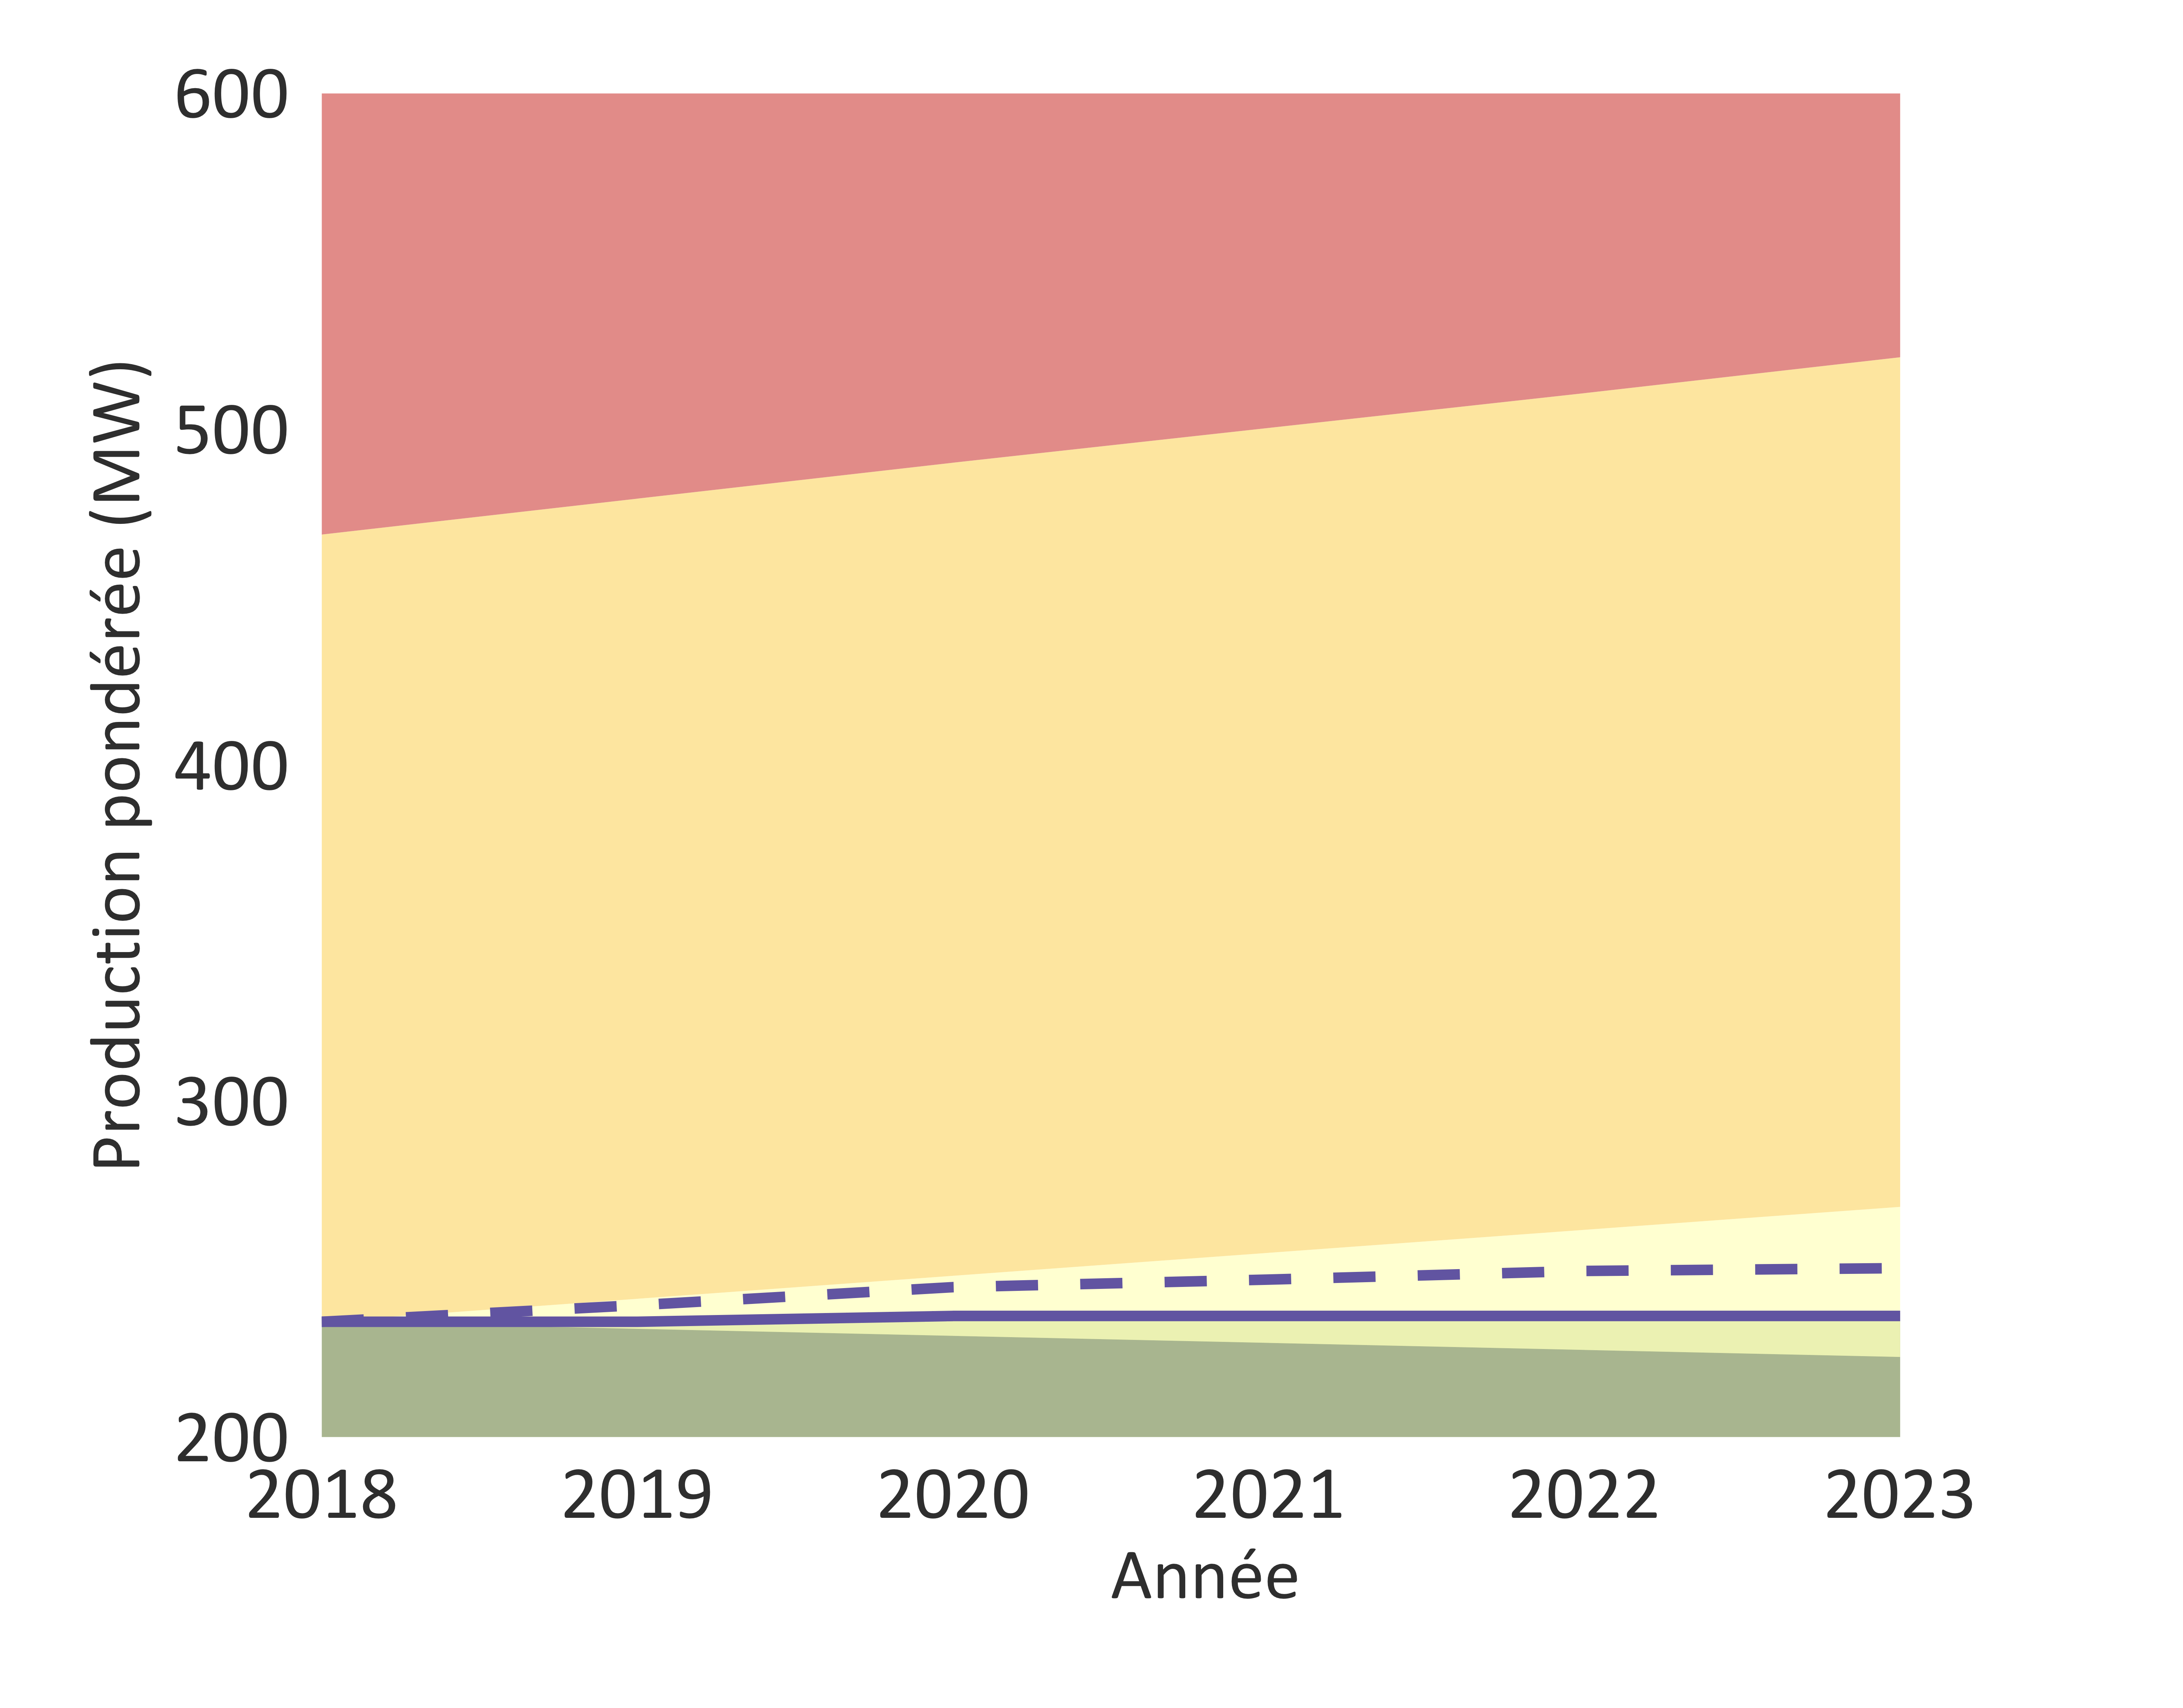
\includegraphics[trim = {0 0cm 0 0},width=1\linewidth]{ReportOutputs/Fig07}
		\vspace{-0.4cm}
		\begin{center}
		\textbf{Trajectoire de la capacité électrique issue des technologies renouvelables*}
		\end{center}
		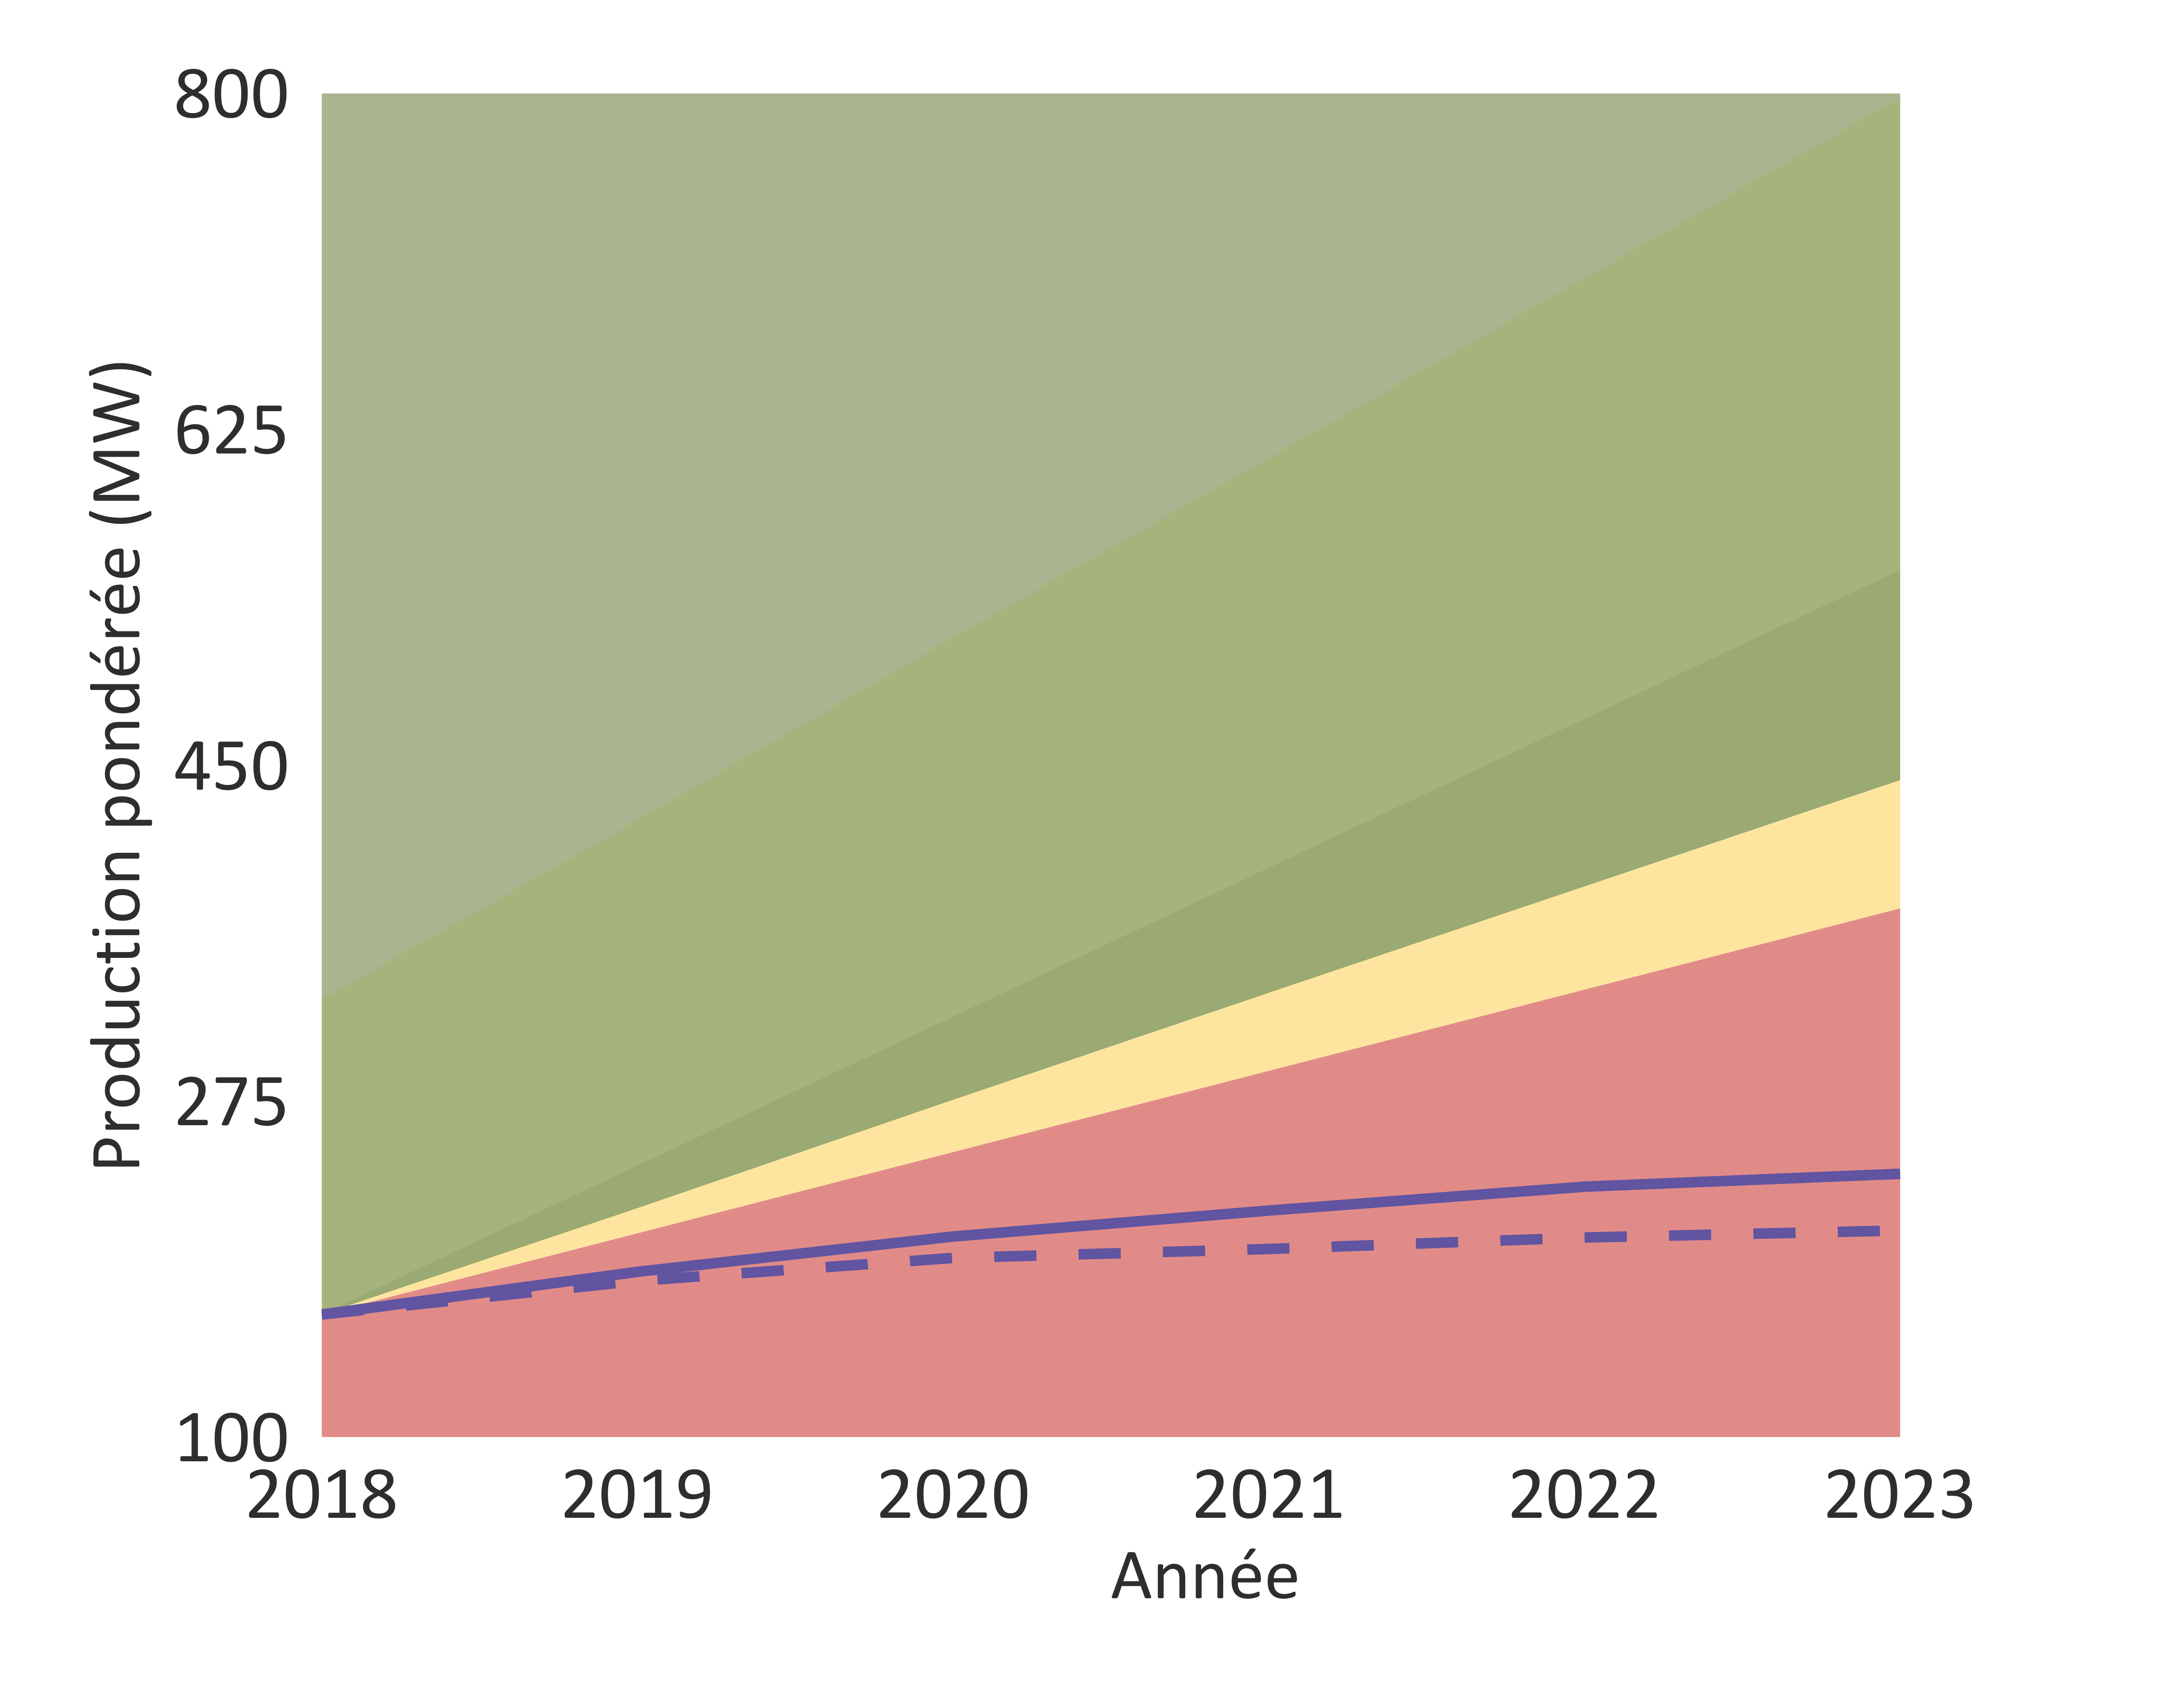
\includegraphics[trim = {0 0cm 0 0},width=.99\linewidth]{ReportOutputs/Fig08}
	\end{minipage}	
	\hspace{.02\linewidth}
	\begin{minipage}[t]{.49\textwidth}
		\begin{center}
		\textbf{Trajectoire de la capacité éléctrique issue du gaz}
		\end{center}
		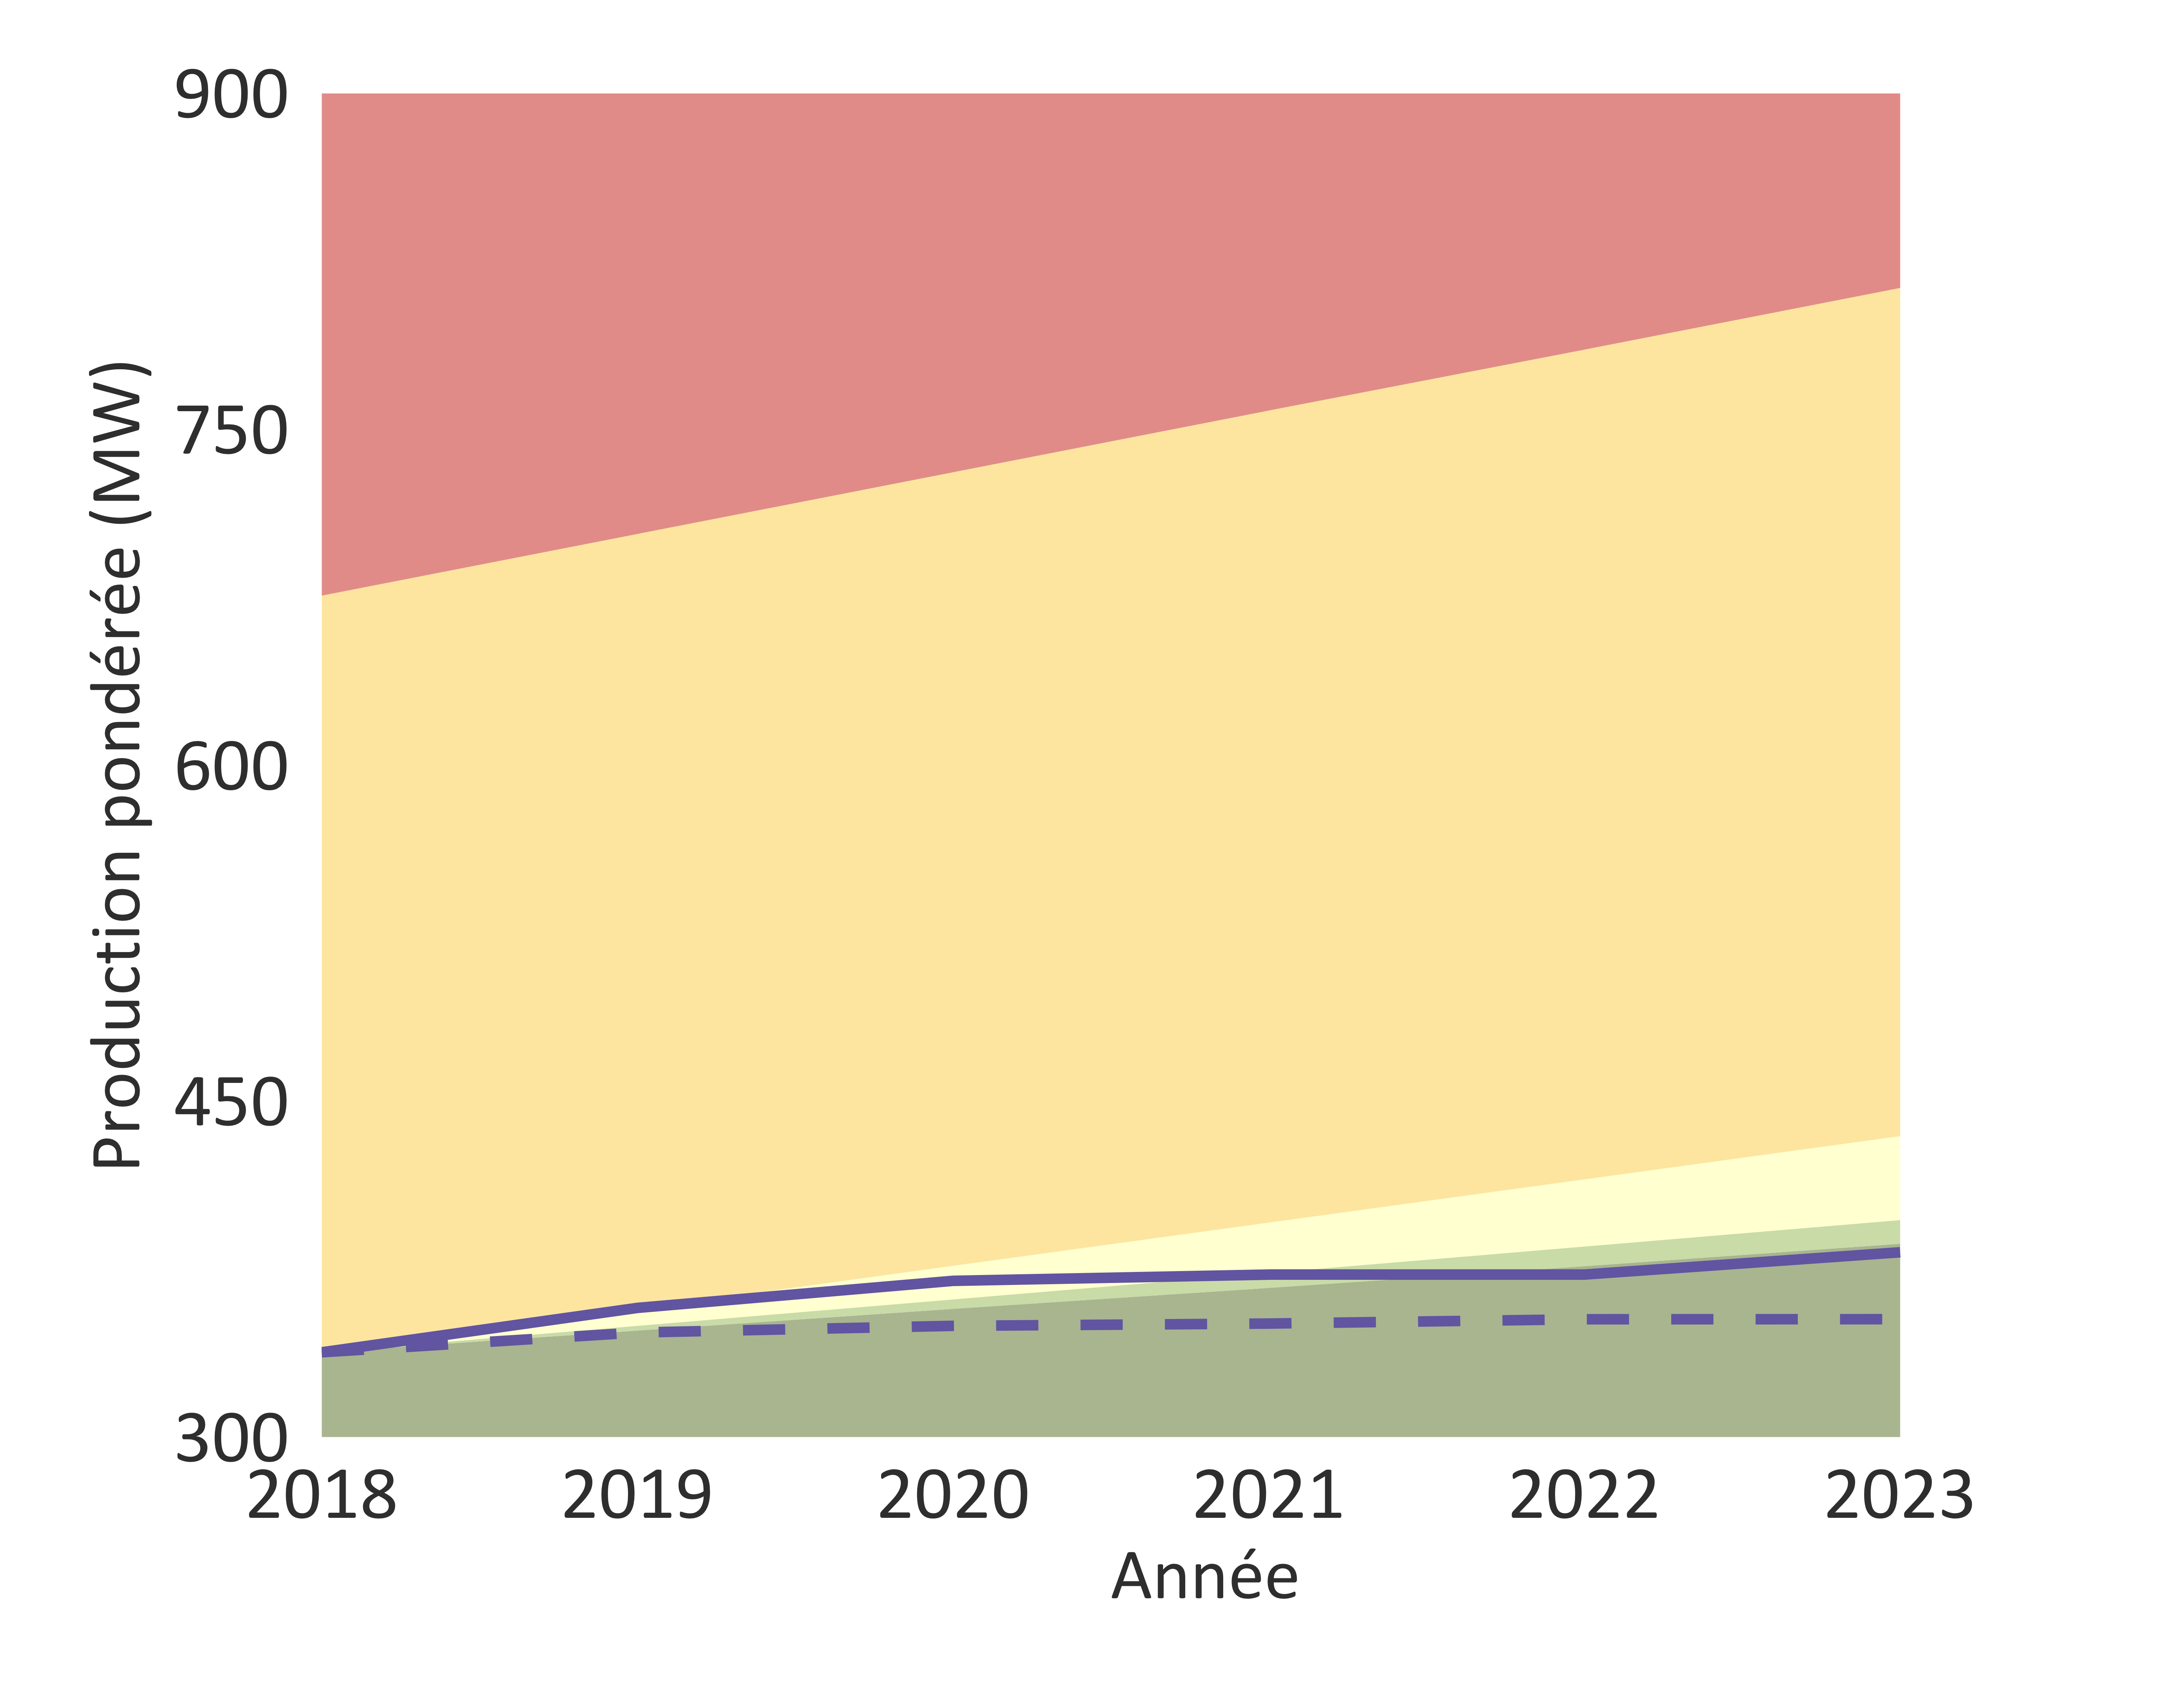
\includegraphics[trim = {0 0cm 0 0},width=1\linewidth]{ReportOutputs/Fig09}
		
		
		\vspace{0.1cm}
		\begin{center}
		\textbf{Trajectoire de la capacité électrique issue du nucléaire}
		\newline
		\end{center}
		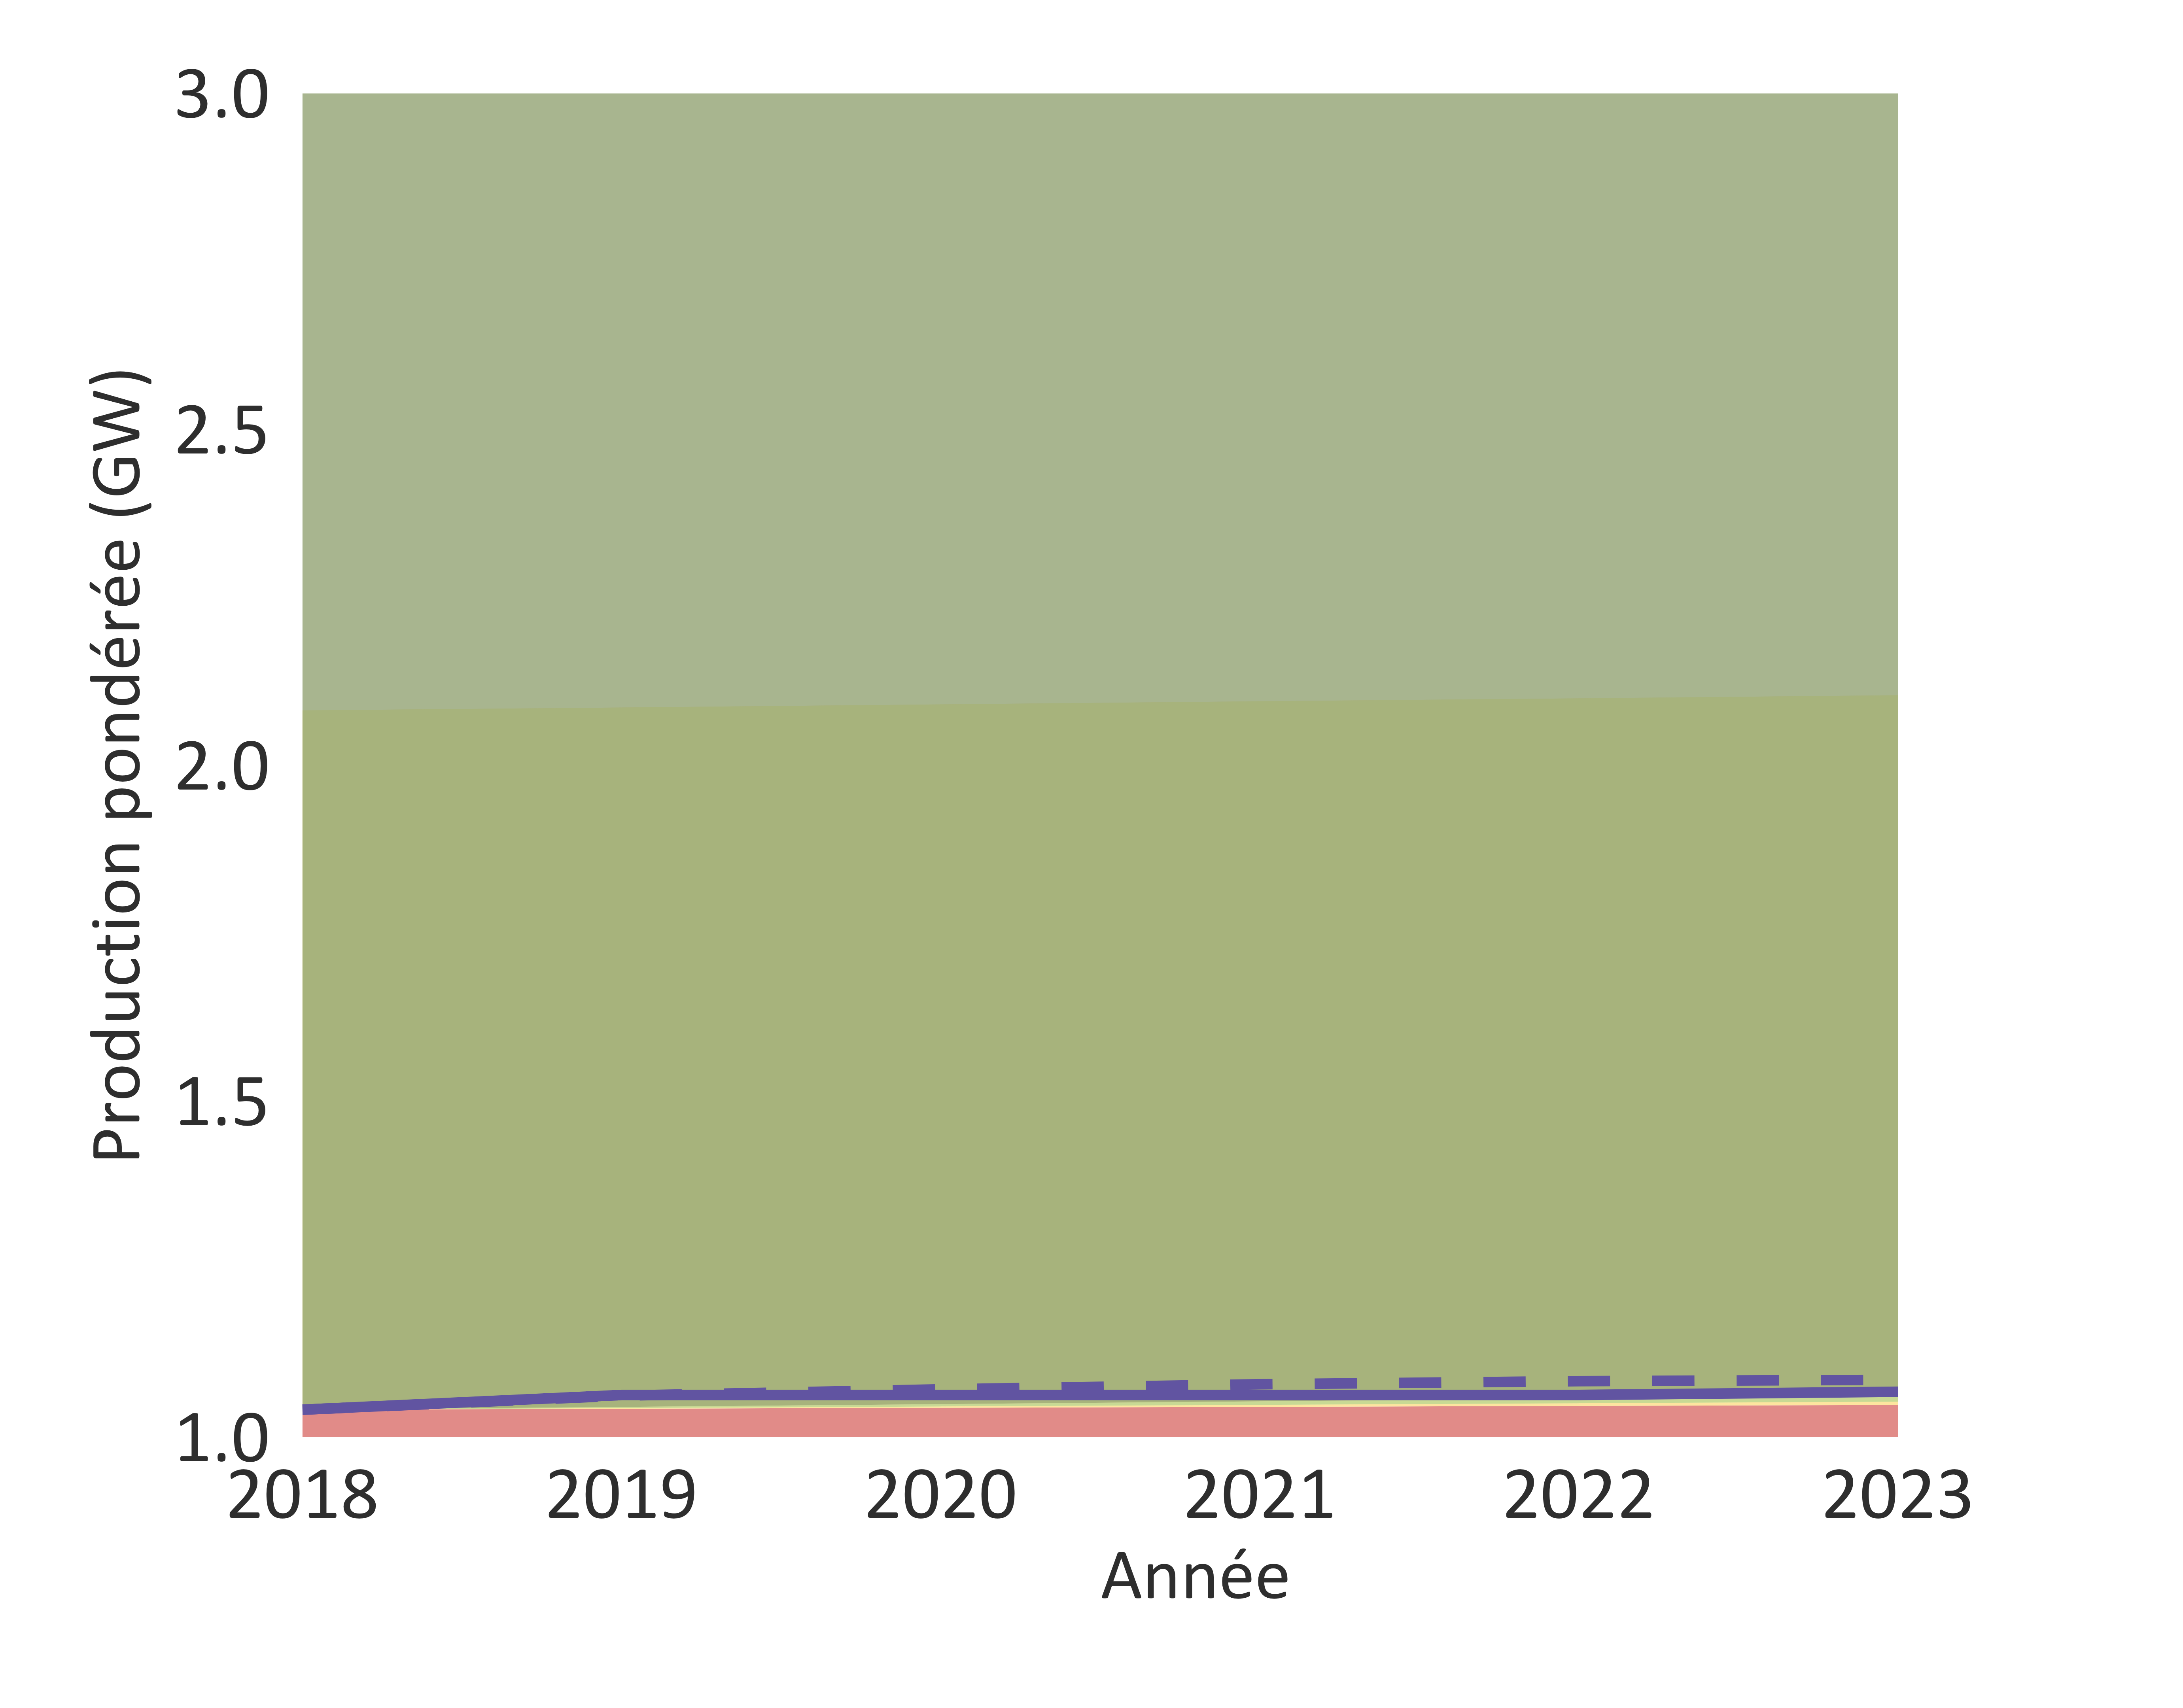
\includegraphics[trim = {0 0cm 0 0},width=1\linewidth]{ReportOutputs/Fig10}
		
		
	\end{minipage}
	
	\vspace{-0.6cm}
	\begin{center}
		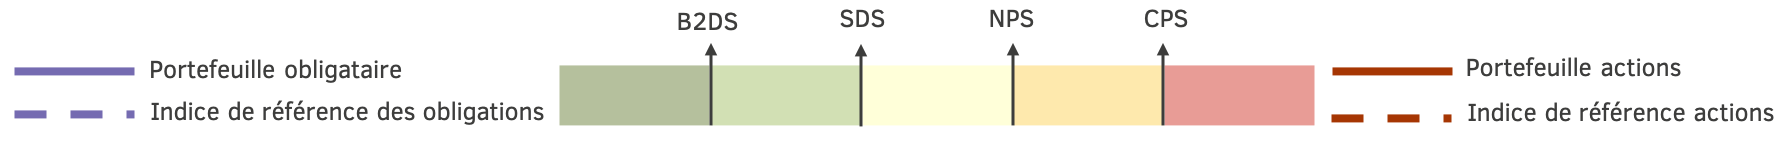
\includegraphics[trim = {0 0cm 0 0},width=1\linewidth]{ReportGraphics/246Legend_FR.png}
	\end{center}
	\vspace{-0.4cm}
	{\footnotesize\textit{*En raison des différences de suppositions concernant la combinaison de technologies dans le secteur de l'énergie renouvelable entre le B2DS et le SDS, le SDS peut sembler plus ambitieux pour les énergies renouvelables que le B2DS. toutefois, la production d'électricité à partir d'énergies renouvelables devrait toujours être supérieure dans le B2DS malgré la capacité inférieure.}}
		\vspace{-0.3cm}
	\PageFooterThird

	\newpage 
	%PowerSector_CBE
	%PowerSector_EQS
	\section*{} % TRAJECTORY - EQUITY - POWER  
	\HeaderDouble{TENDANCE A 5 ANS - ACTIONS}{ELECTRICITE}		
	\vspace{-0.3 cm}
	\begin{multicols}{2}
	\textbf{Les graphiques ci-dessous illustrent l'alignement du portefeuille actions pour les technologies de production d’électricité sélectionnés par rapport aux scénarios de transition de l'AIE: B2DS, SDS, NPS, CPS et l´indice de référence actions.}\\
	Pour chaque technologie, la valeur tracée pour le portefeuille (ligne continue) est l'évolution estimée ou la « trajectoire » de la capacité installée allouée au portefeuille actions sur les 5 prochaines années.
	Les lignes séparant les zones d'arrière-plan délimitées par couleur représentent la « production cible » du portefeuille pour chaque technologie selon les scénarios de l'AIE. La ligne en pointillés montre la trajectoire prévue de la capacité installée du indice de référence actions pour chaque technologie, mise à l'échelle du portefeuille, pour faciliter la comparaison.
		                    
		
	\end{multicols}
\vspace{-0.3cm}
	\begin{minipage}[t]{.49\linewidth}
			\begin{center}
		\textbf{Trajectoire de la capacité électrique issue du charbon }
			\end{center}
		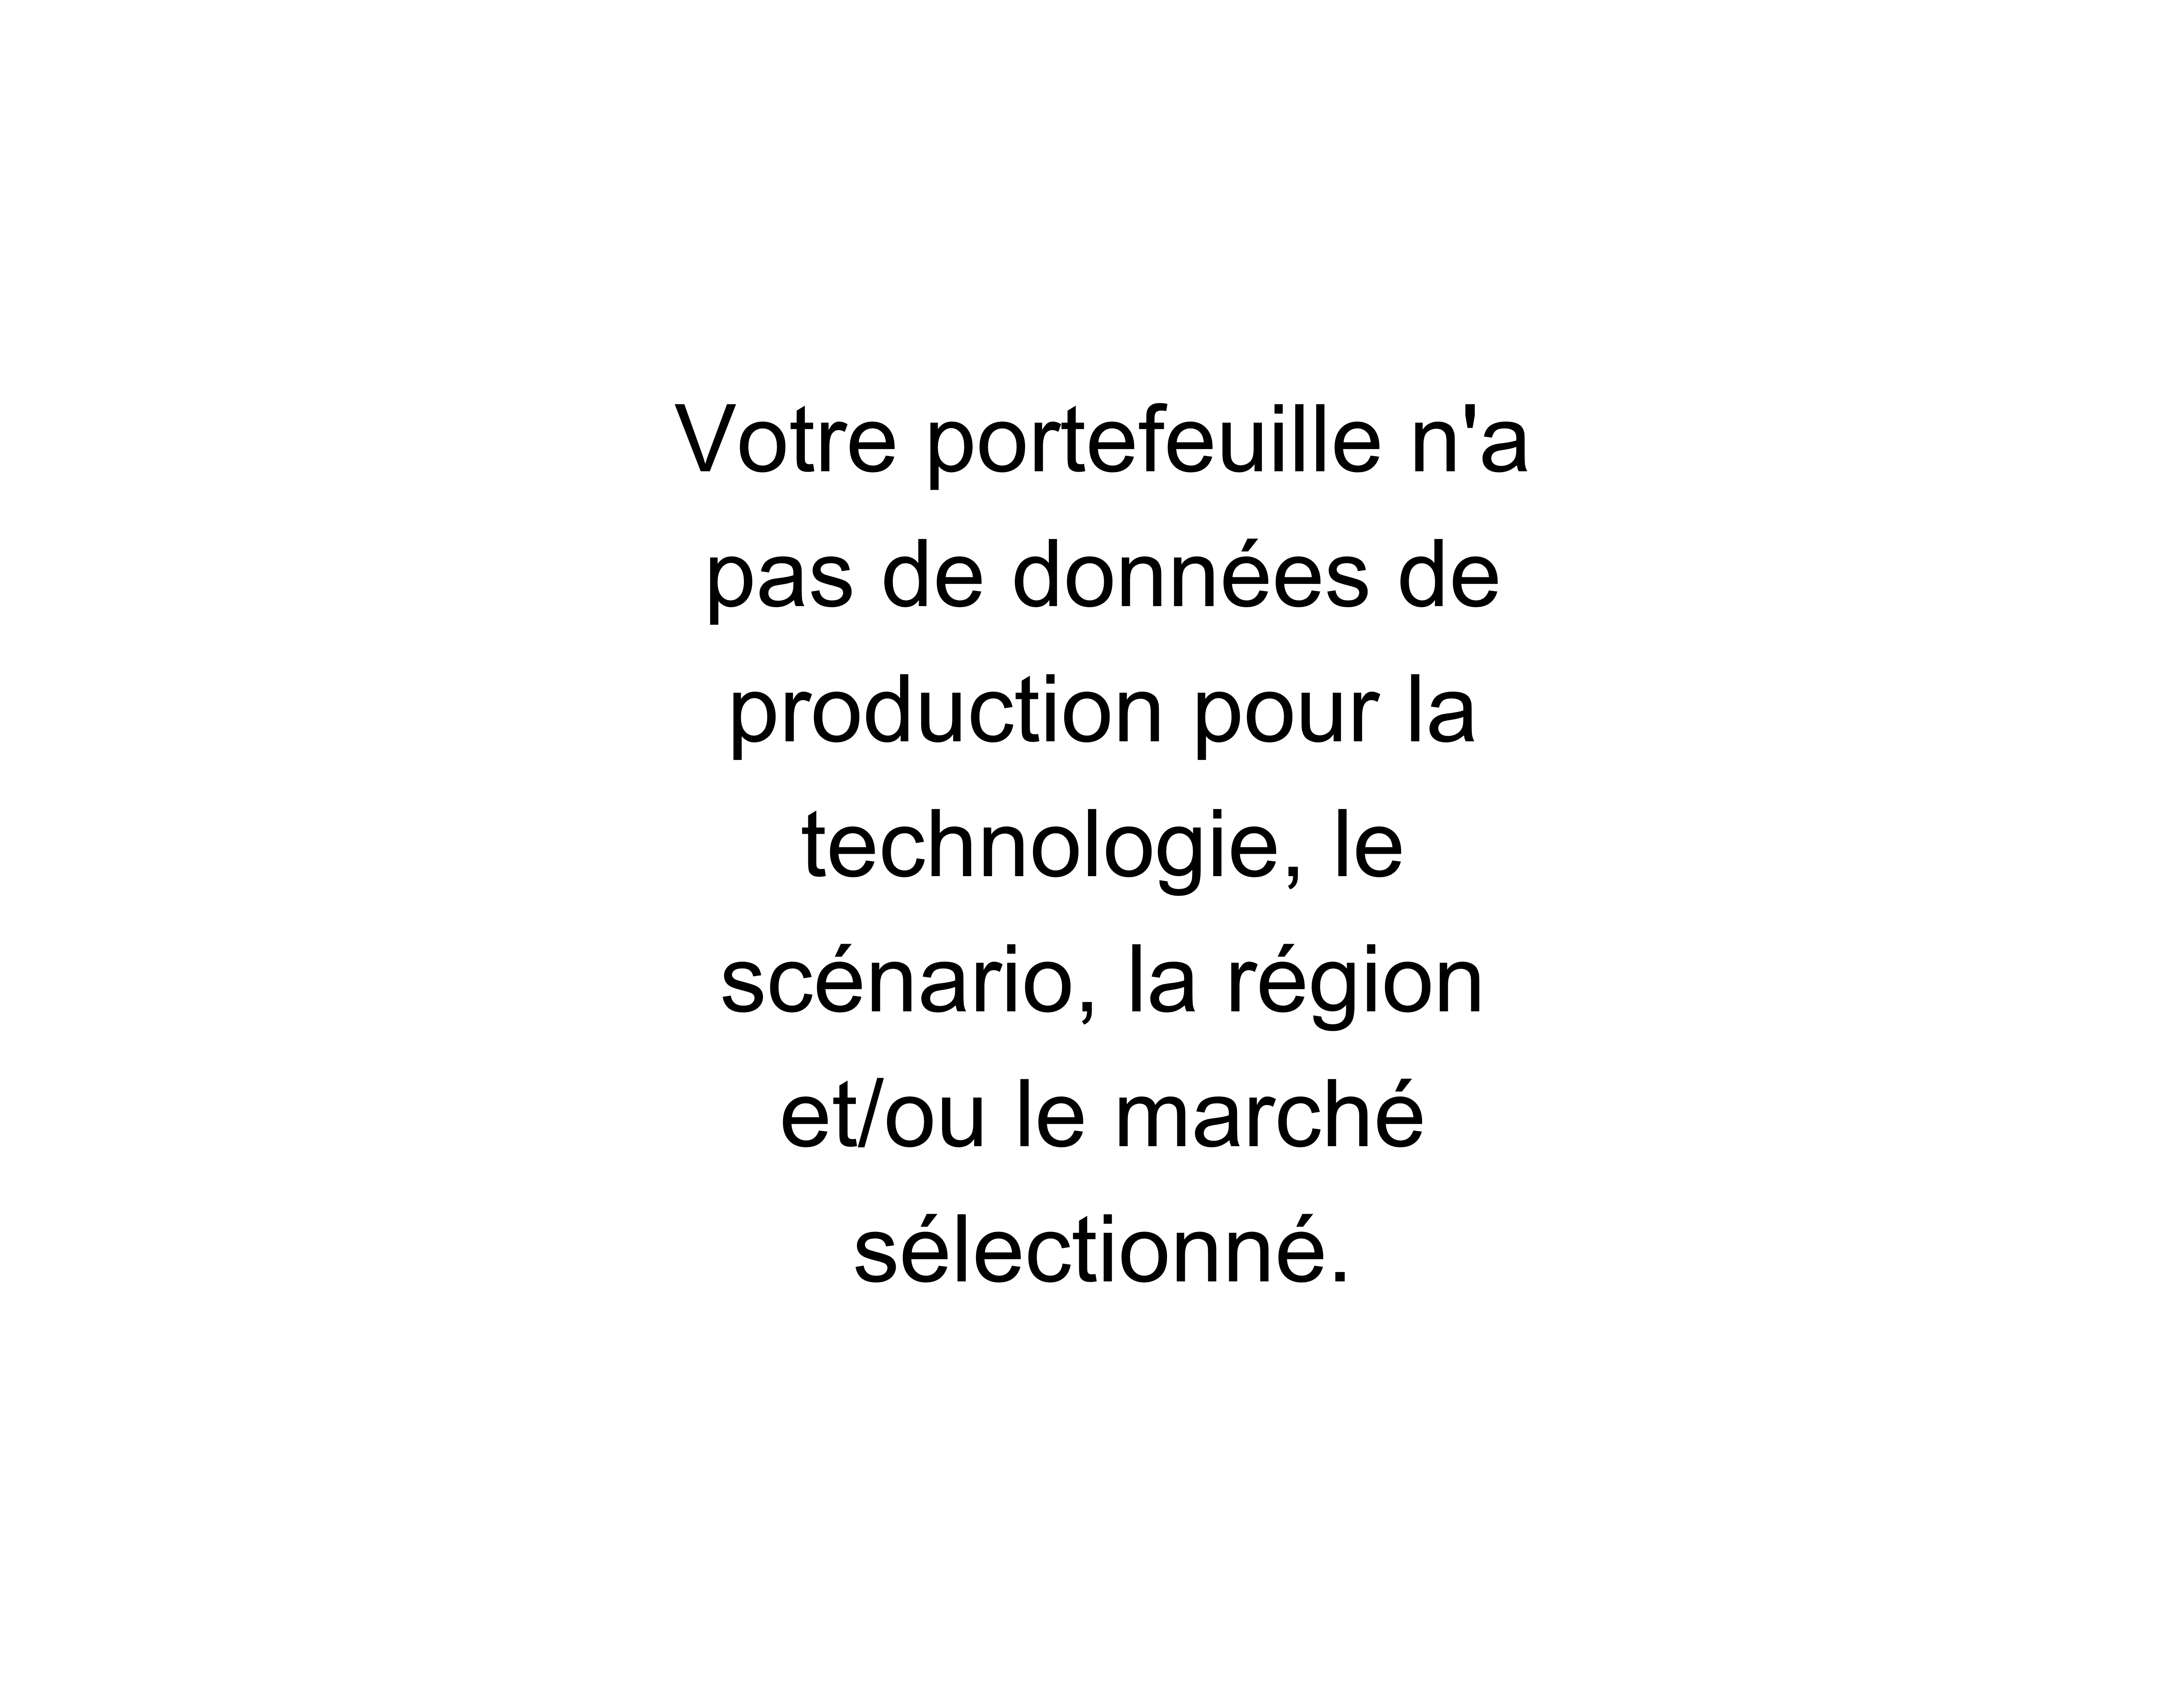
\includegraphics[trim = {0 0cm 0 0},width=1\linewidth]{ReportOutputs/Fig17}
		\vspace{-0.4cm}
			\begin{center}
		\textbf{Trajectoire de la capacité électrique issue des technologies renouvelables* }
			\end{center}
		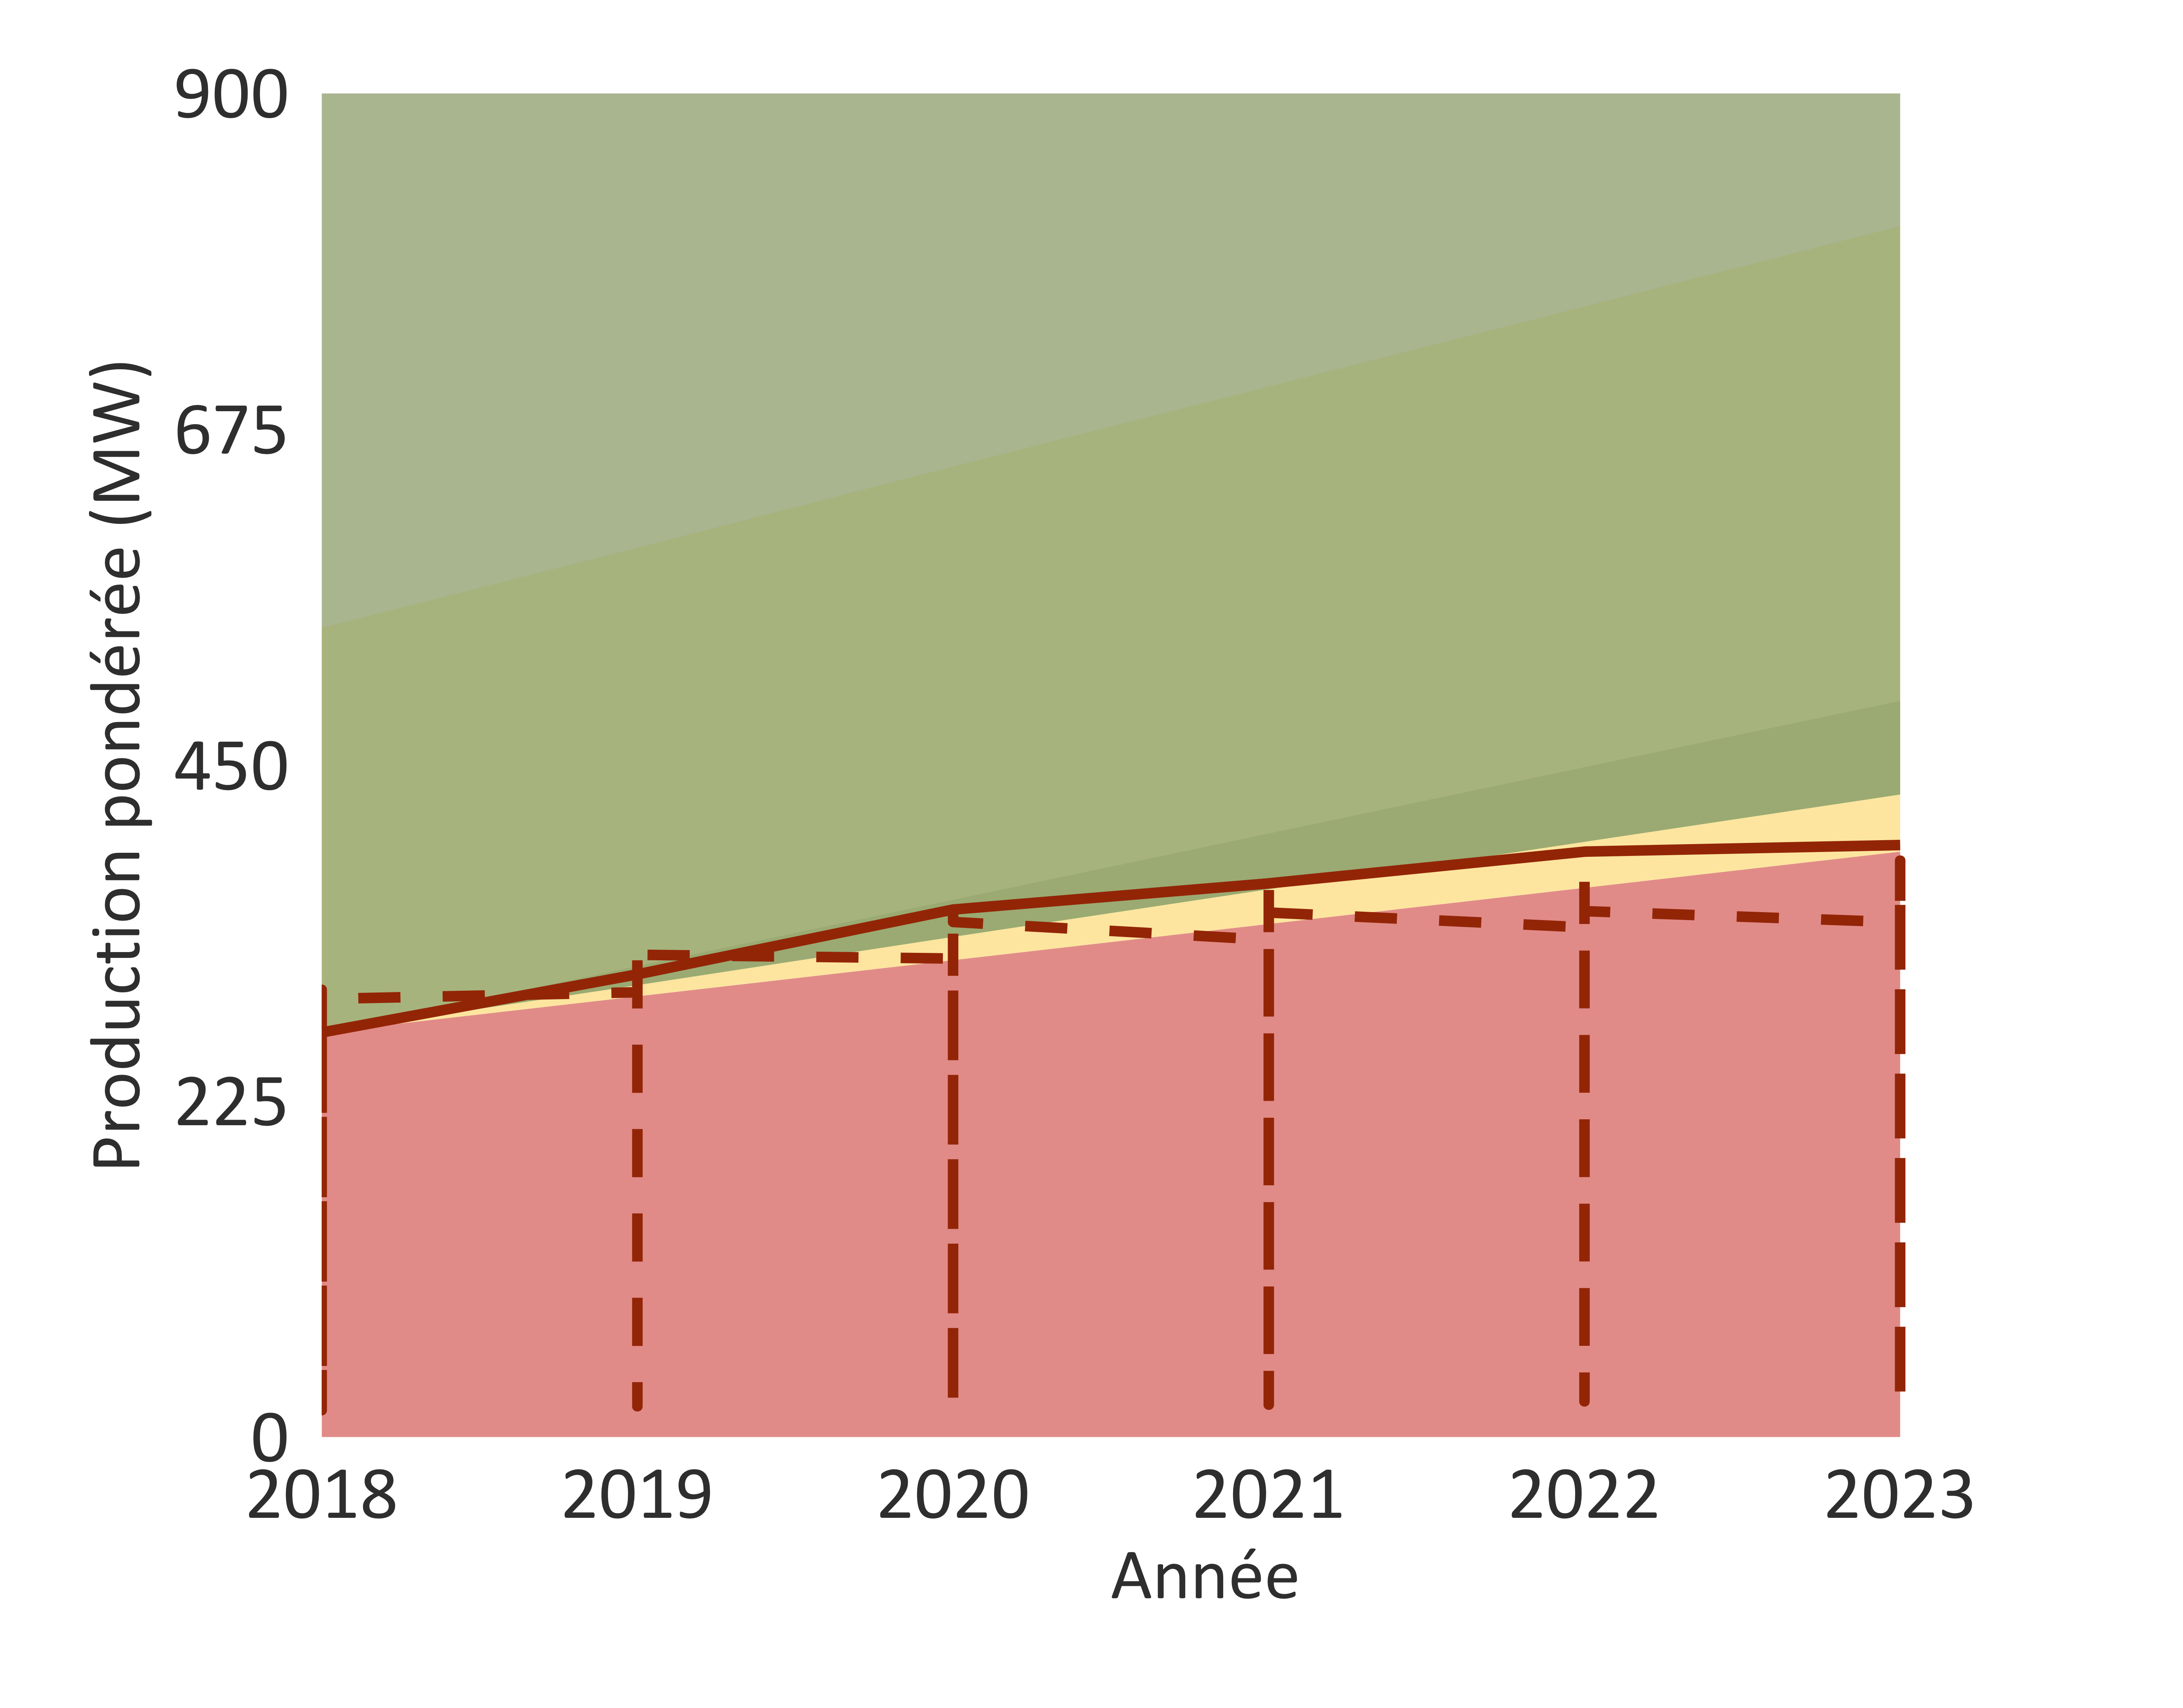
\includegraphics[trim = {0 0cm 0 0},width=.99\linewidth]{ReportOutputs/Fig18}
	\end{minipage}	
	\hspace{.02\linewidth}
	\begin{minipage}[t]{.49\textwidth}
			\begin{center}
		\textbf{Trajectoire de la capacité éléctrique issue du gaz}
			\end{center}
		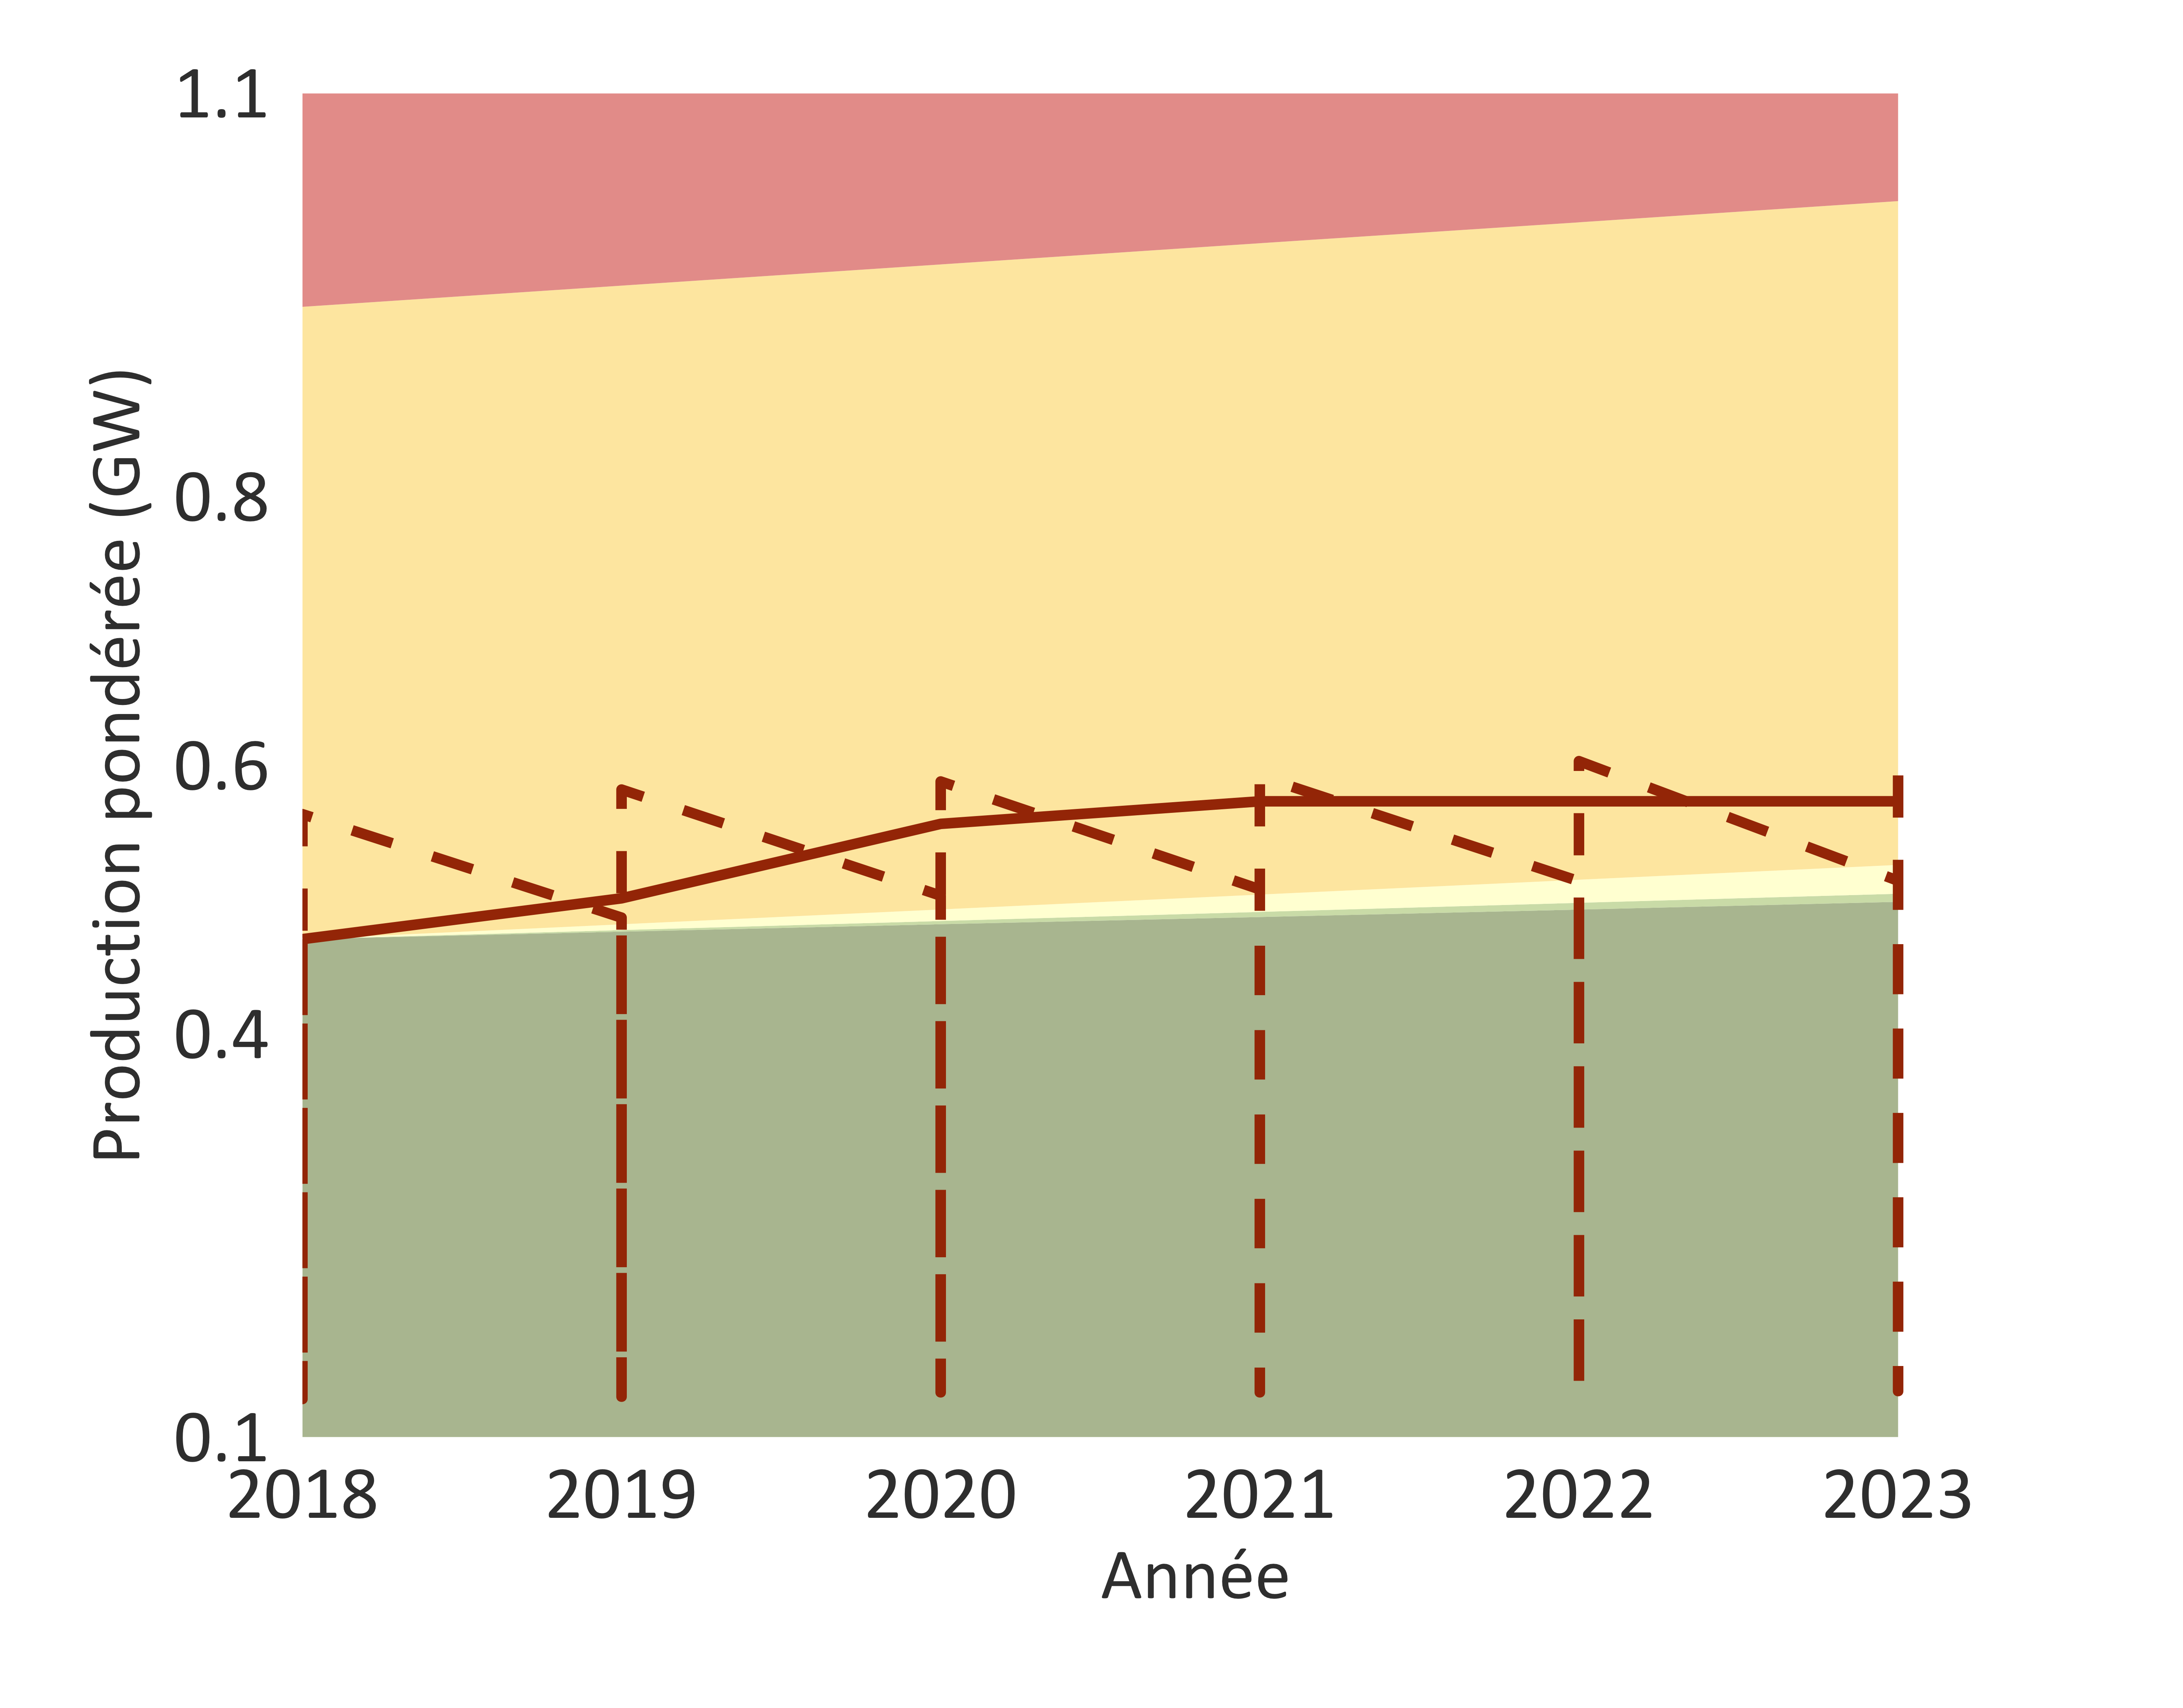
\includegraphics[trim = {0 0cm 0 0},width=1\linewidth]{ReportOutputs/Fig19}
		
		
		\vspace{0.1cm}
			\begin{center}
		\textbf{Trajectoire de la capacité électrique issue du nucléaire} 
		\newline
			\end{center}
		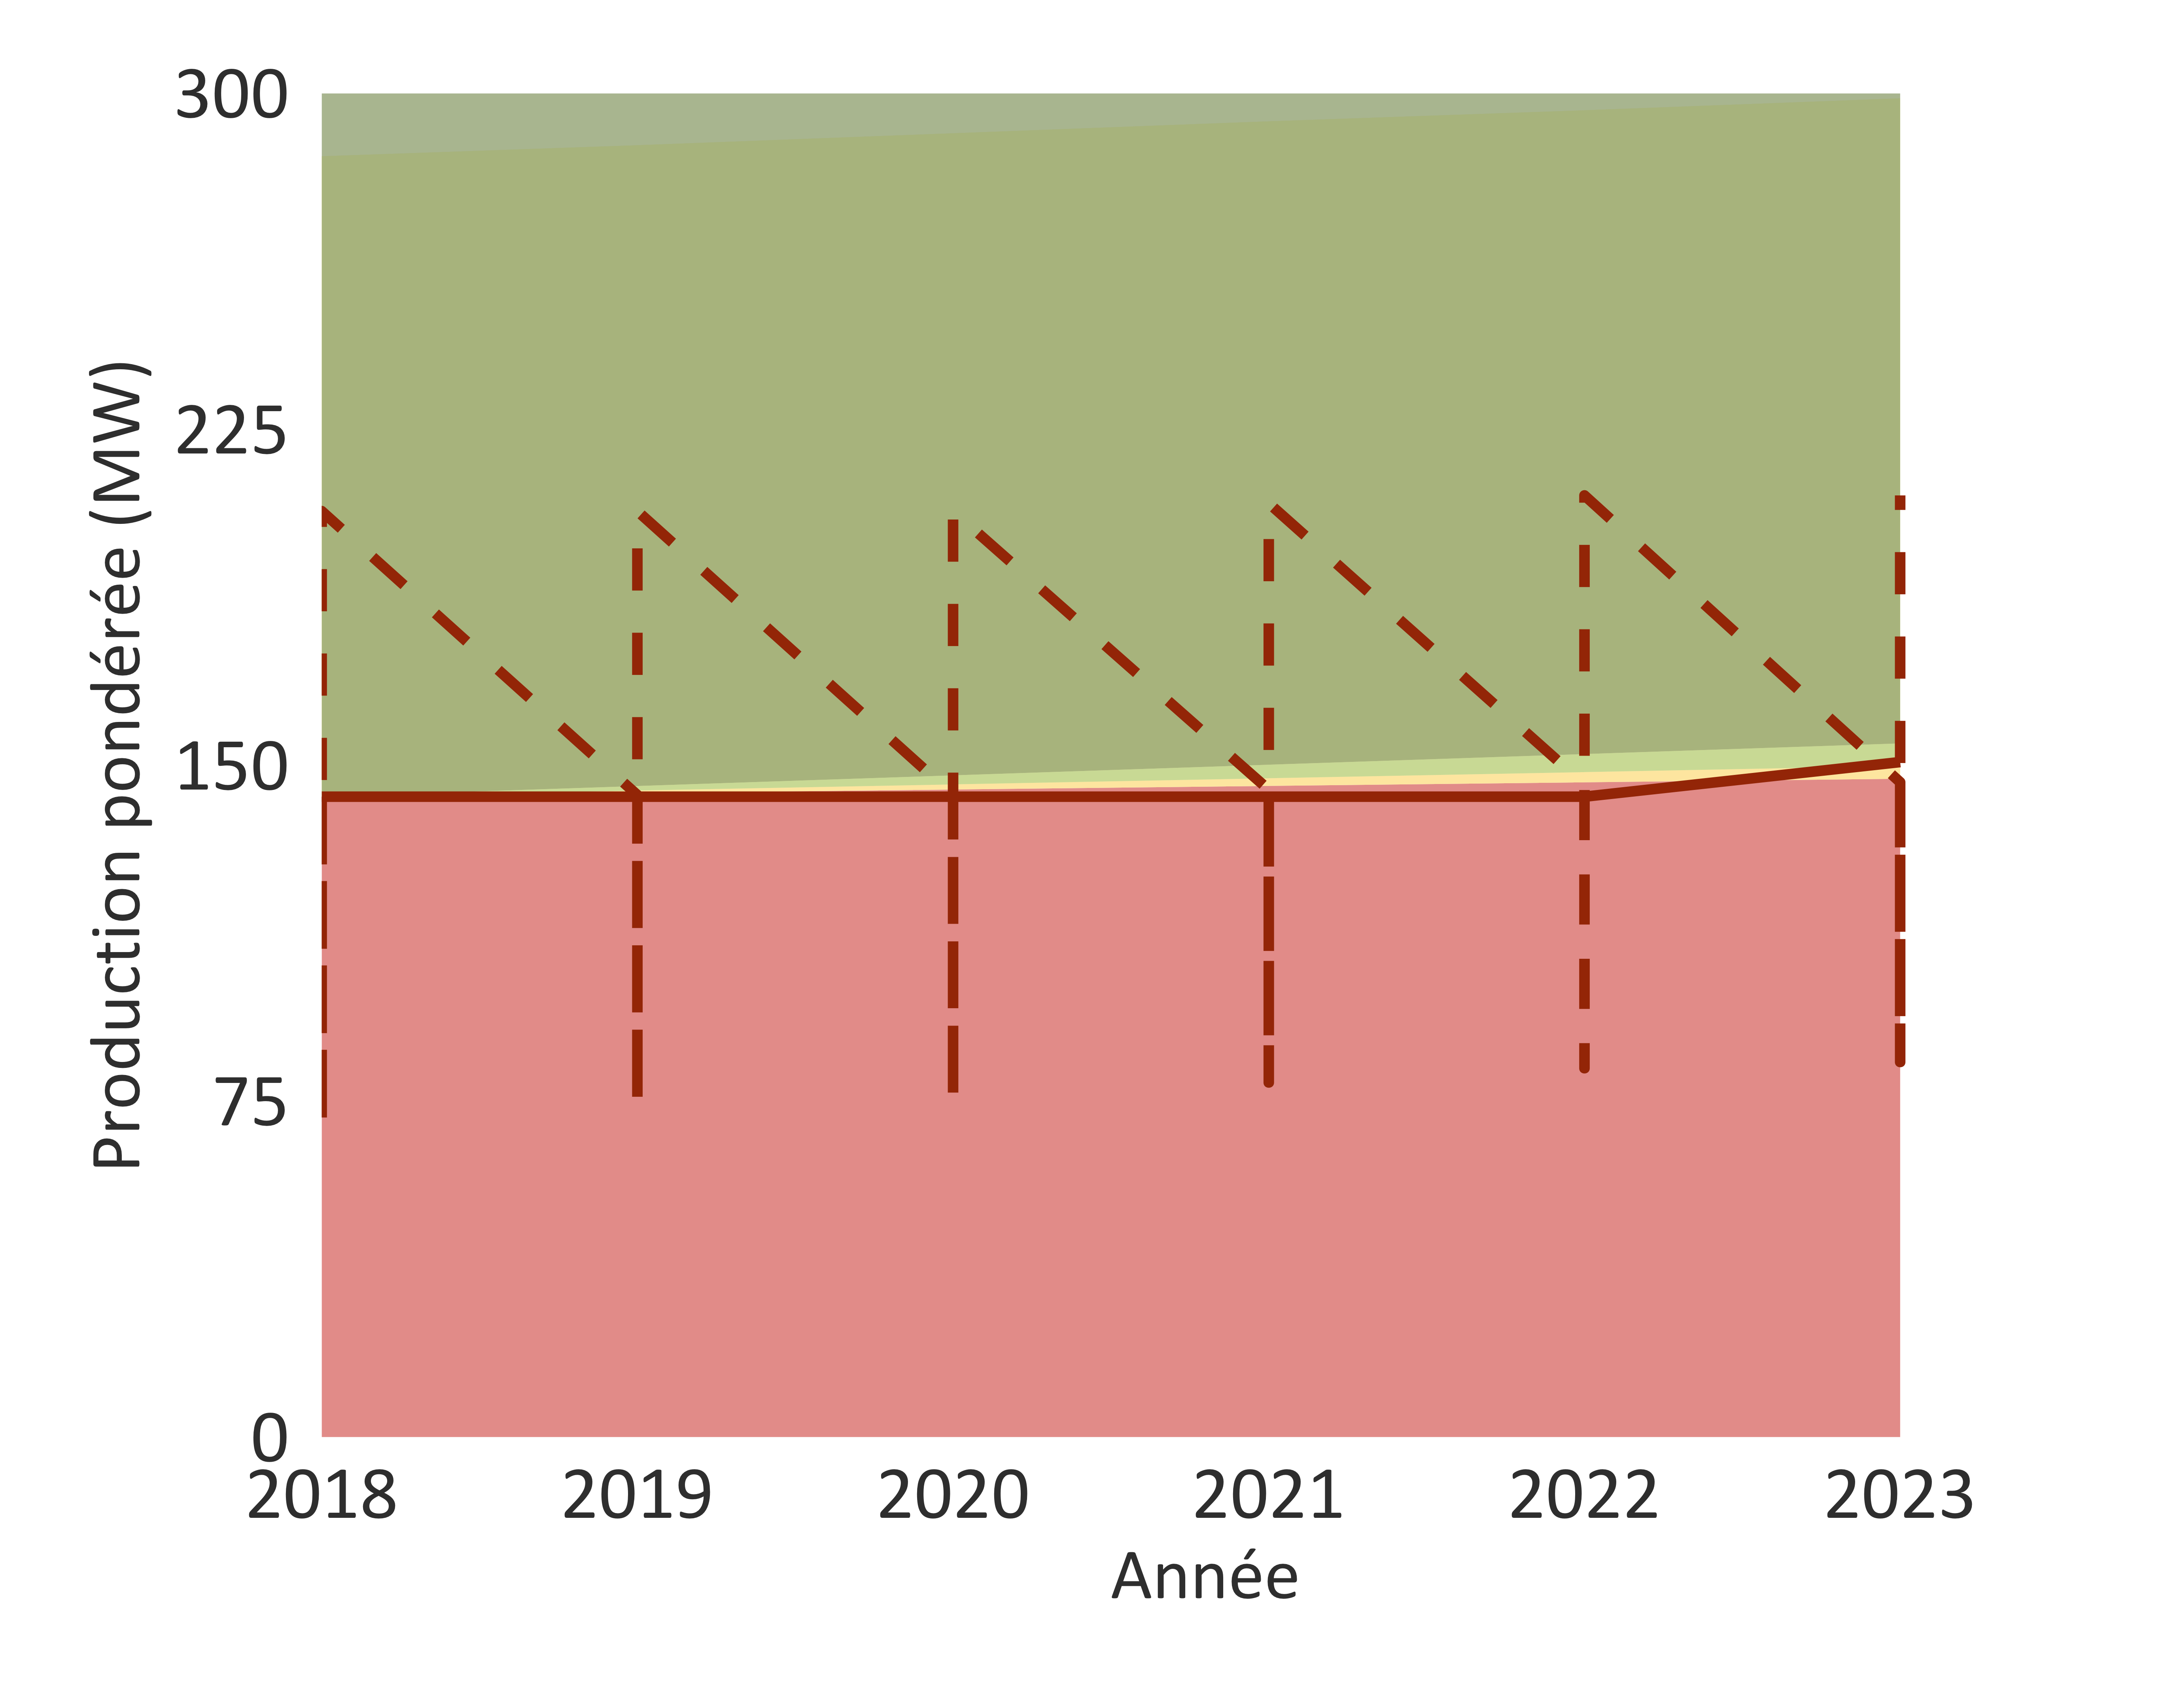
\includegraphics[trim = {0 0cm 0 0},width=1\linewidth]{ReportOutputs/Fig20}
		
		
	\end{minipage}
	
	\vspace{-0.6cm}
	\begin{center}
		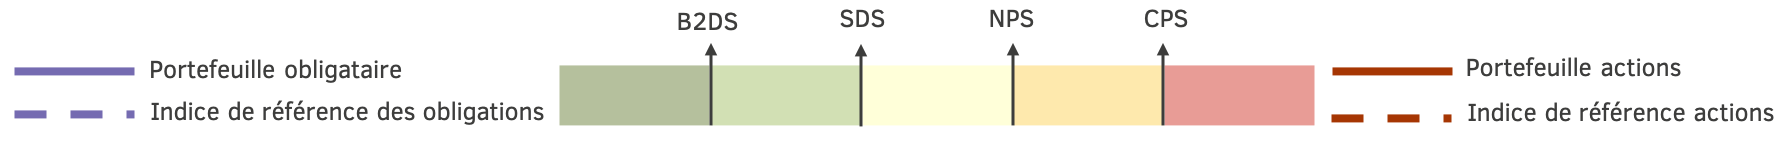
\includegraphics[trim = {0 0cm 0 0},width=1\linewidth]{ReportGraphics/246Legend_FR.png}
	\end{center}
 \vspace{-0.4cm}
	{\footnotesize\textit{*En raison des différences de suppositions concernant la combinaison de technologies dans le secteur de l'énergie renouvelable entre le B2DS et la SDS, la SDD peut sembler plus ambitieuse pour les énergies renouvelables que la B2DS. toutefois, la production d'électricité à partir d'énergies renouvelables devrait toujours être supérieure dans le B2DS malgré la capacité réduite.}}
	 \vspace{-0.3cm}
	
	\PageFooterThird
	\newpage 
	%PowerSector_EQE
	%PowerSector_ALLE

	%FossilFuelSector_ALLS
	%FossilFuelSector_CBS
	\section*{} % TRAJECTORY - DEBT - FOSSIL FUELS AND AUTOMOTIVE   
	\HeaderDouble{TENDANCE A 5 ANS- OBLIGATIONS}{ENERGIES FOSSILES}	
	
	\begin{multicols}{2}
		\textbf{Les graphiques ci-dessous illustrent l'alignement du combustibles fossiles du portefeuille obligataire par rapport aux scénarios de transition de l'AIE: B2DS, SDS, NPS, CPS. et le marché obligataire.}\\
		Pour chaque technologie, la valeur tracée pour le portefeuille (ligne continue) est l'évolution estimée ou la « trajectoire » de la production allouée au portefeuille d'obligations d’entreprises sur les 5 prochaines années. 
		Les lignes séparant les zones d'arrière-plan délimitées par couleur représentent la « production cible » du portefeuille pour chaque technologie selon les scénarios de l'AIE. La ligne en pointillés montre la trajectoire prévue de la capacité installée pour le marché obligataire pour chaque technologie, mise à l'échelle du portefeuille, pour faciliter la comparaison.
			                 
		
		
	\end{multicols}		
	
	%\begin{center}
	%	\textbf{Secteur De Energie fossile}
	%\end{center}
	
	\begin{minipage}[t]{.49\linewidth}
		\begin{center}
		\textbf{Trajectoire de la production de pétrole }
	   \end{center}
		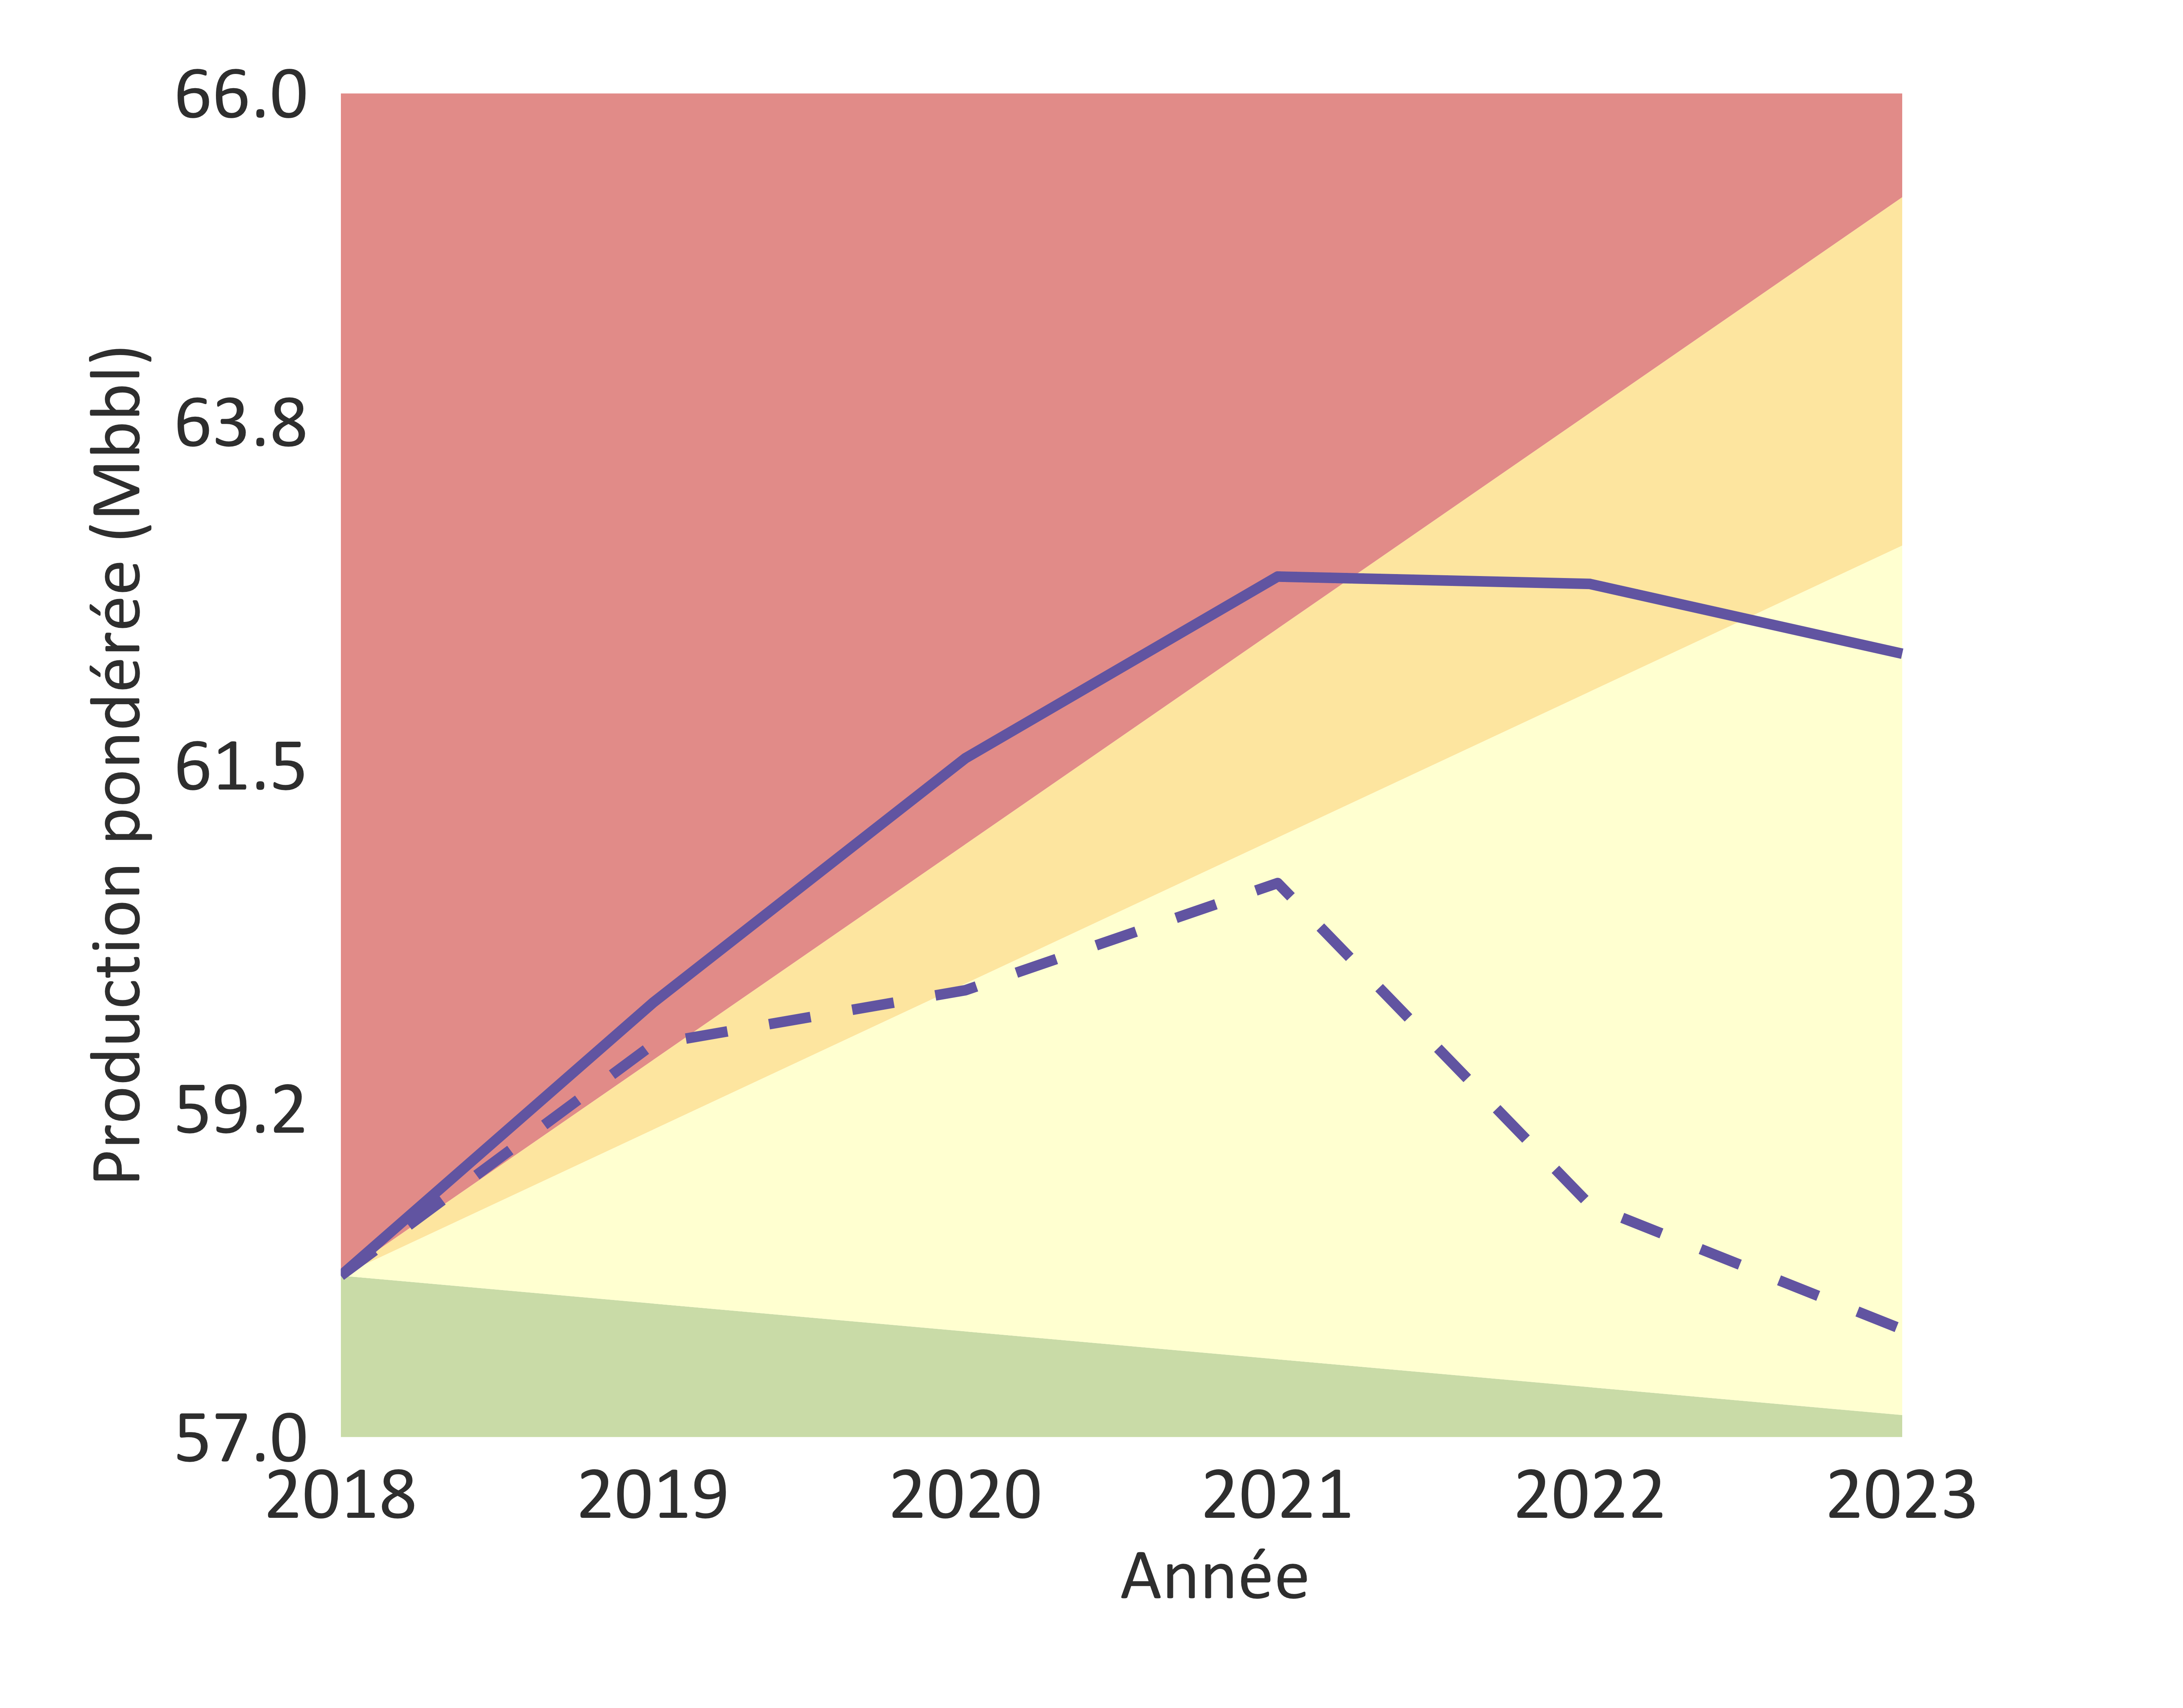
\includegraphics[trim = {0 0cm 0 0},width=1\linewidth]{ReportOutputs/Fig11}
		
	\end{minipage}	
	\hspace{.02\linewidth}
	\begin{minipage}[t]{.49\textwidth}
		\begin{center}
		\textbf{Trajectoire de la production de gaz }
	   \end{center}
		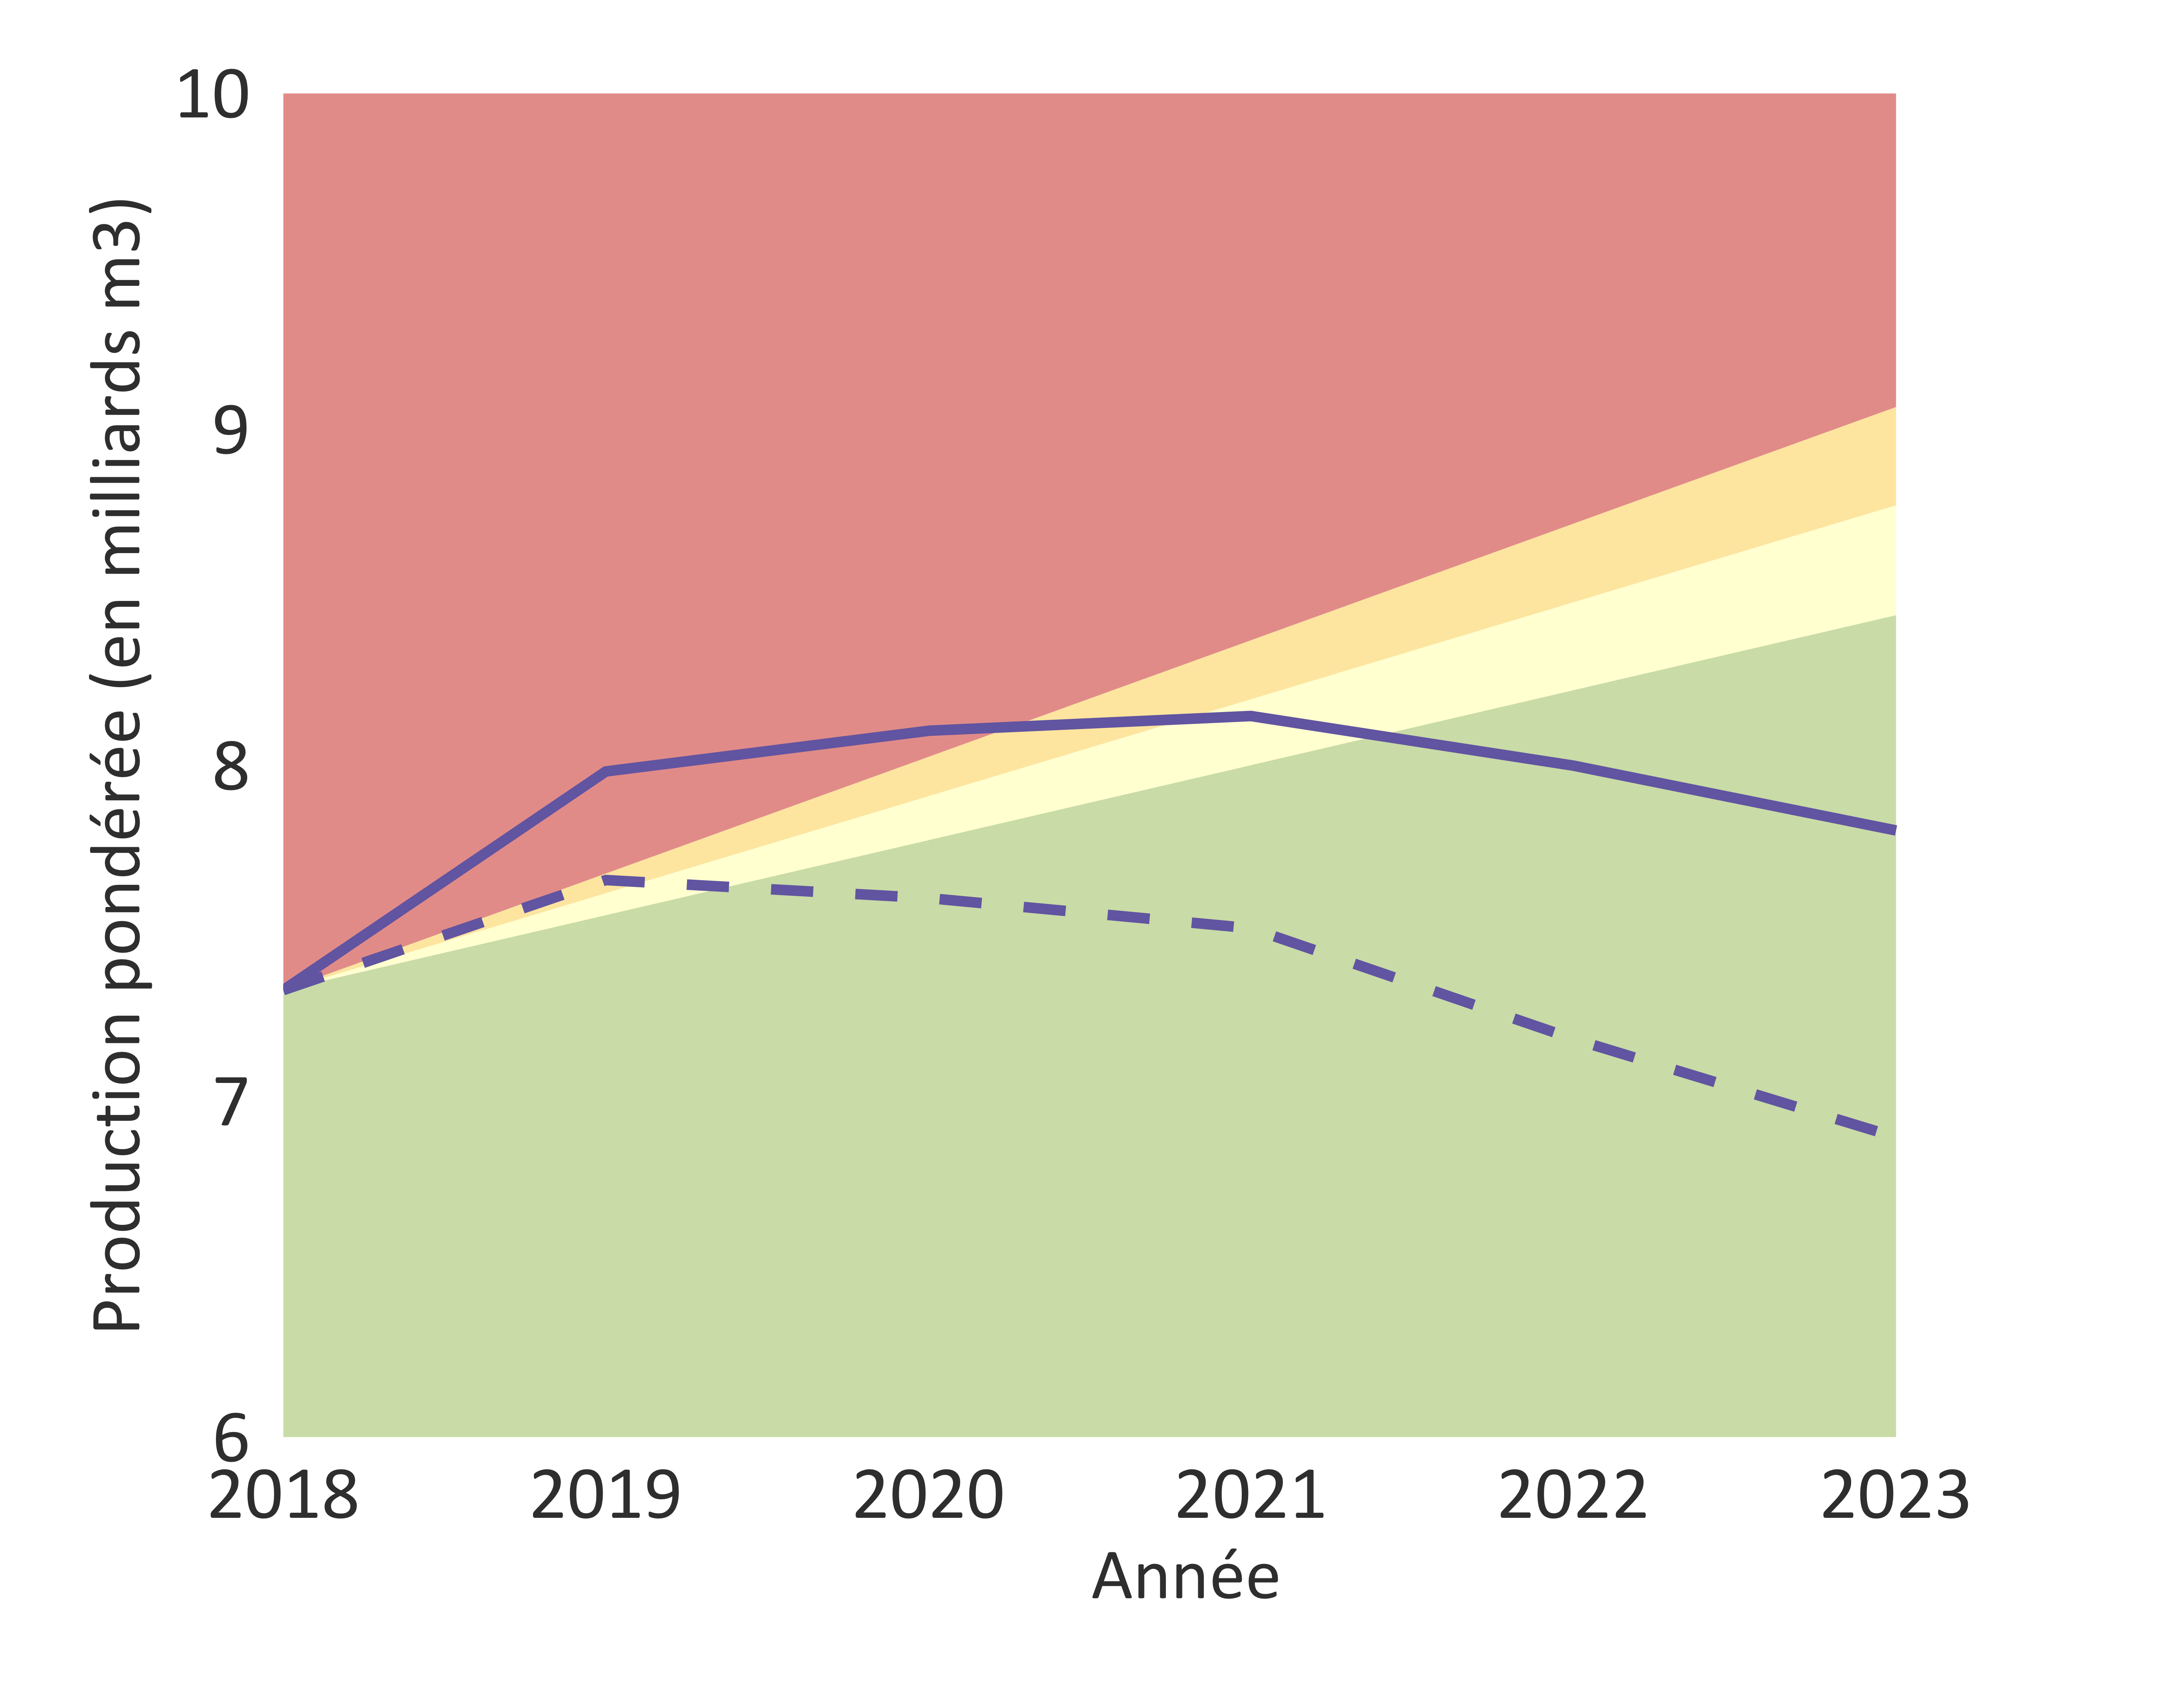
\includegraphics[trim = {0 0cm 0 0},width=1\linewidth]{ReportOutputs/Fig12}
		
	\end{minipage}
	
	

	\begin{minipage}[t]{.49\linewidth}
		\begin{center}
		\textbf{Trajectoire de la production de charbon}
	    \end{center}
		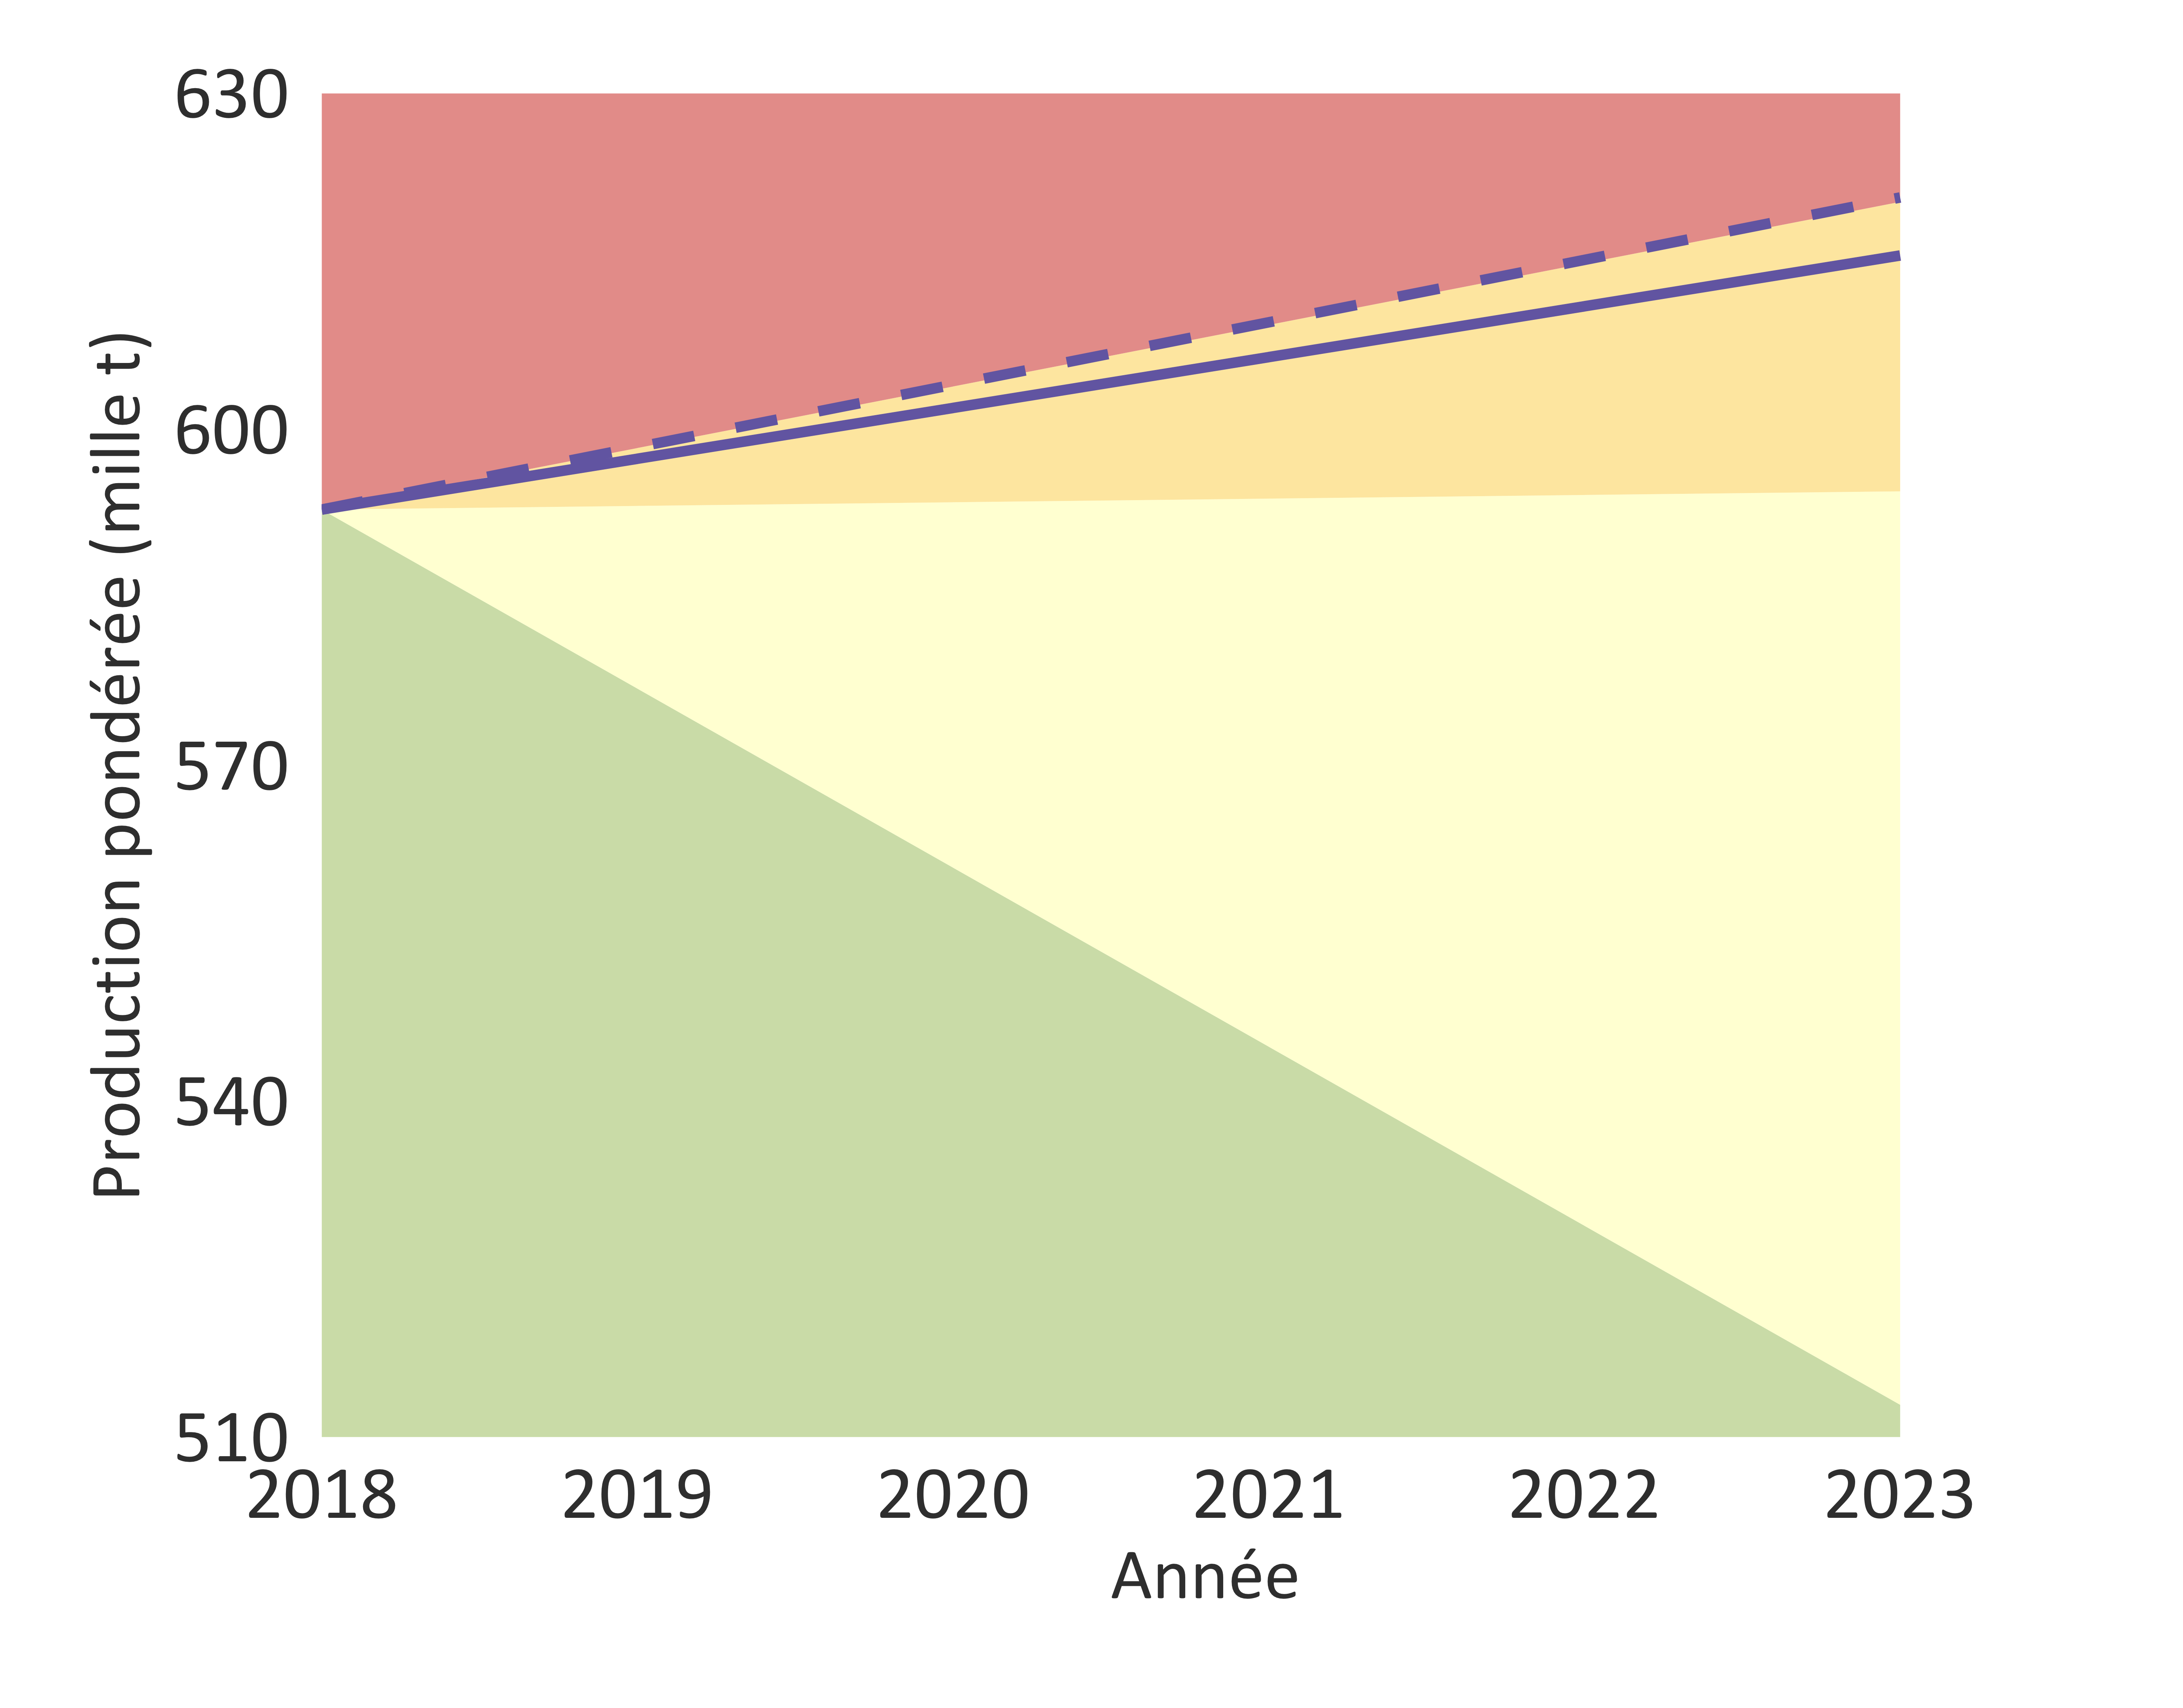
\includegraphics[trim = {0 0cm 0 0},width=1\linewidth]{ReportOutputs/Fig13}
		
	\end{minipage}	
		
	
	\vspace{-.1cm}
	\begin{center}
		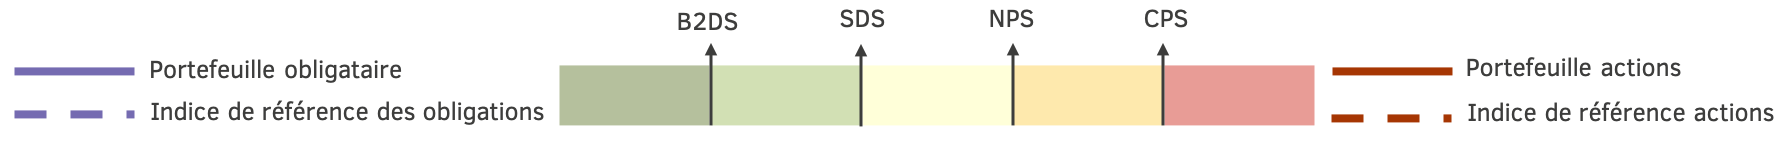
\includegraphics[trim = {0 0cm 0 0},width=1\linewidth]{ReportGraphics/246Legend_FR.png}
	\end{center}

	
	\PageFooterThird
	\newpage 

	%FossilFuelSector_CBE
	%FossilFuelSector_EQS 
	\section*{} % TRAJECTORY - EQUITY - FOSSIL FUELS AND AUTOMOTIVE  
	\HeaderDouble{TENDANCE A 5 ANS - ACTIONS}{ENERGIES FOSSILES}	
	
	\begin{multicols}{2}
		\textbf{Les graphiques ci-dessous illustrent l'alignement du portefeuille actions pour les énergies fossiles par rapport aux scénarios de transition de l'AIE: B2DS, SDS, NPS, CPS et l´indice de référence actions.}\\ 
		Pour chaque technologie, la valeur tracée pour le portefeuille (ligne continue) correspond à l'évolution ou à la « trajectoire » prévue de la production de combustibles fossiles allouée au portefeuille actions au cours des 5 prochaines années. 
		Les lignes séparant les zones d'arrière-plan délimitées par couleur représentent la « production cible » du portefeuille pour chaque technologie selon les scénarios de l'AIE. La ligne en pointillés montre la trajectoire prévue de la capacité installée pour le indice de référence actions pour chaque technologie, mise à l'échelle du portefeuille, pour faciliter la comparaison.
	\end{multicols}		

	%\begin{center}
	%	\textbf{Secteur De Energie fossile}
	%\end{center}
	
	\begin{minipage}[t]{.49\linewidth}
	\begin{center}
		\textbf{Trajectoire de la production de pétrole }
	\end{center}
		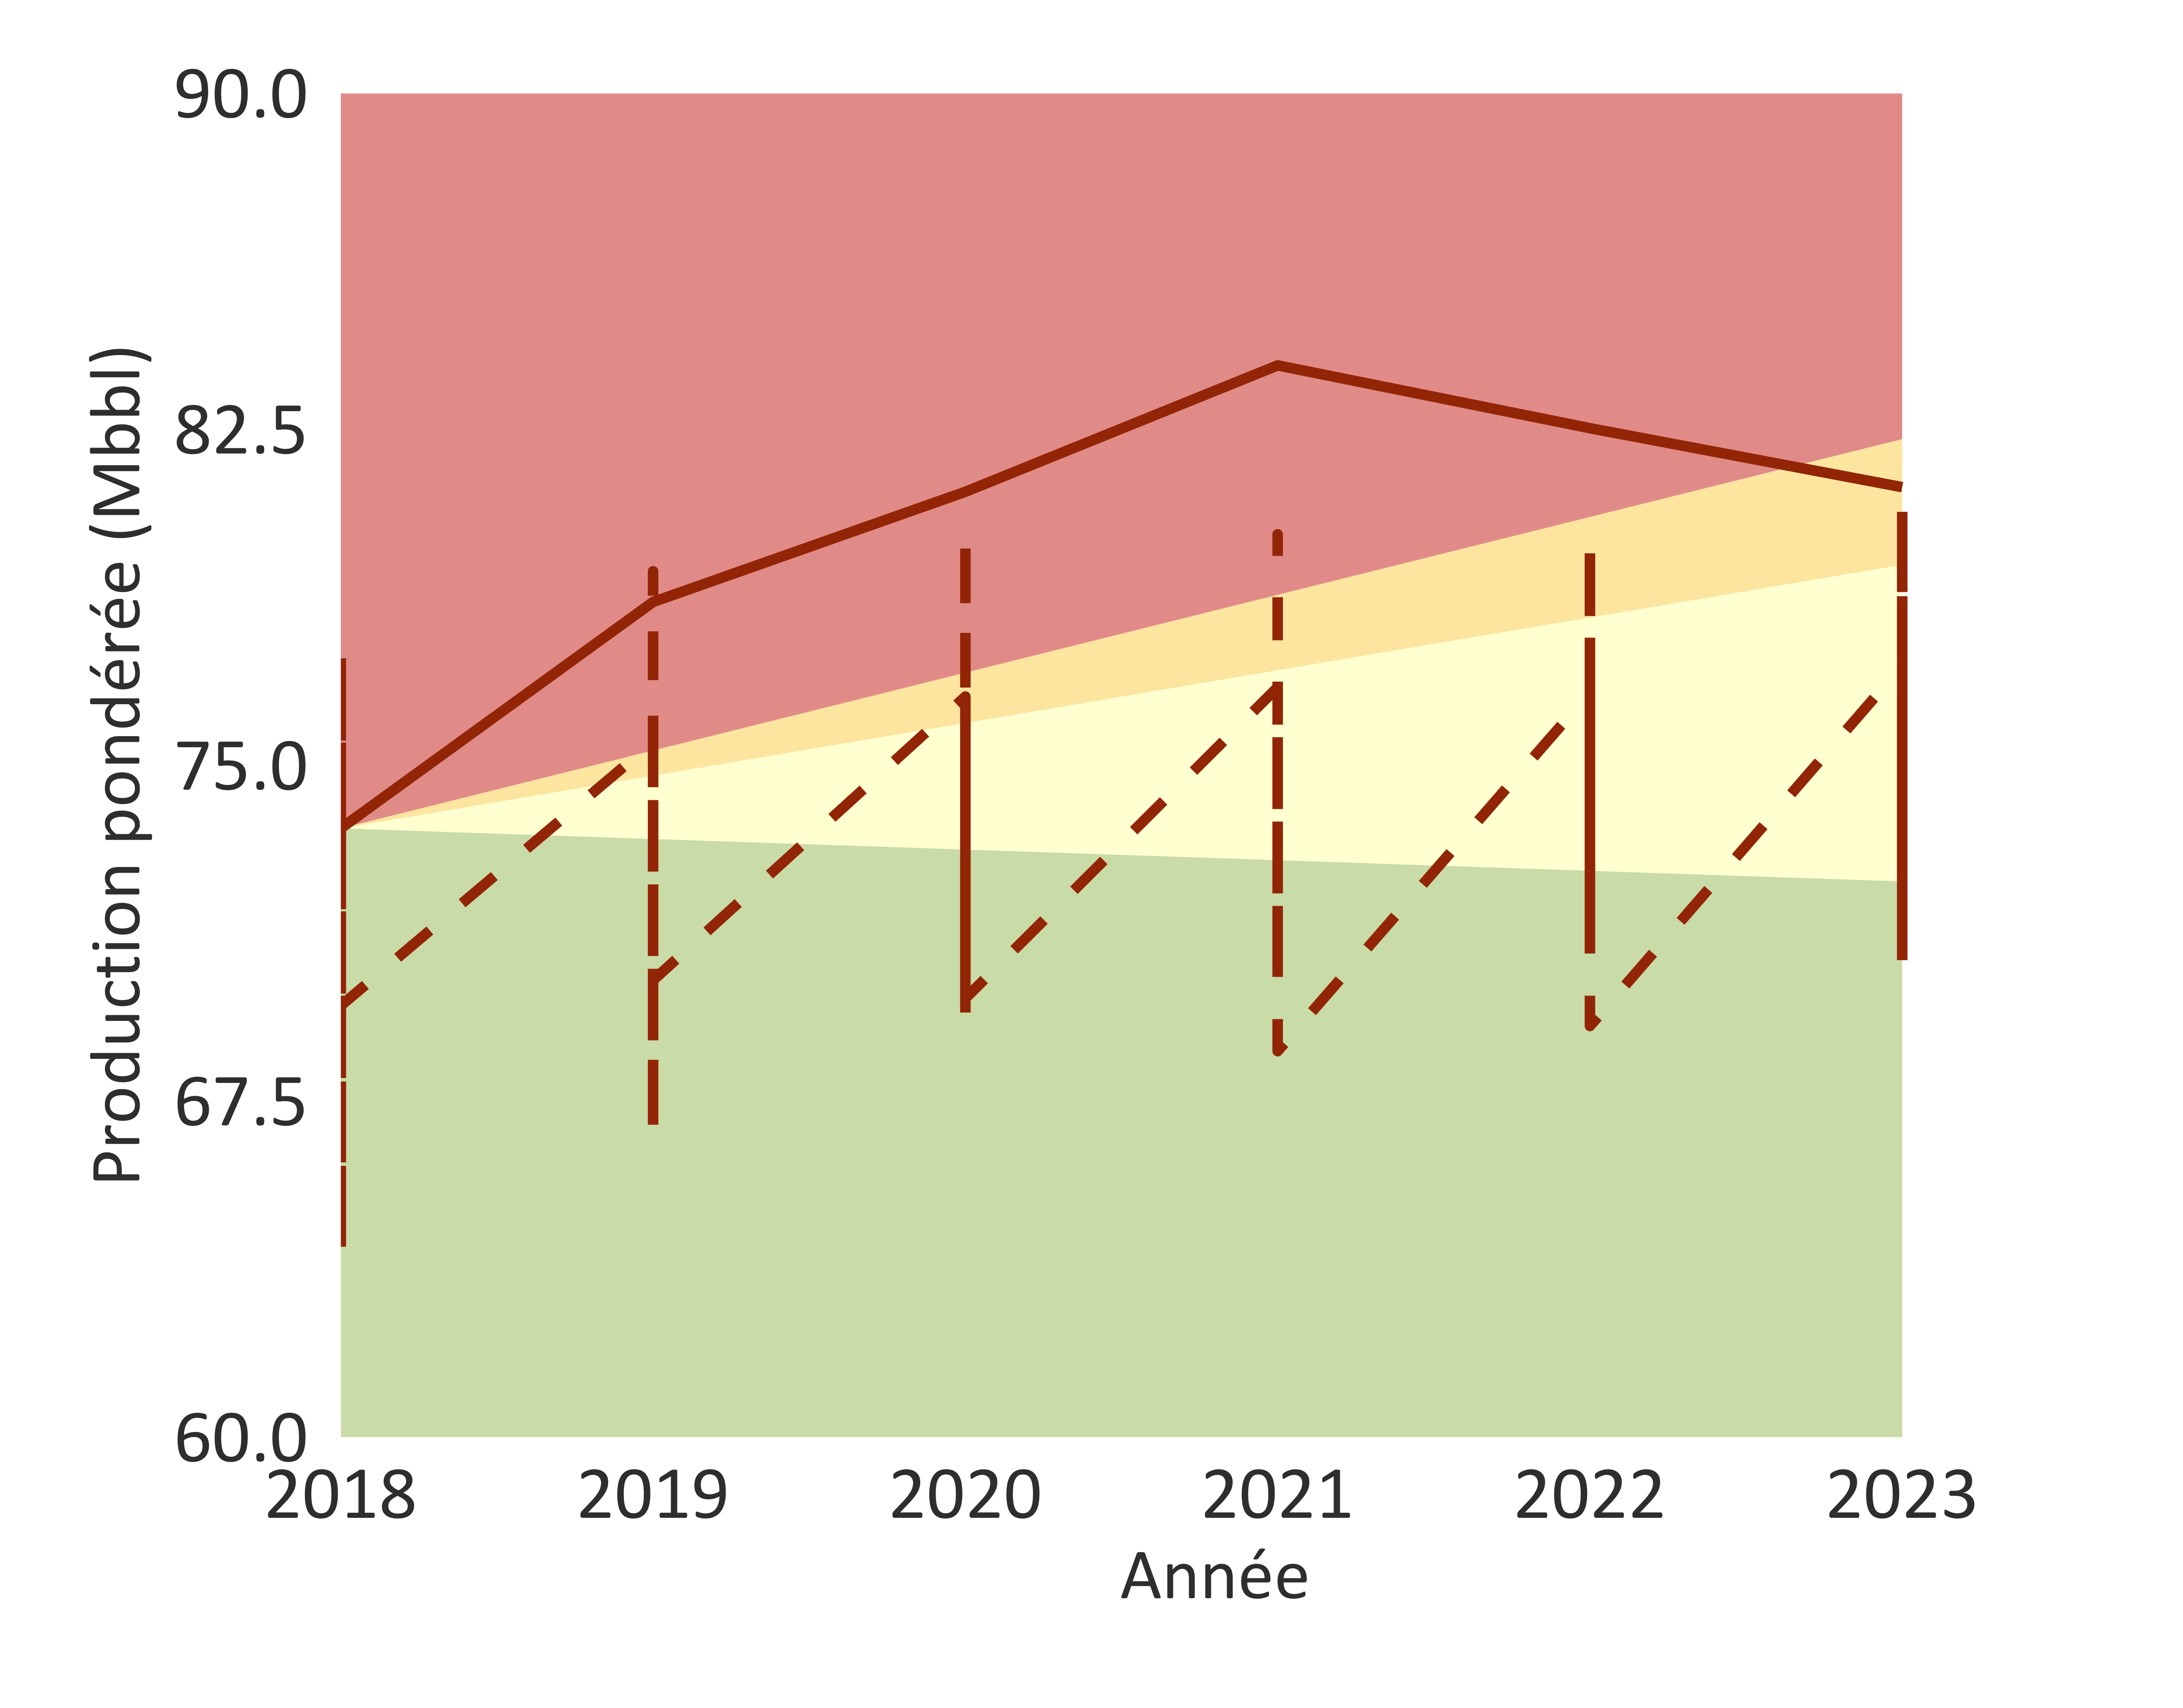
\includegraphics[trim = {0 0cm 0 0},width=1\linewidth]{ReportOutputs/Fig21}
		
	\end{minipage}	
	\hspace{.02\linewidth}
	\begin{minipage}[t]{.49\textwidth}
	\begin{center}
		\textbf{Trajectoire de la production de gaz }
	\end{center}
		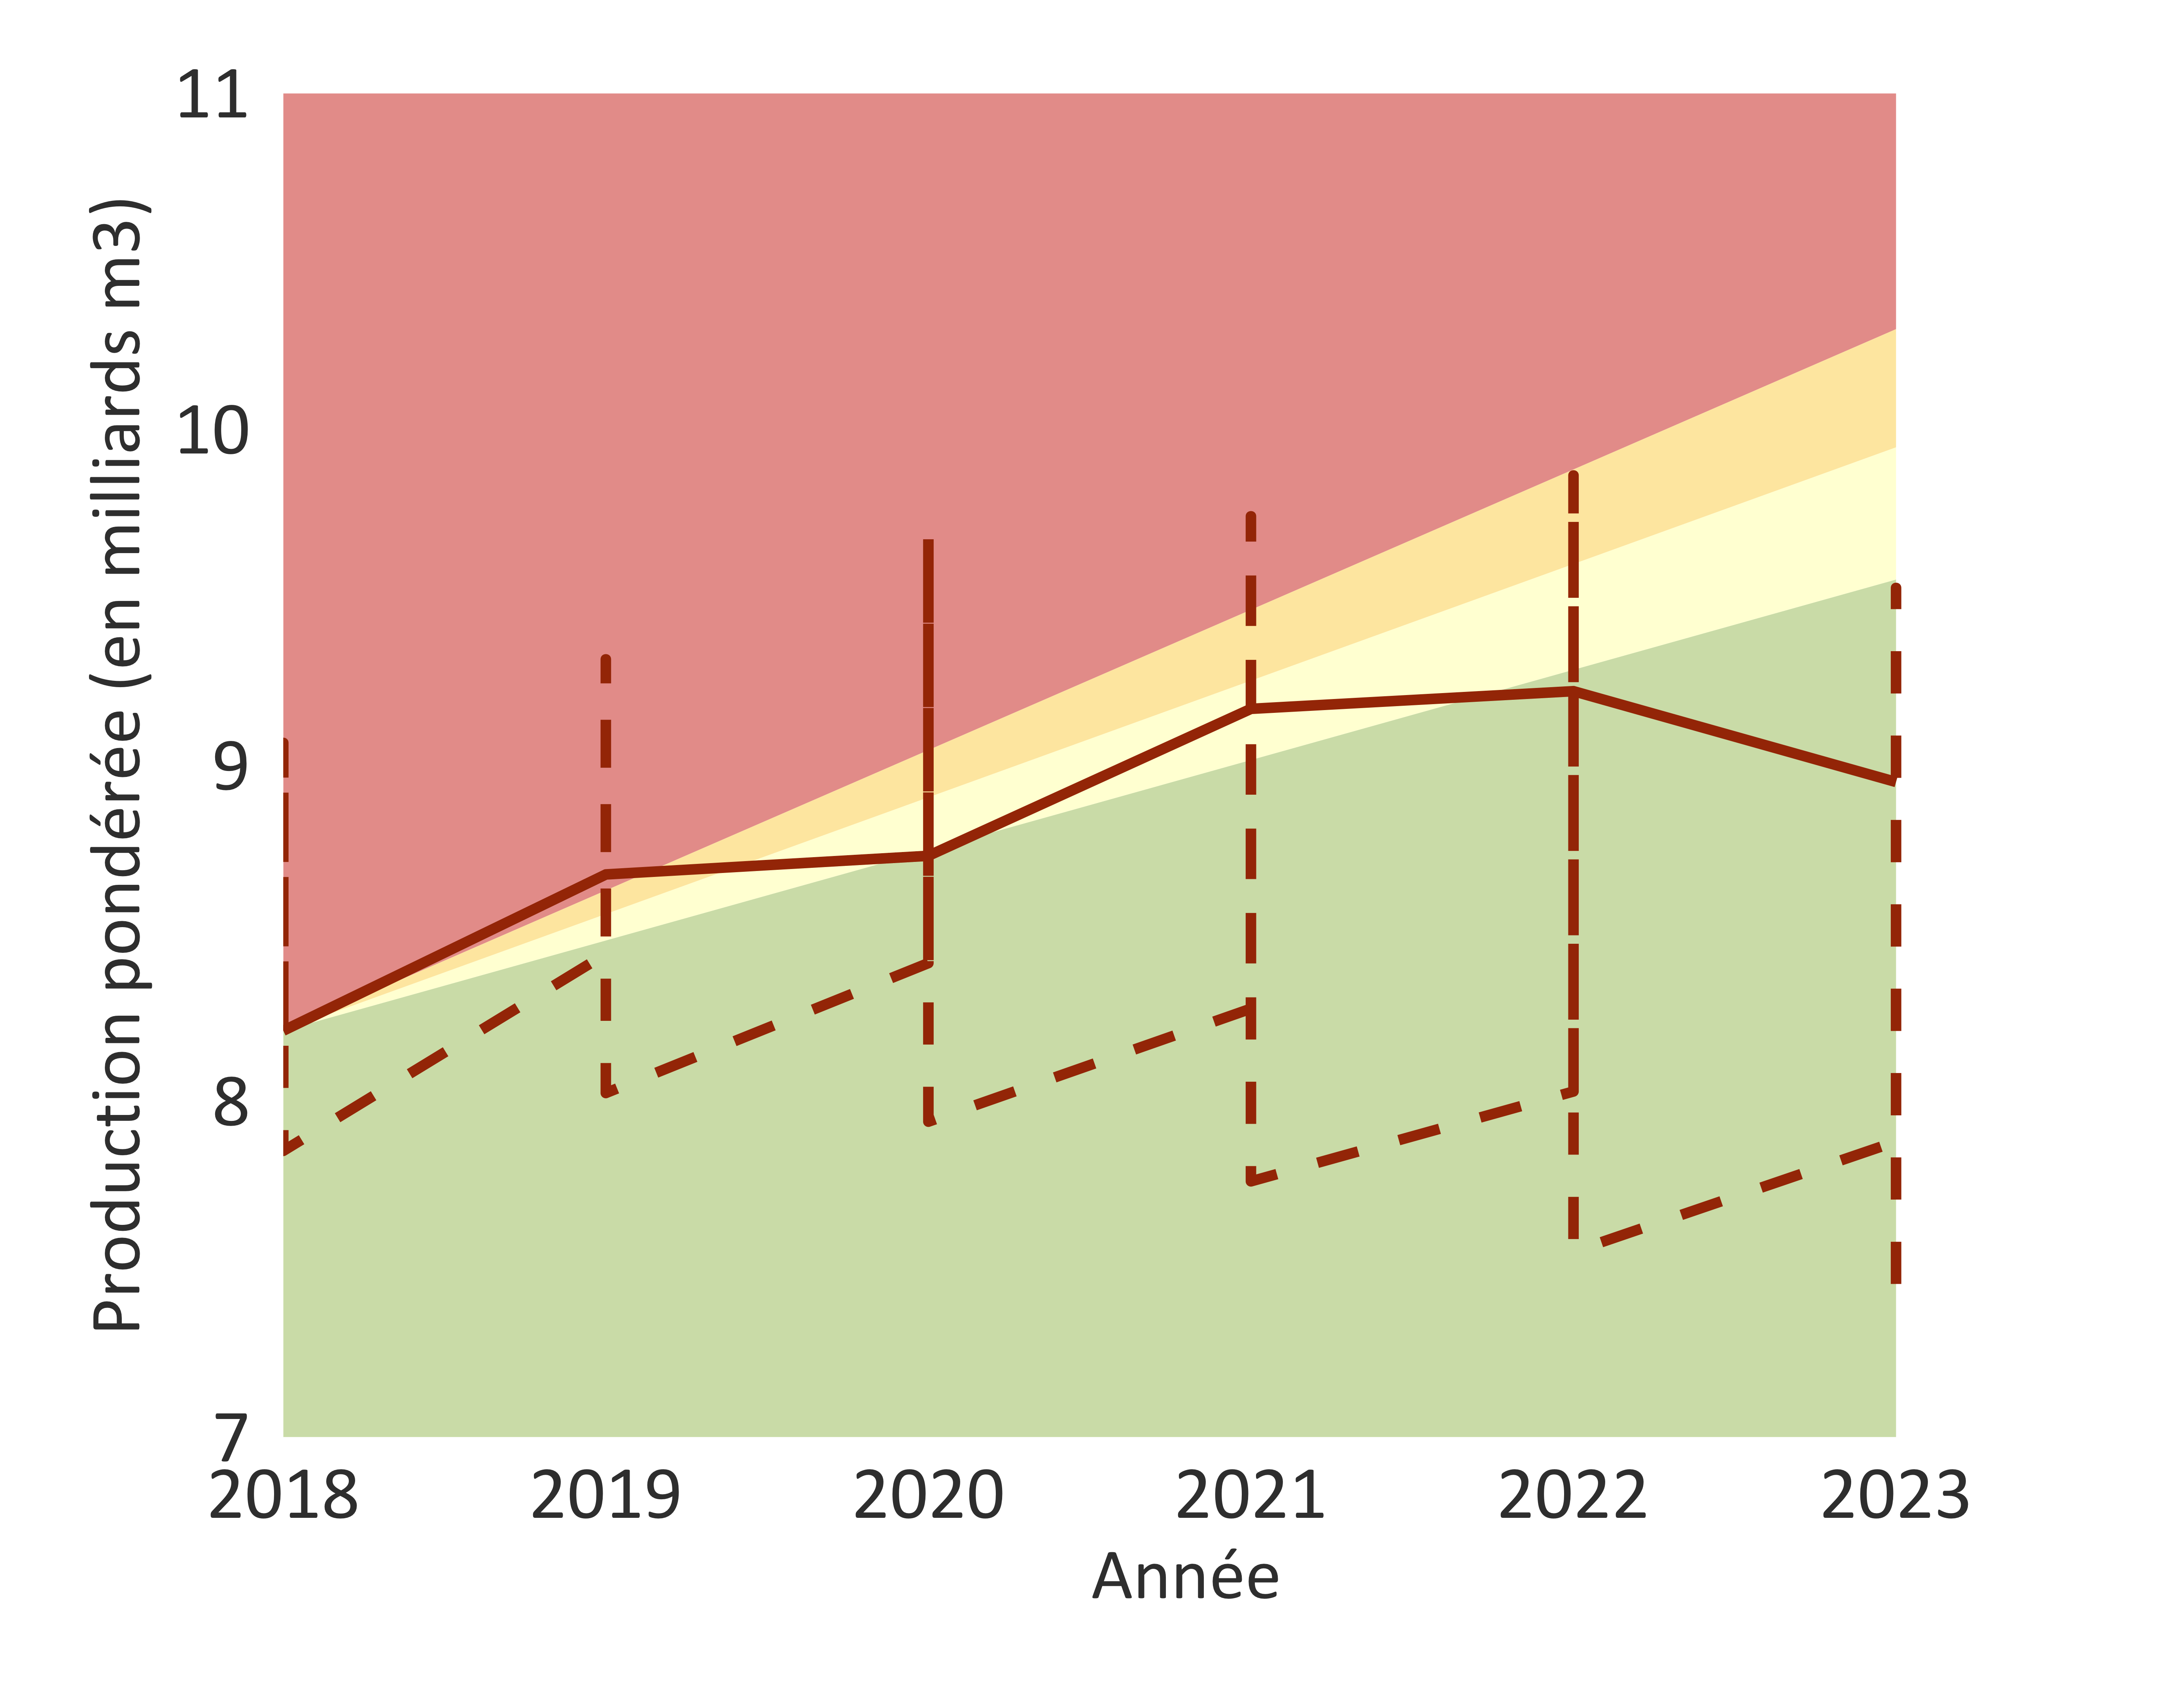
\includegraphics[trim = {0 0cm 0 0},width=1\linewidth]{ReportOutputs/Fig22}
		
	\end{minipage}
	
	
	
	\begin{minipage}[t]{.49\linewidth}
	\begin{center}
		\textbf{Trajectoire de la production de charbon}
	\end{center}
		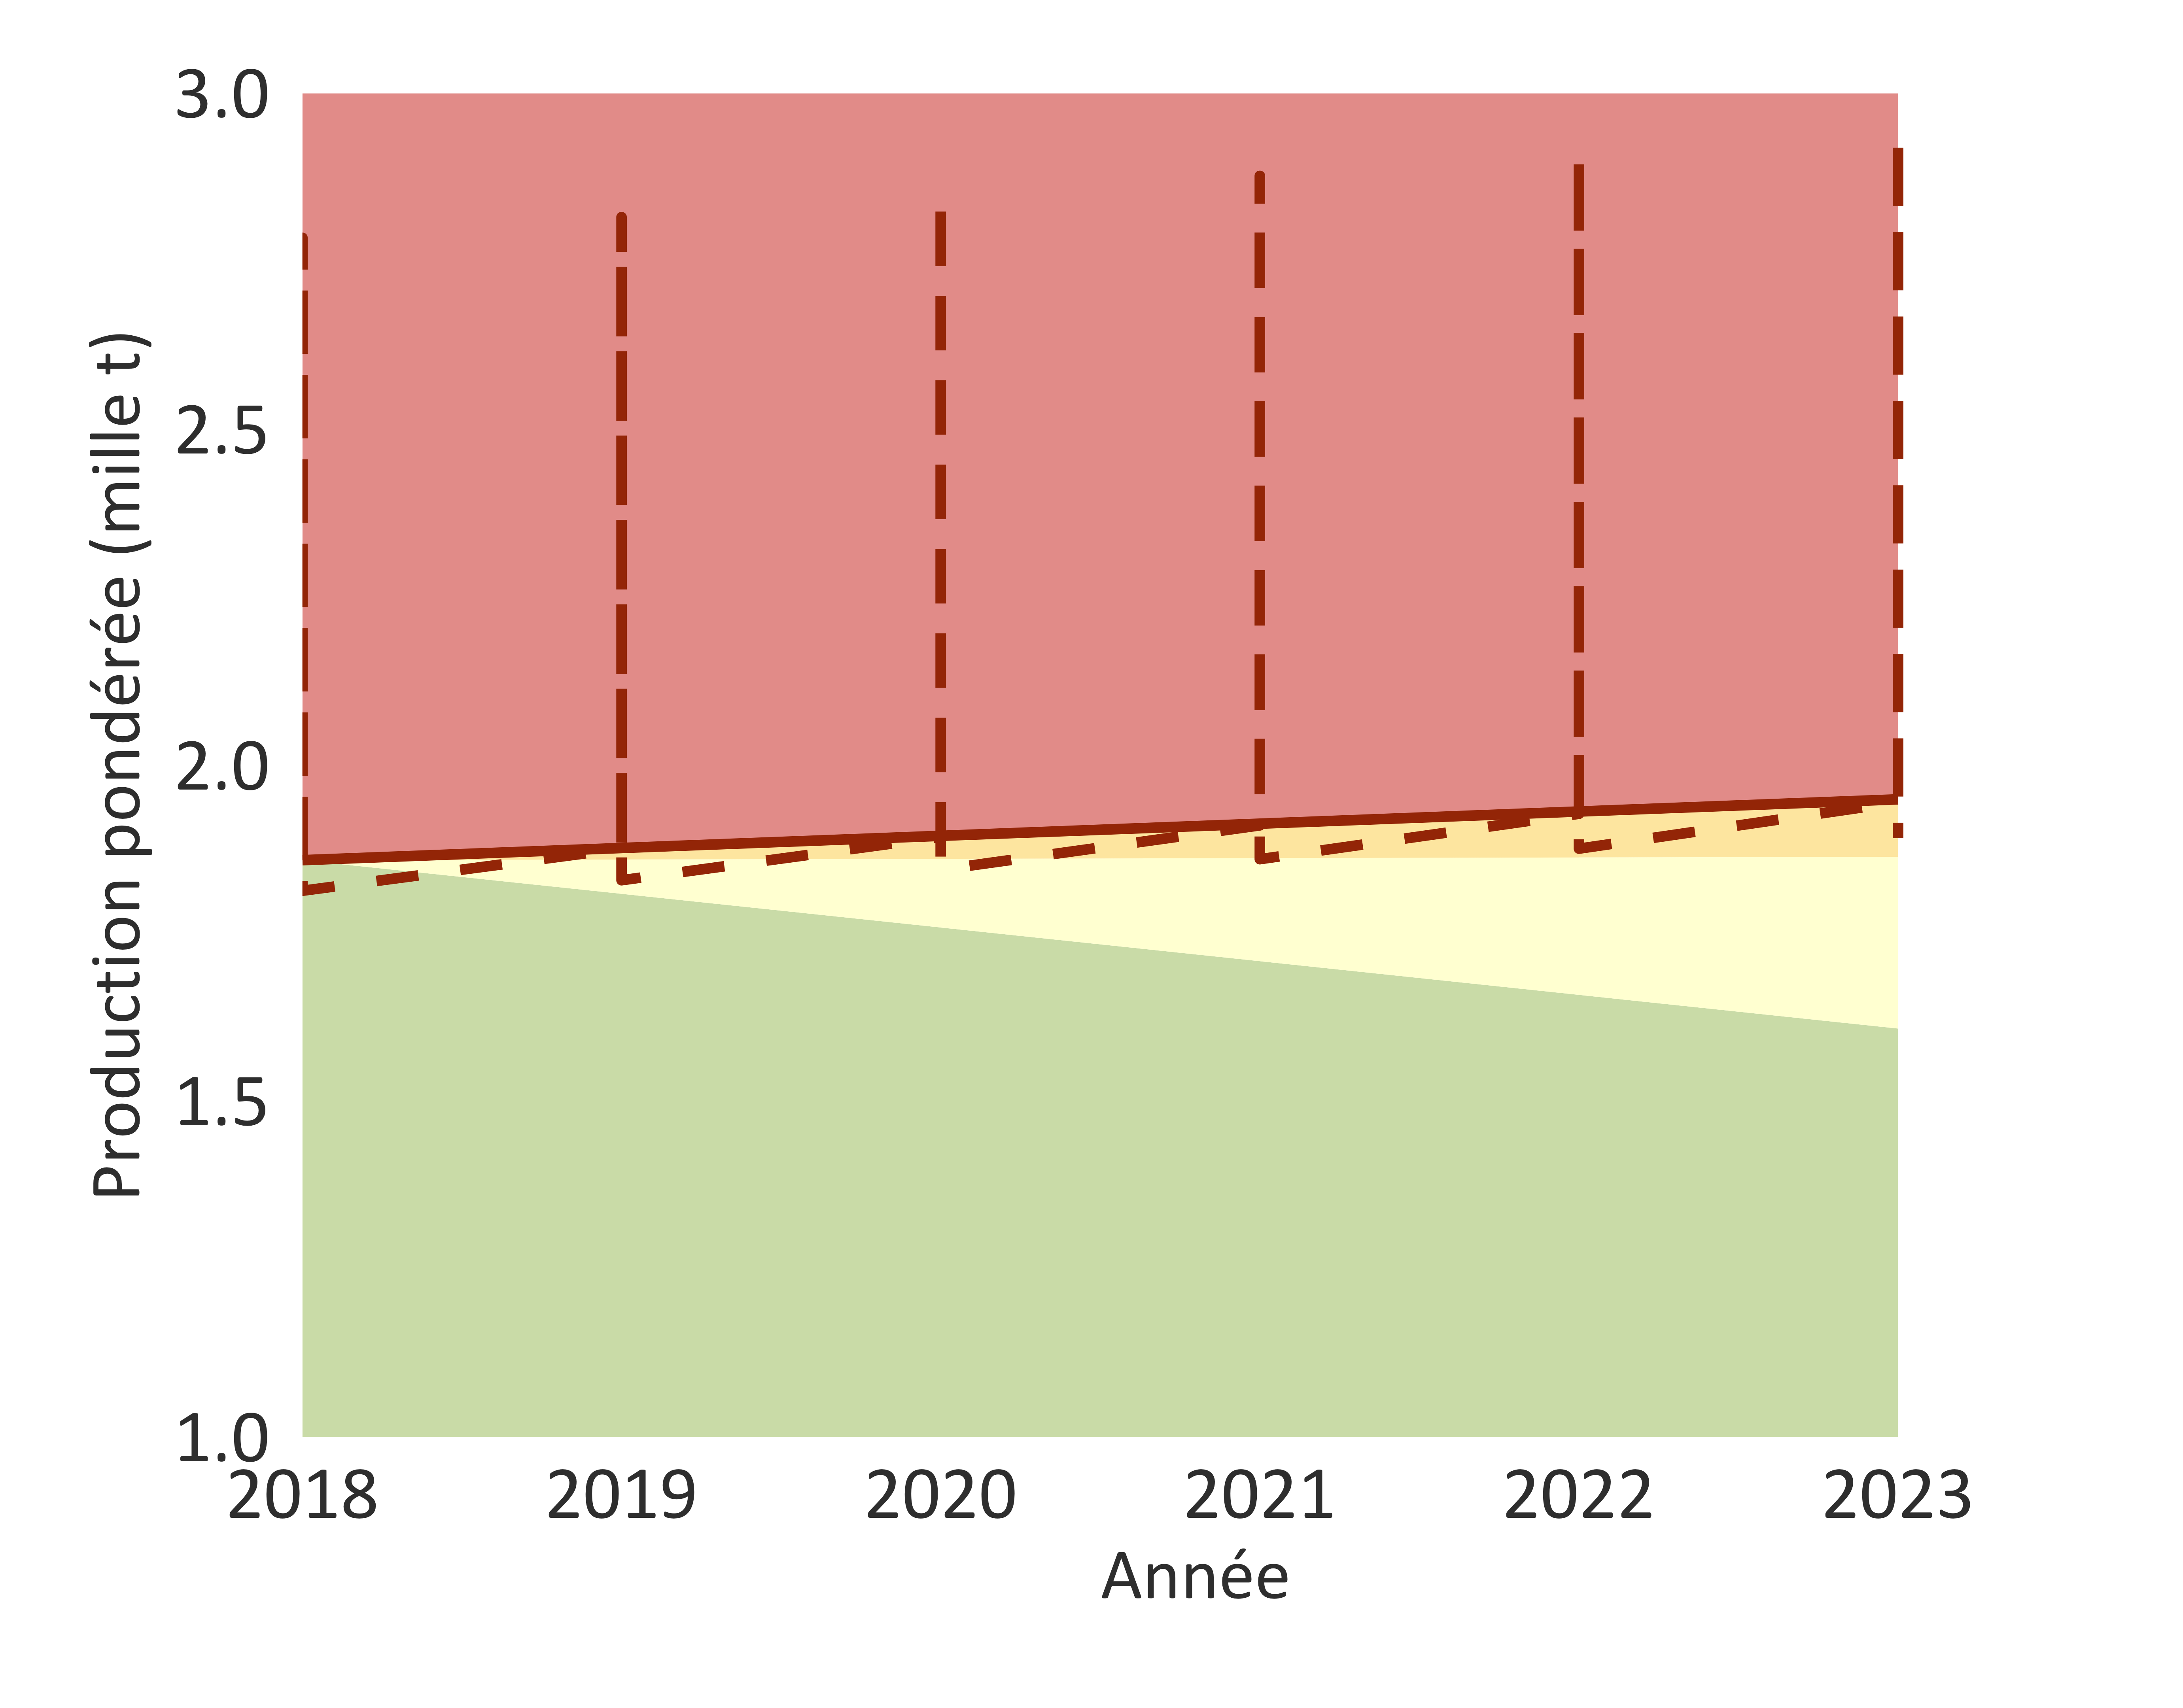
\includegraphics[trim = {0 0cm 0 0},width=1\linewidth]{ReportOutputs/Fig23}
		
	\end{minipage}	
	
	
	\vspace{-.1cm}
	\begin{center}
		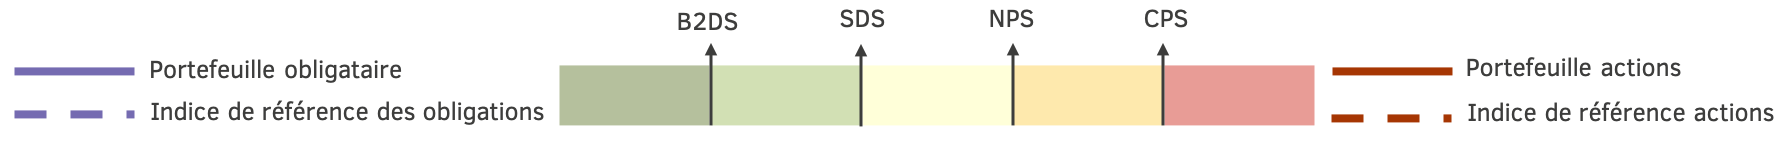
\includegraphics[trim = {0 0cm 0 0},width=1\linewidth]{ReportGraphics/246Legend_FR.png}
	\end{center}
	
	
	\PageFooterThird
	\newpage  
	%FossilFuelSector_EQE 
	%FossilFuelSector_ALLE
	%AutoSector_ALLS
	%AutoSector_CBS
	\section*{} % TRAJECTORY - BONDS - AUTOMOTIVE  
	\HeaderDouble{TENDANCE A 5 ANS - OBLIGATIONS }{AUTOMOBILE}	
	
	\begin{multicols}{2}
		\textbf{Les graphiques ci-dessous illustrent l'alignement du portefeuille d’obligations d’entreprises pour les technologies de production automobiles par rapport aux scénarios de transition de l'AIE: B2DS, SDS, NPS et le marché obligataire.}\\ 
		Pour chaque technologie, la valeur tracée pour le portefeuille (ligne continue) correspond à l'évolution ou la « trajectoire » prévue de la production automobile affectée au portefeuille d’obligations d’entreprises sur les 5 prochaines années.
		Les lignes séparant les zones d'arrière-plan délimitées par couleur représentent la « production cible » du portefeuille pour chaque technologie selon les scénarios de l'AIE. La ligne en pointillés montre la trajectoire prévue de la capacité installée pour le marché obligataire pour chaque technologie, mise à l'échelle du portefeuille, pour faciliter la comparaison.
		                  
		
	\end{multicols}		

	
	\begin{minipage}[t]{.49\linewidth}
		\begin{center}
		\textbf{Trajectoire de la production des voitures à combustion}
	  \end{center}
		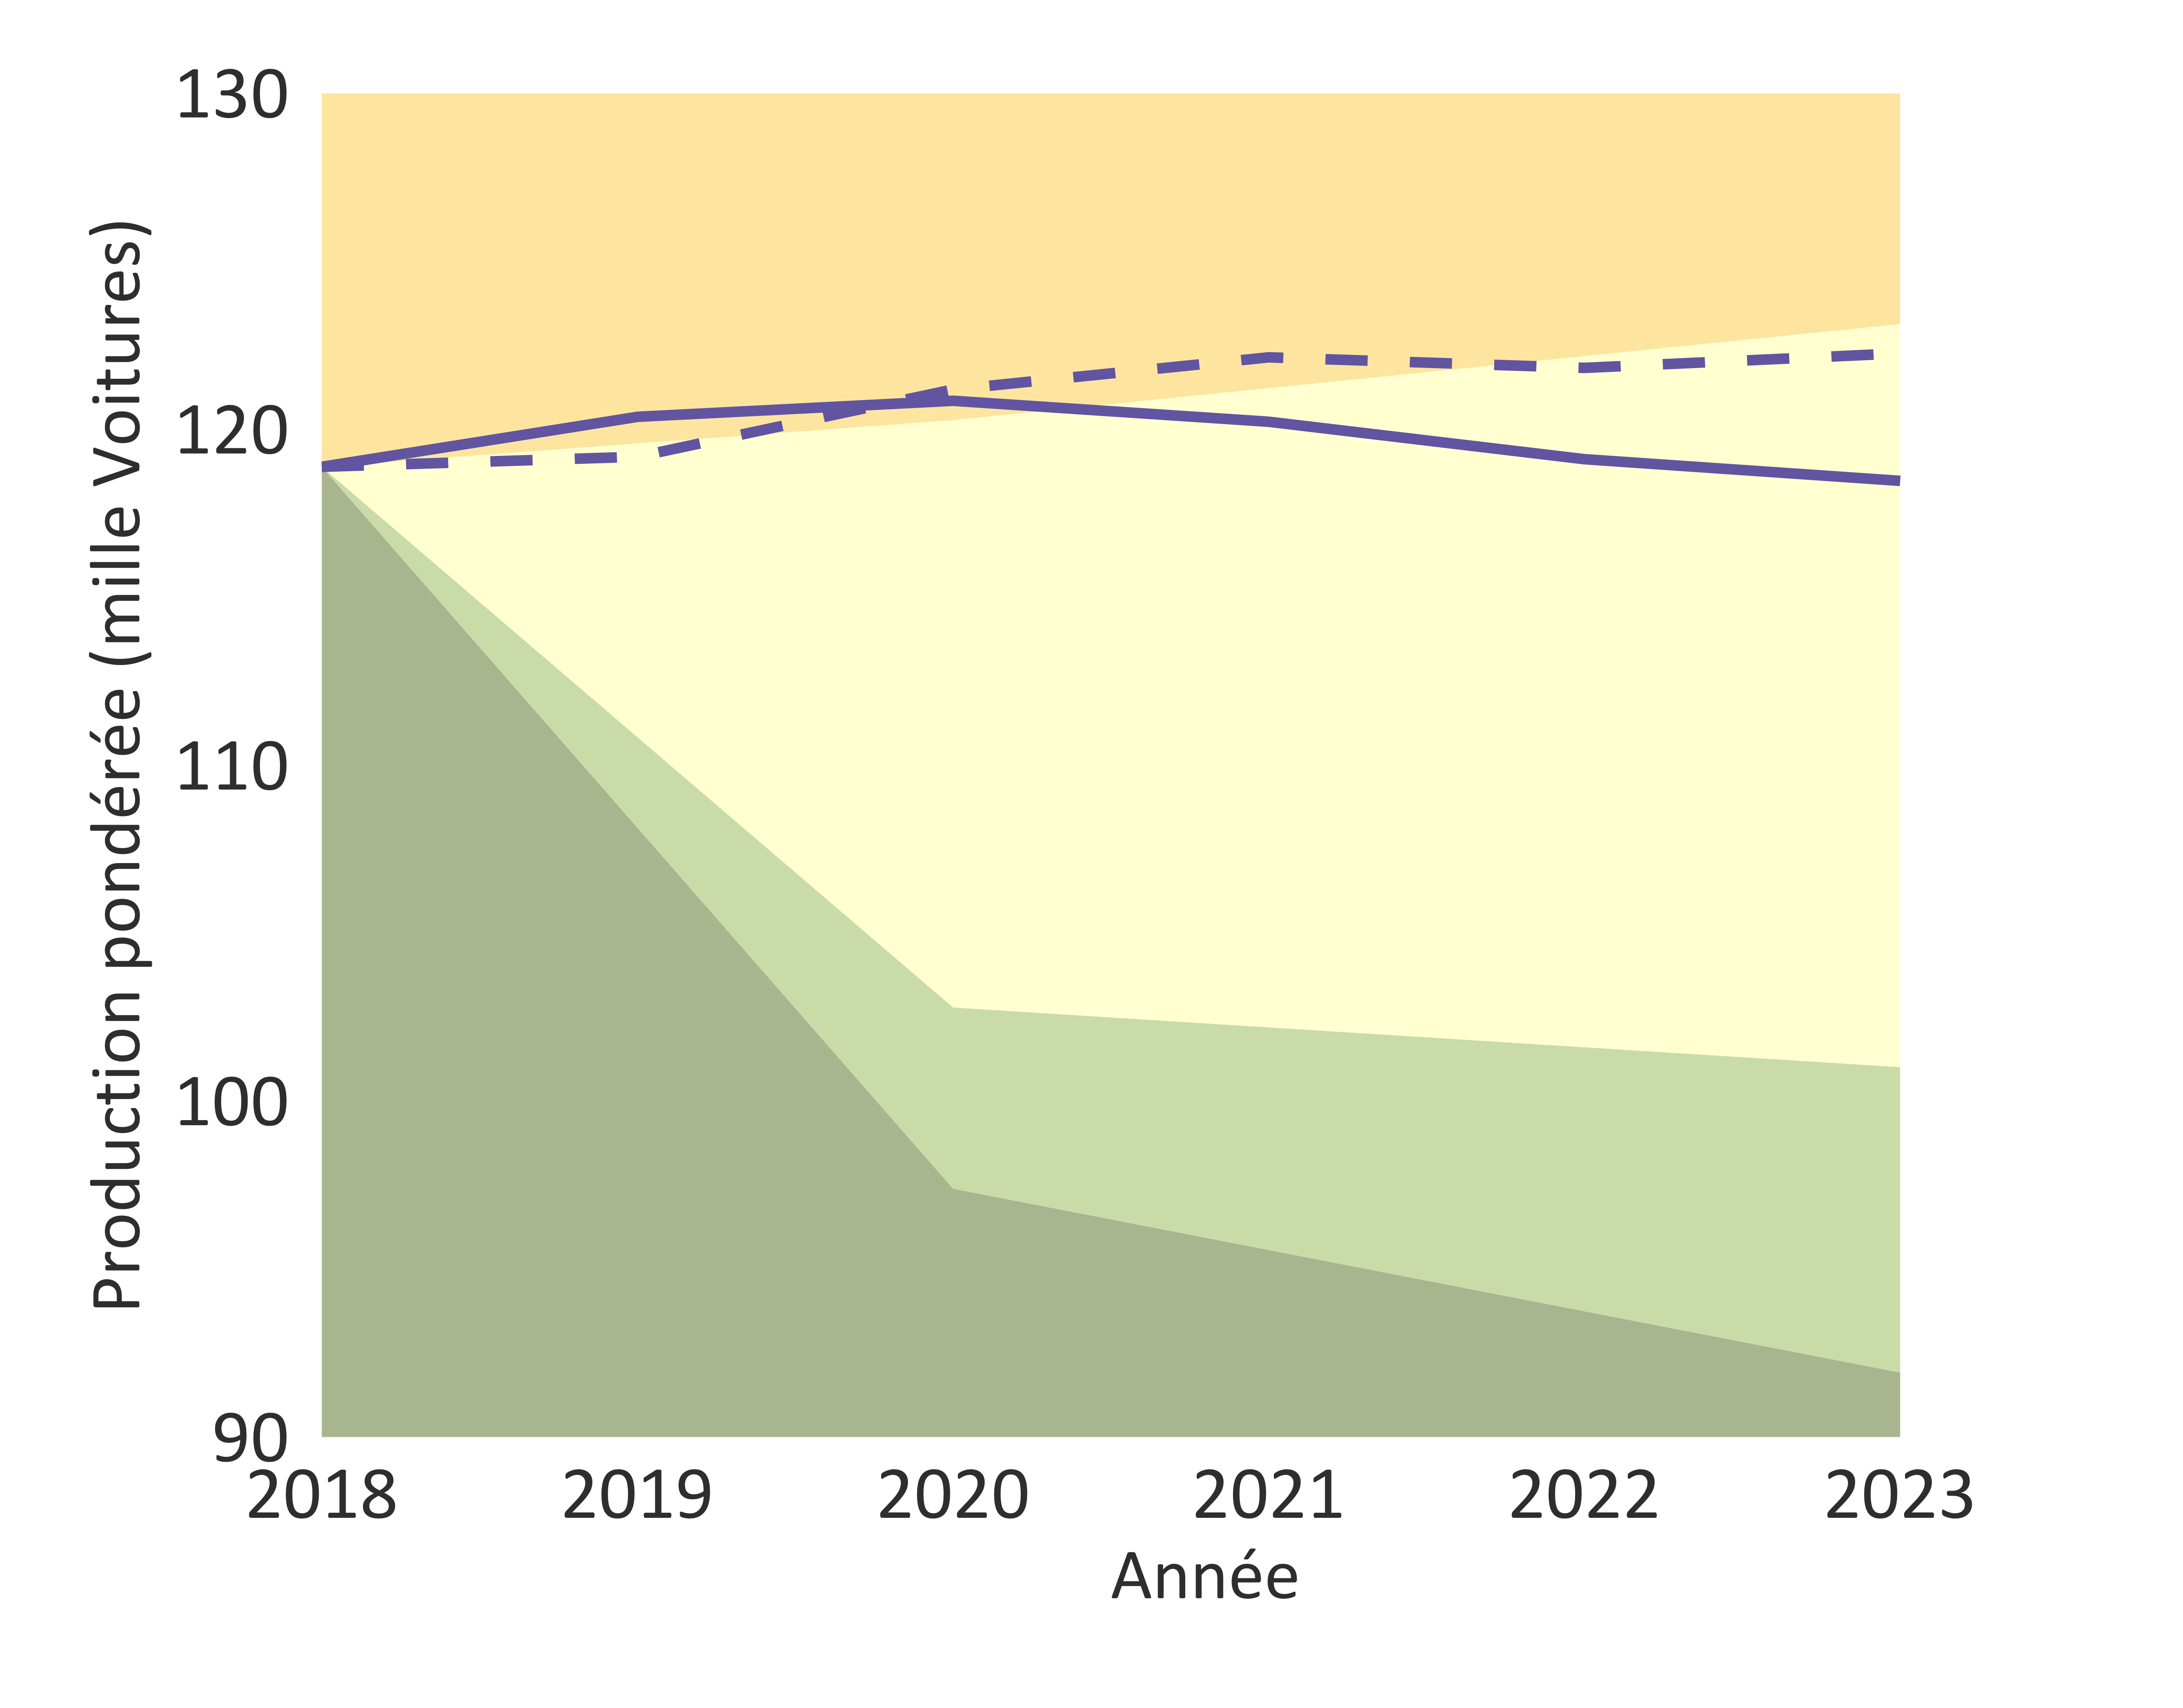
\includegraphics[trim = {0 0cm 0 0},width=1\linewidth]{ReportOutputs/Fig14}
		
	\end{minipage}	
	\hspace{.02\linewidth}
	\begin{minipage}[t]{.49\textwidth}
		\begin{center}
		\textbf{Trajectoire de la production des voitures électriques}
	  \end{center}
		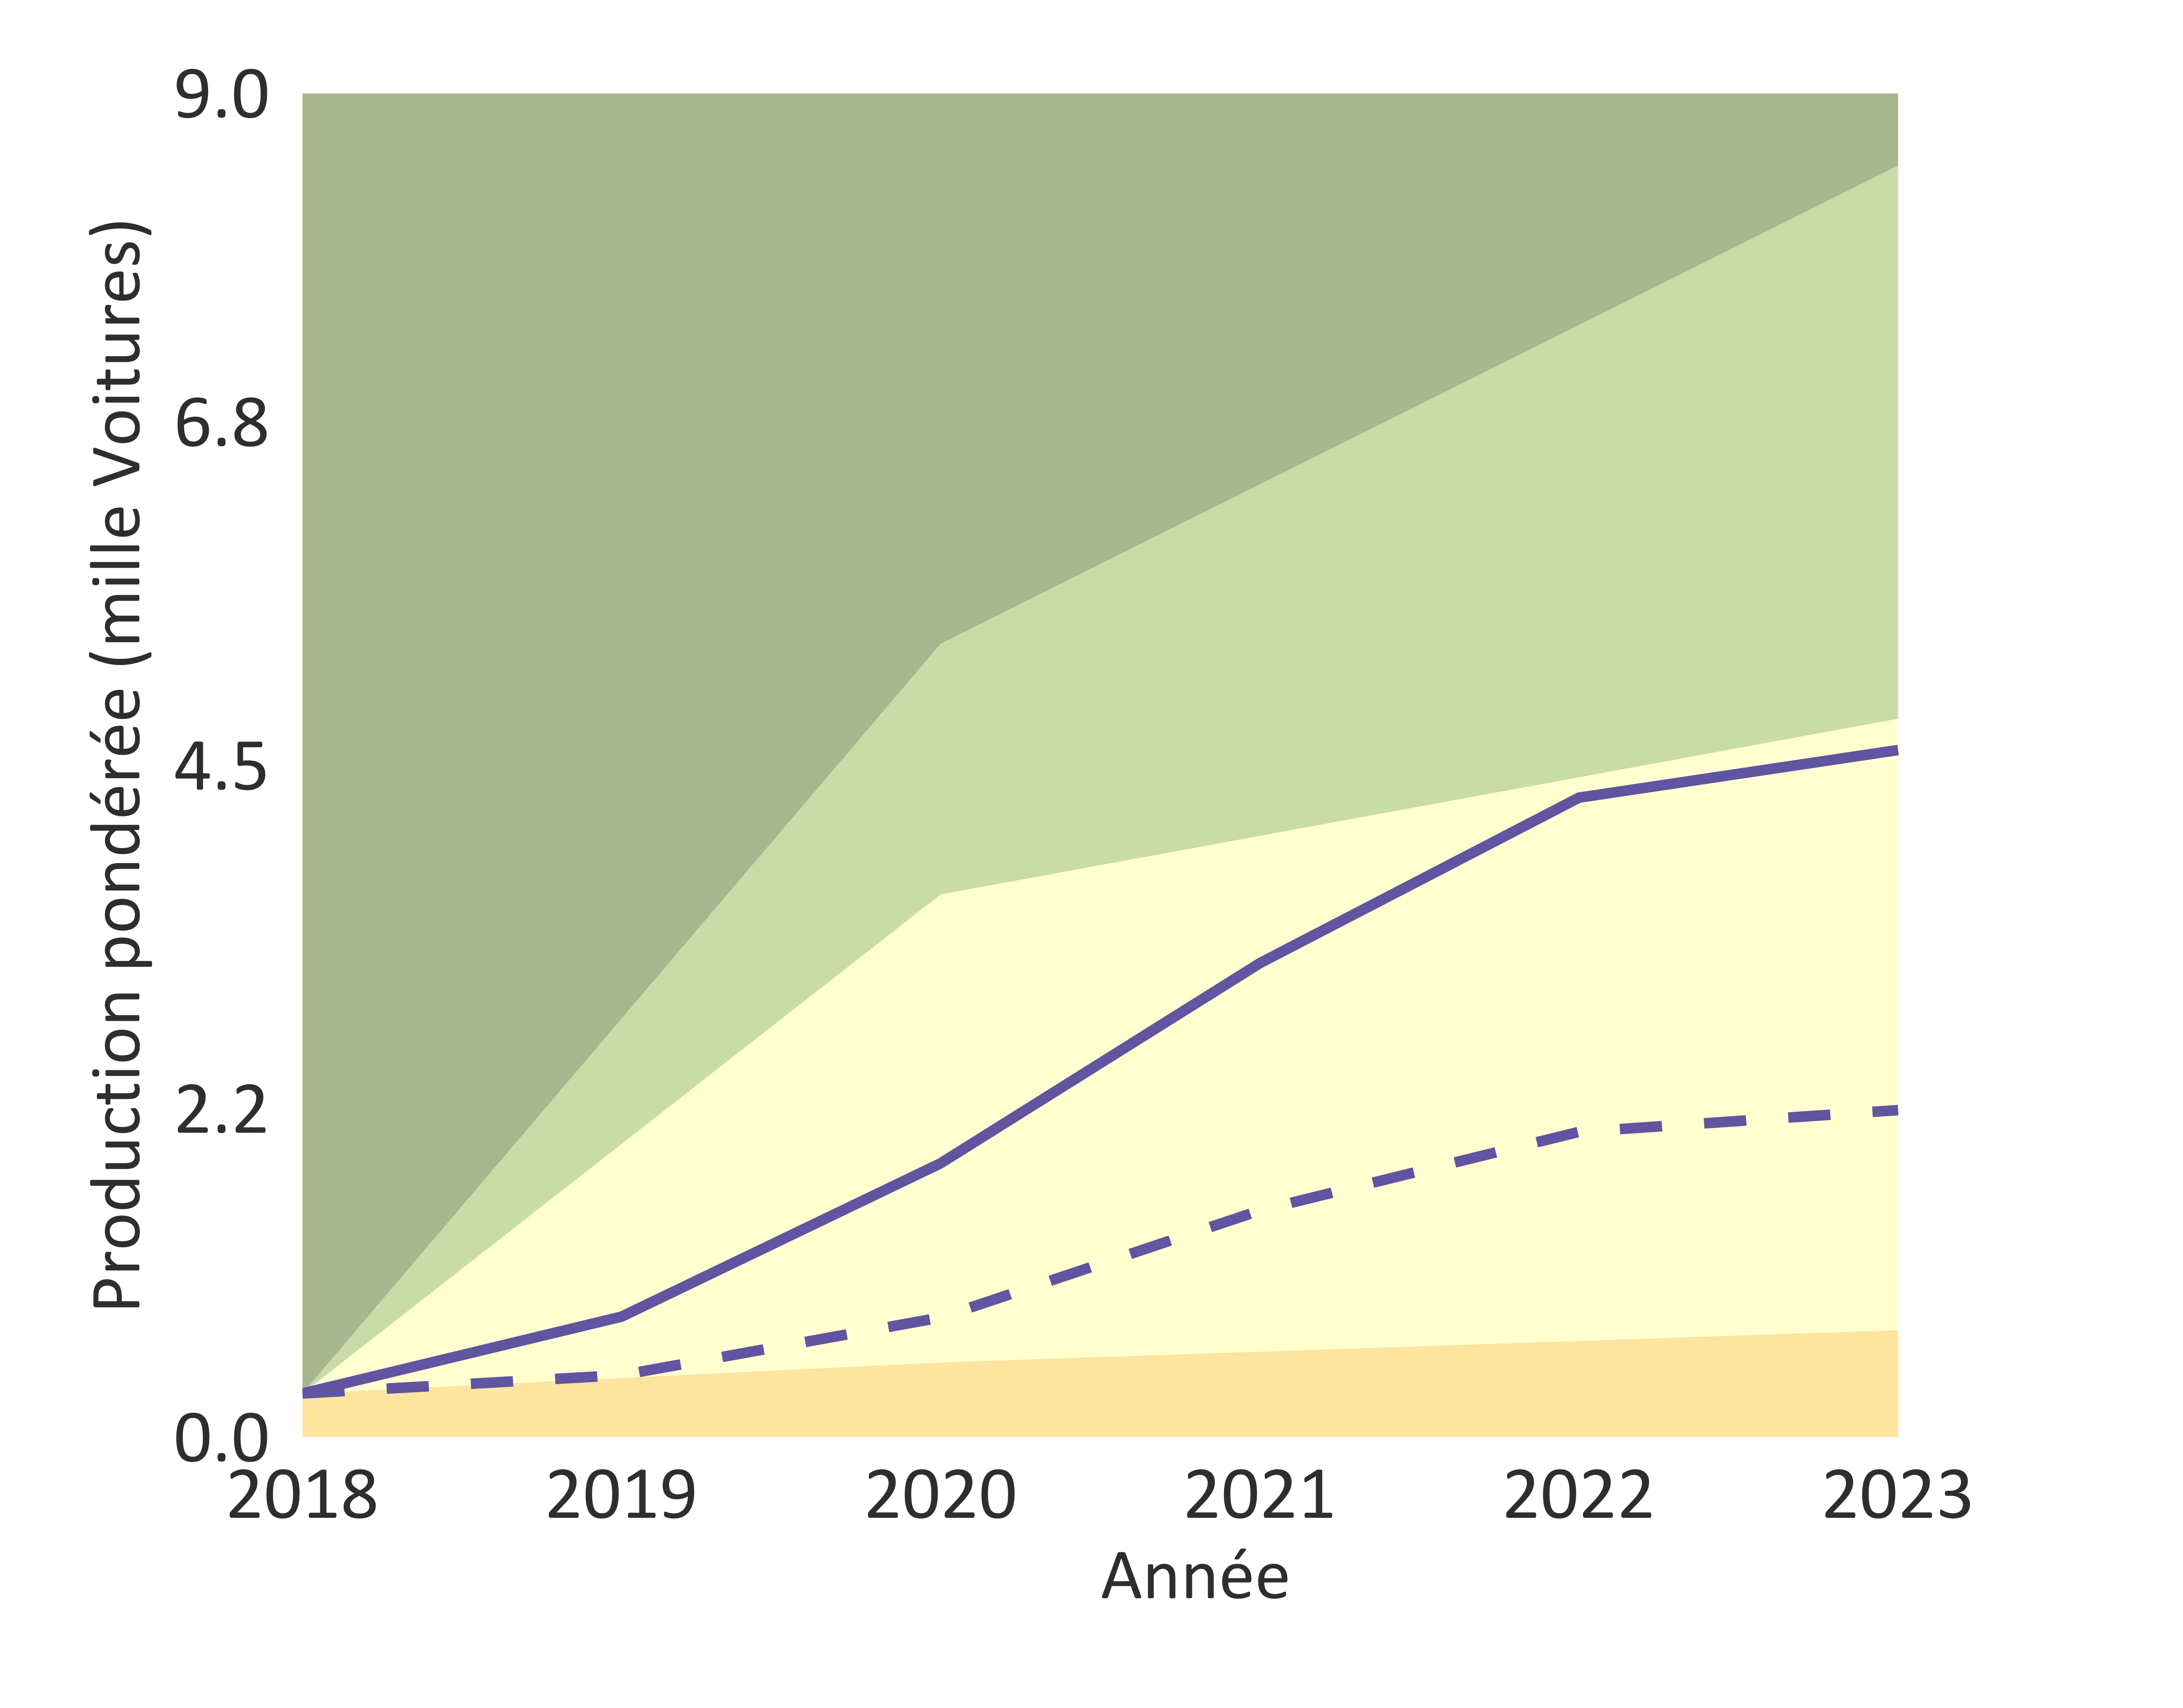
\includegraphics[trim = {0 0cm 0 0},width=1\linewidth]{ReportOutputs/Fig15}
		
	\end{minipage}	

	\begin{minipage}[t]{.49\textwidth}
		\begin{center}
		\textbf{Trajectoire de la production des voitures hybrides}
	 \end{center}
		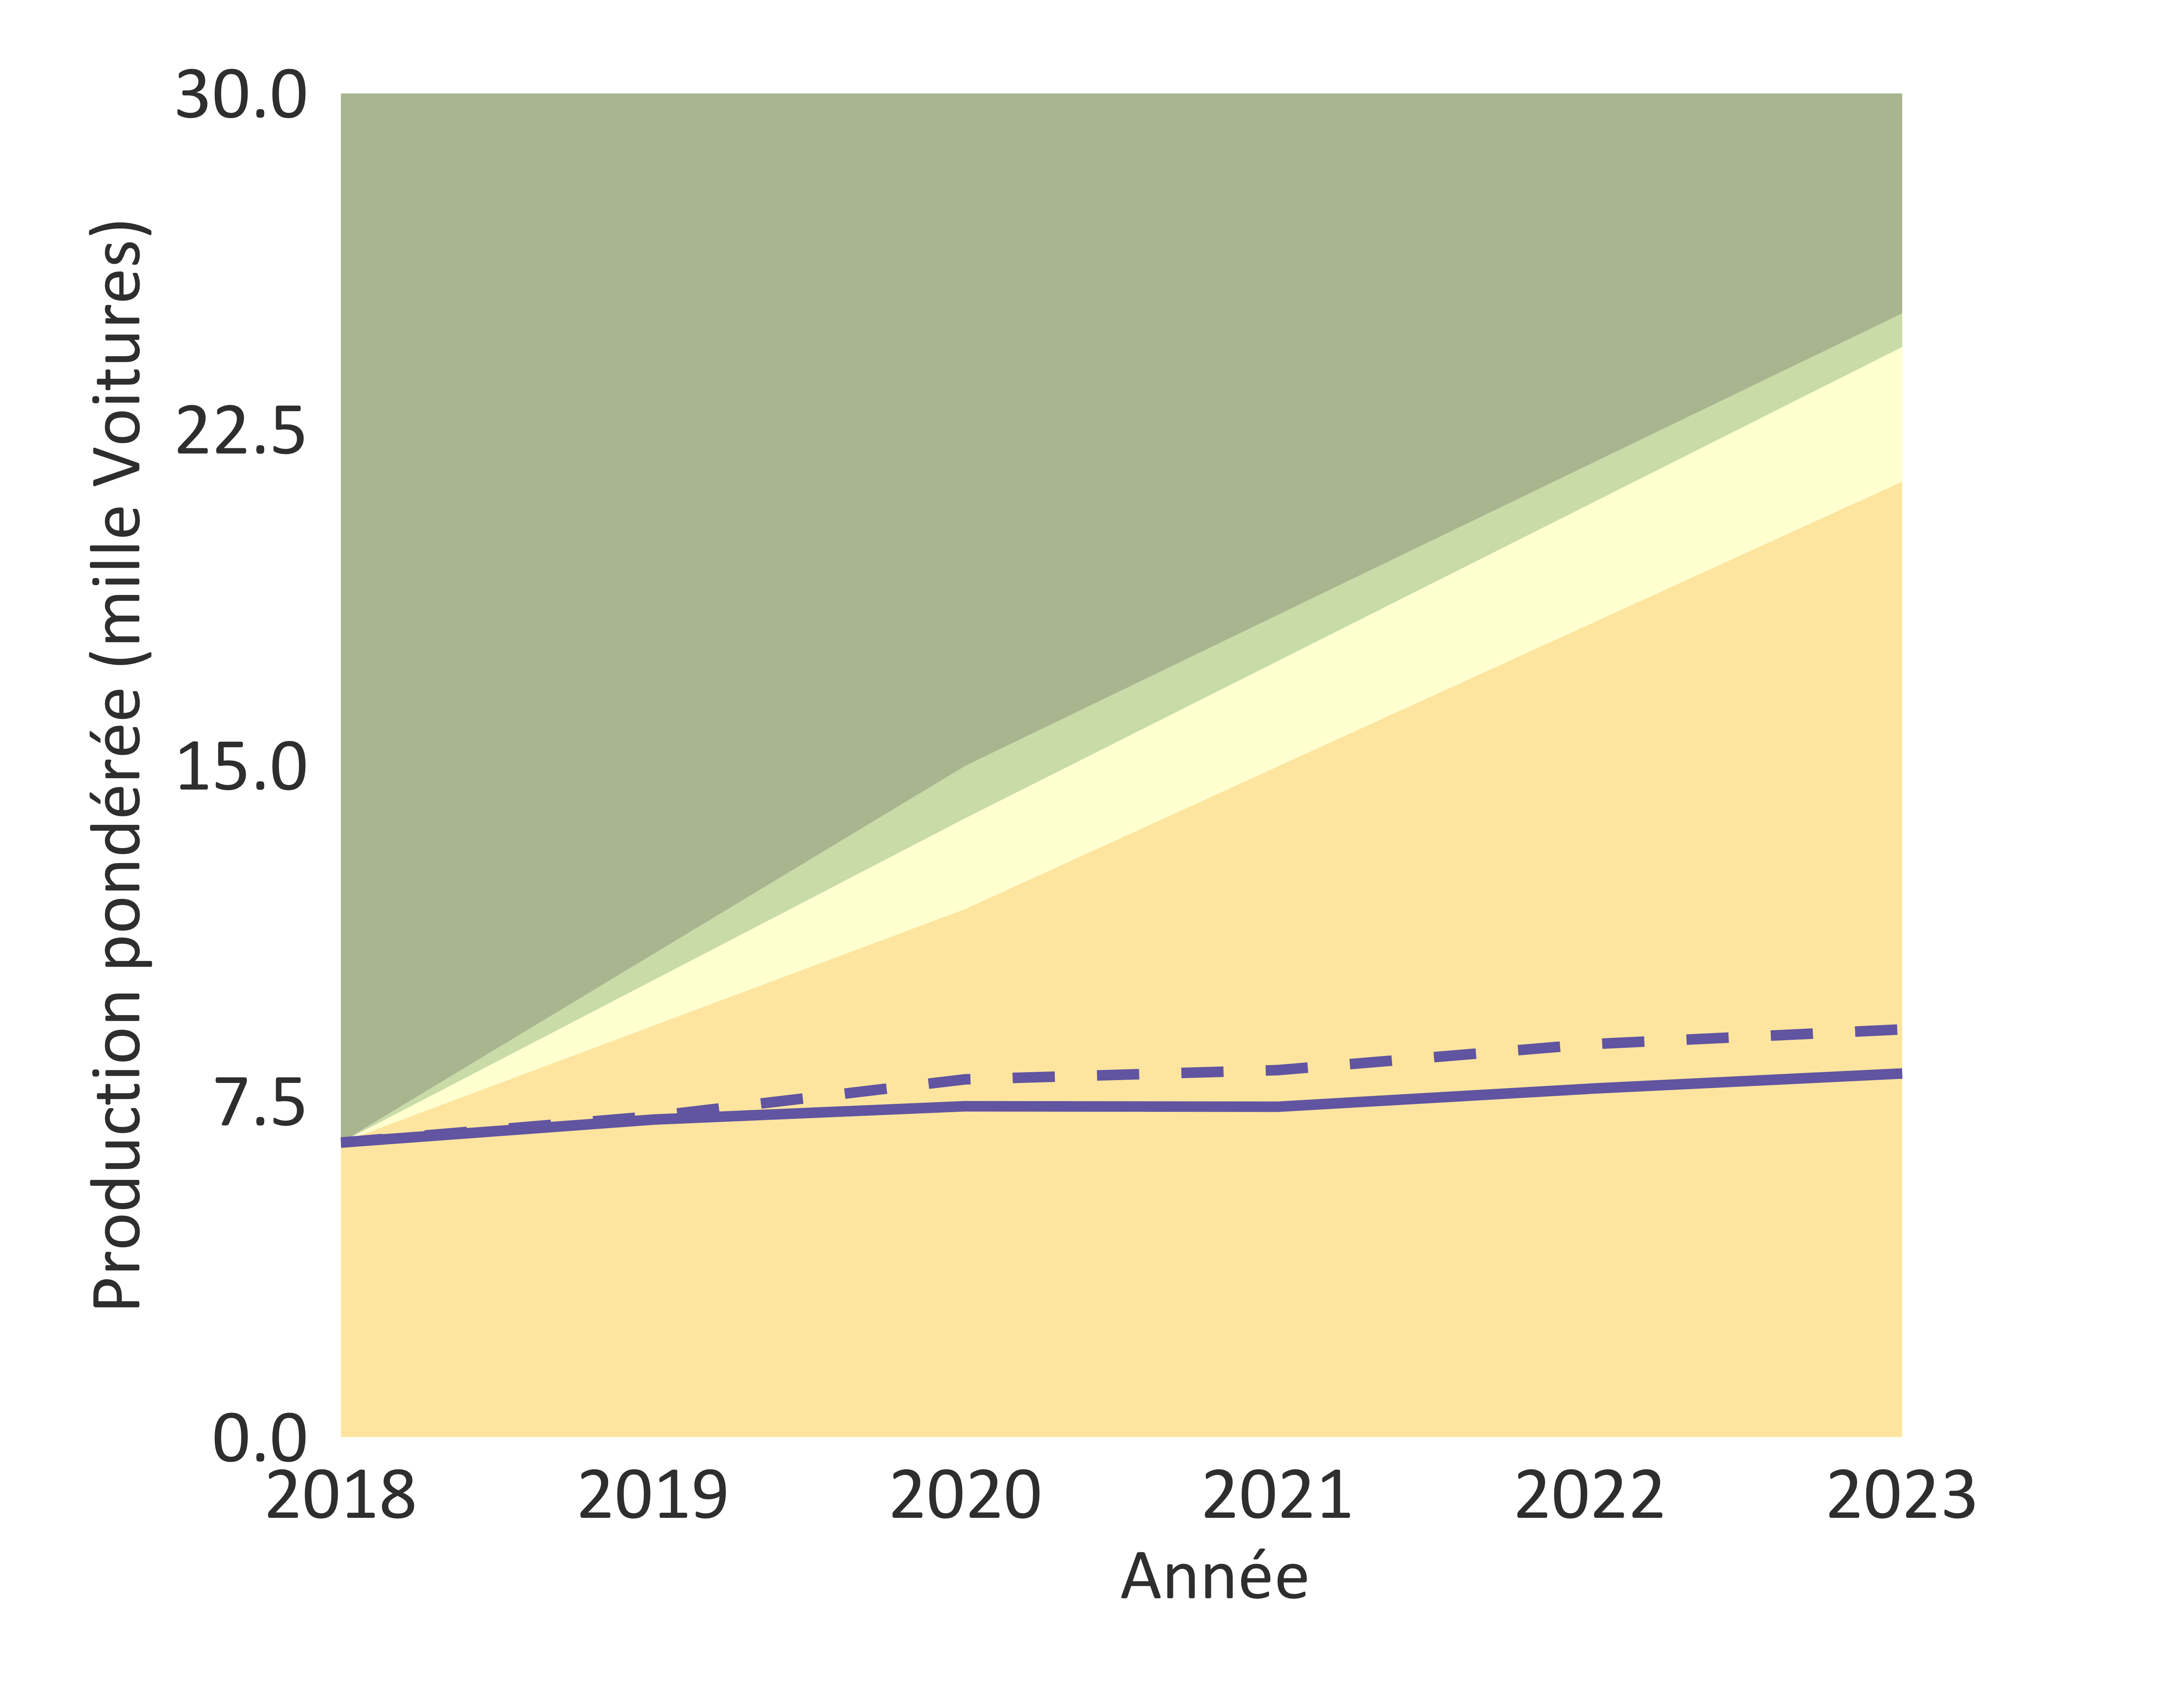
\includegraphics[trim = {0 0cm 0 0},width=1\linewidth]{ReportOutputs/Fig16}
	
	\end{minipage}		
	
	\vspace{-.1cm}
	\begin{center}
		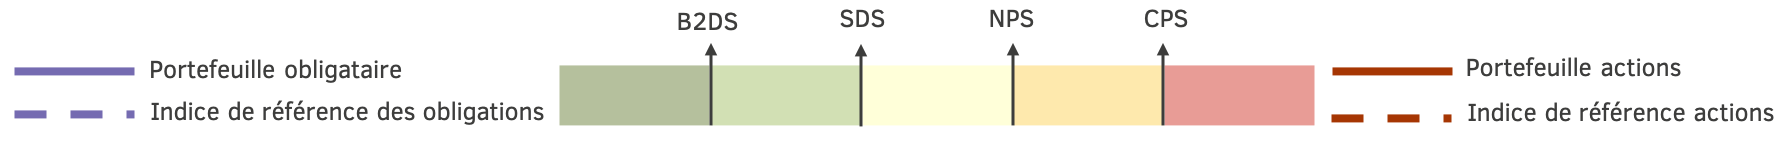
\includegraphics[trim = {0 0cm 0 0},width=1\linewidth]{ReportGraphics/246Legend_FR.png}
	\end{center}
	
	
	\PageFooterThird
	\newpage 
	%AutoSector_CBE 
	%AutoSector_EQS	
	\section*{} % TRAJECTORY - EQUITY - FOSSIL FUELS AND AUTOMOTIVE 
		\HeaderDouble{TENDANCE A 5 ANS - ACTIONS}{AUTOMOBILE}	
	
	\begin{multicols}{2}
		\textbf{Les graphiques ci-dessous illustrent l'alignement du portefeuille actions pour les différentes technologies sélectionnées par rapport aux scénarios de transition de l'AIE: B2DS, SDS, NPS  et l´indice de référence actions.}\\
		Pour chaque technologie, la valeur tracée pour le portefeuille (ligne continue) correspond à l'évolution estimée ou la « trajectoire » de la capacité installée allouée au portefeuille actions sur les 5 prochaines années.
		Les lignes séparant les zones d'arrière-plan délimitées par couleur représentent la « production cible » du portefeuille pour chaque technologie selon les scénarios de l'AIE. La ligne en pointillés montre la trajectoire prévue de la capacité installée pour chaque technologie pour l´indice de référence actions, mise à l'échelle du portefeuille, pour faciliter la comparaison.
		                    
		
	\end{multicols}		
	
	
	\begin{minipage}[t]{.49\linewidth}
	\begin{center}
		\textbf{Trajectoire de la production des voitures à combustion}
	\end{center}
		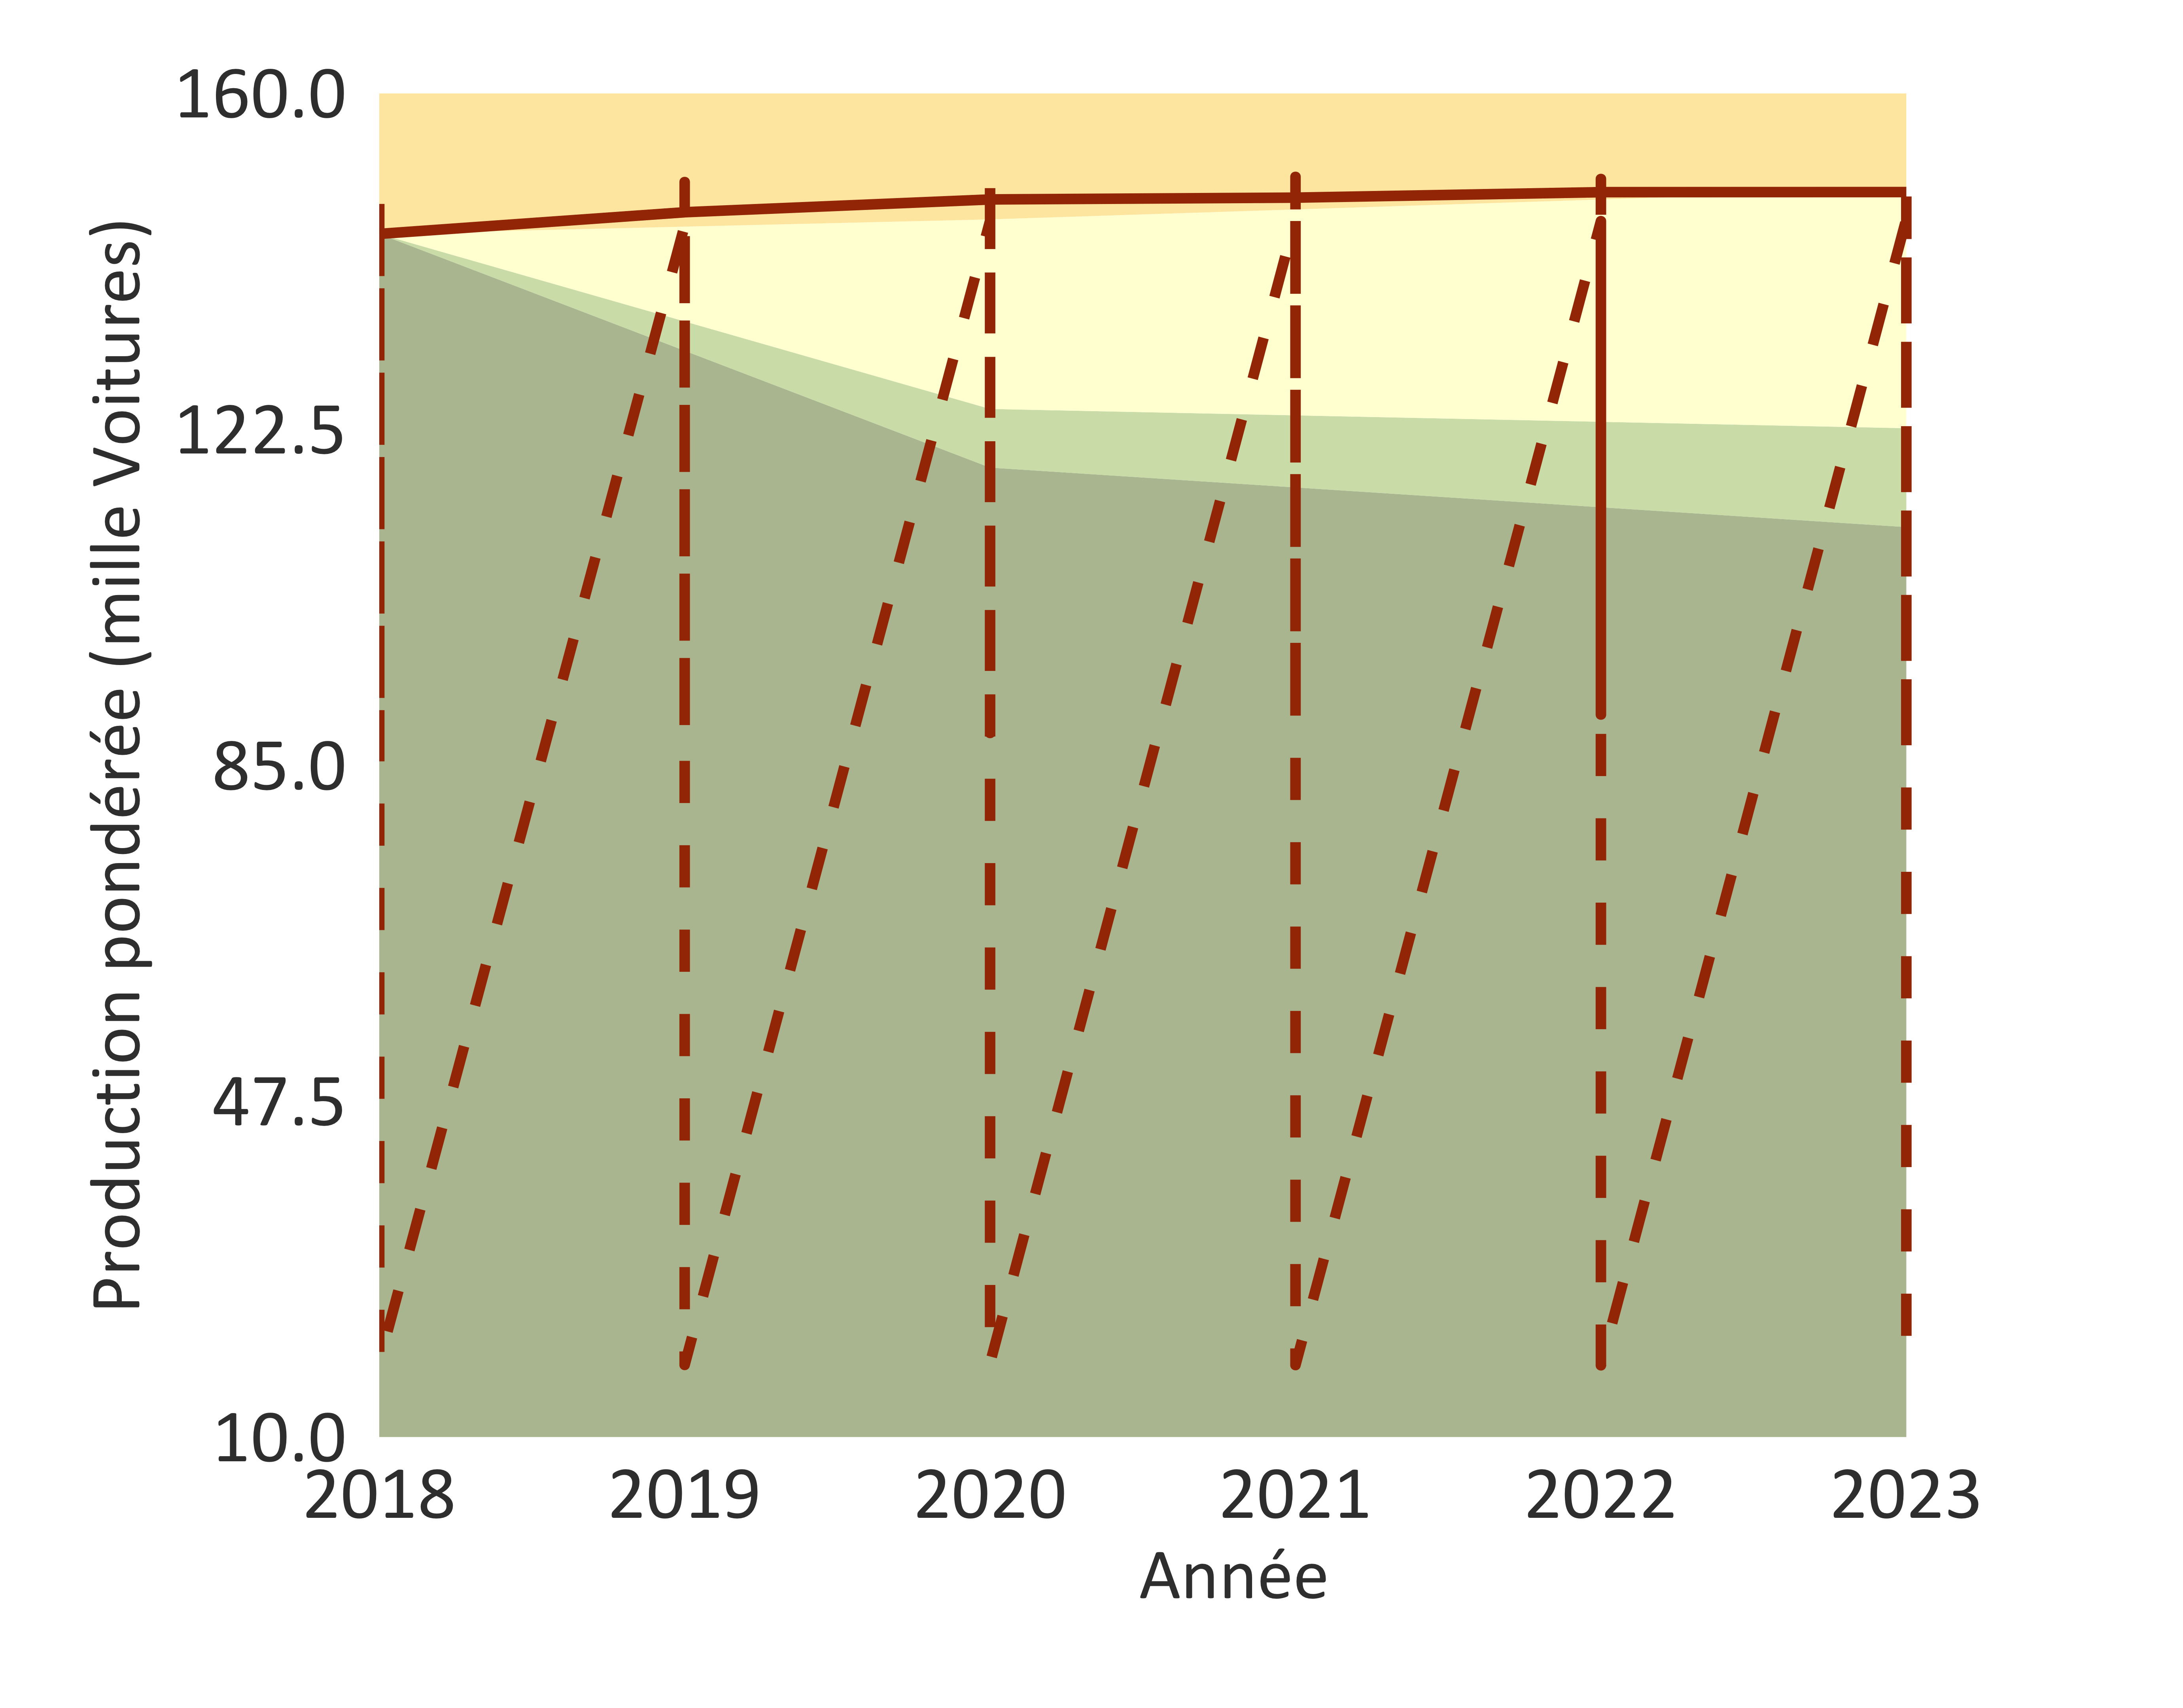
\includegraphics[trim = {0 0cm 0 0},width=1\linewidth]{ReportOutputs/Fig24}
		
	\end{minipage}	
	\hspace{.02\linewidth}
	\begin{minipage}[t]{.49\textwidth}
	\begin{center}
		\textbf{Trajectoire de la production des voitures électriques}
	\end{center}
		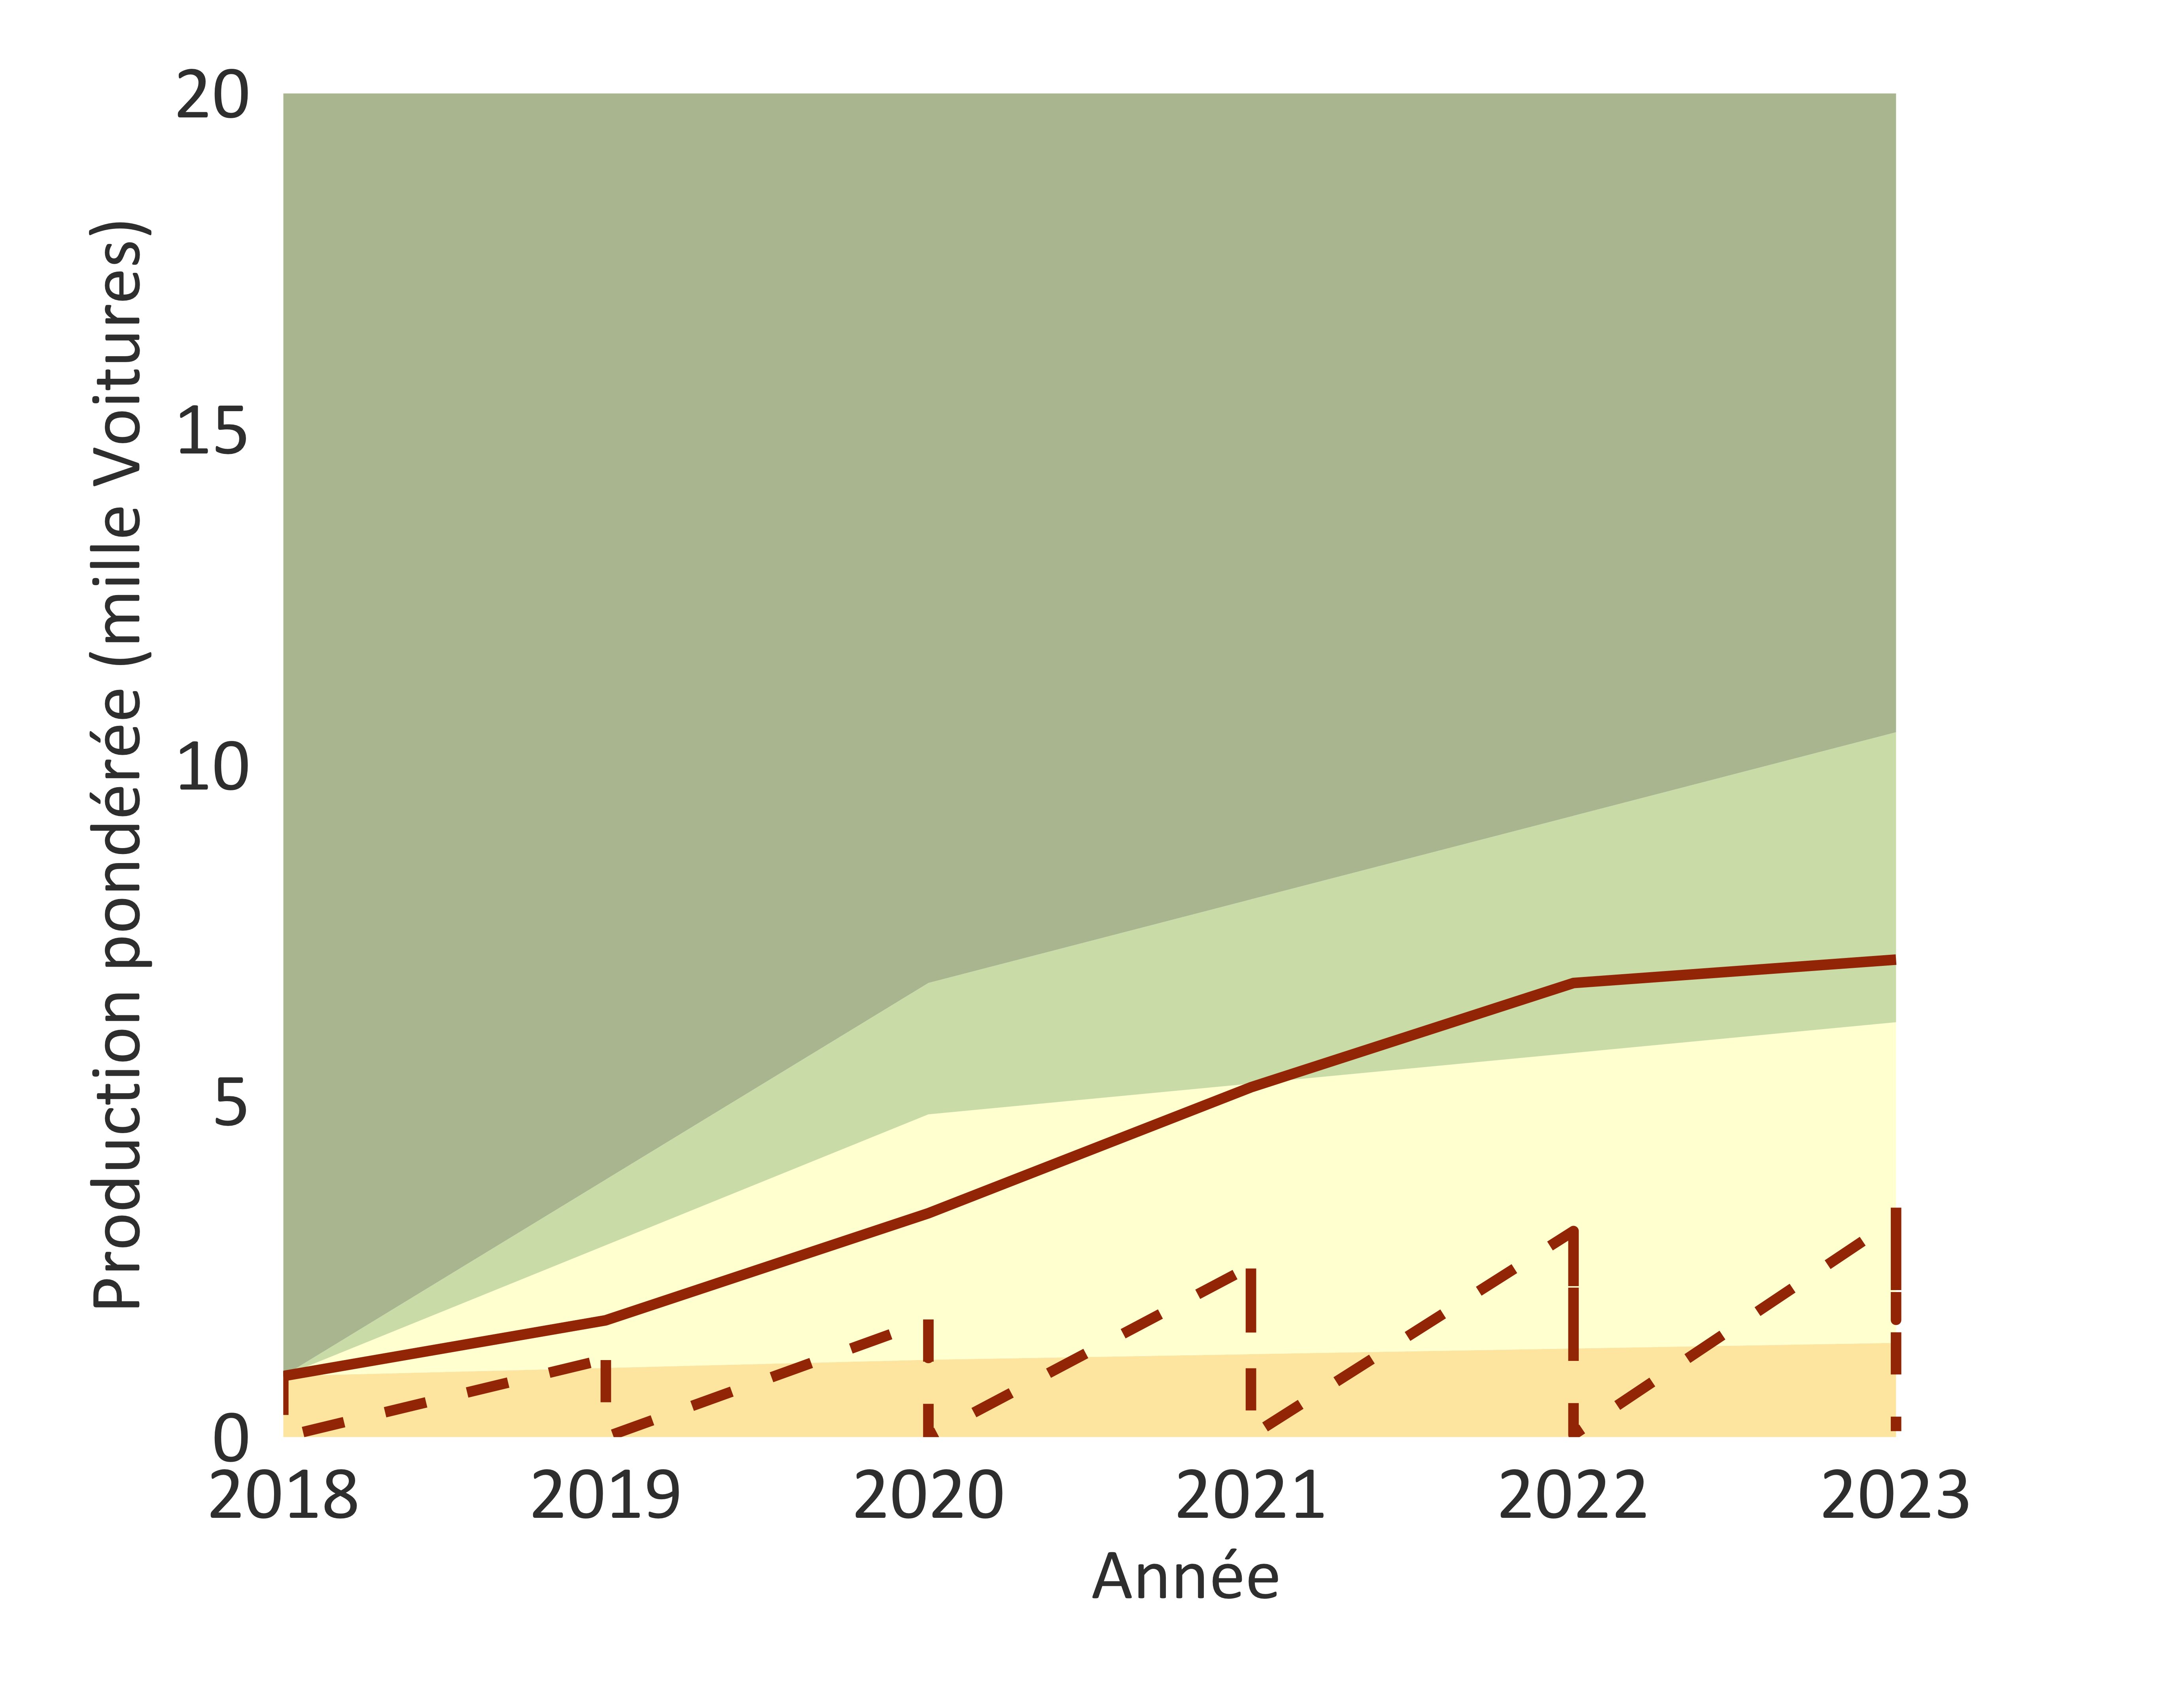
\includegraphics[trim = {0 0cm 0 0},width=1\linewidth]{ReportOutputs/Fig25}
		
	\end{minipage}	
	
	\begin{minipage}[t]{.49\textwidth}
	\begin{center}
		\textbf{Trajectoire de la production des voitures hybrides}
	\end{center}
		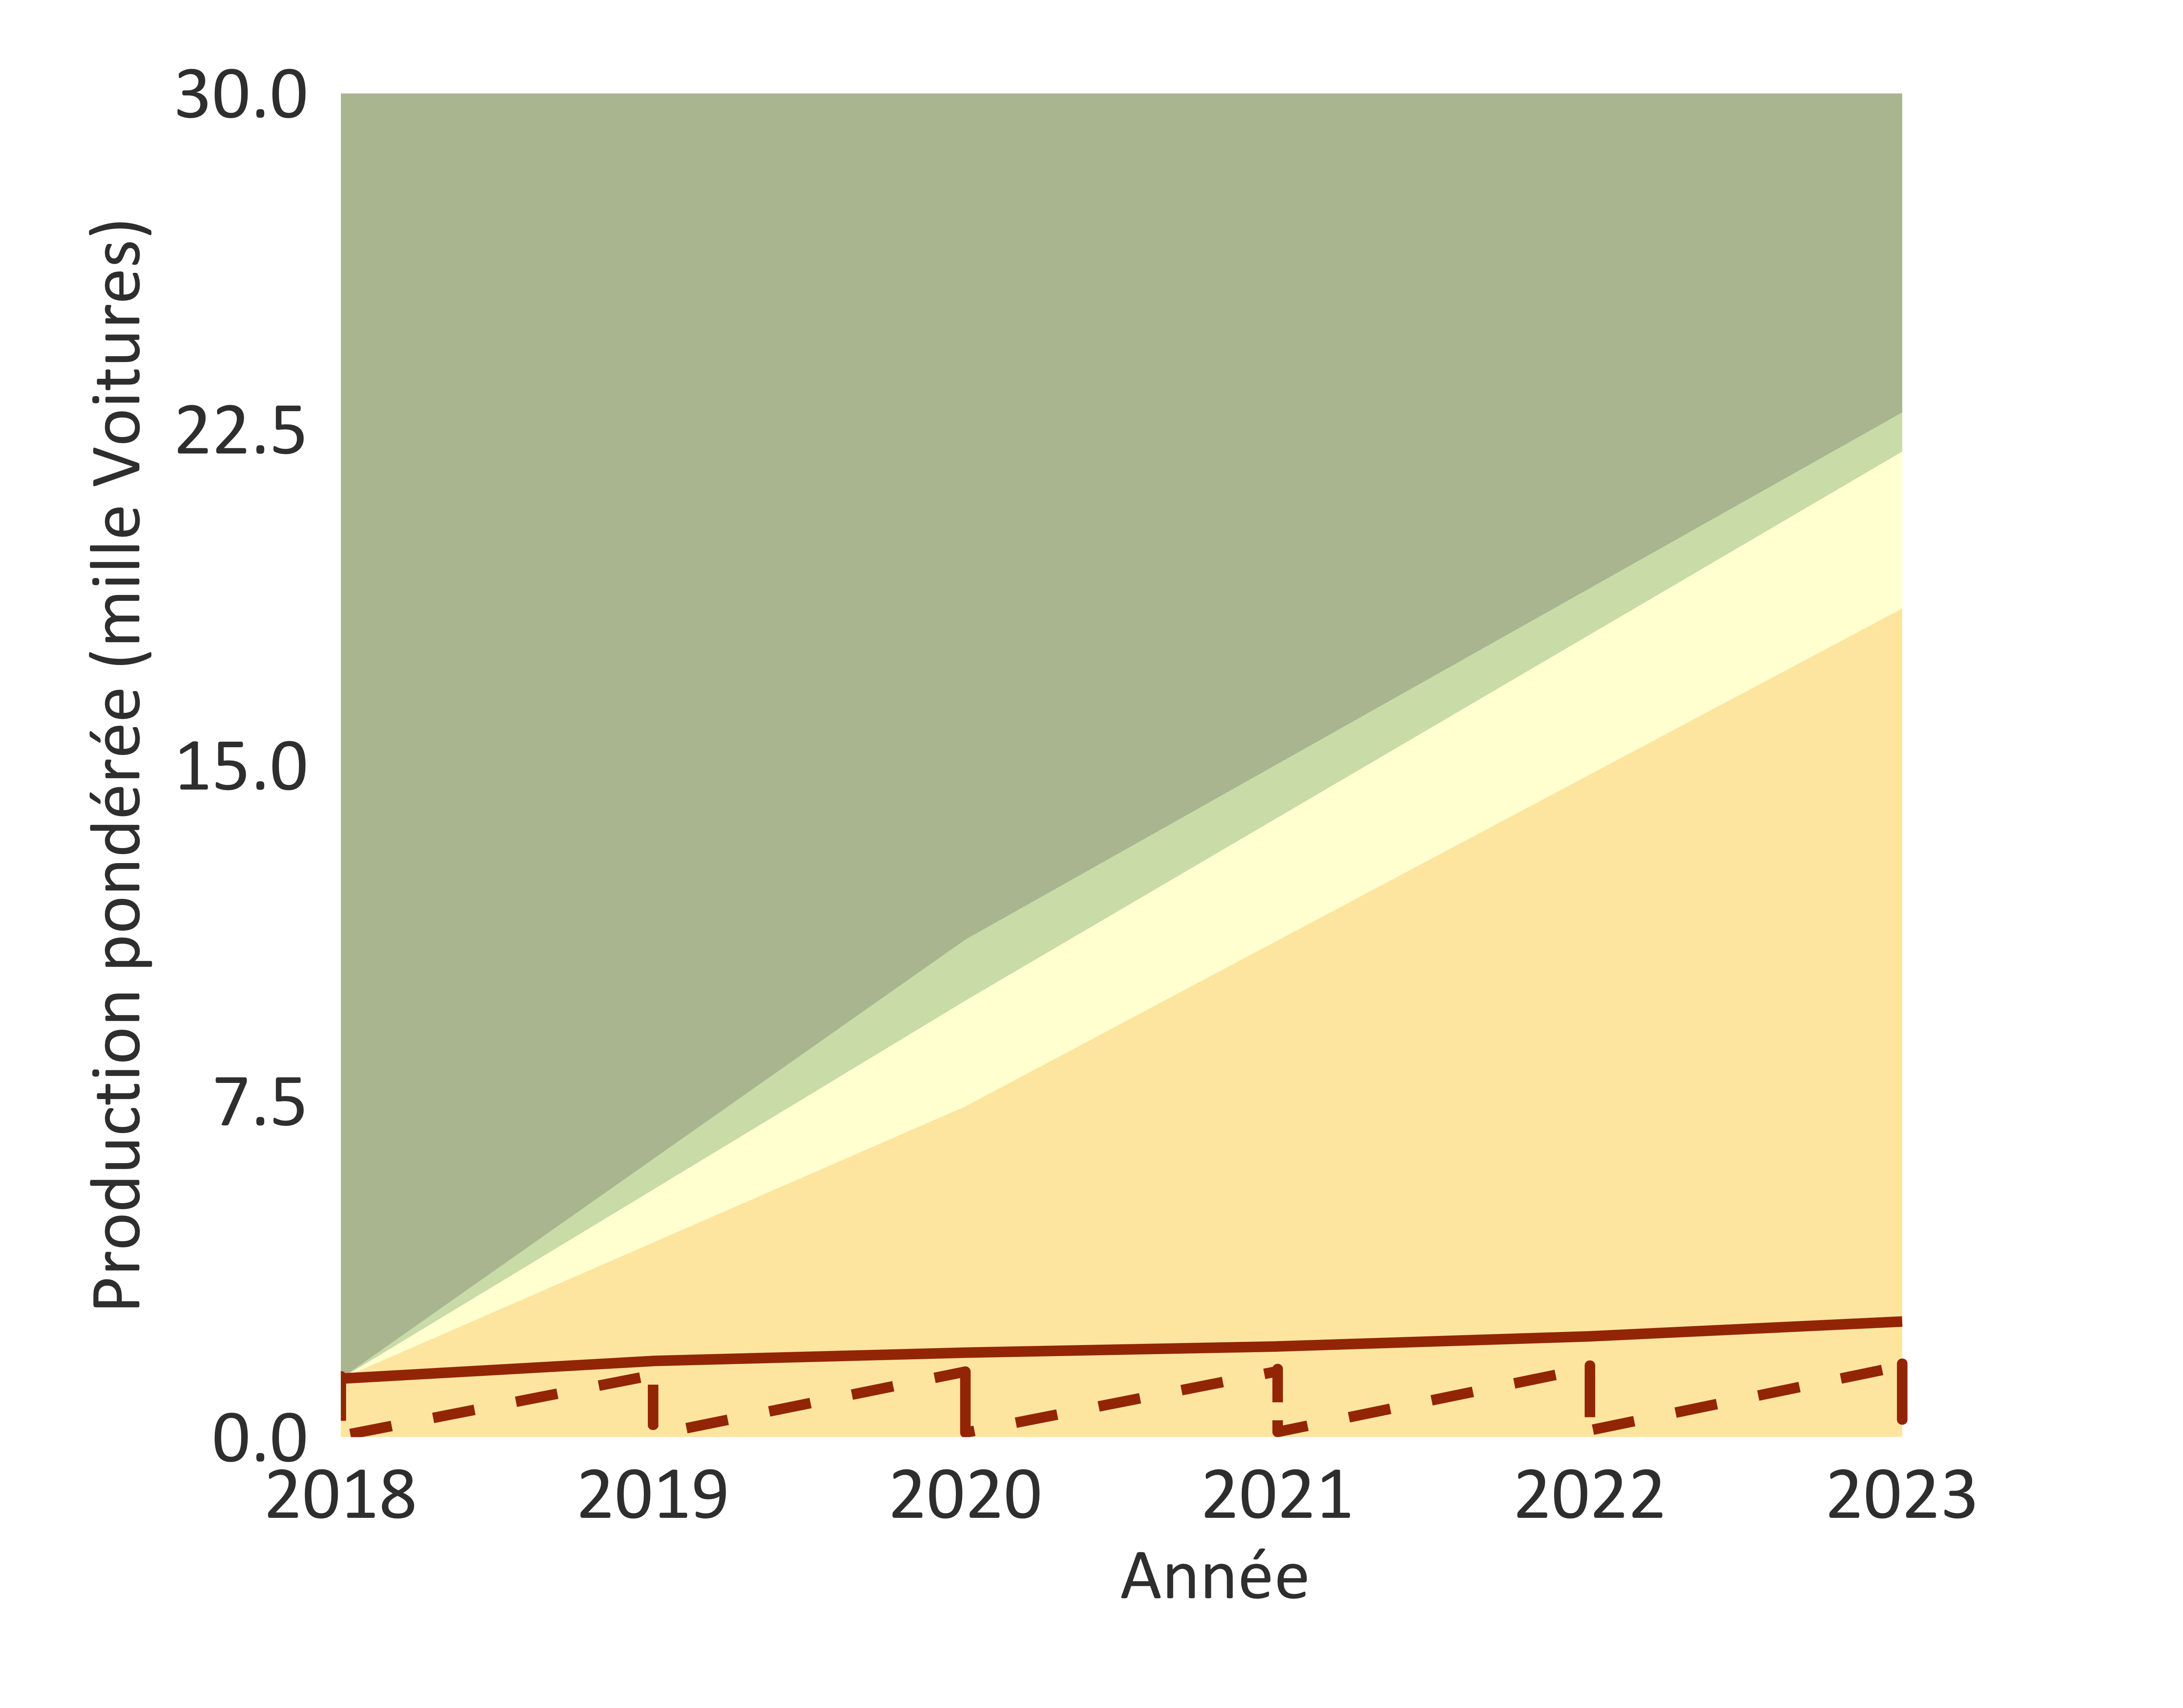
\includegraphics[trim = {0 0cm 0 0},width=1\linewidth]{ReportOutputs/Fig26}
		
	\end{minipage}		
	
	\vspace{-.1cm}
	\begin{center}
		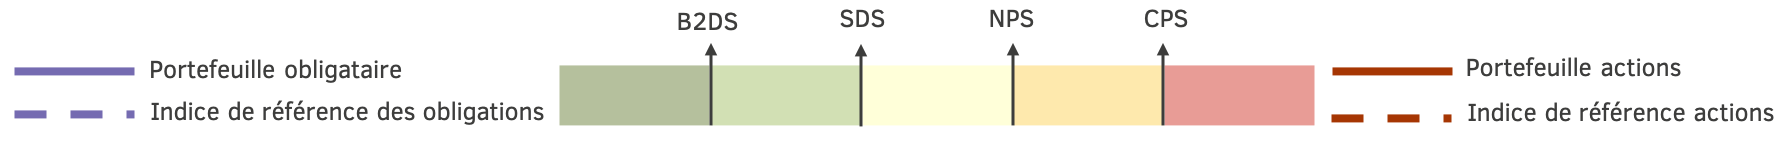
\includegraphics[trim = {0 0cm 0 0},width=1\linewidth]{ReportGraphics/246Legend_FR.png}
	\end{center}
	
	
	\PageFooterThird
	\newpage 
	%AutoSector_EQE
	%AutoSector_ALLE
	%OtherSectorsS
	\section*{} % OTHER SECTORS 
	\HeaderSingle{ANALYSE D’INTENSITE D’EMISSIONS}
	
	\begin{multicols}{2}
		Il existe un certain nombre de secteurs pour lesquels soit, il n'existe pas, à l'échelle du marché, de technologies alternatives à faible intensité carbone ou alors pour lesquels il est impossible d'obtenir des données sur les actifs et/ou les scénarios. Cela concerne les secteurs de l'acier, du ciment, et du transport maritime. Pour ces secteurs, une analyse de l'évolution requise de l'intensité d'émissions est effectuée.
		Pour ces secteurs, les efforts de décarbonisation consistent à augmenter l’efficacité énergétique lors des étapes de production et d'utilisation, ainsi que les investissements dans la R\&D au cours des 5 à 10 années suivantes, afin d'ammener à maturité commerciale, à moyen terme, des alternatives technologiques neutres en CO\textsubscript{2}. Par conséquent, les scénarios et les données sont relativement imprécis.

		Les graphiques présentés ci-dessous sont basés sur des estimations externes de l'intensité des émissions de CO\textsubscript{2}, provenants d'un modèle d'estimation des émissions accessible au public développé par 2Dii en collaboration avec la société de conseil Ernst\& Young. Pour le transport maritime, un modèle externe d'évaluation des émissions de CO\textsubscript{2}, qui a été mis au point par Rightship et Carbon War Room, a été utilisé. Une note de A indique que le navire est le meilleur de sa catégorie et une note de G, le pire de sa catégorie. Comme ce modèle est externe, et a recours a une approche « top down », il est associé à certaines incertitudes. Les résultats doivent donc être considérés comme des estimations, contrairement à l'analyse des scénarios des secteurs électriques, des combustibles fossiles et de l'automobile. Pour plus d'informations, se reporter à la section 6.
		
	\end{multicols}
	\vspace{0.3cm}
	\begin{multicols}{2}
		\begin{center}
		\textbf{Ciment}
		\end{center}
    	\begin{center}
		\textbf{Navigation}
		\end{center}
	\end{multicols}
	
	\setlength\multicolsep{0pt}
	\vspace{0cm}
	
	\begin{multicols}{2}
		
		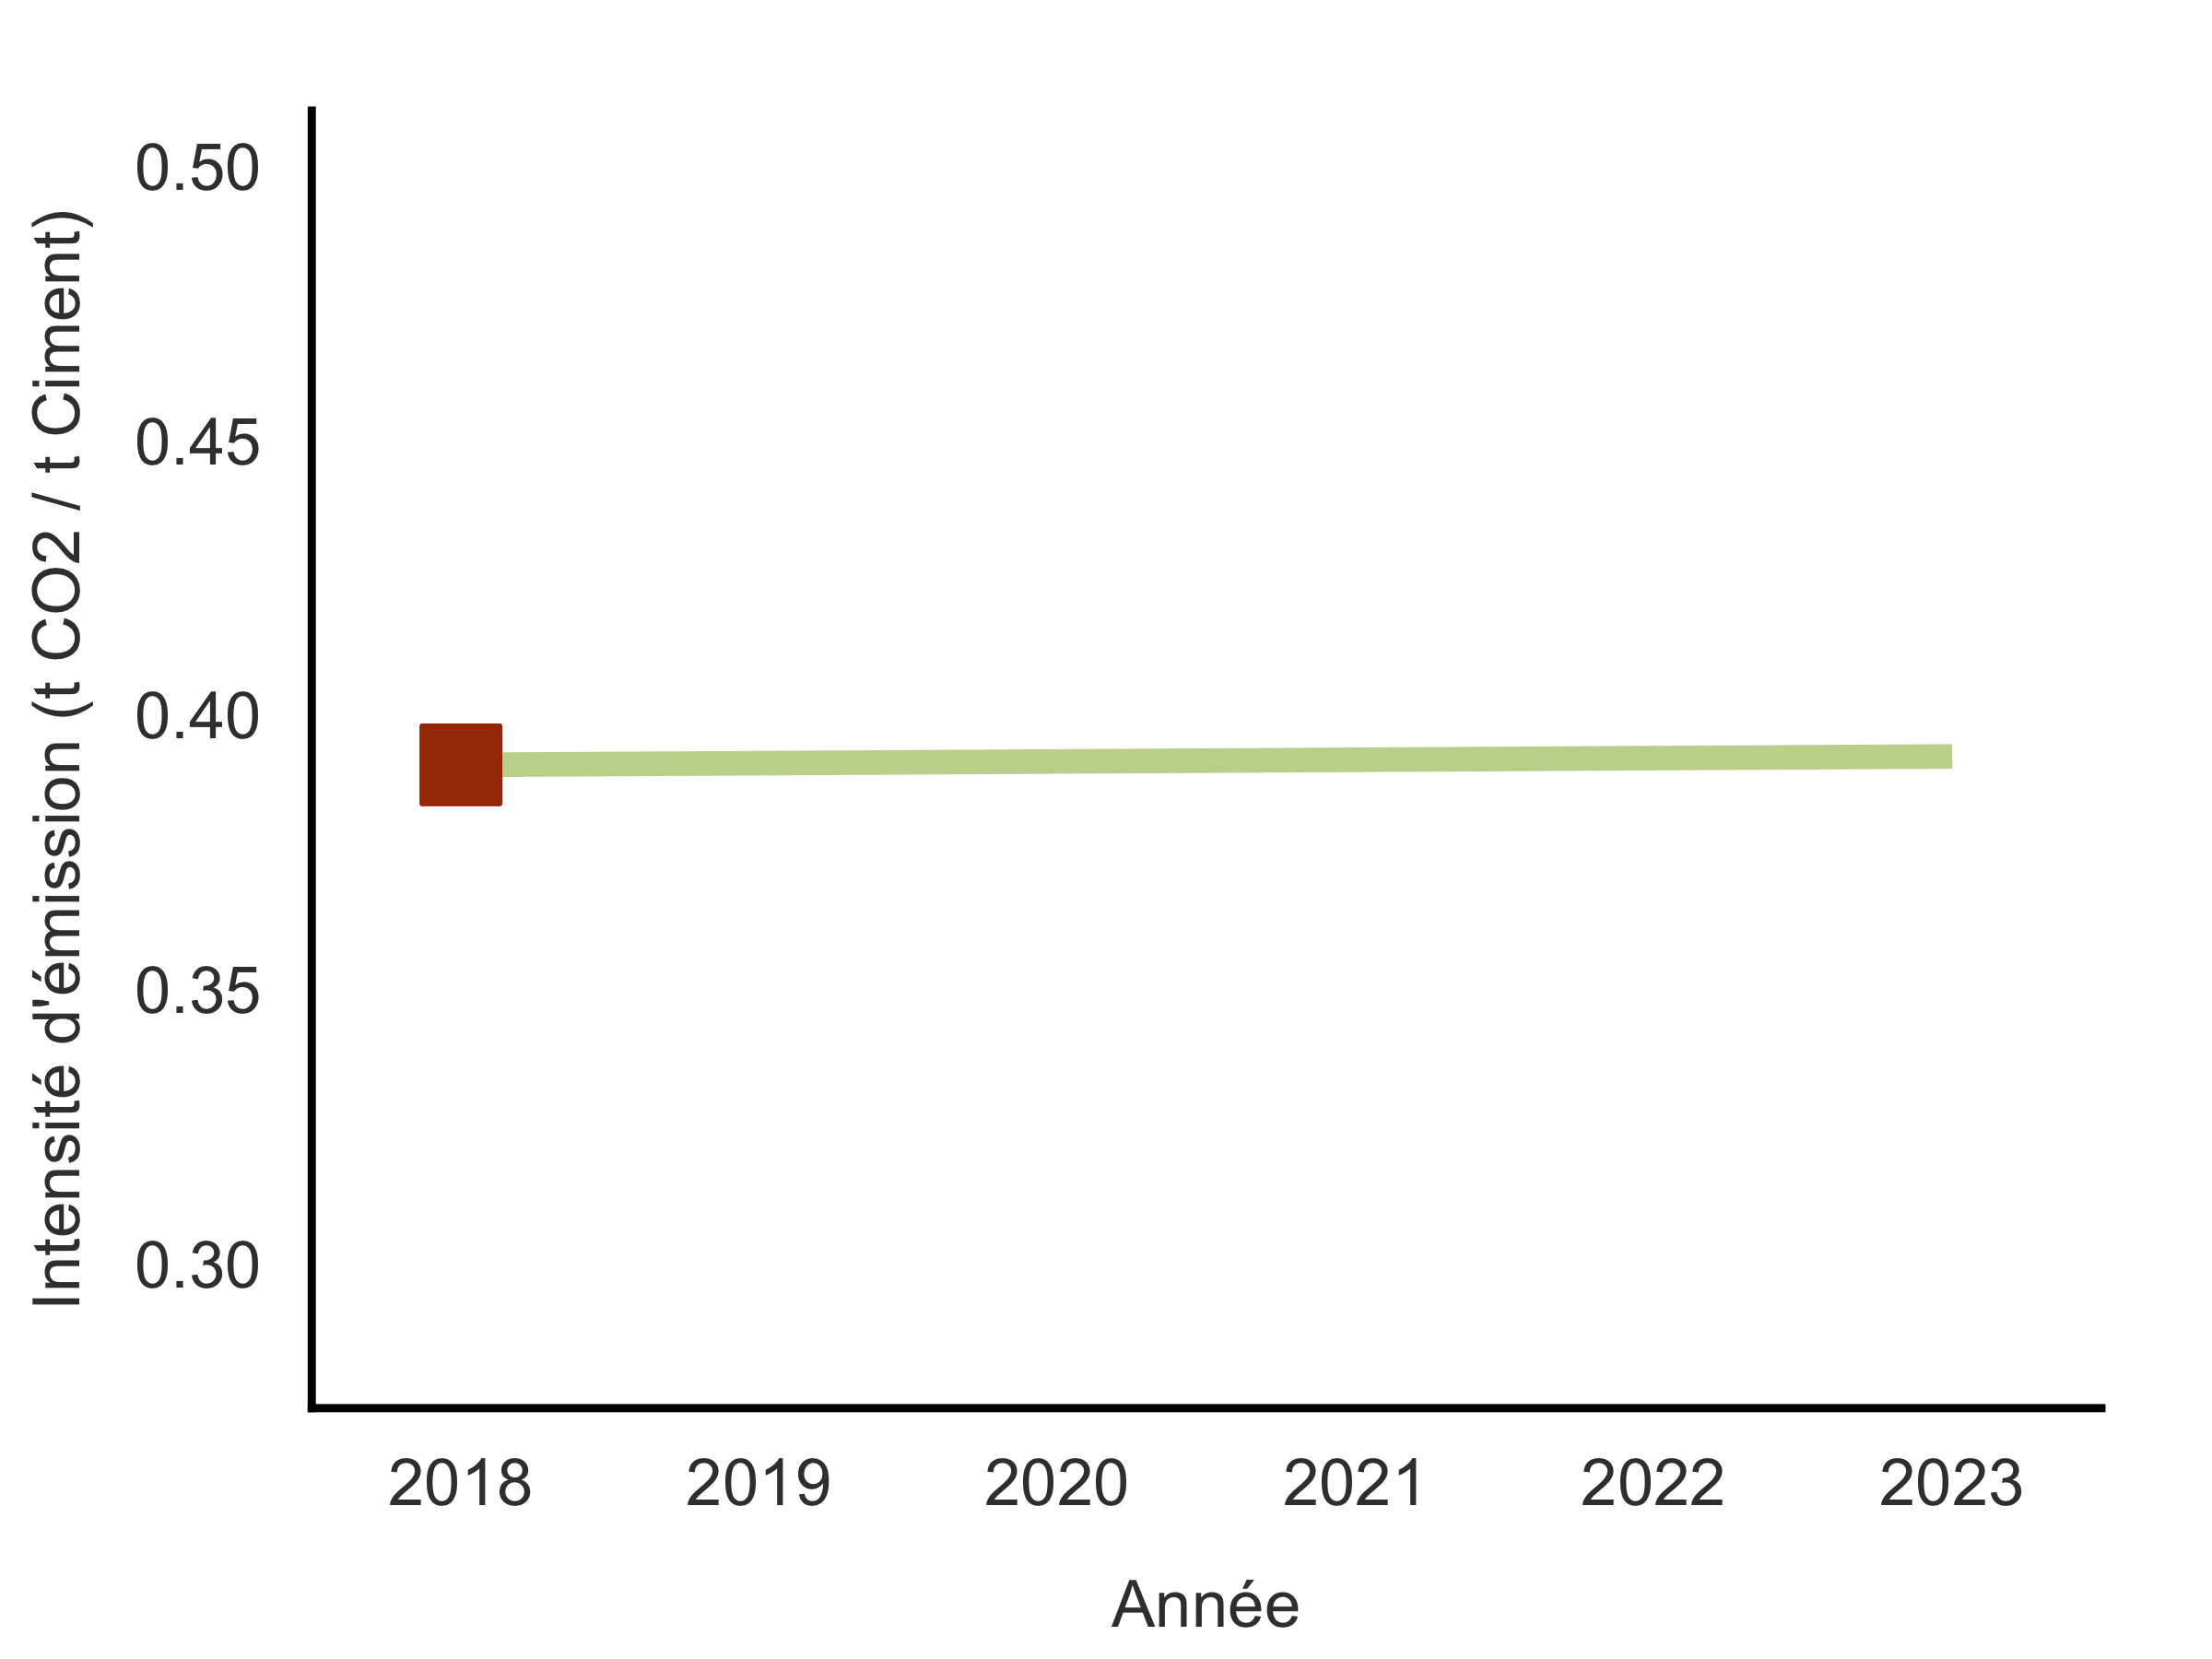
\includegraphics[width=.9\linewidth]{ReportOutputs/Fig30} \vfill\null \columnbreak
		
		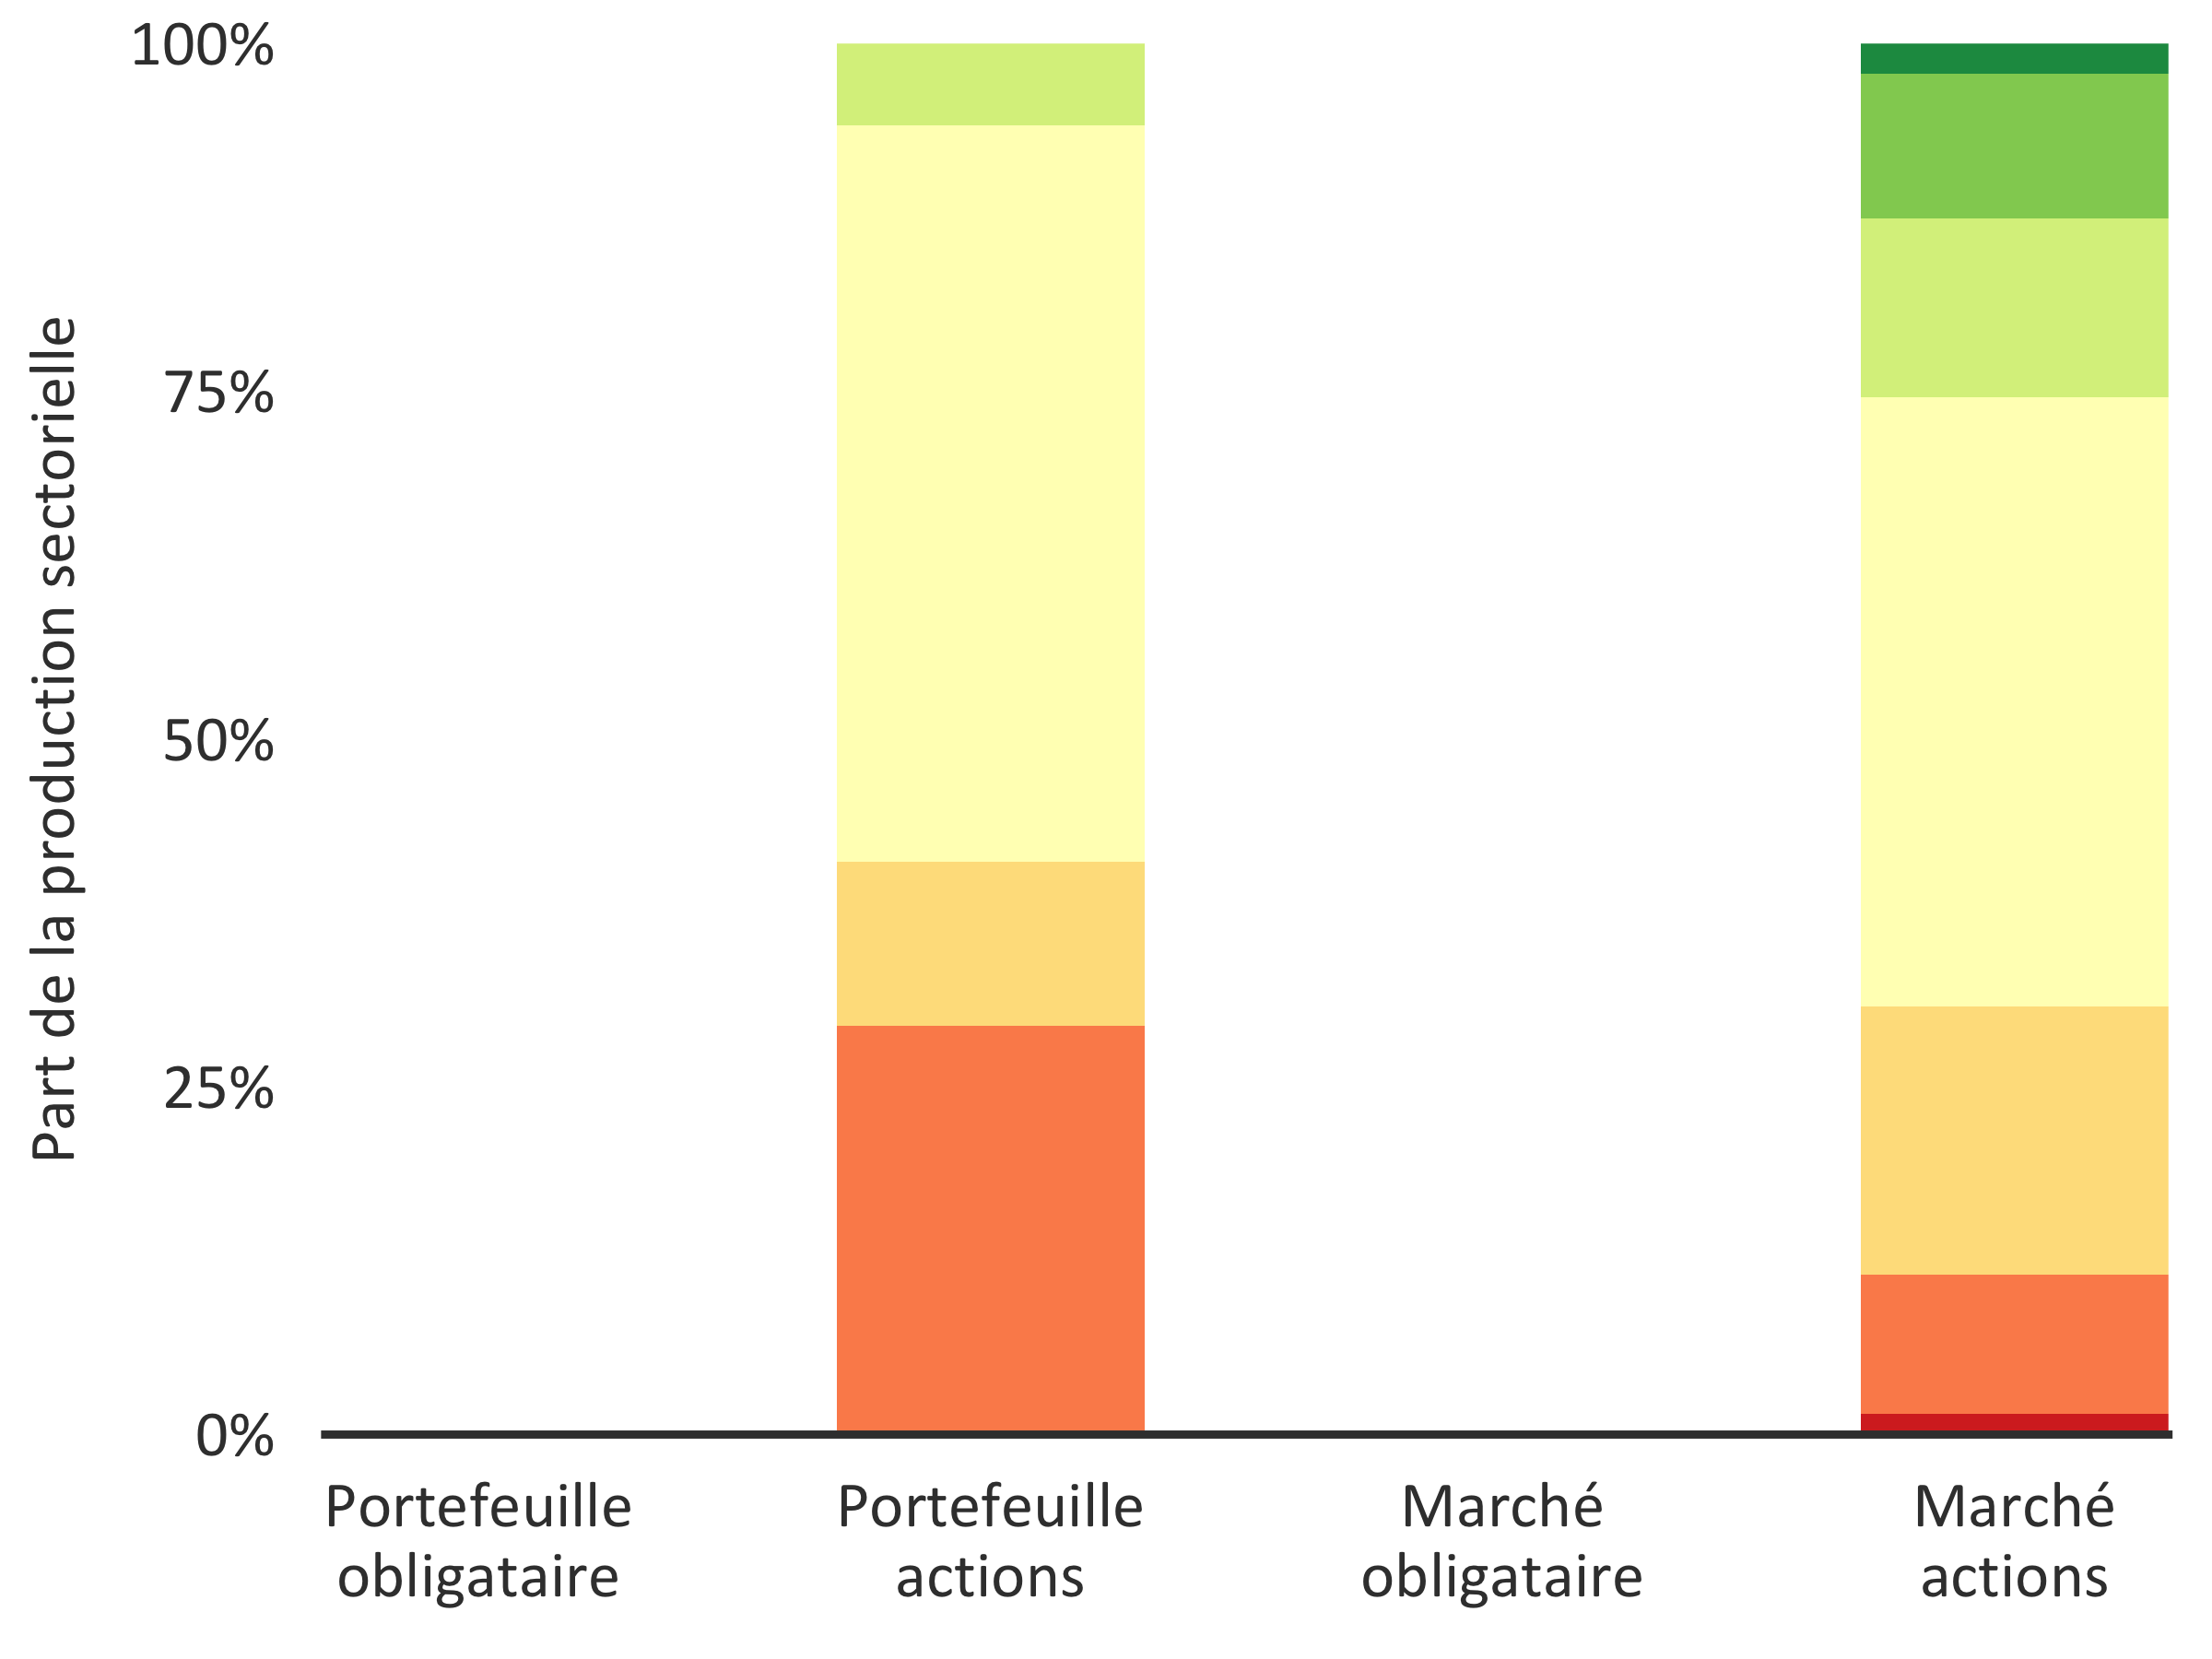
\includegraphics[width=.9\linewidth]{ReportOutputs/Fig33}
		\begin{center}
			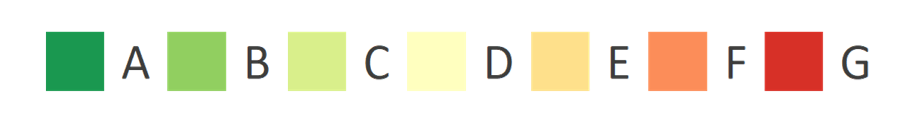
\includegraphics[width=0.6\linewidth]{ReportGraphics/ShippingLegend}
		\end{center}	
		
	\end{multicols}
	
	\begin{multicols}{2}
		\begin{center}
		\textbf{Acier}
		\end{center}
	    \begin{center}
	%%	\textbf{Navigation}
		\end{center}
	\end{multicols}
	
	\vspace{0.1cm}
	
	\begin{multicols}{2}
		
		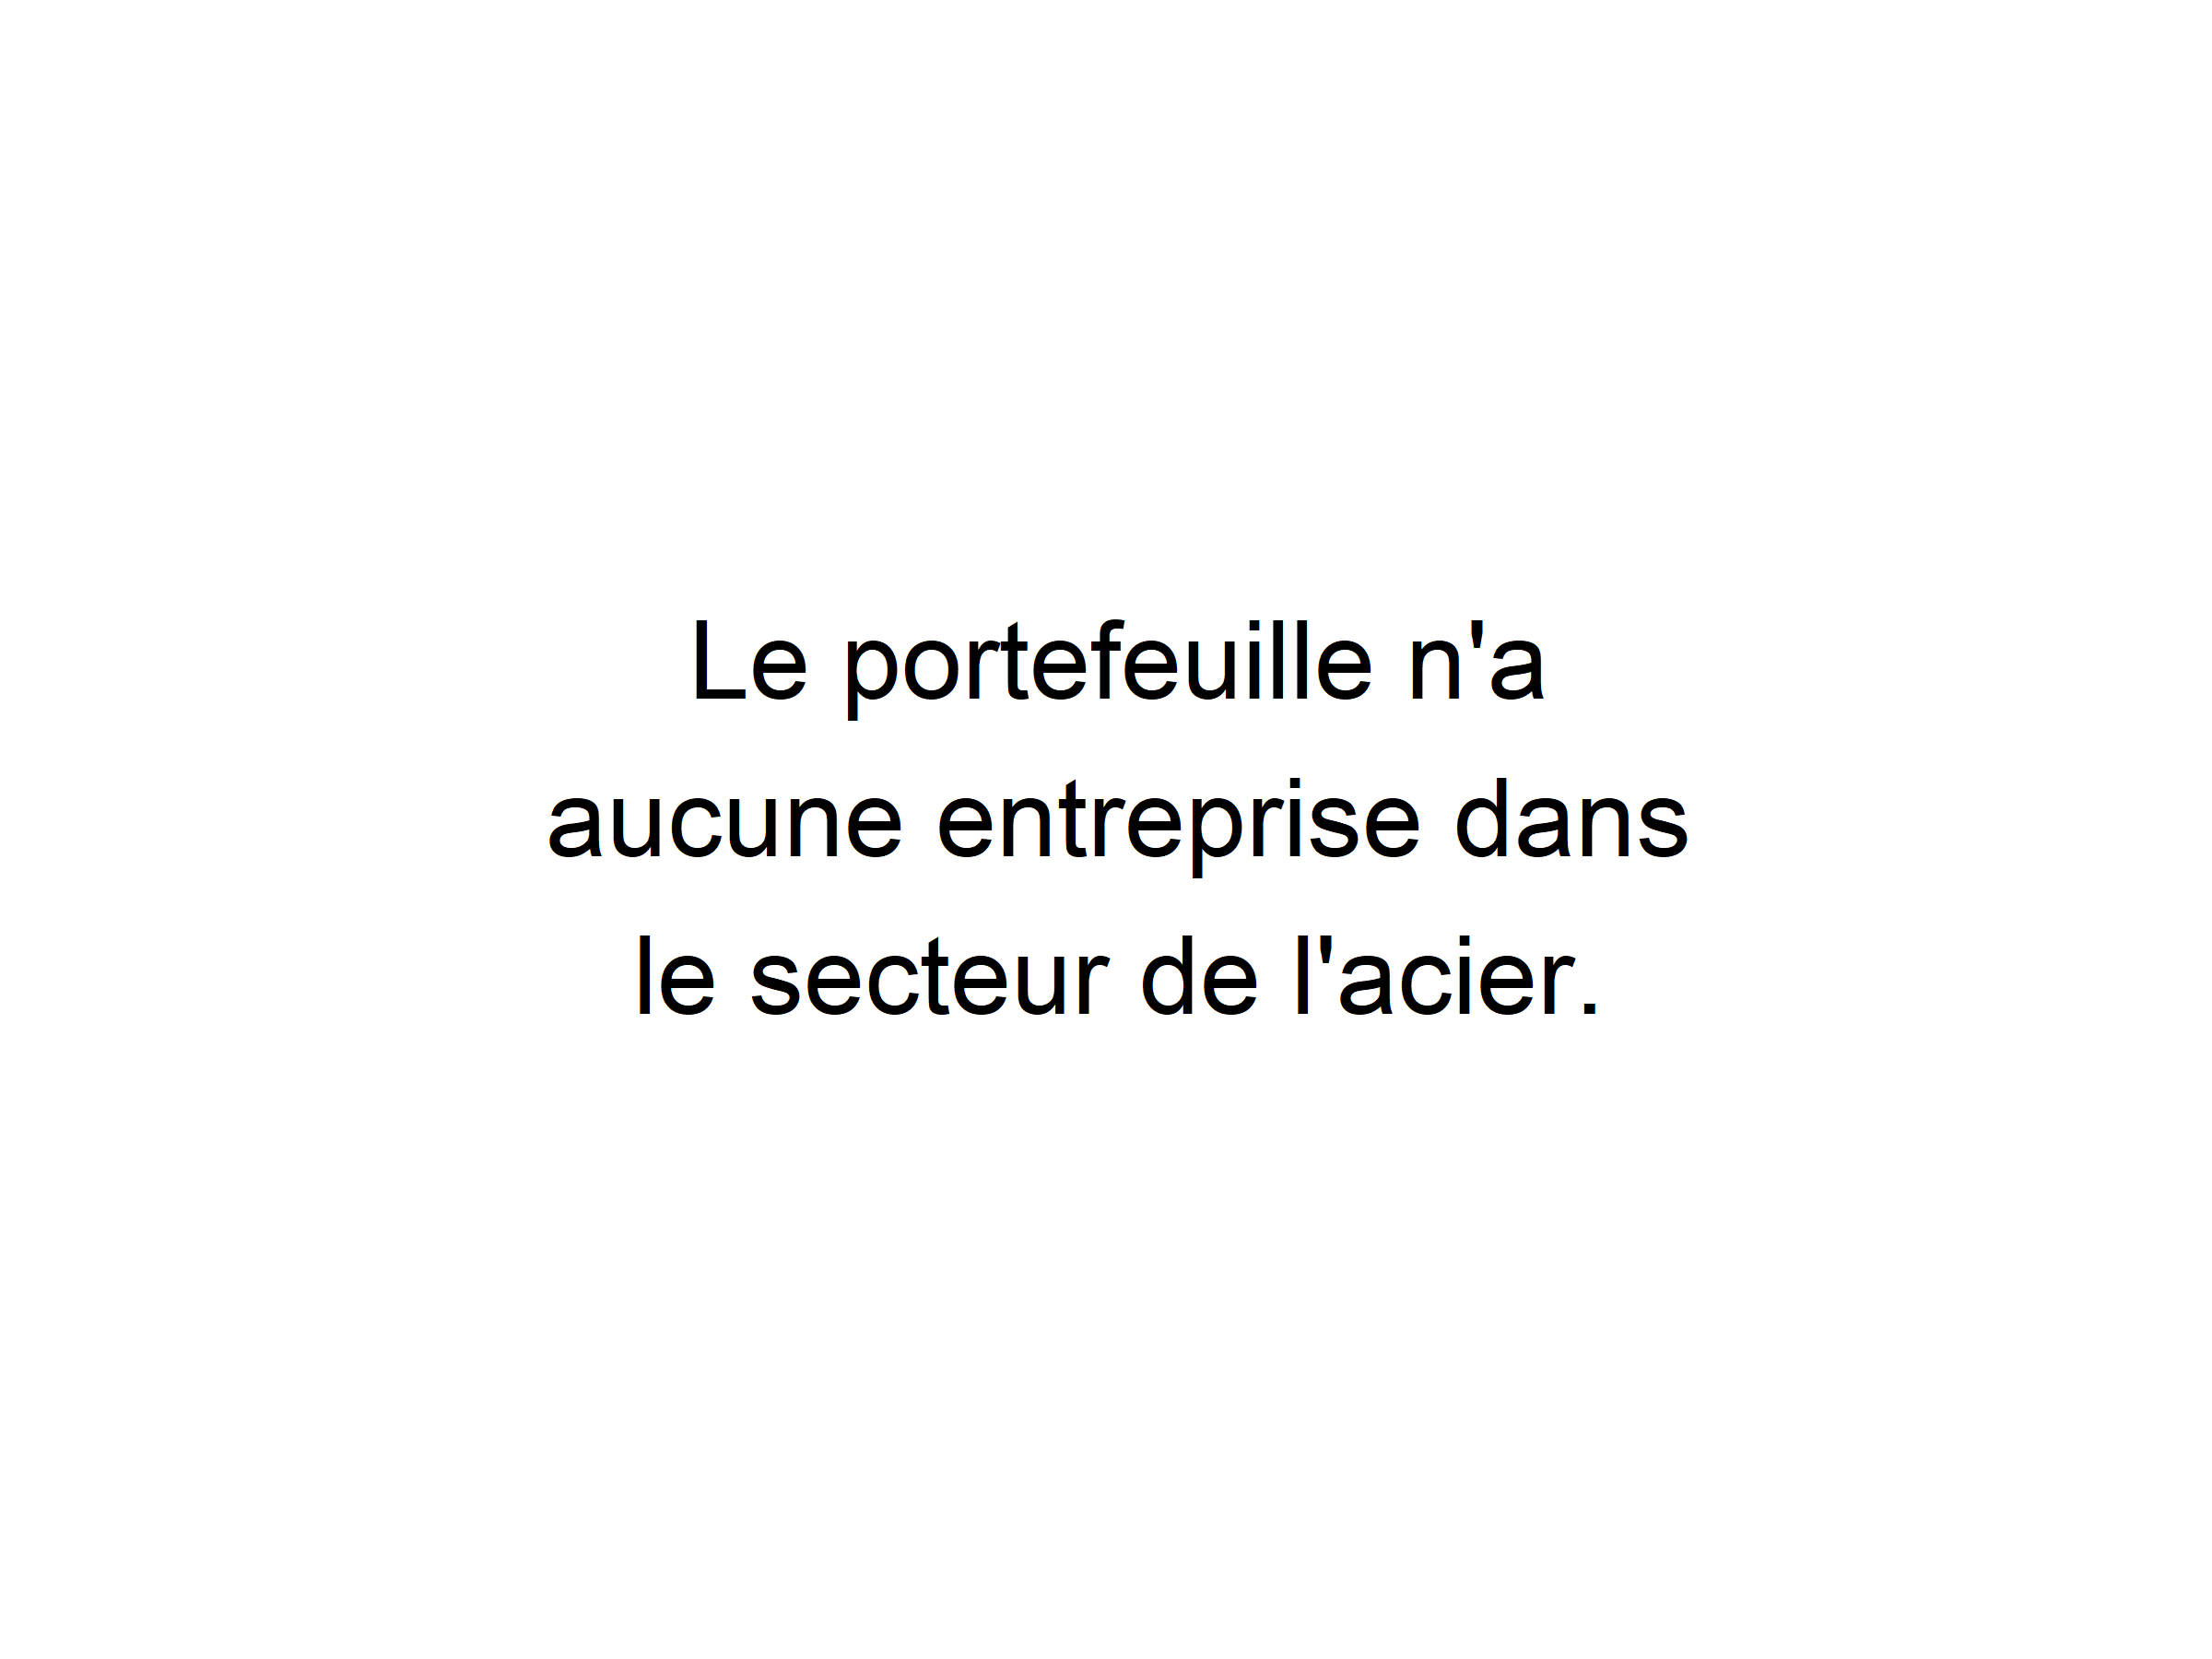
\includegraphics[trim = {0 0 0 0pt}, width=.9\linewidth]{ReportOutputs/Fig31}  \vfill\null \columnbreak
		
		%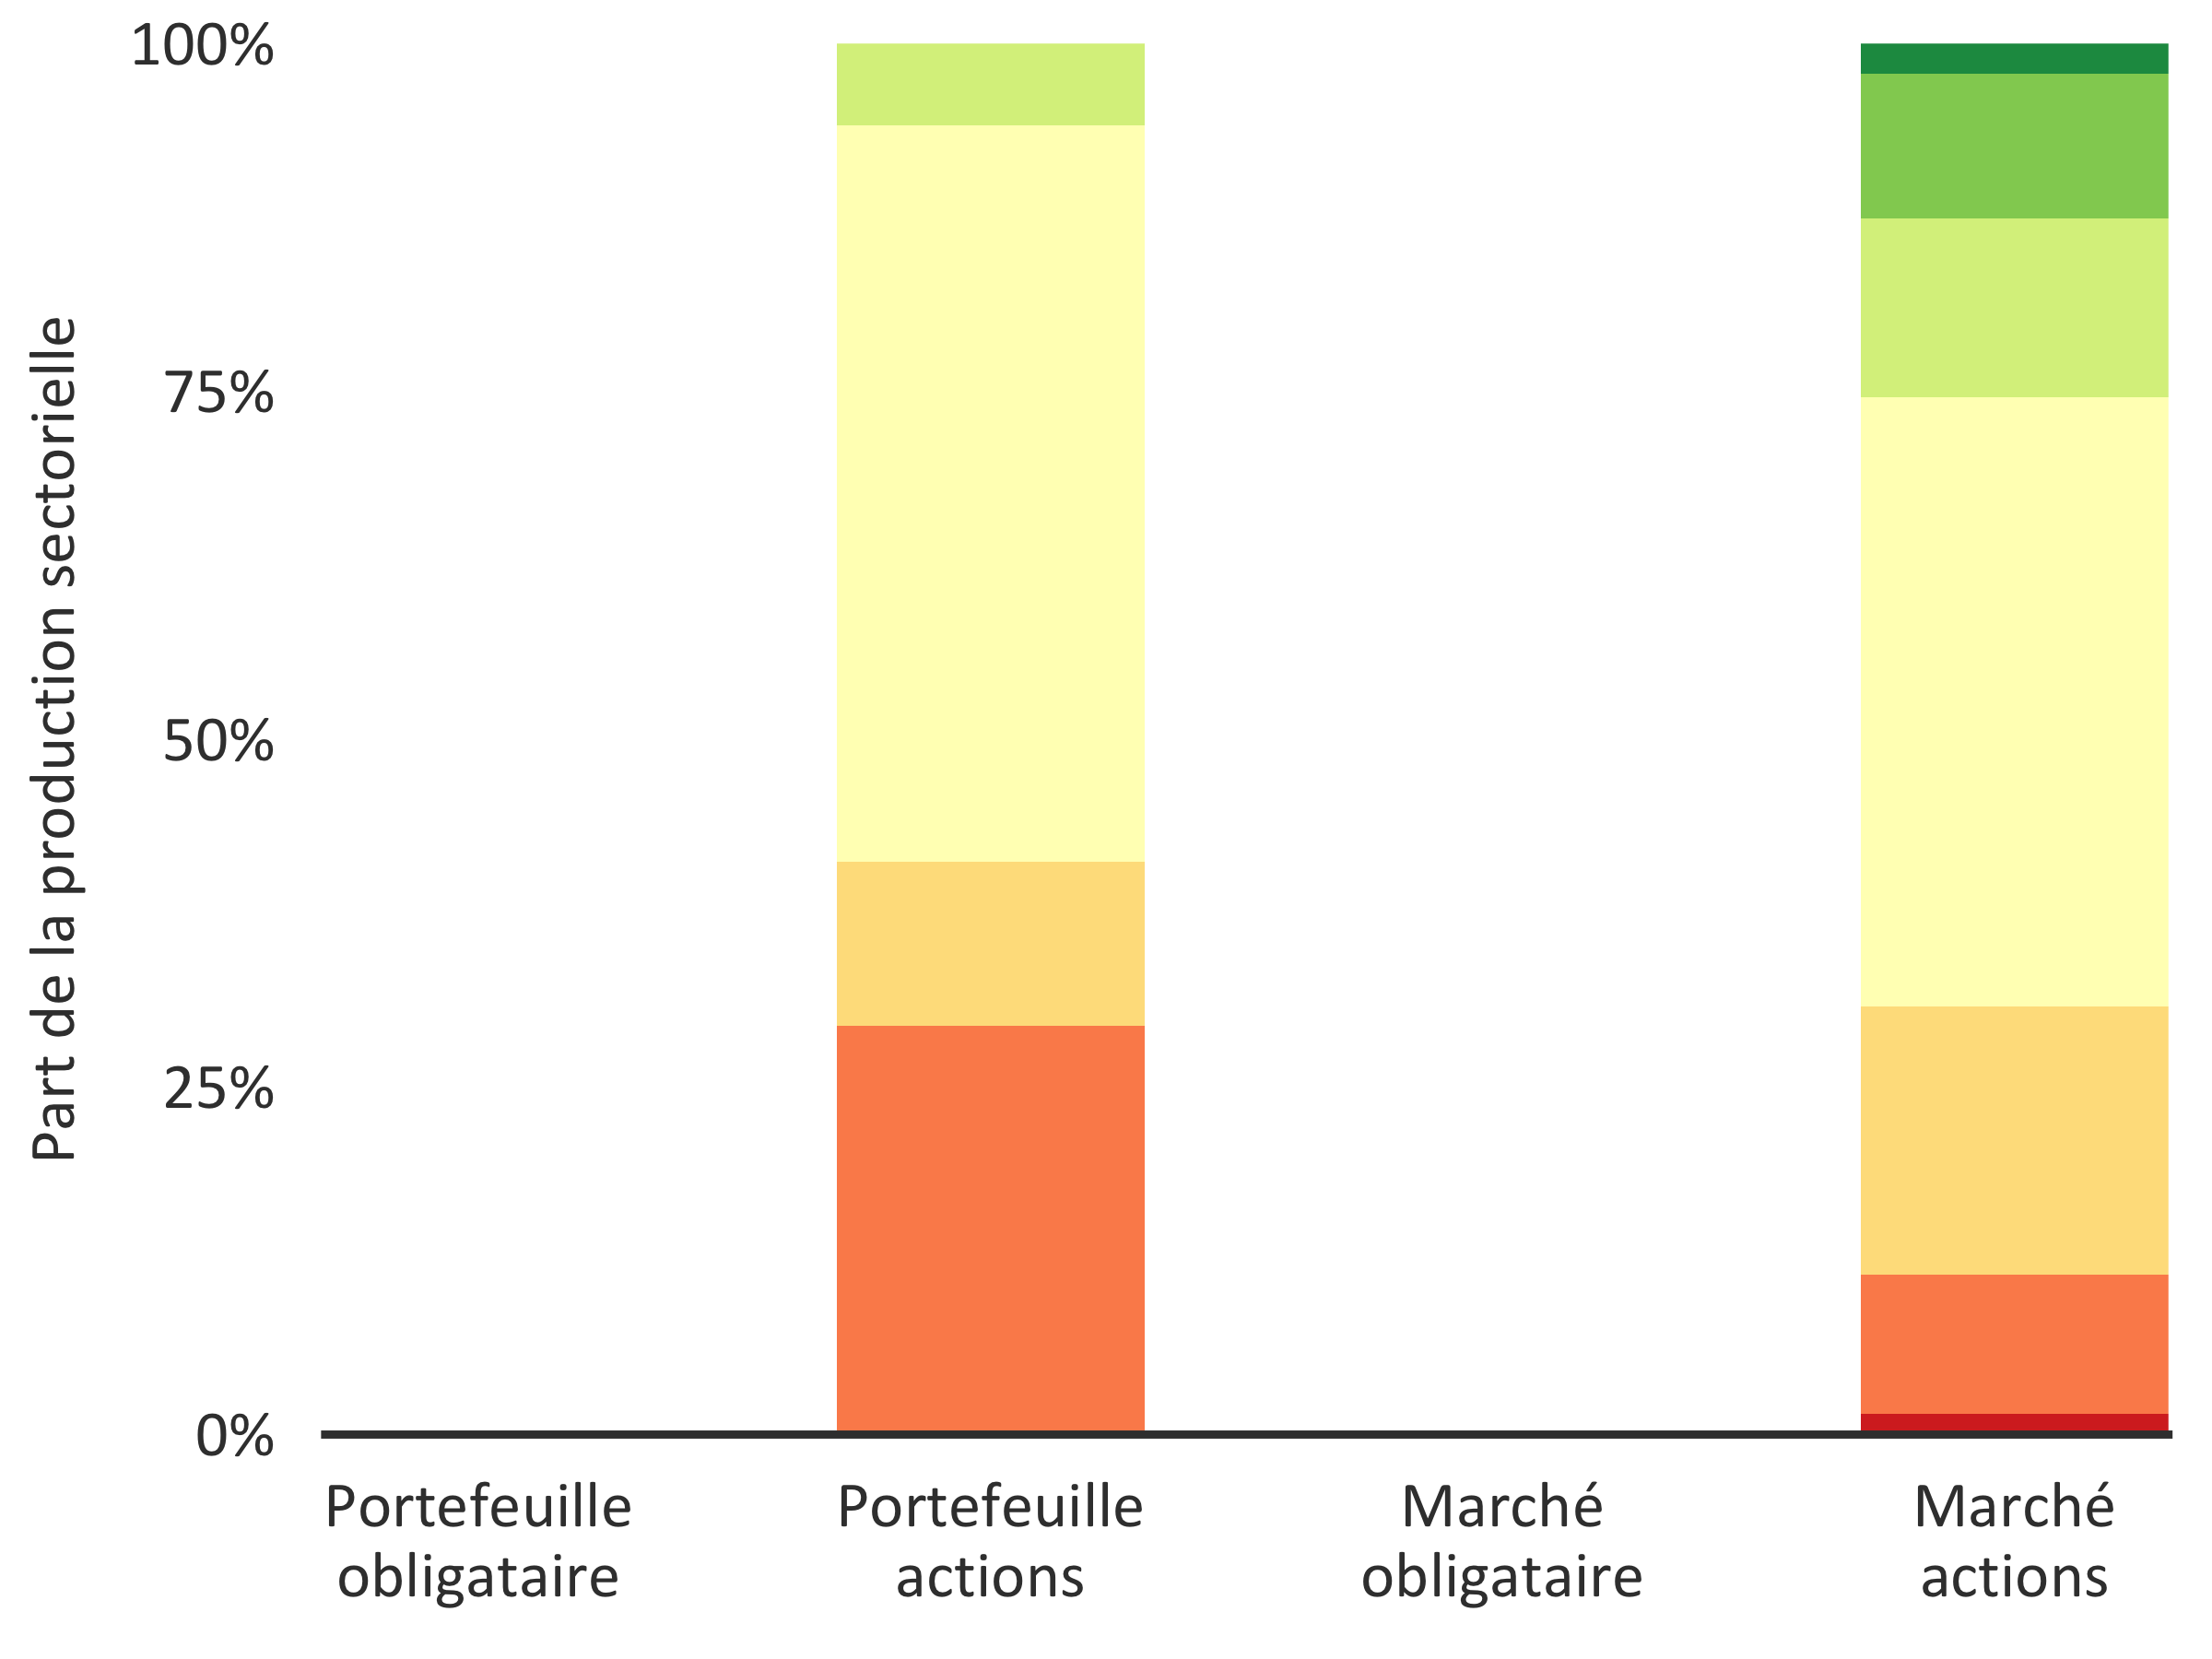
\includegraphics[width=0.9\linewidth]{ReportOutputs/Fig33}
		
	\end{multicols}
	
	\vspace{0cm}
	\setlength\multicolsep{0pt}
	
	\begin{multicols}{2}
		\vspace{0.2cm}
		 \begin{center}
	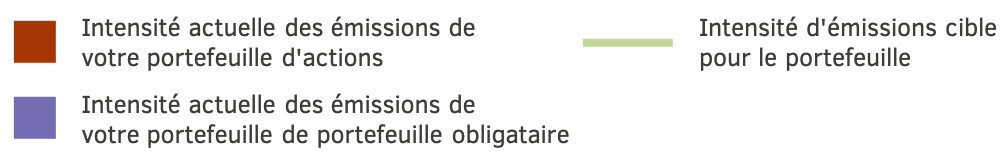
\includegraphics[width=1\linewidth]{ReportGraphics/EmissionsLegend_FR}
			\end{center}
	
		%NoShippingS
		%\begin{center}
		%	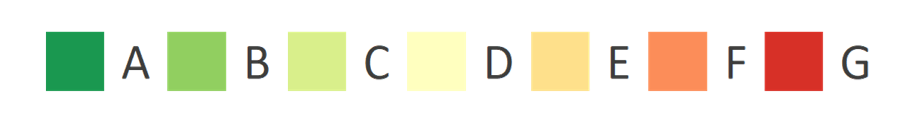
\includegraphics[width=0.6\linewidth]{ReportGraphics/ShippingLegend}
	%	\end{center}	
		%NoShippingE		
		
	\end{multicols}
  \vspace{0.3cm}
	\begin{center}
	\textit{\small Source: 2Dii basé sur EY 2016, PlantFacts, Rightship, Carbon War Room, IEA 2017 and SDA 2015}
	\end{center}
	\setlength\multicolsep{12pt}
	
	\PageFooterThird 
	\newpage 
	% OtherSectorsE
	\section*{} % 4th SECTION 
	\SectionHeadingDouble{SECCION 4:}{EXPOSITION ESTIMEE DU PORTEFEUILLE }{AU ScenarioValue EN Startyear+5}
	
	\newpage
	\section*{} % FUTURE TECHNOLOGY SHARE
	\HeaderSingle{FUTURE MIX TECHNOLOGIQUE ESTIME}
	
	\begin{multicols}{2}
		\textbf{Le graphique ci-dessous montre l'exposition estimée en Startyear+5 aux technologies à forte ou faible intensité carbone pour les secteurs des combustibles fossiles, électrique et automobile des énergies fossiles, de l'électricité et de automobile, tant dans le portefeuille d'obligations.}
		
	Les résultats sont issus du point de départ de l'exposition (section 2) et de l'évolution de l'exposition sur les 5 prochaines années (section 3) sur la base des plans d'investissement et de production actuels révélés pour toutes les technologies. Les résultats montrent l'exposition relative des portefeuilles à travers les classes d'actifs et les technologies/sources énergétiques. Les résultats sont comparés à un mix technologique aligné du marché dans le cadre d'une transition ScenarioName en Startyear+5. Pour les secteurs de l'électricité et de l'automobile, ces valeurs informent la métrique d'alignement.
	 
	L'analyse ne comprend pas d'hypothèses concernant les changements dans la composition du portefeuille. Elle se limite à l'analyse de la façon dont l'exposition du portefeuille aux technologies à forte et faible intensité carbone est appelée à changer au fil du temps en fonction de l'évolution de l'exposition des entreprises, indépendamment des changements de composition du portefeuille. Les résultats aident à contextualiser la part de l'exposition sectorielle en Startyear+5 exposée aux risques de transition en termes de la part des activités qui peuvent être classées à forte ou faible teneur en carbone. Étant donné la nature marginale des activités renouvelables dans les sociétés pétrolières et gazières, cette question n'a pas été prise en compte dans l'analyse, bien qu'elle puisse représenter une part croissante au fil du temps. Dans le secteur des combustibles fossiles, la production en unités physiques réelles, comme les barils, m\textsuperscript{3} ou tonnes, est convertie en GJ pour permettre la comparaison.
	\end{multicols}
	%CBSpecificS
	\vspace{-0.4cm}
	\textbf{Obligations d'entreprises} 
	\vspace{-0.35cm}
	\begin{center}
		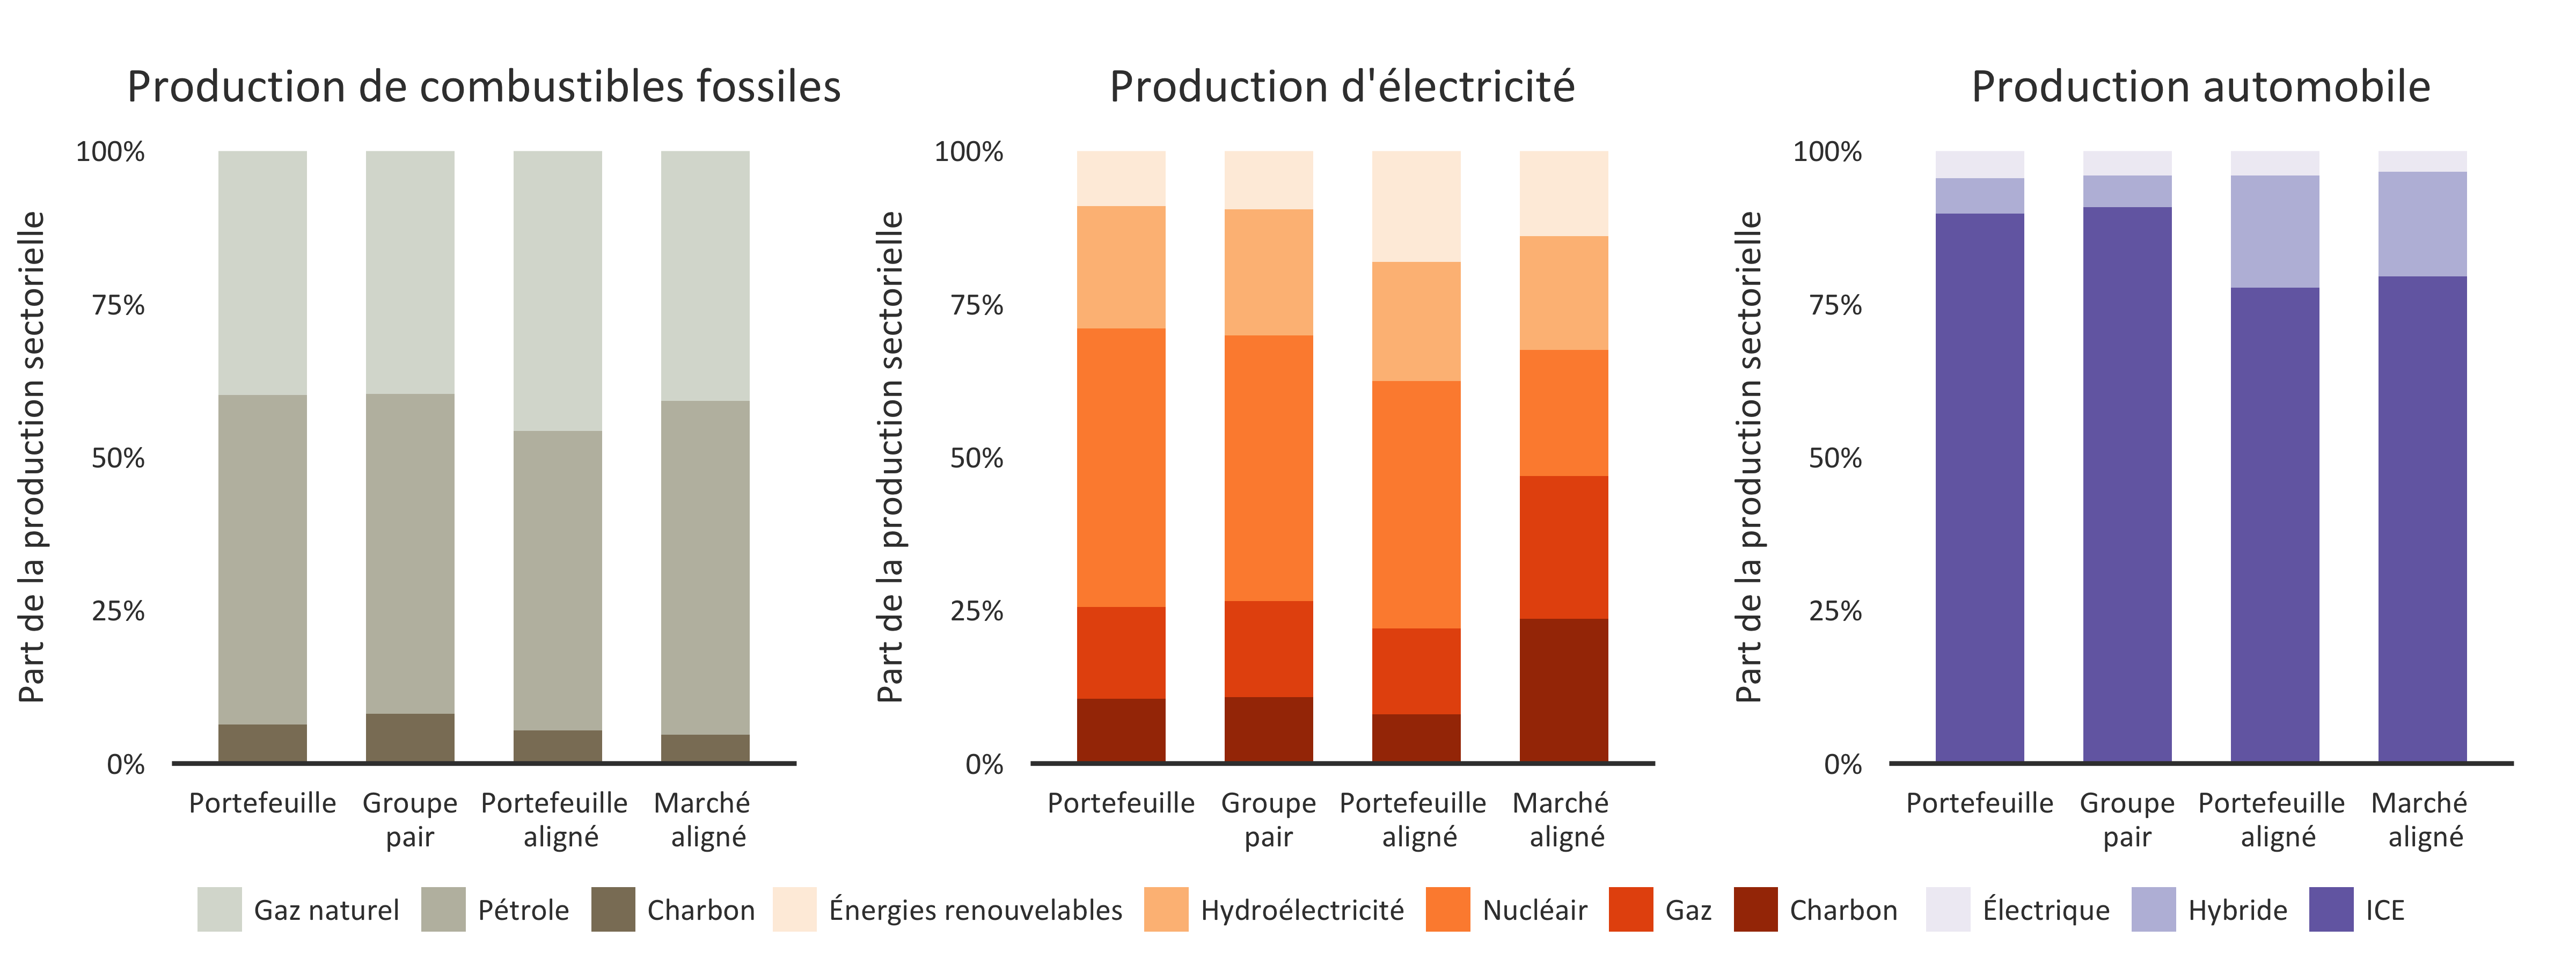
\includegraphics[trim = {0 0cm 0 0cm},width=1\linewidth]{ReportOutputs/Fig05}
	\end{center}
	%CBSpecificE	
	%EQSpecificS
	\vspace{-0.3cm}
	\textbf{Actions}
	\vspace{-0.35cm}
	\begin{center}
		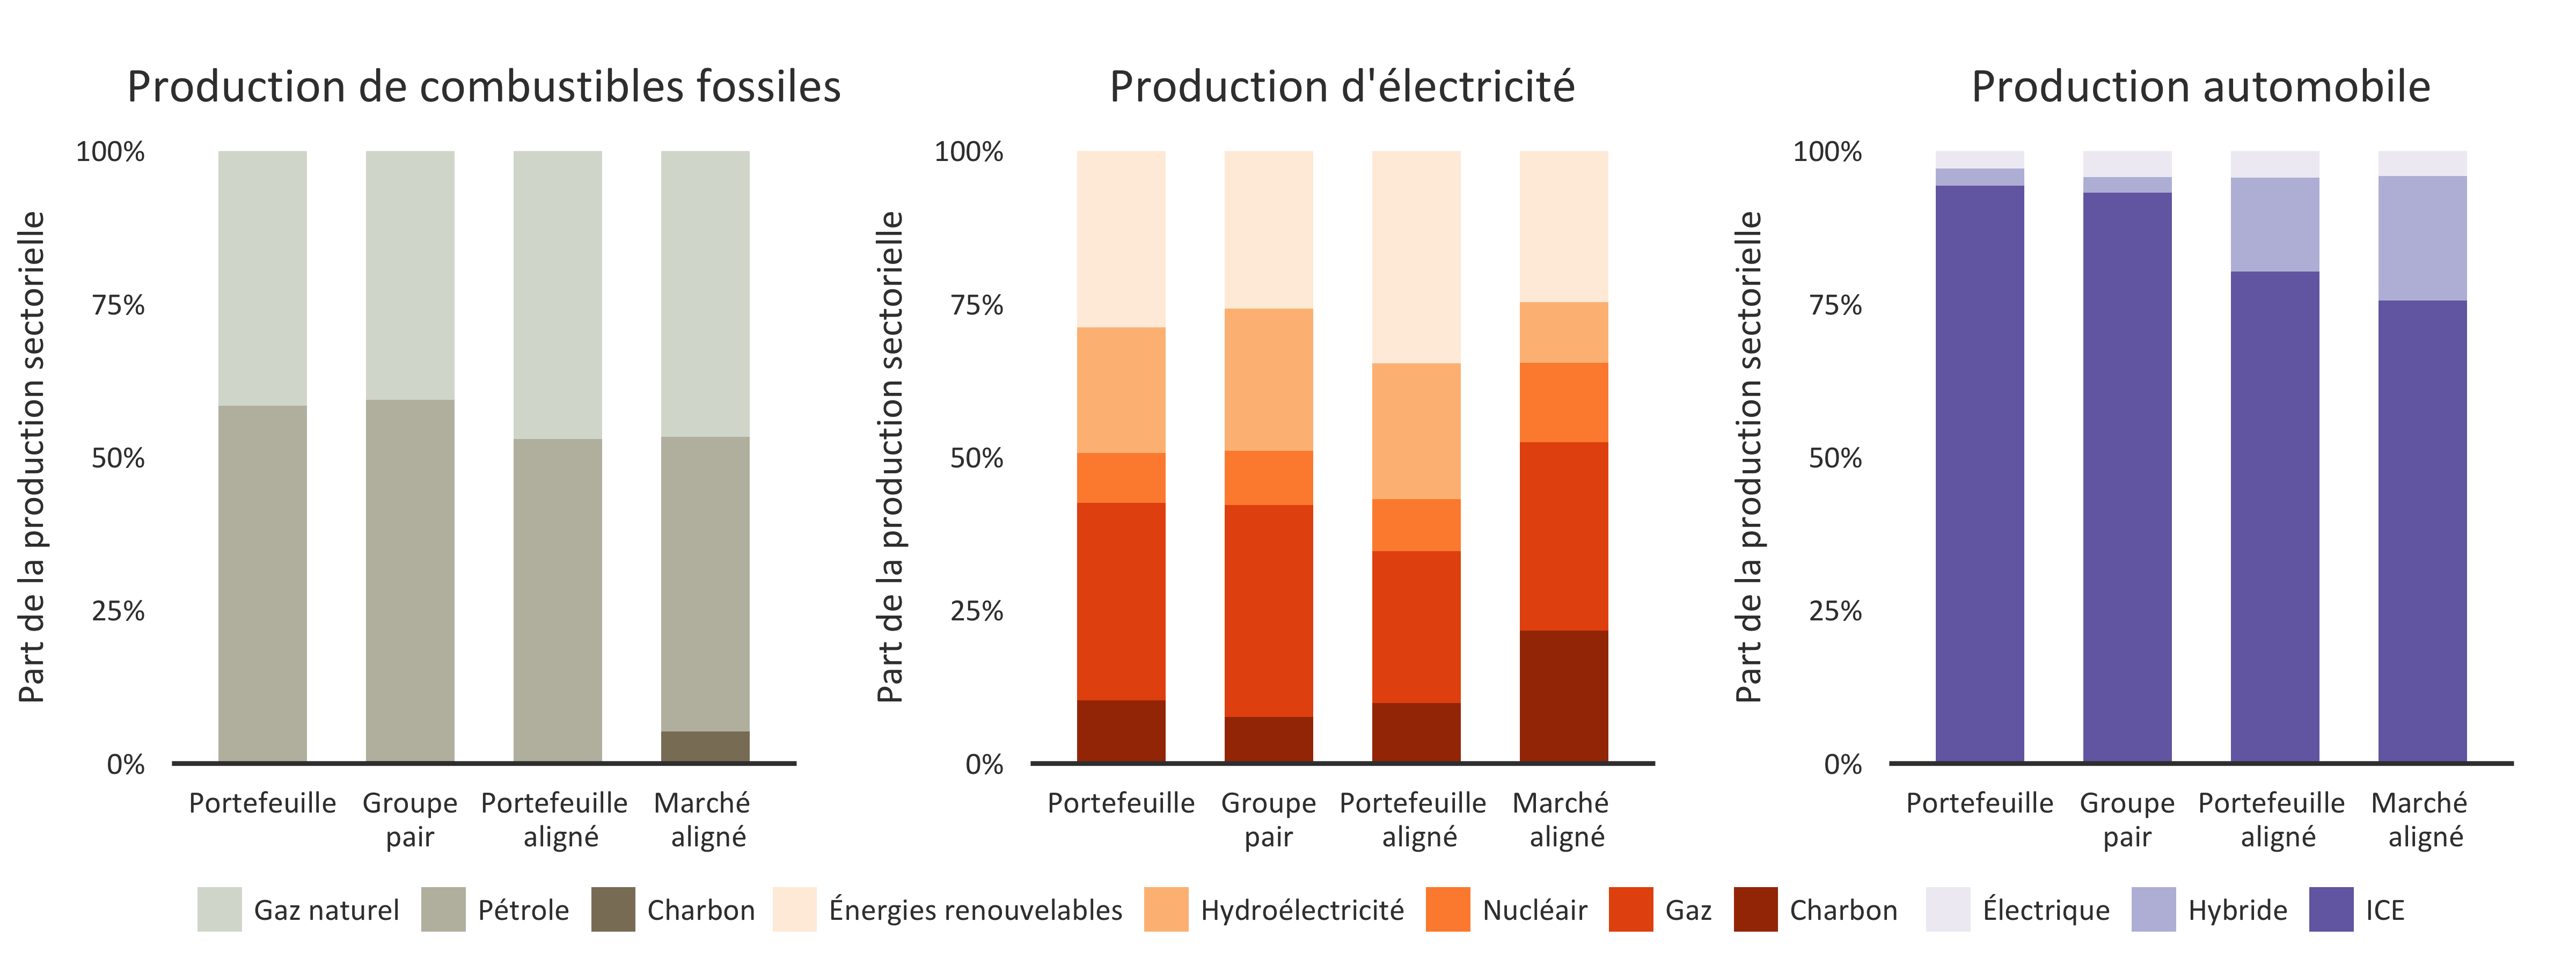
\includegraphics[trim = {0 0cm 0 0cm},width=1\linewidth]{ReportOutputs/Fig06}
	\end{center}
	%EQSpecificE
	\vspace{-0.4cm}
	\PageFooterFourth
	\newpage
	%IncRankingS
	%CBSpecificS
	\section*{} % PEER COMPARISON CB	
	\HeaderDouble{COMPARAISON AVEC LE GROUPE DE PAIRS}{OBLIGATIONS}
	

	\begin{multicols}{2}
	La figure ci-dessous résume l'écart du portefeuille d'obligations d'entreprises par rapport au ScenarioValue et fournit une comparaison avec le groupe de pairs en Startyear+5. La valeur à droite de la ligne indique un « sur-alignement » au scénario; par exemple une sur-exposition aux technologies faiblement carbonées et une sous-exposition aux technologies fortement carbonées. Les technologies à faible intensité carbone sont définies comme des technologies dont la capacité devrait augmenter sur 5 ans, comme défini par le ScenarioValue.
	\end{multicols}			
		\begin{center}
%				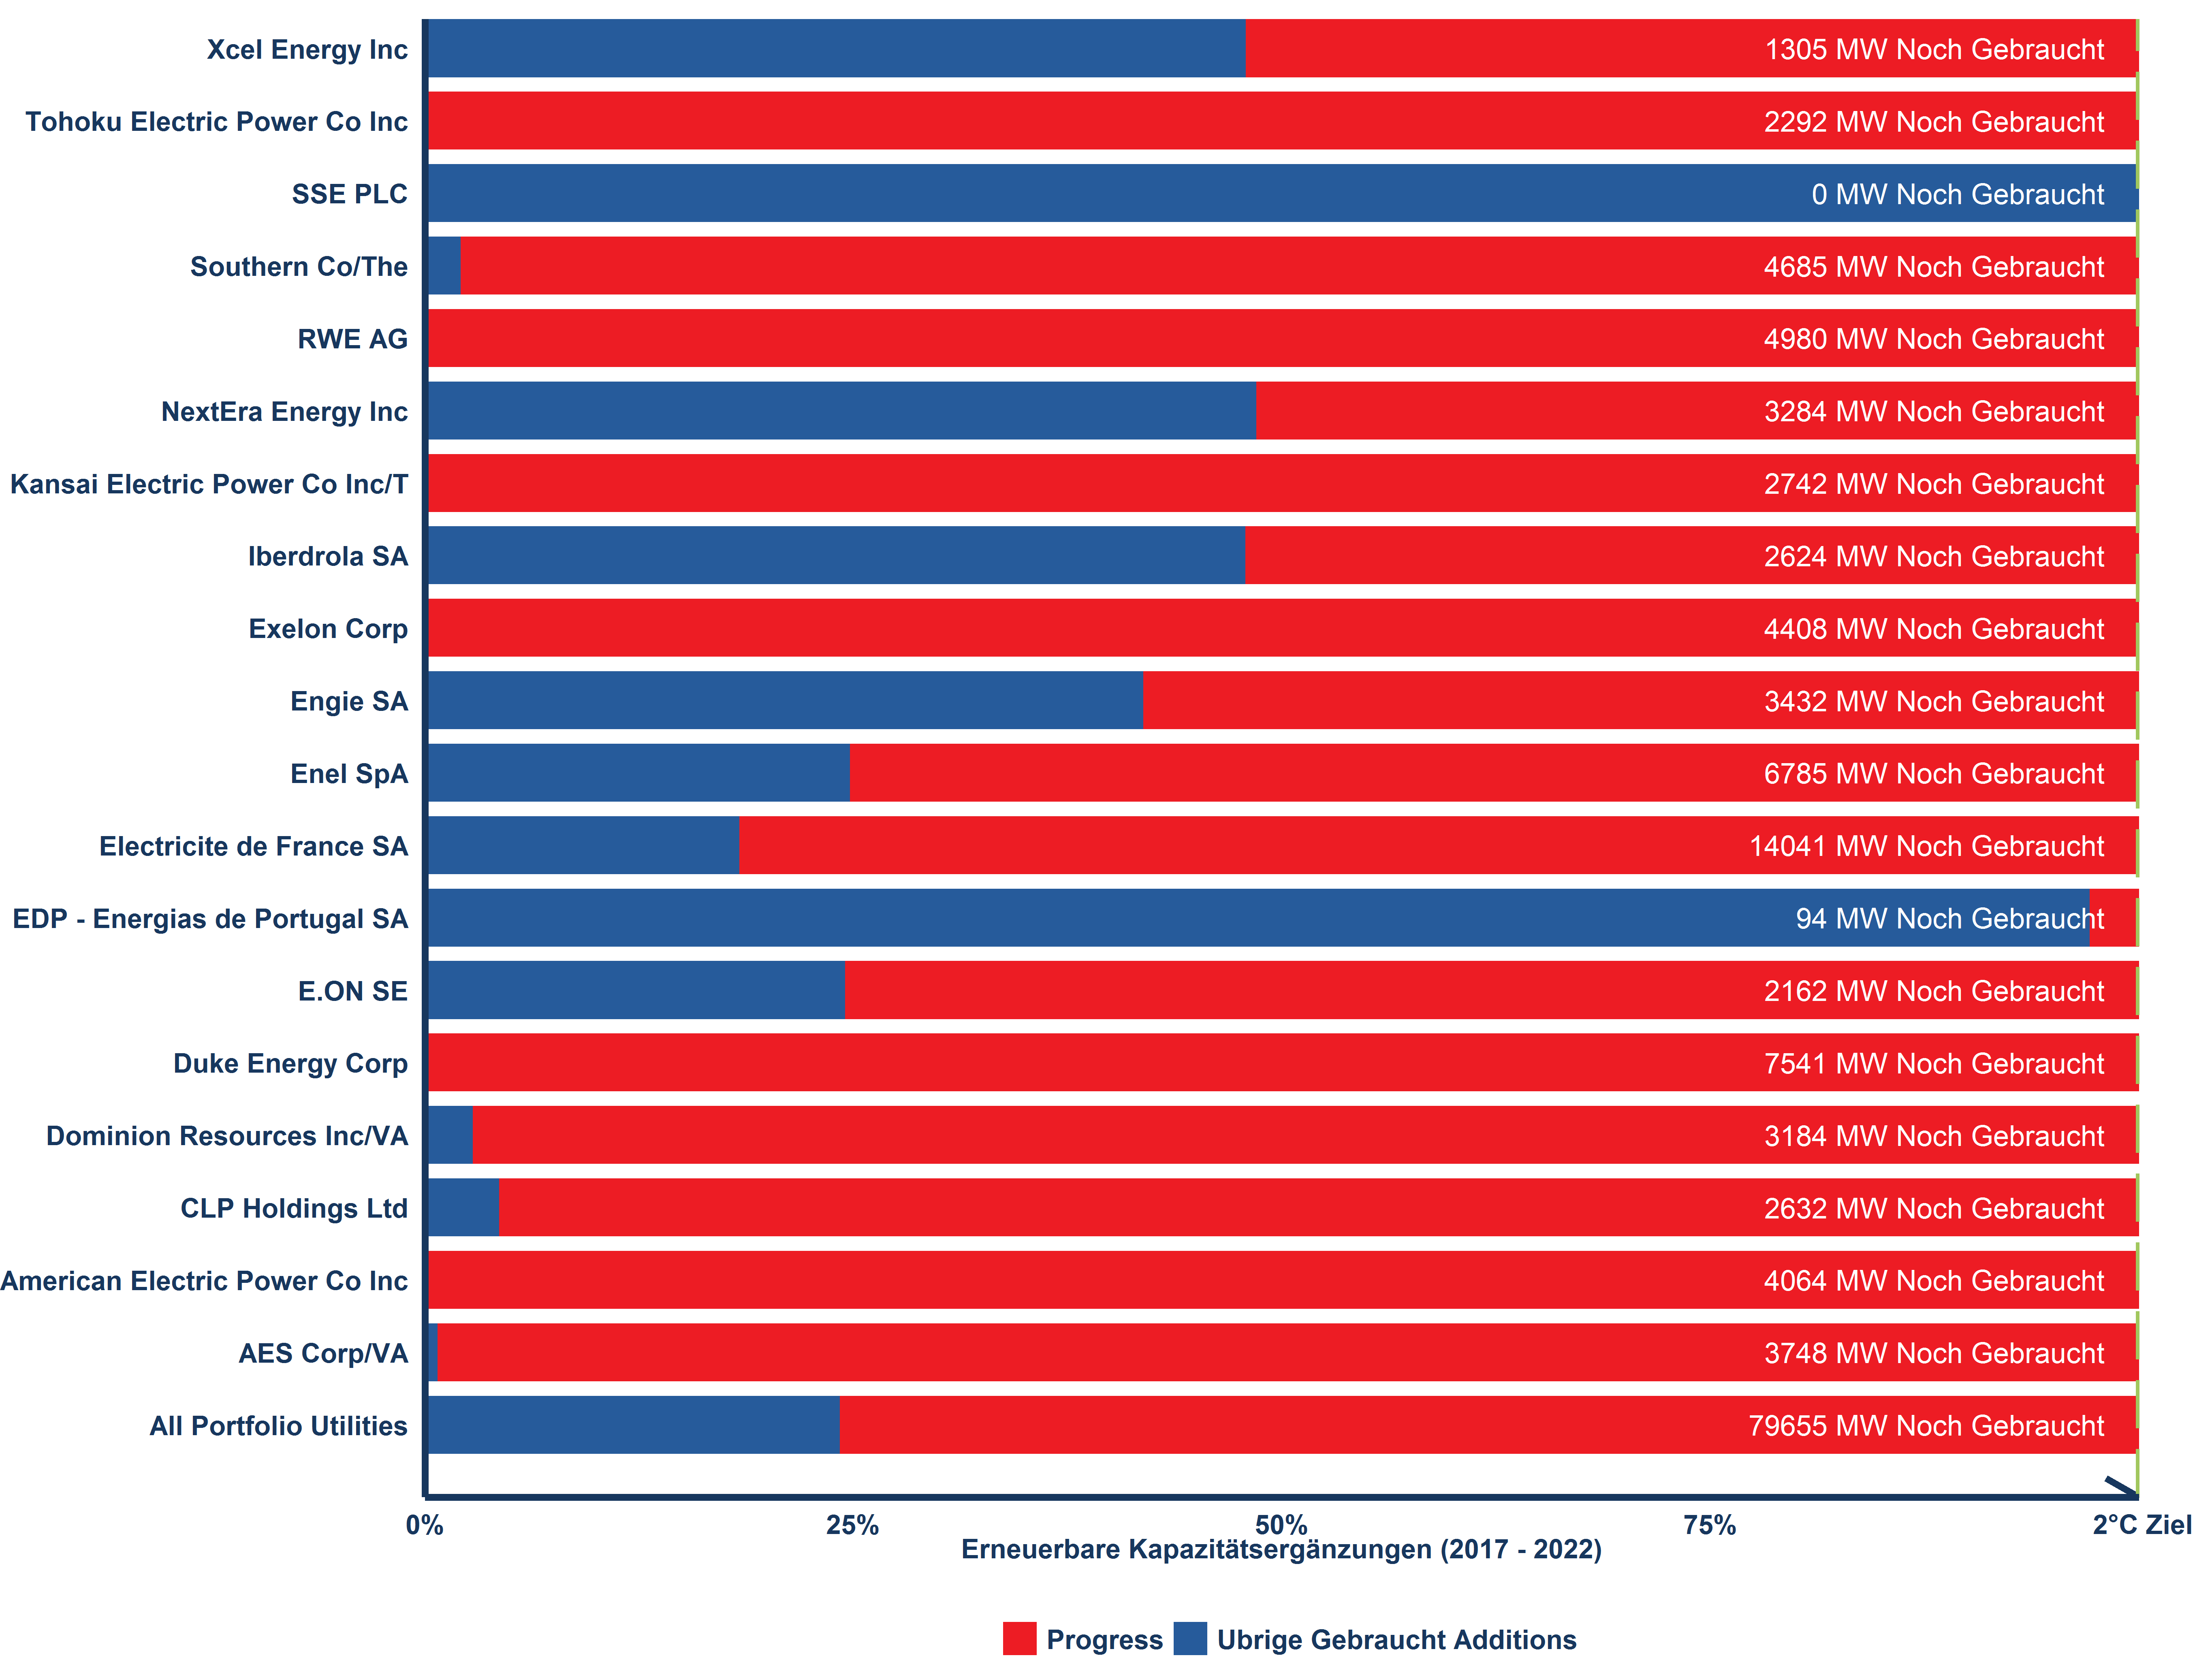
\includegraphics[trim = {0 0cm 0 0},width=1\linewidth]{ReportOutputs/Fig51}
			\end{center}		
	\PageFooterFourth
	\newpage 
	%CBSpecificE
	%EQSpecificS
	\section*{} % PEER COMPARISON EQ		
	\HeaderDouble{COMPARAISON AVEC LE GROUPE DE PAIRS}{ACTIONS}
	\begin{multicols}{2}
		La figure ci-dessous résume l'écart du portefeuille actions par rapport au ScenarioValue et fournit une comparaison avec le groupe de pairs en Startyear+5. La valeur à droite de la ligne indique un « sur-alignement » au scénario; par exemple une sur-exposition aux technologies faiblement carbonées et une sous-exposition aux technologies fortement carbonées. Les technologies à faible intensité de carbone sont définies comme des technologies dont la capacité devrait augmenter sur 5 ans, comme défini par le ScenarioValue.
	\end{multicols}	
	\begin{center}
%				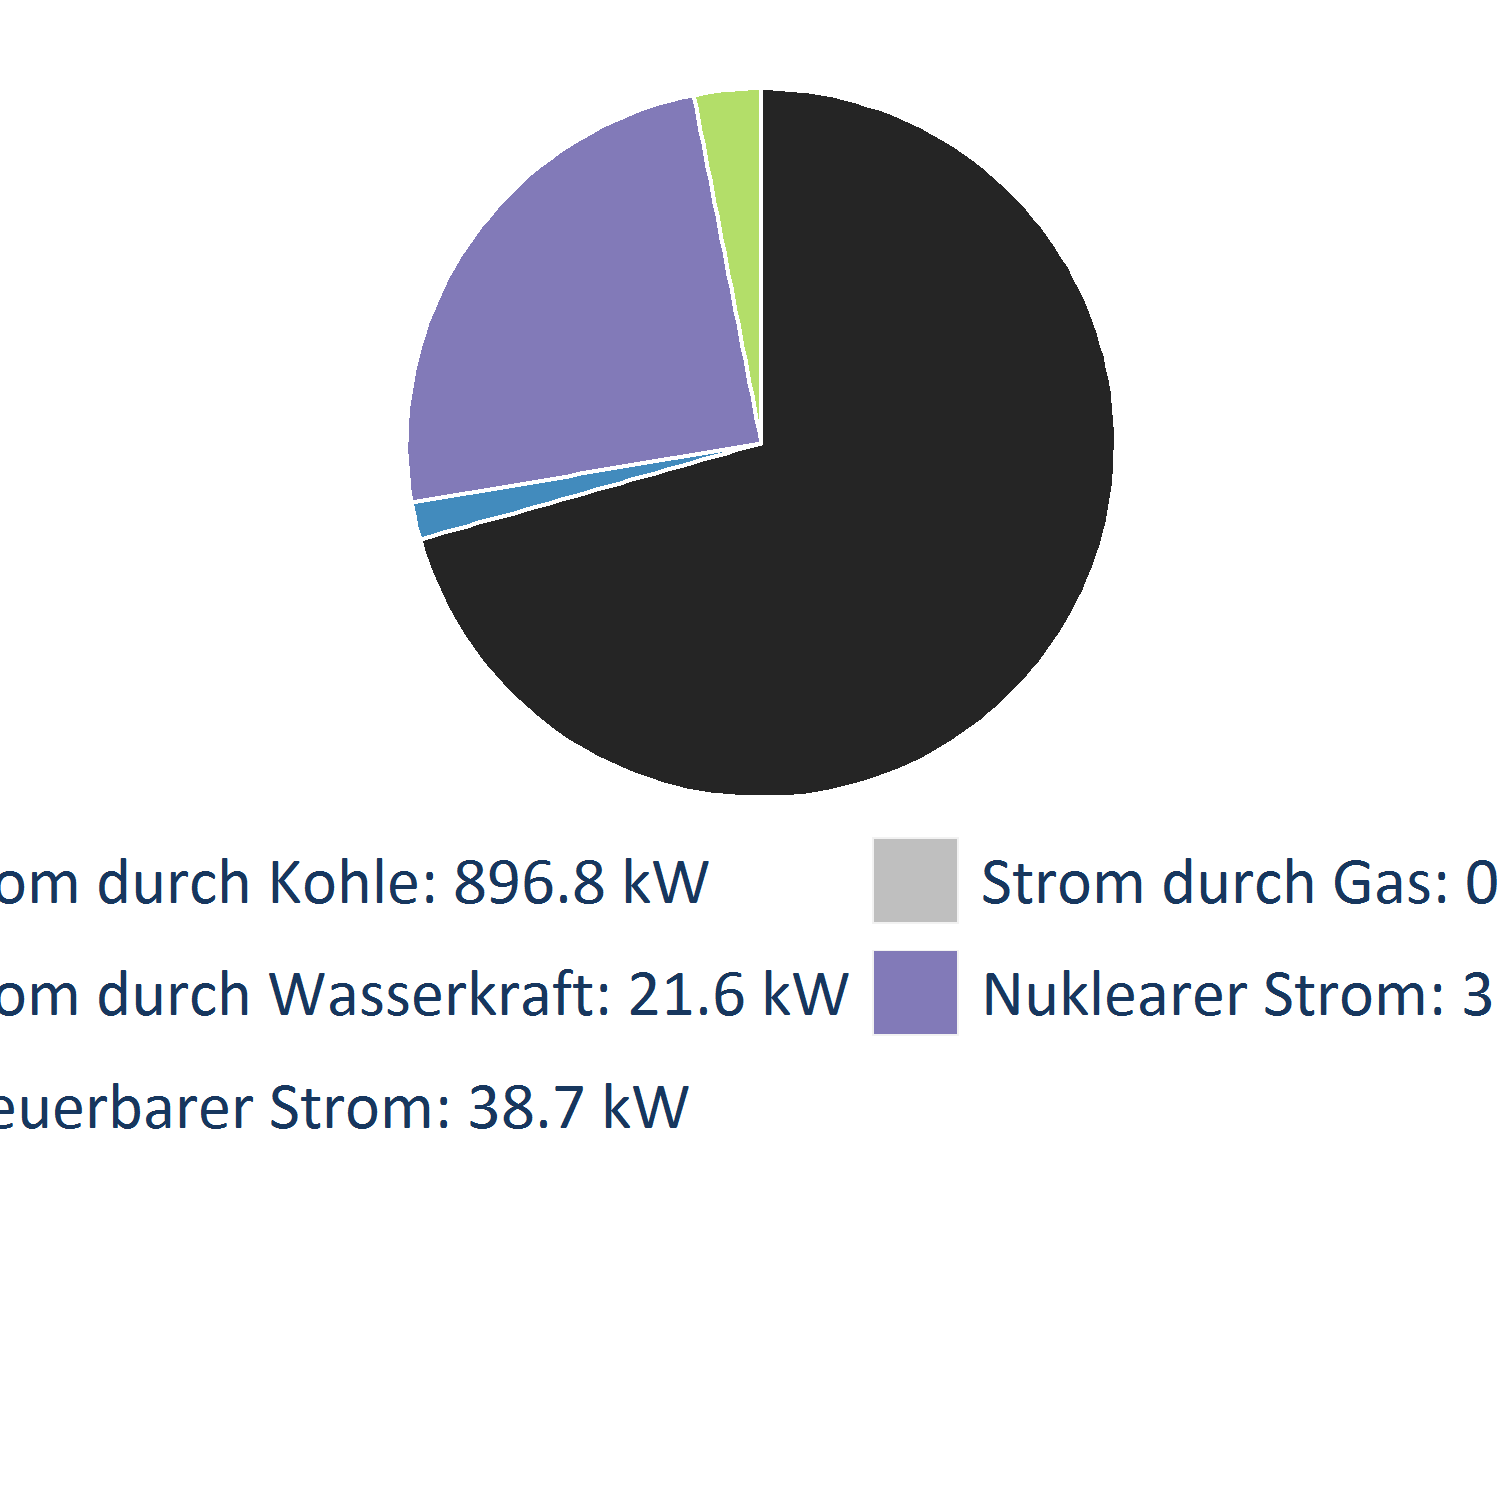
\includegraphics[trim = {0 0cm 0 0},width=1\linewidth]{ReportOutputs/Fig52}
	\end{center}		
	\PageFooterFourth
	\newpage	
	%EQSpecificE
	%IncRankingE
	%CoalMiningChartS	
	\section*{} % REGIONAL EXPOSURE		
	\HeaderDouble{EXPOSITION REGIONALE}{EXTRACTION DE CHARBON}
	
	
	Les graphiques suivants montrent l’exposition régionale des portefeuilles d’obligations d'entreprises et d’actions aux activités d’extraction de charbon en Startyear+5.
	Ceci est l’agrégation des mines de charbon allouées au portefeuille dans chaque région.
	
	%CBSpecificS
	\textbf{Exposition régionale du portefeuille d'obligations d’entreprises aux activités d'extraction de charbon}
	\vspace{-.0cm}
	
	\begin{center}
		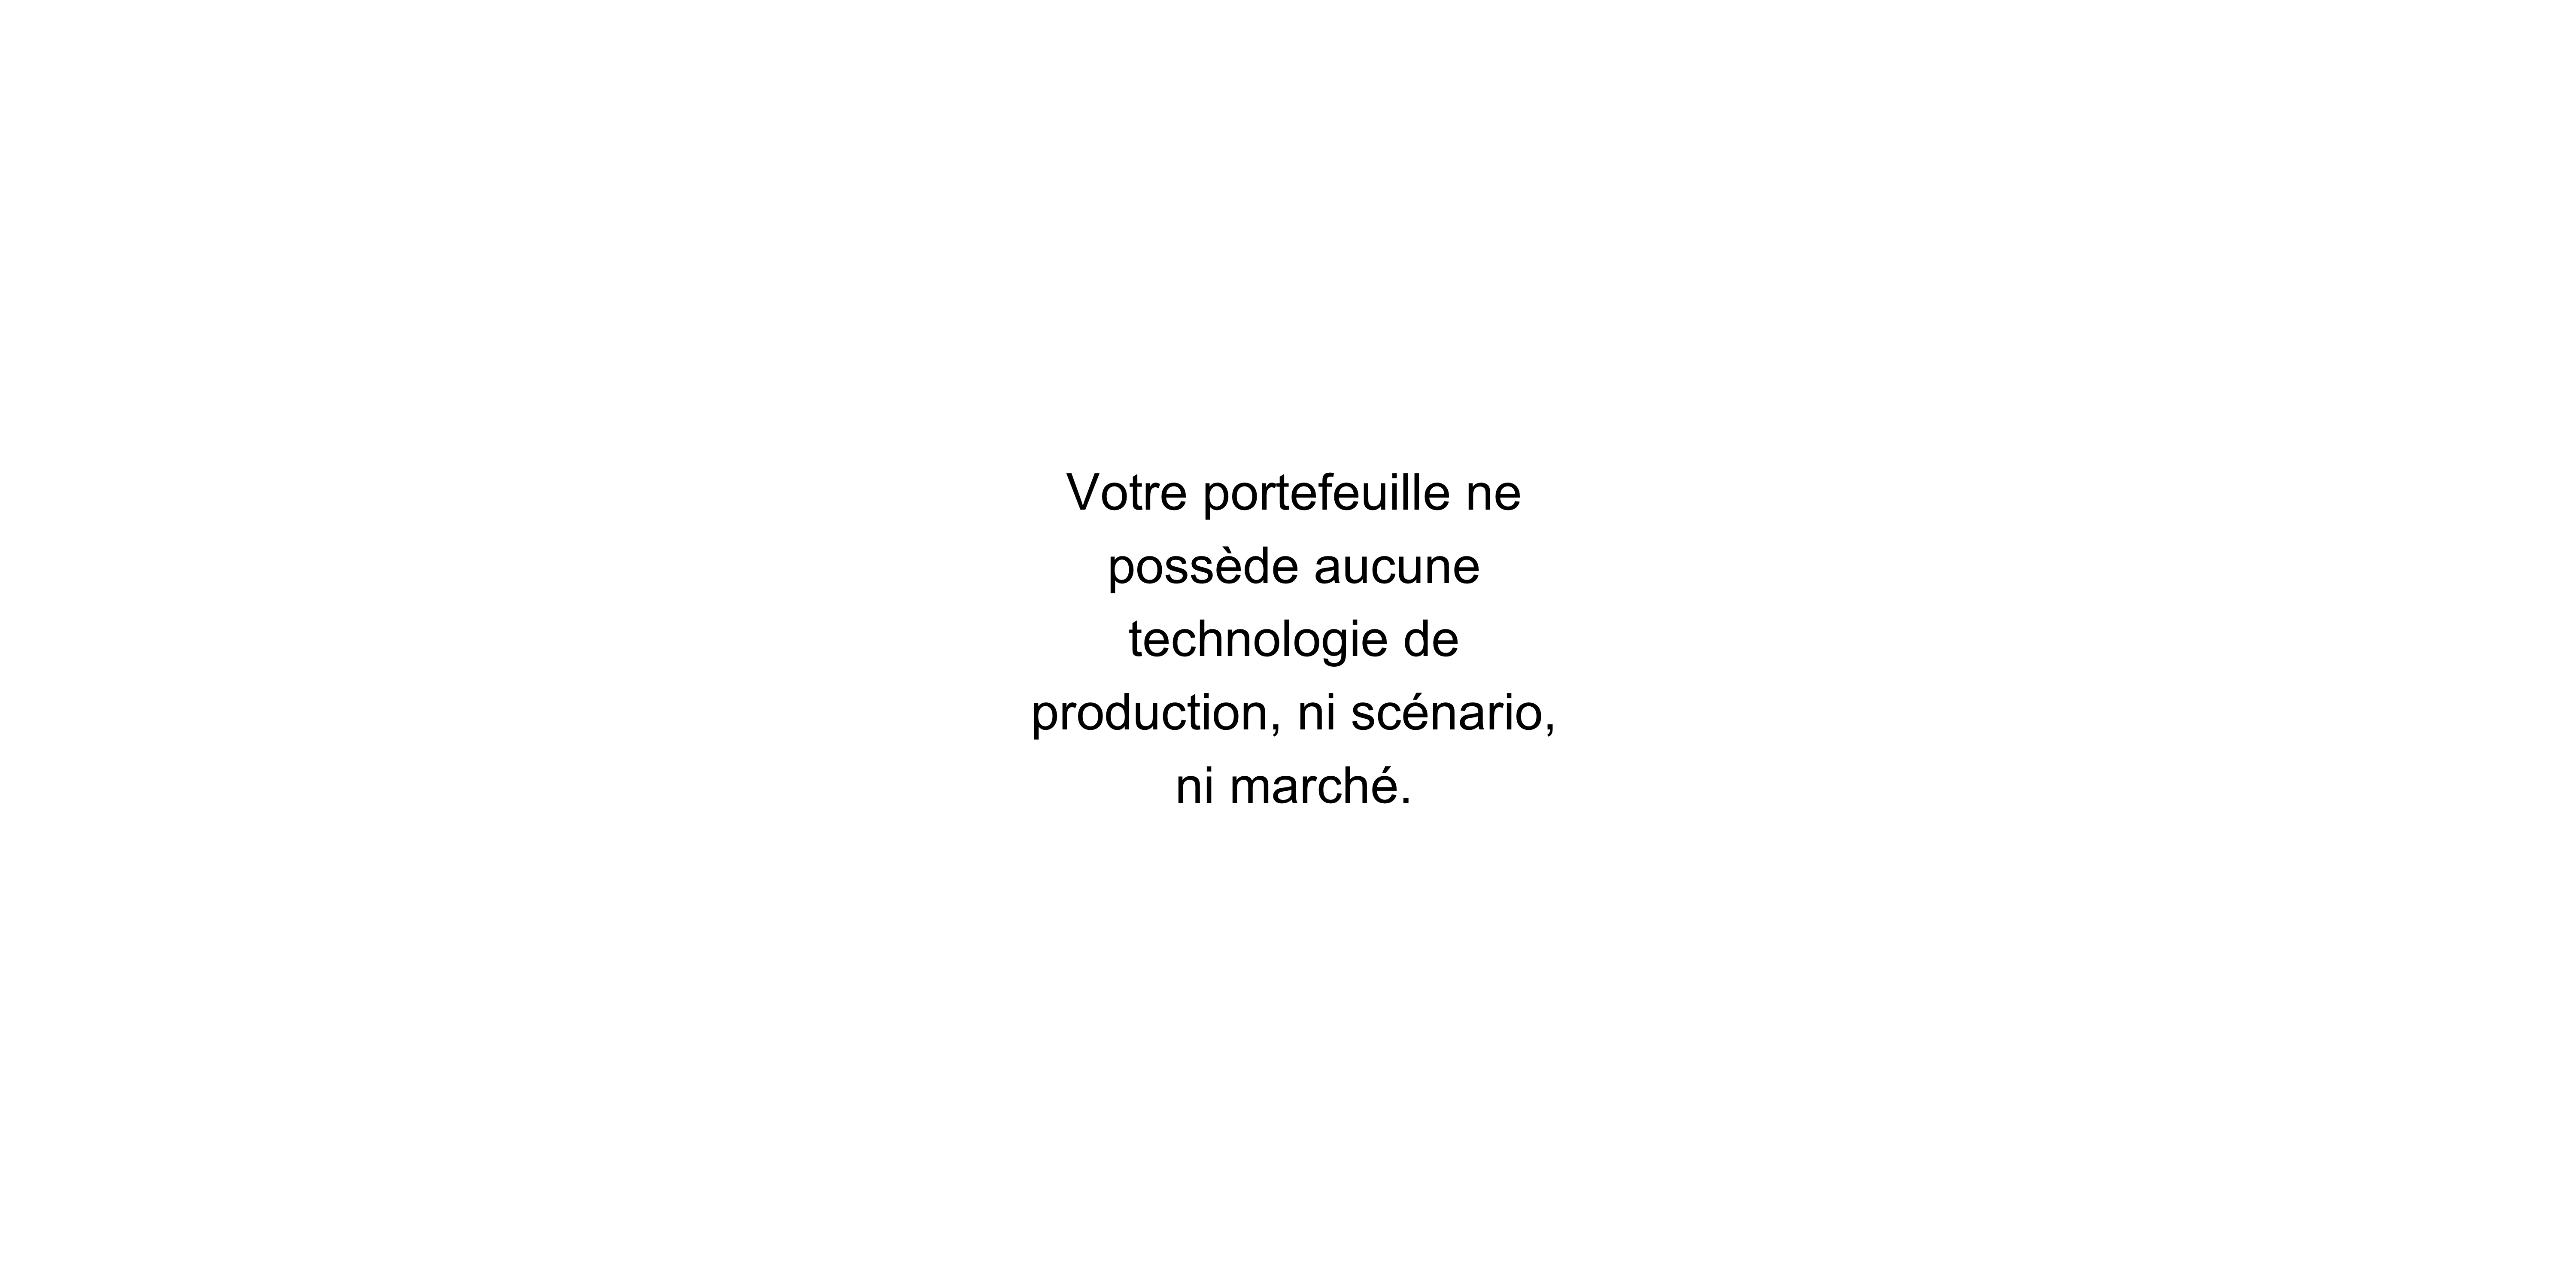
\includegraphics[trim = {2pt 2pt 2pt 2pt},clip,width=.9\linewidth]{ReportOutputs/Fig49}
	\end{center} 
	%CBSpecificE
	
	%EQSpecificS
	\textbf{Exposition régionale du portefeuille d'actions aux activités d'extraction de charbon}
	\vspace{-.0cm}
	
	\begin{center}
		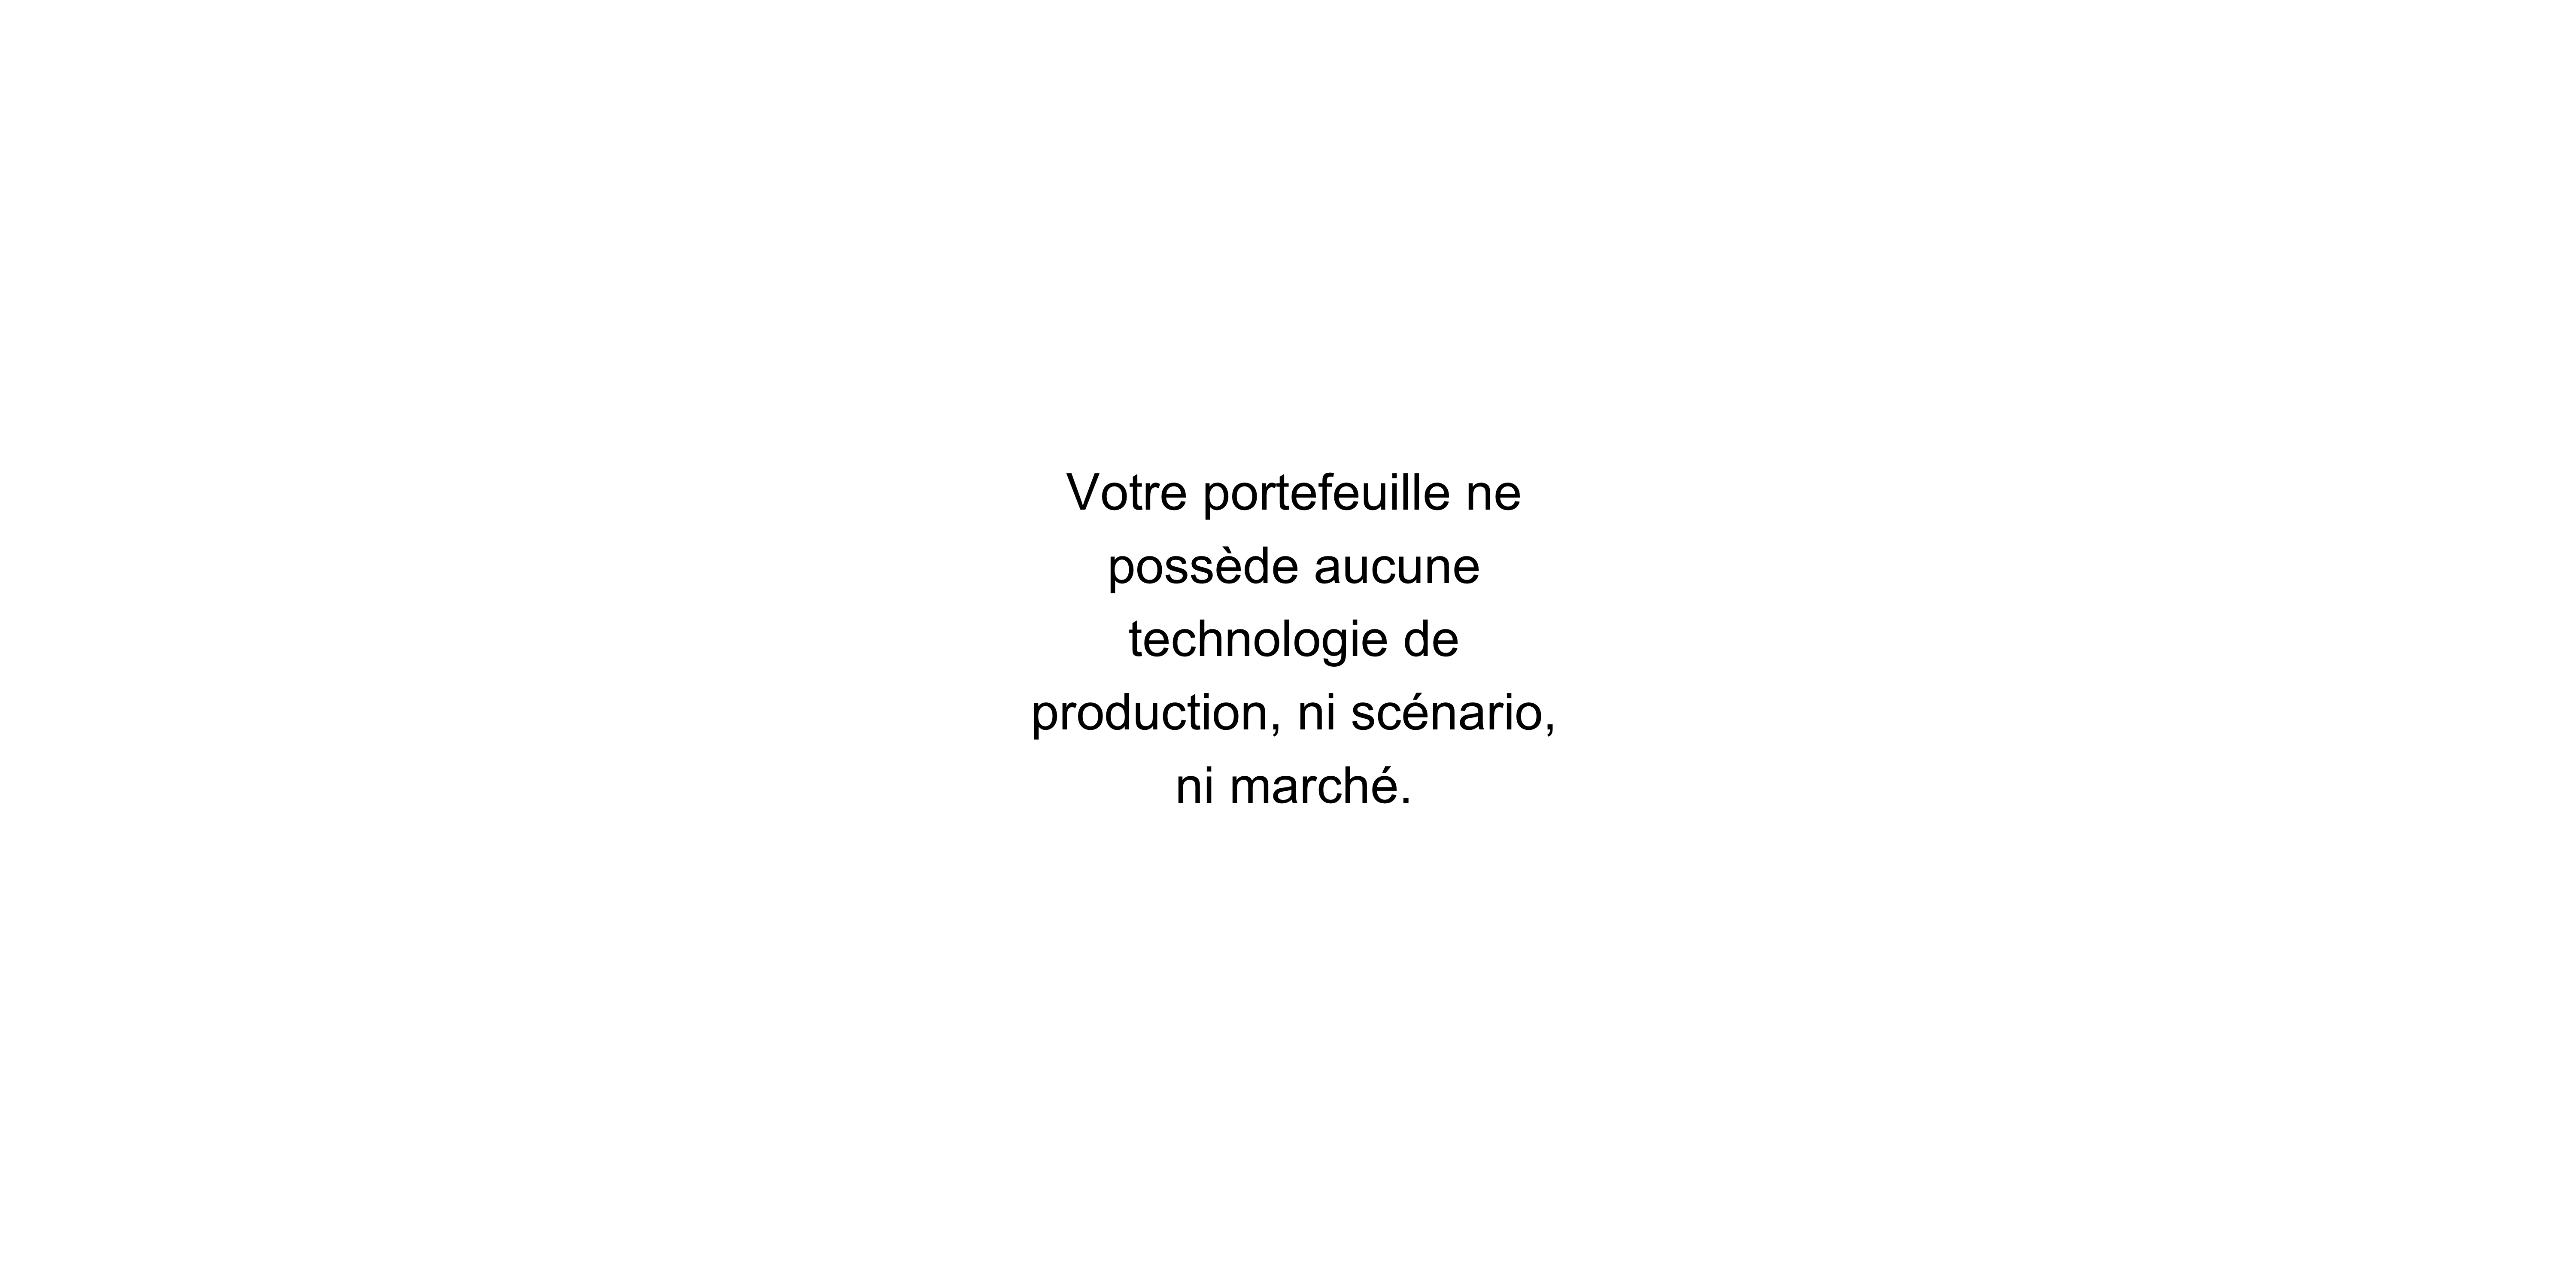
\includegraphics[trim = {1pt 1pt 1pt 1pt},width=.9\linewidth]{ReportOutputs/Fig50}
	\end{center} 
	%EQSpecificE
	
	\PageFooterFourth
	\newpage
	\section*{} % 5th SECTION   
	\SectionHeading{SECTION 5:}{EXPOSITION PAR ENTREPRISE}
	
	\newpage
	%CoalMiningChartE
	%CompanyChartsS
	\section*{} % CONTRIBUTIONS OF SECURITIES TO THE RESULTS 
	\HeaderSingle{MIX TECHNOLOGIQUE FUTUR ESTIME}
		\begin{multicols}{2}
	{\small\textbf{L'objectif de cette section est de donner un aperçu des entreprises qui contribuent le plus aux résultats présentés dans les sections précédentes.}
		
	Les pages suivantes vous montrent les résultats des différentes entreprises dans les secteurs des énergies fossiles, de l’électricité et de l’automobile. Les analyses fournies ne présentent qu'un aspect de l'analyse des scénarios potentielle des entreprises et de leur contribution à la performance d'un portefeuille. On pourrait également envisager une série d'indicateurs supplémentaires - ceux-ci dépassent la portée de ce rapport. Les indicateurs présentés ici ne doivent pas être considérés comme des recommandations d'investissement, mais plutôt comme des informations sur les entreprises à l'origine des résultats de l'analyse de scénarios. La section 6 fournit plus de détails sur les sources de données qui sous-tendent cette section.
	
		
	Dans le cadre d'un partenariat avec une équipe d'experts techniques, 2Dii développe actuellement un rapport d'analyse de scénarios d'entreprise sur le modèle des rapports de portefeuille présentés ici, conçu pour être en libre accès, dans le but de fournir une image plus complète et holistique du positionnement des entreprises face aux scénarios de transition bas carbone. Cette infrastructure pourra être utilisée pour éclairer l'analyse de portefeuille et les actions futures et sera lancée au cours du second semestre de 2019. Les analyses présentées dans ce rapport ne donnent donc qu'un aperçu du type de données qui peuvent être explorées.
	
		
	Ci-dessous se trouve un résumé sur le type d'informations présentées  pour chaque secteur présent dans le portefeuille. 
	
		
		\textbf{Secteur pétrolier et gazier.} Pour la production de pétrole et de gaz, trois types d'indicateurs sont présentés.
		
		
		\begin{enumerate}
			\item Le premier indicateur est le changement total prévu dans la production des sociétés pétrolières et gazières au cours des cinq prochaines années, d'après les plans de production divulgués actuellement dans les bases de données au niveau des actifs. Les graphiques de la page suivante montrent les plus grandes sociétés selon le volume de production de pétrole ou de gaz alloué aux portefeuilles d'obligations et d'actions en Startyear; ces sociétés sont celles qui ont le plus d'influence sur les résultats d'alignement du portefeuille dans le secteur des énergies fossiles. Pour chaque classe d'actif et chaque technologie, les résultats sont présentés par rapport à la variation totale de la production cible du portefeuille au cours de la période de cinq ans sous la rubrique SDS (barre verte). Il est à noter que les données de production fournies sont basées sur les estimations actuelles de la production et de l’évolution des actifs existants aujourd’hui.
			
			Les fusions, les acquisitions et les augmentations des dépenses en immobilisations par rapport à l'année de référence pourraient bien sûr entraîner des changements dans ces tendances au fil du temps. 
			
			\item Le deuxième indicateur s'appuie sur l'analyse menée par la Carbon Tracker Initiative en partenariat avec les Principes des Nations Unies pour l'investissement responsable (UN PRI). Cet indicateur adopte une vision à plus long terme et analyse l'alignement des entreprises avec un budget carbone de 2°C selon une perspective de structure des coûts des actifs pétroliers et gaziers. Cet indicateur diffère du premier en termes d'horizon temporel et de règles d’attribution sous-jacentes qui allouent des scénarios macroéconomiques aux acteurs microéconomiques. De plus amples informations sur la méthodologie et l'approche sont disponibles à l'adresse http://www.2degreeseparation.com/ . Cet indicateur ne peut être utilisé que pour analyser le portefeuille d'actions, car les données ne sont pas disponibles pour les obligations.
			
			\item Le troisième indicateur montre la répartition des actifs pétroliers des entreprises de chacune d'elles par type de pétrole (p. ex. pétrole classique, sables bitumineux, etc.). Wood Mackenzie (2018) explique que, même s'il est nécessaire de passer des carburants à forte teneur en carbone vers des carburants à faible teneur en carbone, une alternative transitoire serait de se détourner des méthodes spécifiques d'extraction. Le rapport ne commente pas les émissions par type d'extraction, mais des données sont disponibles à ce sujet. Il est conseillé aux investisseurs de regarder au-delà des thèmes liés aux ressources et d'examiner les variations de l'intensité d'émissions en amont pour voir comment les entreprises peuvent réduire leur empreinte carbone. Même les actifs d'un même thème peuvent avoir une intensité d'émissions différente selon leur maturité, localisation ou autres facteurs spécifiques.
			
		\end{enumerate}
			
		\textbf{Secteur électrique et automobile.} Pour les secteurs de l'énergie et de l'automobile, les informations au niveau de l'entreprise se concentrent sur le mix technologique des fournisseurs et des constructeurs automobiles dans les portefeuilles d'obligations  et d'actions, informant en particulier les résultats de la section 4. De plus amples renseignements sur les plans de construction de ces entreprises et les changements au fil du temps peuvent être fournis sur demande.
		
		%CBSpecificS
		\textit{Veuillez noter que pour le portefeuille d'obligations, les résultats sont fournis au niveau du ticker de la dette. Cela est dû au fait qu'un seul ticker de dette peut être associé à plusieurs sociétés.}
		%CBSpecificE
	}
     \end{multicols}
	\PageFooterFifth
	\newpage
	%FossilFuelSector_ALLS
	\section*{} % CONTRIBUTIONS OF SECURITIES TO THE RESULTS 
	\HeaderDouble{CONTRIBUTION PAR TITRE}{PETROLE ET GAZ - OBLIGATIONS} 
	
	%FossilFuelSector_CBS
	\vspace{-.05cm}

	\textbf{Changements prévus dans la production de pétrole et de gaz des entreprises dont la plus grande partie de la production sera attribuée au portefeuille d'obligations en Startyear+5.} Ce graphique montre les augmentations et les diminutions prévues de la production de gaz et de pétrole pour les plus grandes entreprises du secteur dans le portefeuille d'obligations d’entreprises au cours des cinq prochaines années. Cela est comparé aux changements requis selon le SDS.
	\vspace{-.15cm}

	\begin{center}
		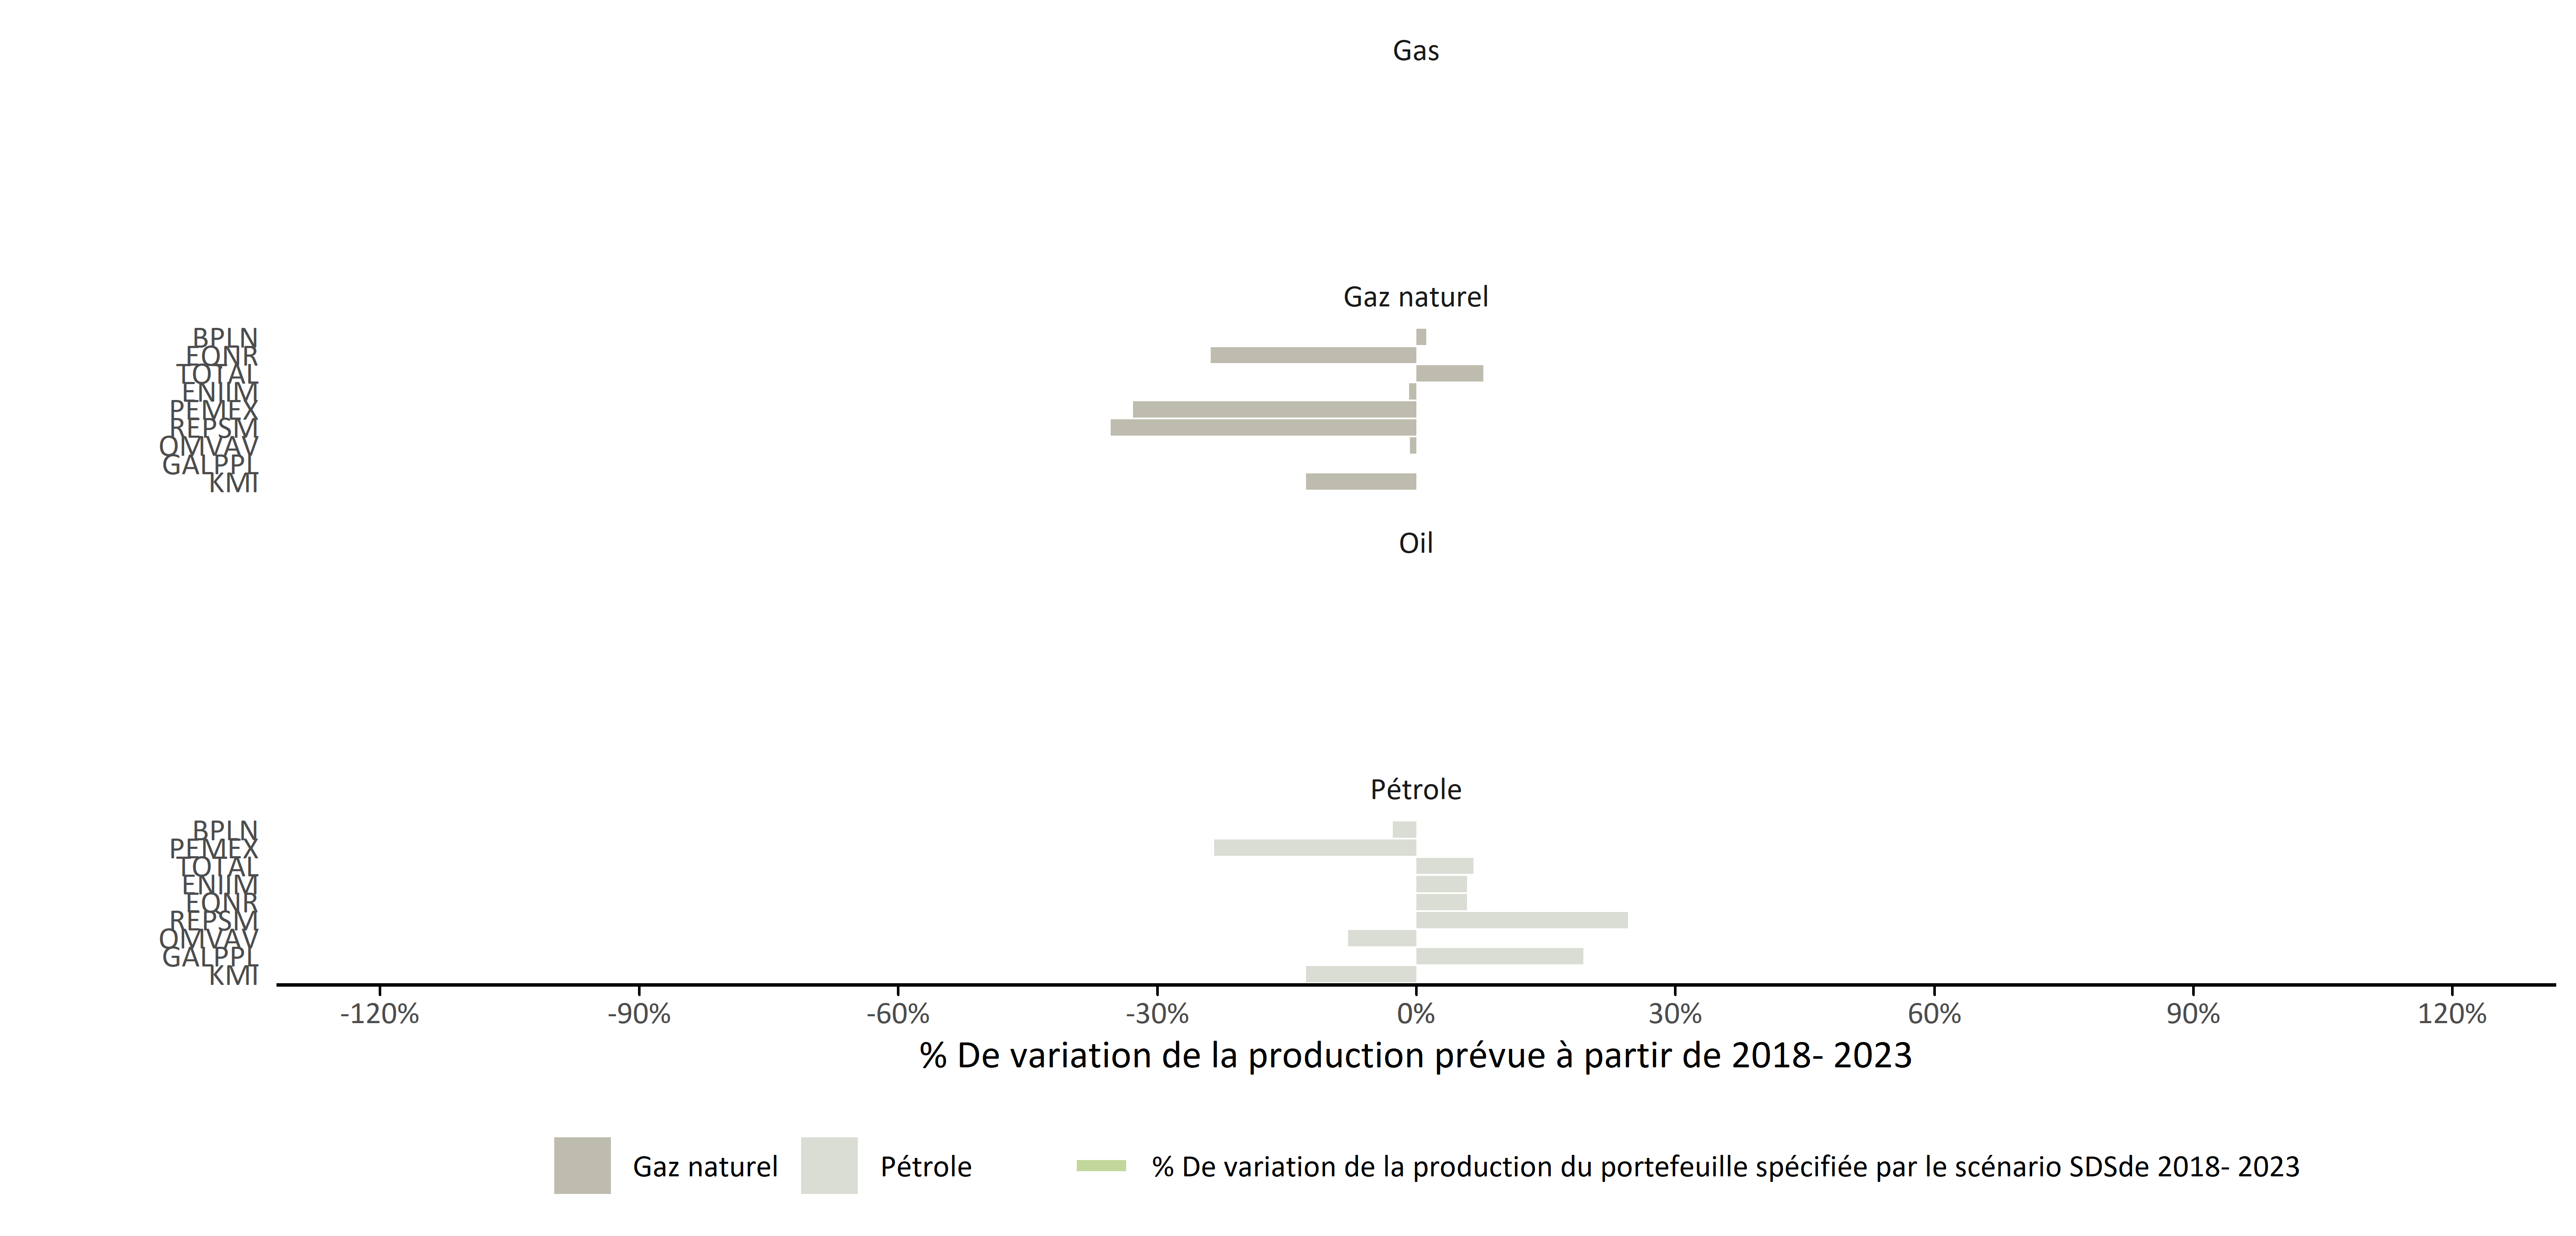
\includegraphics[trim = {0 0cm 0 0},width=1\linewidth]{ReportOutputs/Fig42}
	\end{center}

	\PageFooterFifth
	\newpage

	%FossilFuelSector_CBE
	%FossilFuelSector_EQS
	
	\section*{} % CONTRIBUTIONS OF SECURITIES TO THE RESULTS 
	\HeaderDouble{CONTRIBUTION PAR TITRE}{PETROLE ET GAZ - ACTIONS} 
	
		\textbf{Changements prévus dans la production de pétrole et de gaz des entreprises dont la plus grande partie de la production sera attribuée au portefeuille actions en  Startyear+5.} 
		
		Ce graphique montre les augmentations et les diminutions prévues de la production de gaz et de pétrole pour les plus grandes entreprises du secteur dans le portefeuille actions au cours des cinq prochaines années. Cela est comparé aux changements requis selon le SDS.
	\vspace{-.35cm}
	
	\begin{center}
		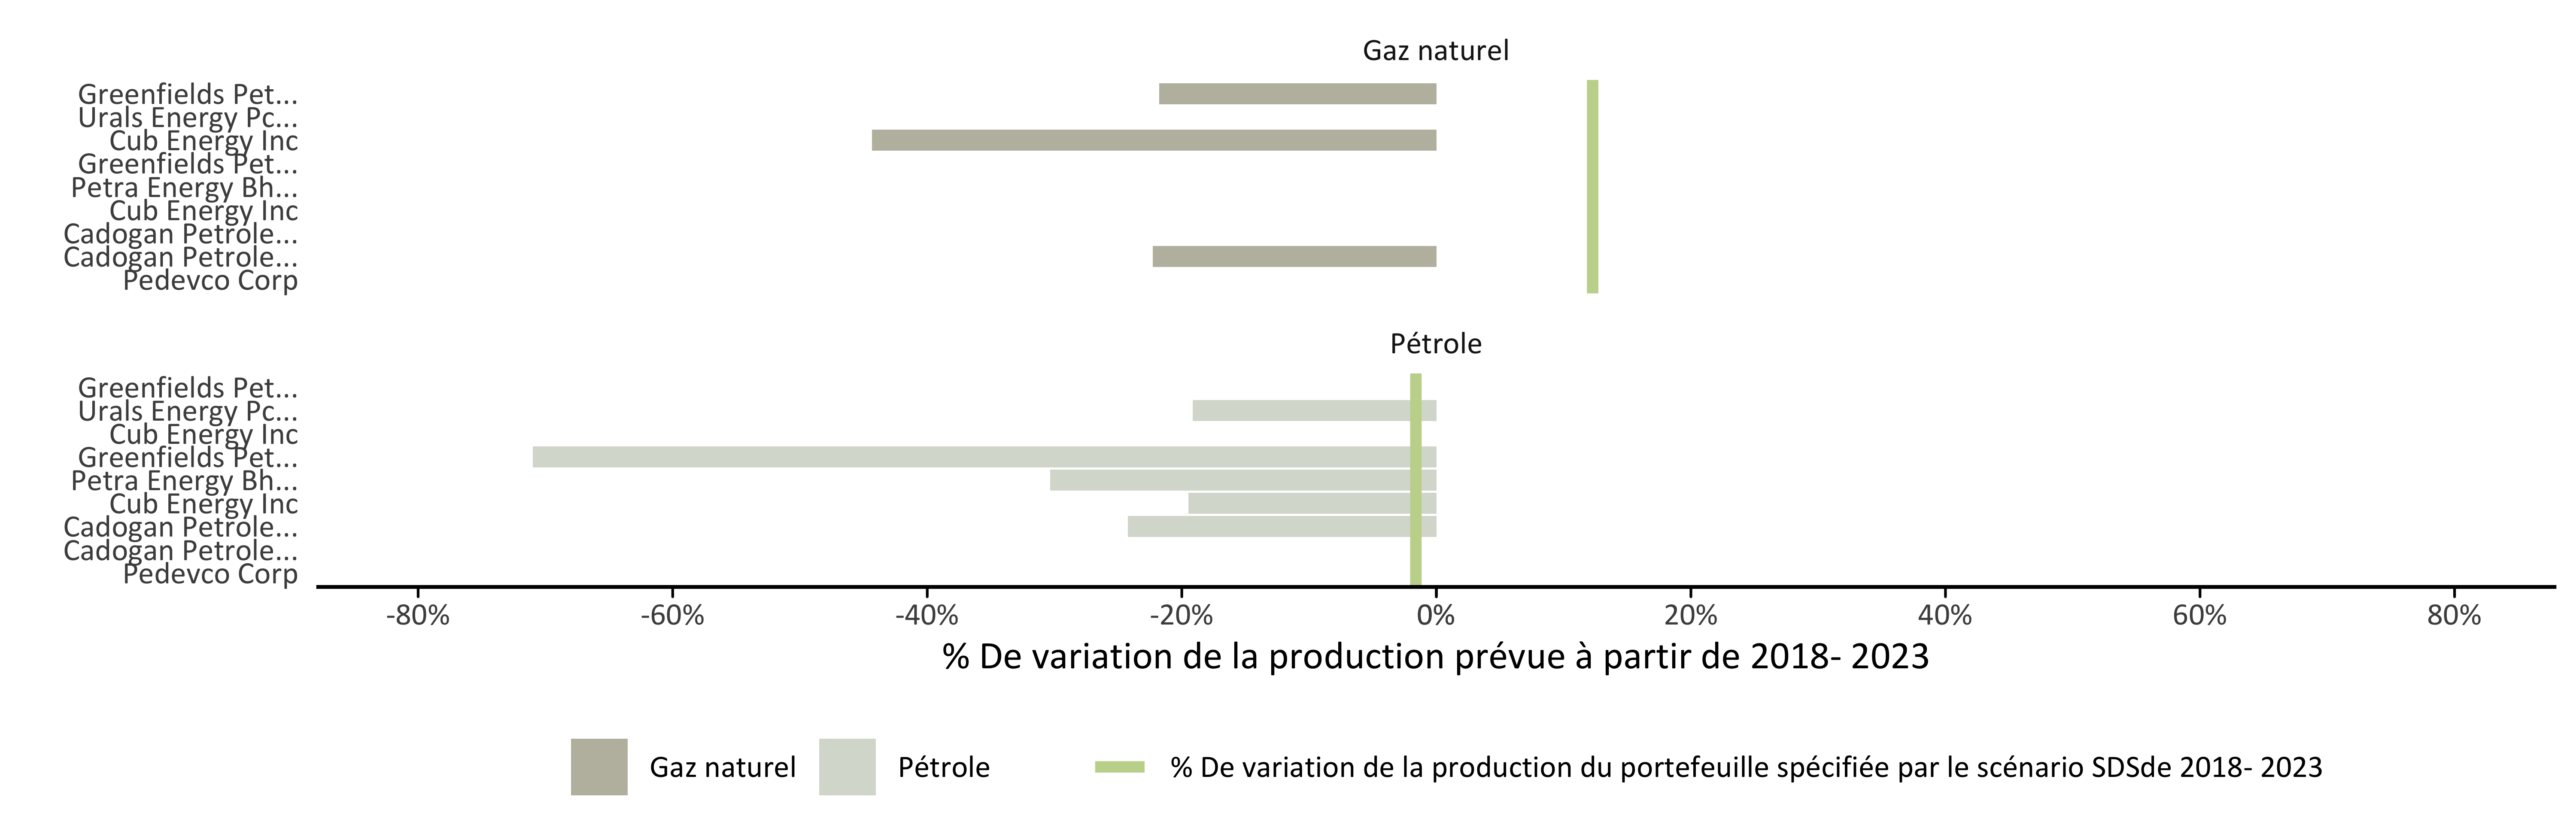
\includegraphics[trim = {0 0cm 0 0},width=1\linewidth]{ReportOutputs/Fig46}
	\end{center}
	\vspace{-.5cm}
	%\begin{center}
	%	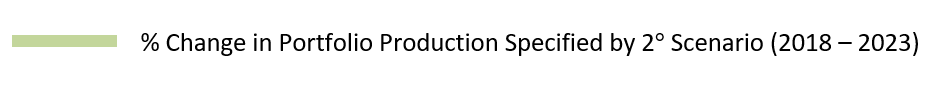
\includegraphics[trim = {0 0cm 0 0},width=.5\linewidth]{ReportGraphics/ogLegend.png}
	%\end{center}
	
	
	
	\PageFooterFifth
	\newpage
	%FossilFuelSector_EQE
	
	%CarbonBudgetS
	\section*{} % CONTRIBUTIONS OF SECURITIES TO THE RESULTS
	\HeaderDouble{CONTRIBUTION PAR TITRE}{BUDGET CARBONE}
	
	
	
	\textbf{Alignement du budget carbone des plus grosses contributions des compagnies pétrolières du portefeuille actions en  Startyear+5.}
	 
	 Ce graphique est basé sur les travaux de la Carbon Tracker Initiative et montre l'alignement du budget carbone, ainsi que par extension le niveau d'exposition potentiel aux investissements non nécessaires, des principaux producteurs de pétrole et de gaz (par valeur marchande).

	\vspace{-.35cm}
	
	\begin{center}
		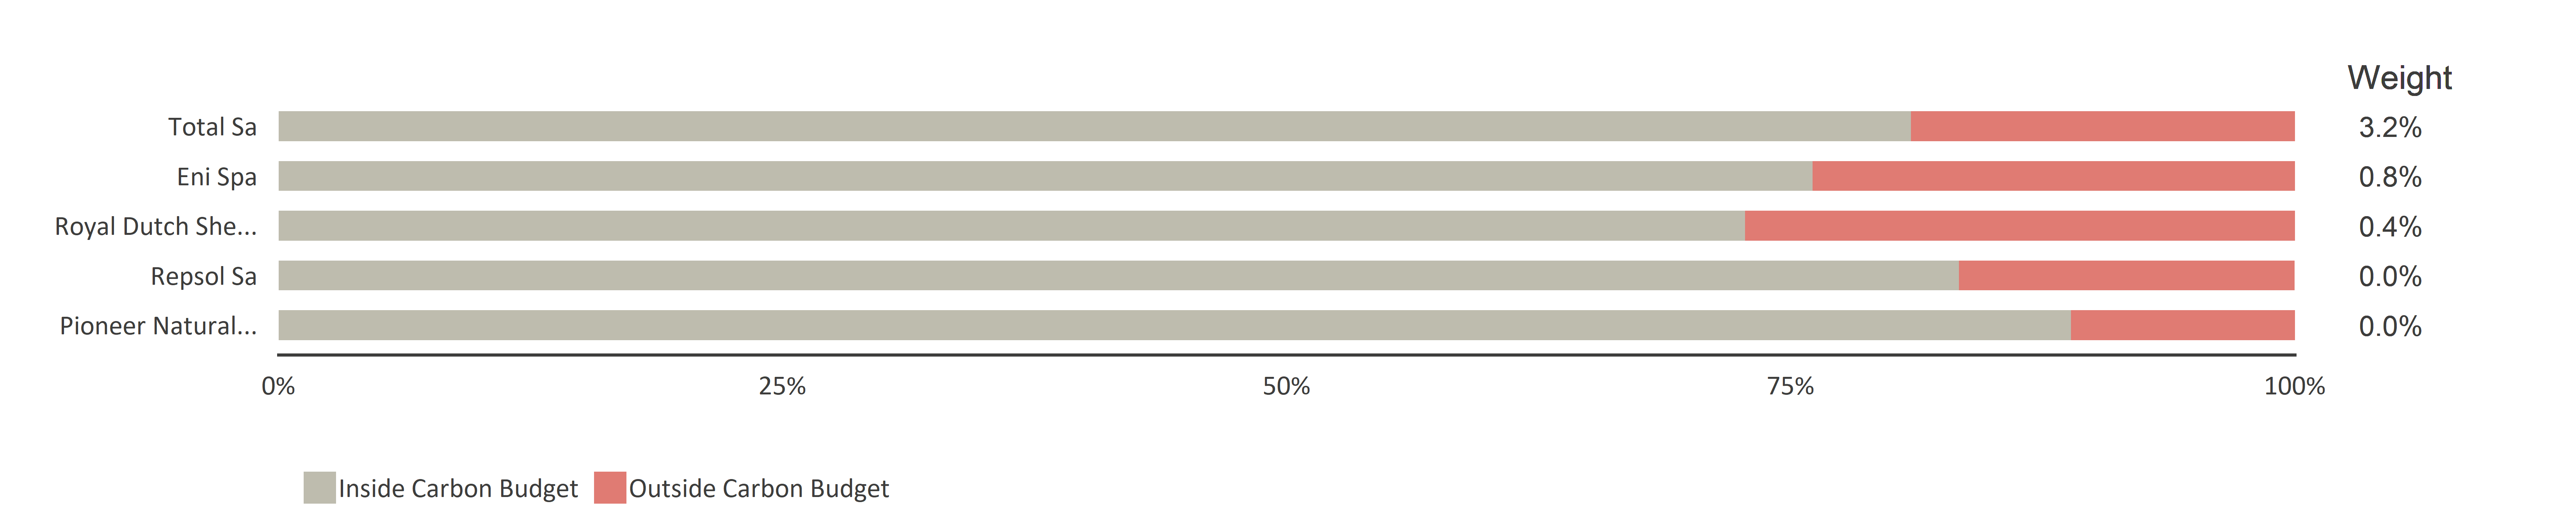
\includegraphics[trim = {0 0cm 0 0},width=1\linewidth]{ReportOutputs/Fig48}
	\end{center}

	
	\PageFooterFifth
	\newpage

	%CarbonBudgetE
	
	
	\section*{} % CONTRIBUTIONS OF SECURITIES TO THE RESULTS
	\HeaderDouble{CONTRIBUTION PAR TITRE}{PETROLE}
	
	
	%FossilFuelSector_CBS
	\textbf{Ventilation par ressources de la production de pétrole des principaux titres du portefeuille obligataire en Startyear+5.} Ce graphique montre la production de pétrole par type de pétrole pour les plus grosses contributions (en valeur marchande) des producteurs de pétrole du portefeuille obligataire en 2023.
	
	
	\vspace{-.35cm}
	
	\begin{center}
		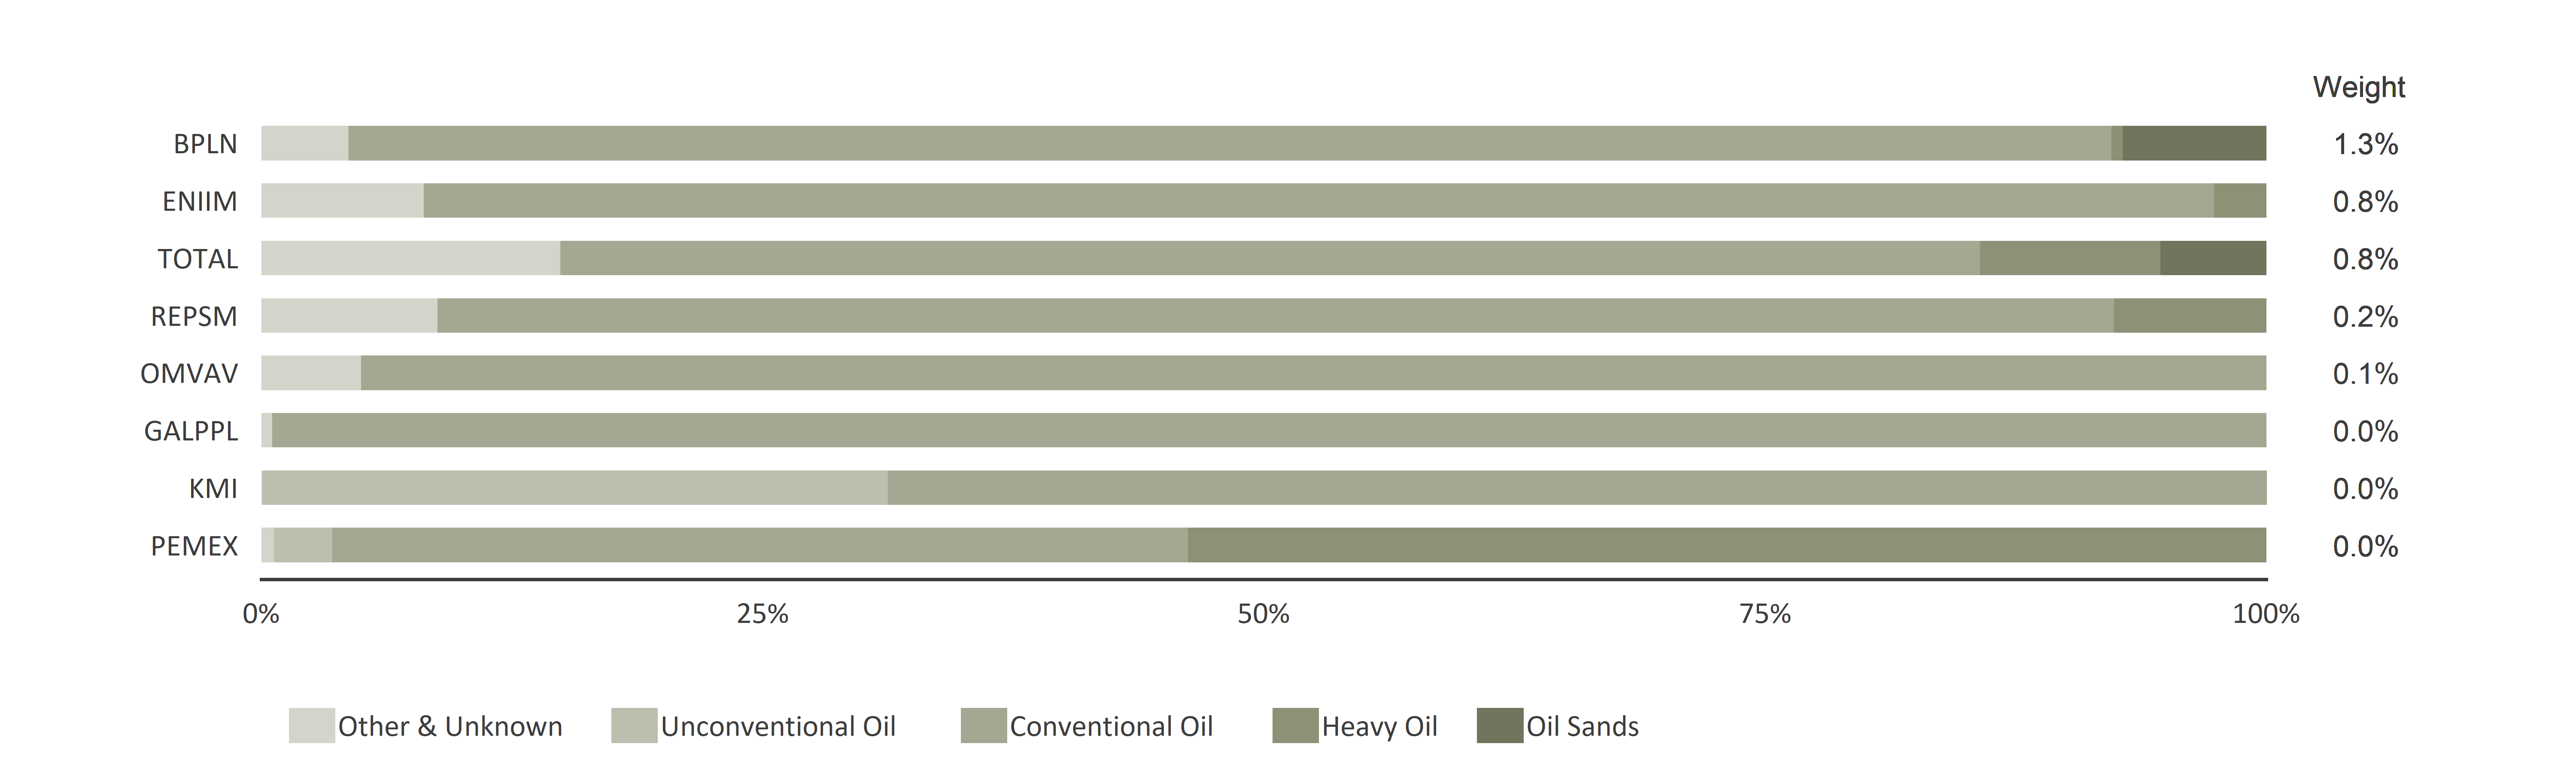
\includegraphics[trim = {0 0cm 0 0.cm},width=1\linewidth]{ReportOutputs/Fig43}
	\end{center}
	%FossilFuelSector_CBE
	
	%FossilFuelSector_EQS
	\textbf{Ventilation par ressources de la production de pétrole des principaux titres du portefeuille actions en Startyear+5.} Ce graphique montre la production de pétrole par type de pétrole pour les plus grosses contributions (en valeur marchande) des producteurs de pétrole du portefeuille actions en 2023.
	
	\vspace{-.35cm}
	
	\begin{center}
		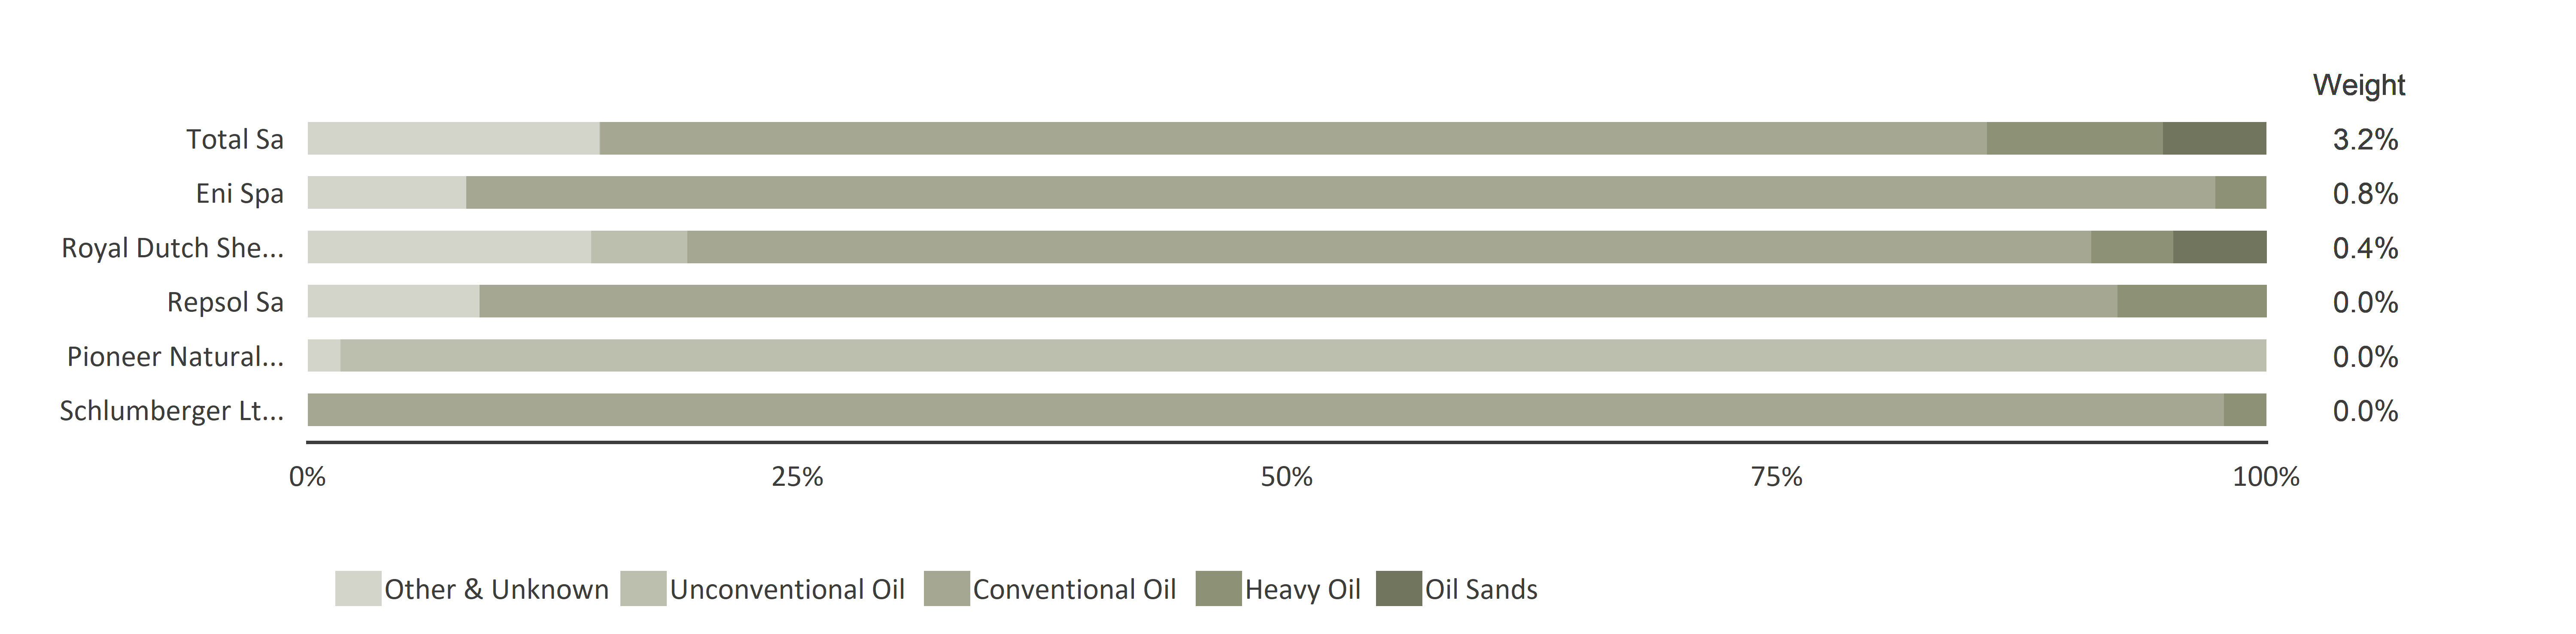
\includegraphics[trim = {0 0cm 0 0.cm},width=1\linewidth]{ReportOutputs/Fig47}
	\end{center}


	%FossilFuelSector_EQE 
	\PageFooterFifth
	\newpage

	%FossilFuelSector_ALLE
	
	
 	%PowerSector_ALLS
	\section*{} % CONTRIBUTIONS OF SECURITIES TO THE RESULTS
	%PowerAutoOneSectorS
	\HeaderDouble{CONTRIBUTION PAR TITRE}{SECTEUR ELECTRIQUE}
	%PowerAutoOneSectorE
	
	%PowerAutoTwoSectorsS
	\HeaderDouble{CONTRIBUTIONS DES INVESTISSEURS AUX RÉSULTATS}{ÉLECTRICITE AND AUTOMOBILE}
	
	
	%PowerAutoTwoSectorsE
		\textbf{Le graphique ci-dessous montre le mix énergétique estimé en Startyear+5 selon les plans d'investissements actuels, pour les plus grosses contributions (relativement au portefeuille).} 

		Les résultats présentent la combinaison technologique actuellement prévue du portefeuille, à celle du portefeuille aligné avec un SDS et celle du marché obligations aligné et à l´indice de référence actions aligné en Startyear+5. La pondération est la taille de l'investissement total dans chaque société en pourcentage de la valeur totale du portefeuille concerné.

		
	
	%PowerSector_CBS
	\textbf{Ventilation technologique des sociétés du secteur électrique dans le portefeuille d'obligations d’entreprises.}
	\vspace{-.0cm}
	
	\begin{center}
		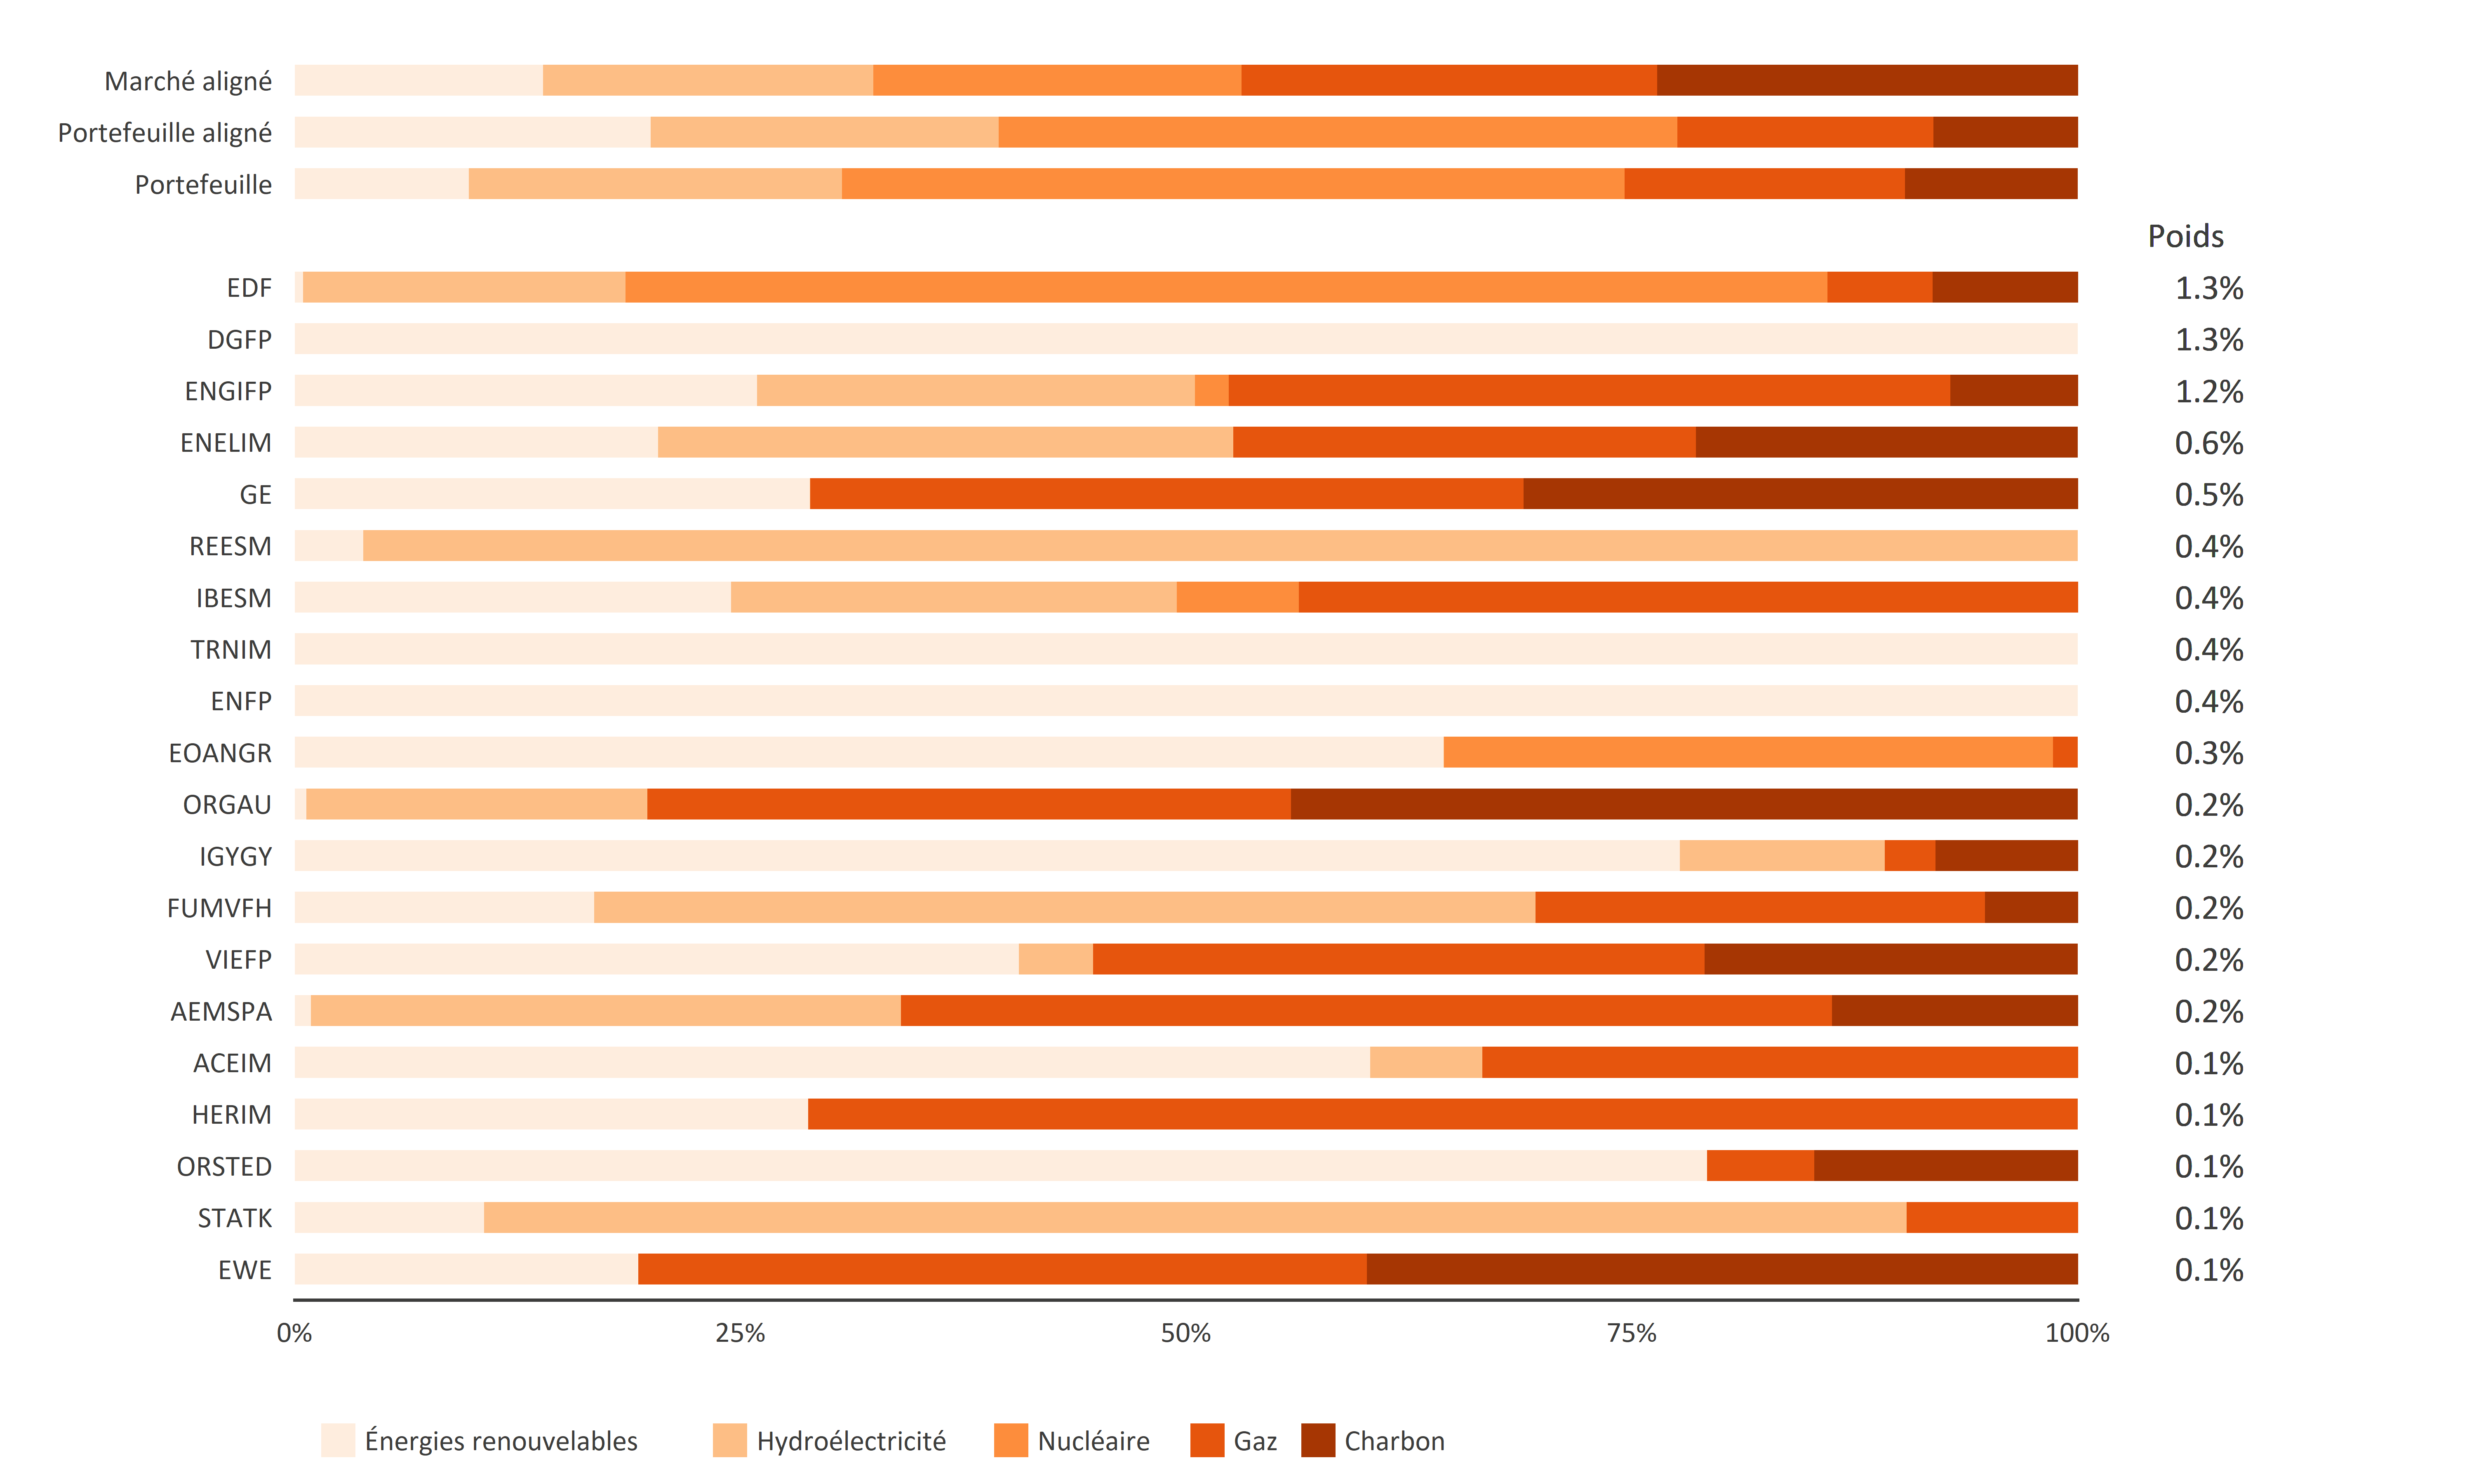
\includegraphics[trim = {0 0cm 0 0},width=1\linewidth]{ReportOutputs/Fig40}
	\end{center}
	%PowerSector_CBE
	%PowerSector_EQS
	\textbf{Ventilation technologique des sociétés du secteur électrique dans le portefeuille actions.}
	\vspace{-.0cm}
	
	\begin{center}
		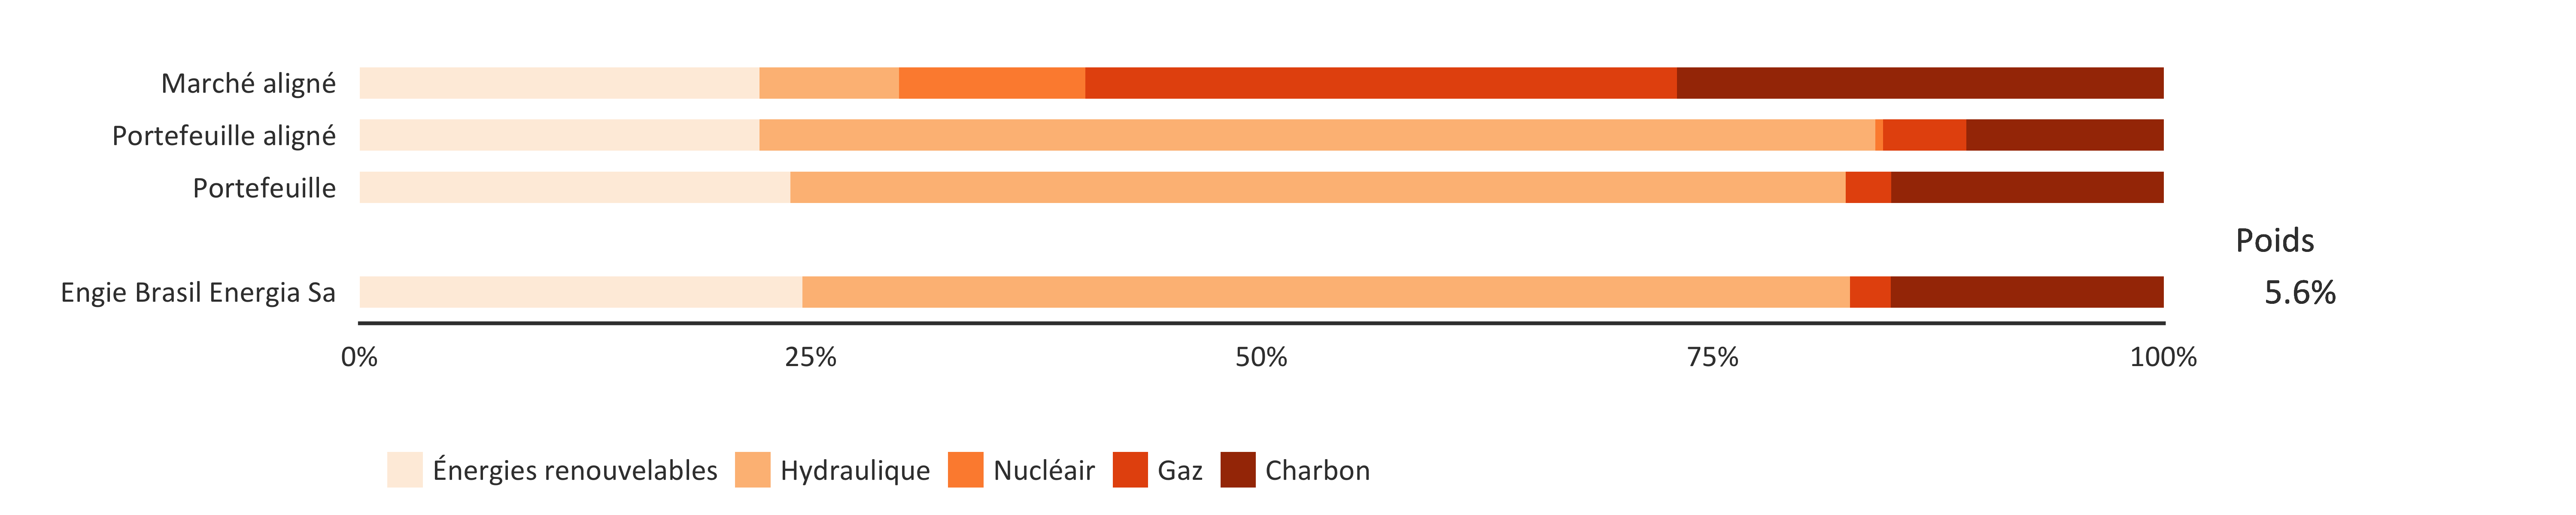
\includegraphics[trim = {0 0cm 0 0},width=1\linewidth]{ReportOutputs/Fig44}
	\end{center}		
	%PowerSector_EQE
	
	%PowerAutoOneSectorS
	\PageFooterFifth
	\newpage
	%PowerSector_ALLE
	%AutoSector_ALLS
	\section*{} % CONTRIBUTIONS OF SECURITIES TO THE RESULTS 
	\HeaderDouble{CONTRIBUTION PAR TITRE}{AUTOMOBILE}
	%PowerAutoOneSectorE
		
			\textbf{Le graphique ci-dessous montre la répartition de la production de technologies de motorisation actuellement prévue en Startyear+5 pour les plus grosses contributions du portefeuille (en valeur de marché) des entreprises du secteur.} 
		
		Les résultats présentent la combinaison technologique actuellement prévue du portefeuille, à celle du portefeuille aligné avec un SDS et celle du marché obligations aligné et à l´indice de référence actions aligné en Startyear+5. La pondération est la taille de l'investissement total dans chaque société en pourcentage de la valeur totale du portefeuille concerné.
	
	
	%AutoSector_CBS
	\textbf{Ventilation technologique des entreprises du secteur automobile dans le portefeuille d'obligations d’entreprises.}
	\vspace{-.0cm}
	
	\begin{center}
		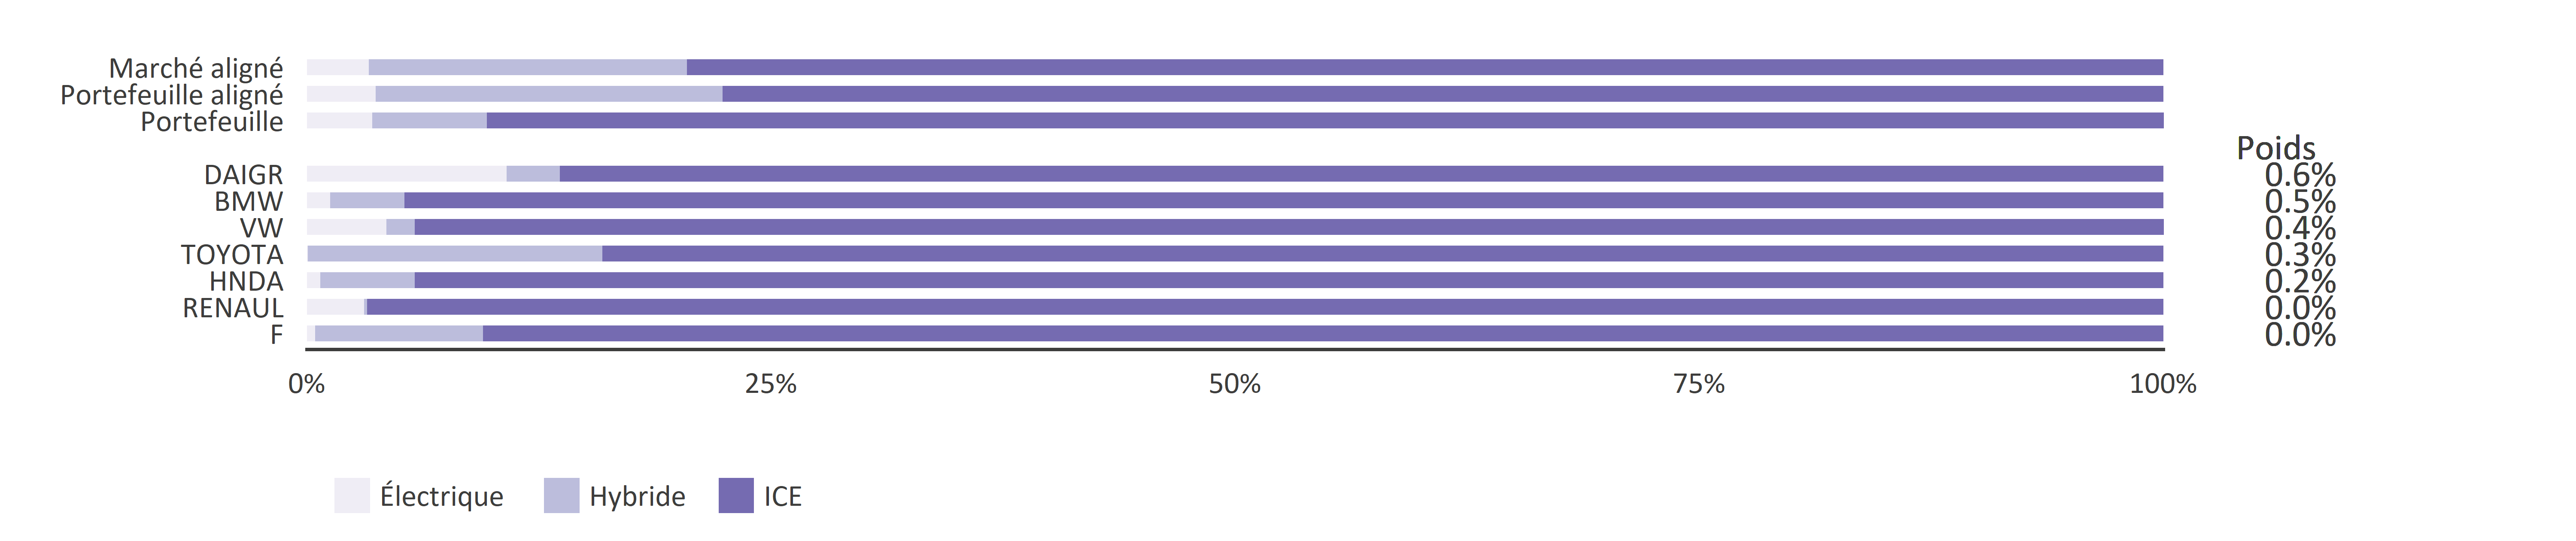
\includegraphics[trim = {0 0cm 0 0},width=1\linewidth]{ReportOutputs/Fig41}
	\end{center}
	%AutoSector_CBE
	
	%AutoSector_EQS
	\textbf{Ventilation technologique des entreprises du secteur automobile dans le portefeuille actions.}
	\vspace{-.0cm}
	
	\begin{center}
		
\includegraphics[trim = {0 0cm 0 0},width=1\linewidth]{ReportOutputs/Fig45}
	\end{center}
	%AutoSector_EQE
	
	\PageFooterFifth
	\newpage 
	%AutoSector_ALLE 
	
	%PowerSector_ALLS
	%CoalCapChartS
	\section*{} % COAL RETIREMENTS 
	\HeaderDouble{ENGAGEMENT ACTIONNARIAL}{PRODUCTION ELECTRIQUE AU CHARBON}
		
		\textbf{Le graphique suivant montre les retraits requis ainsi que les capacités additionnelles excessives des entreprises aujourd'hui dans les portefeuilles d'actions et d'obligations, pour  être alignés sur le SDS d'ici Startyear+10. }
	
    Comme la capacité devrait diminuer dans le cadre du ScenarioValue, toute nouvelle capacité installée devrait être mise hors service par le retrait de la capacité existante, ce qui est représenté par la capacité supplémentaire (en noir). Les retraits requis représentent la capacité existante qui doit être retirée en plus de la non mise en service de capacité supplémentaire.
  
	
	%CBSpecificS
	\textbf{Mises hors service et ajouts de capacités de production de charbon des entreprises dans le portefeuille d'obligations d’entreprises}
	\vspace{-.0cm}
	
	\begin{center}
		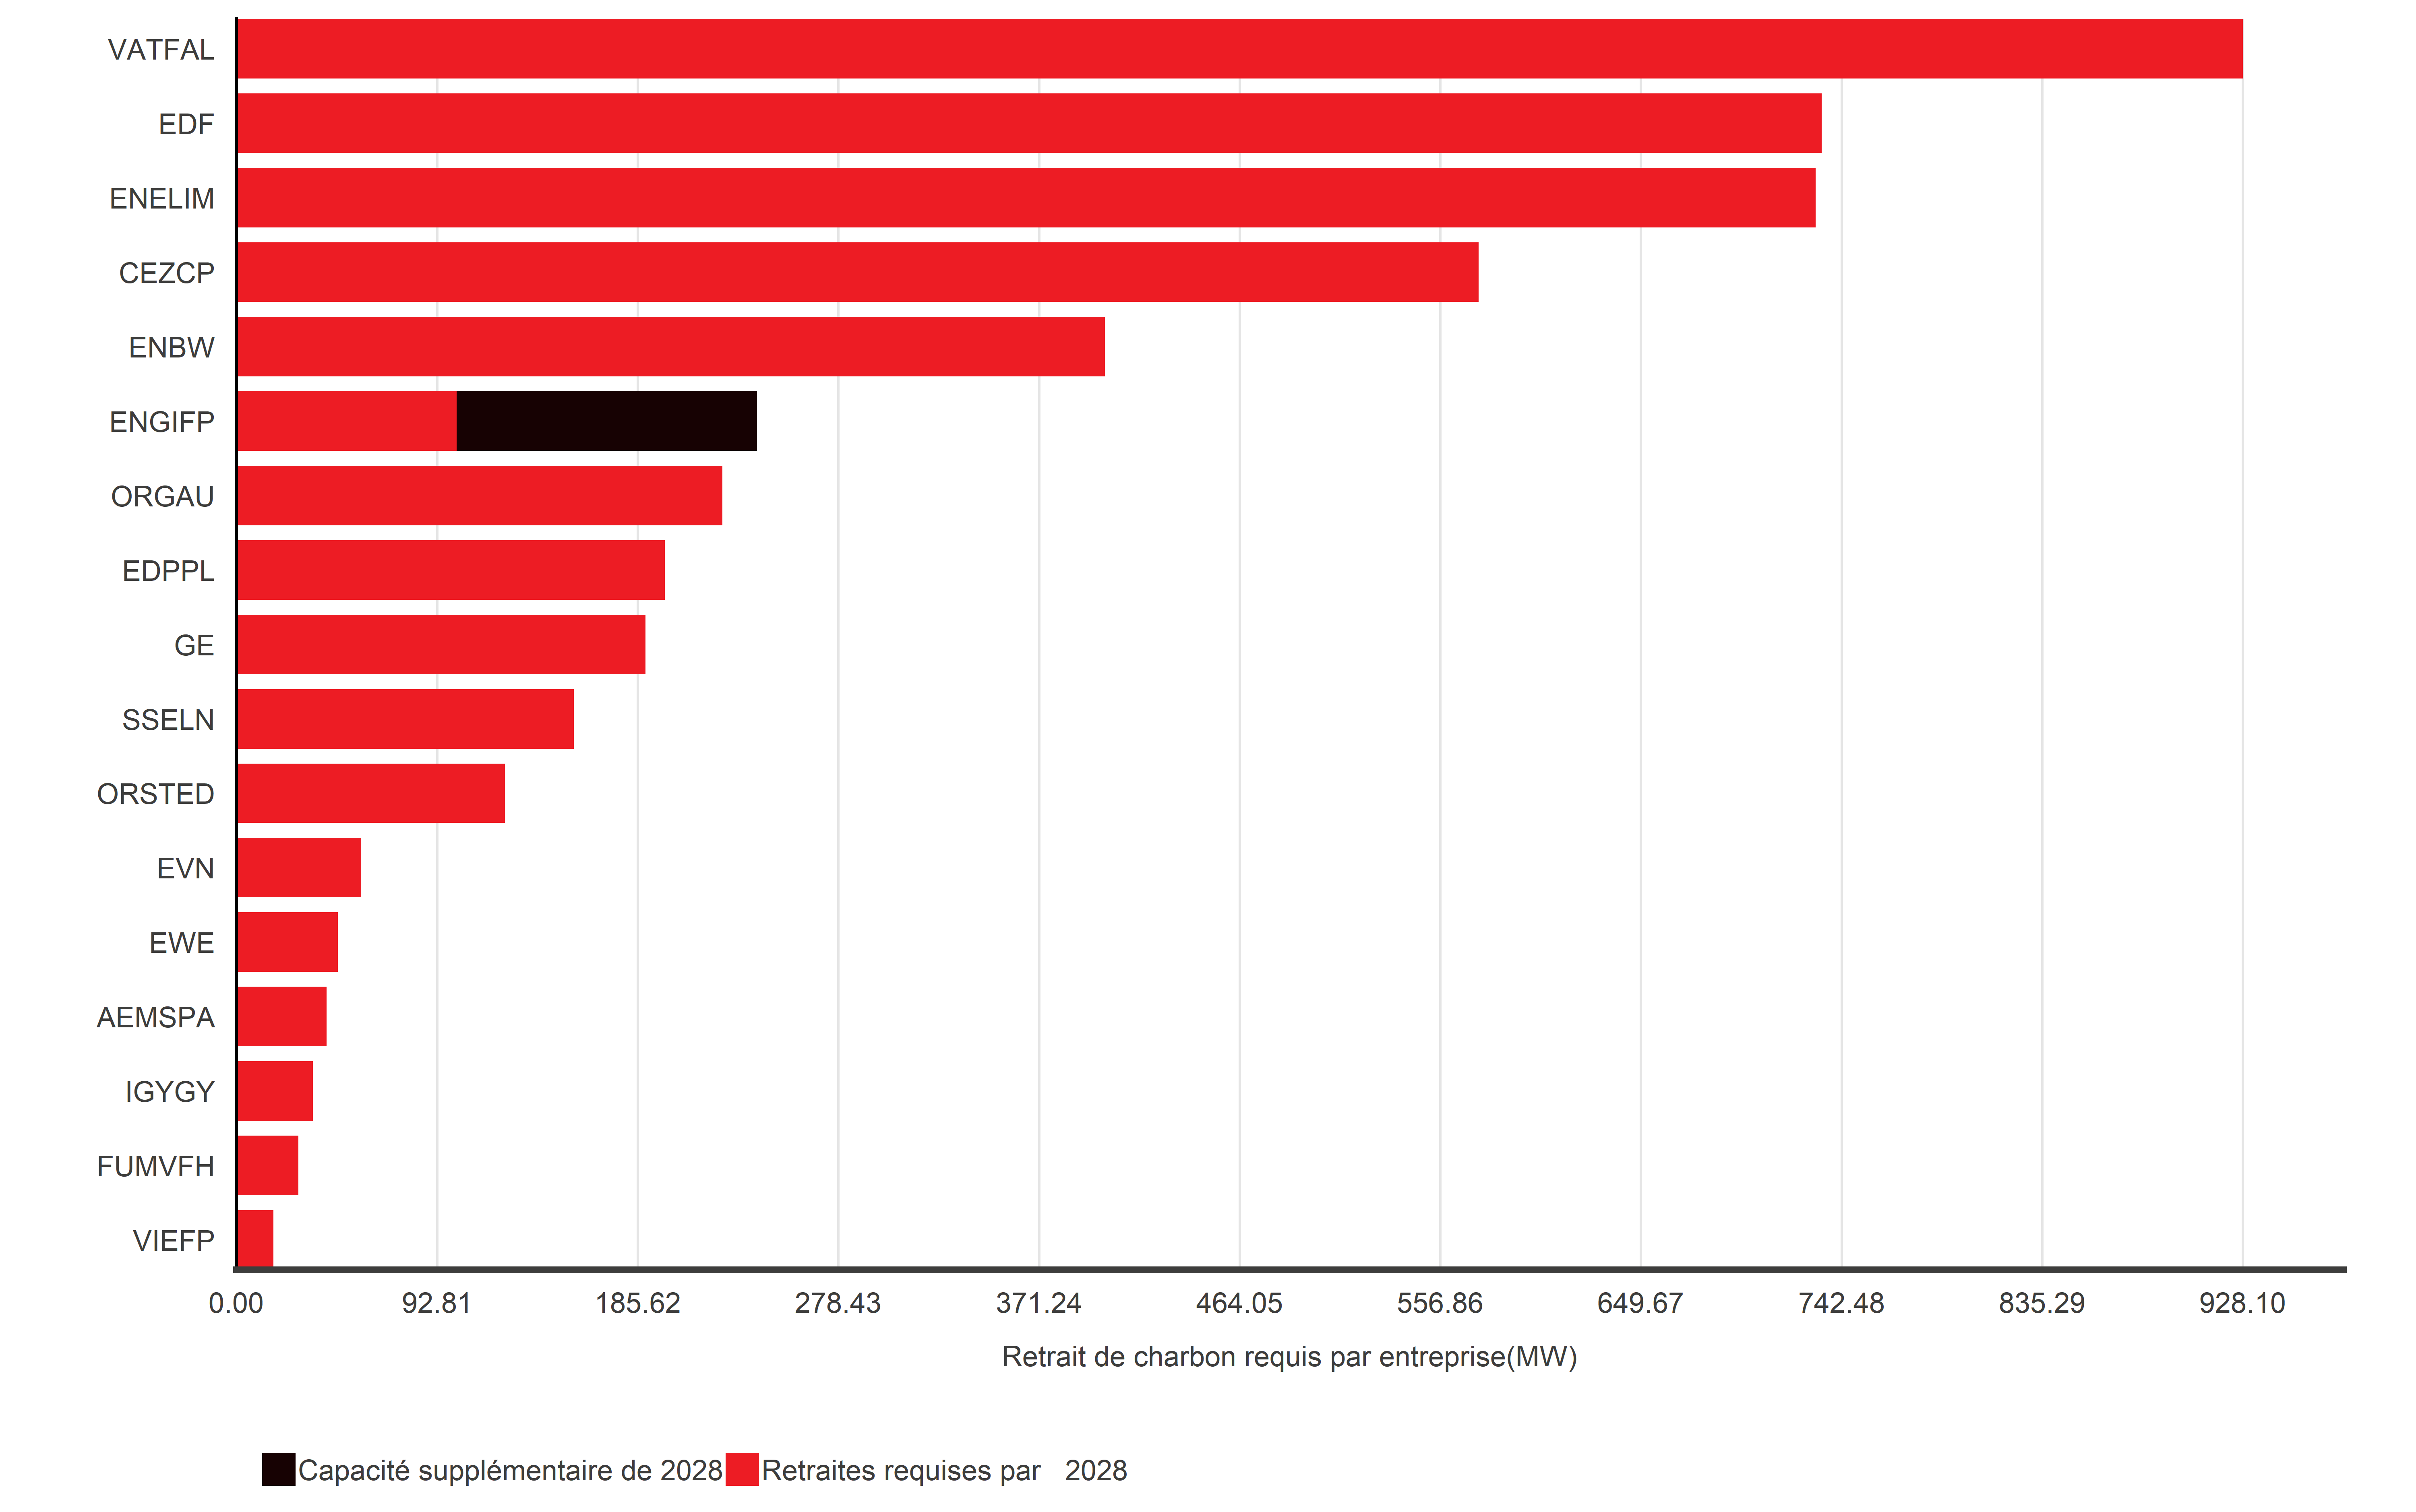
\includegraphics[trim = {0 0cm 0 0},width=0.85\linewidth]{ReportOutputs/Fig62}
	\end{center}
	%CBSpecificE
	
	%EQSpecificS	
	\textbf{Mises hors service et ajouts de capacités de production de charbon des entreprises dans le portefeuille actions}
	\vspace{-.0cm}
	
	\begin{center}
		\includegraphics[trim = {0 0cm 0 0},width=0.85\linewidth]{ReportOutputs/Fig63}
	\end{center}
	%EQSpecificE

	\PageFooterFifth
	\newpage 
	%CoalCapChartE
	%RenewableCapChartS
		\section*{} % COAL RETIREMENTS 
	\HeaderDouble{ENGAGEMENT ACTIONNARIAL}{ENERGIES RENOUVELABLES}
	
	\textbf{Les graphiques suivants montrent le développement de la capacité électrique issue des énergies renouvelables nécessaires pour que les entreprises des portefeuilles puissent atteindre la capacité requise d'ici  Startyear+5 dans le cadre du SDS.}
	
	La barre rouge indique la capacité supplémentaire nécessaire pour atteindre la capacité requise comme définie dans le SDS. La barre bleue montre la construction prévue au cours des cinq prochaines années. Le différentiel en capacité est indiqué en texte.

	
	%CBSpecificS
	\textbf{Ajout des capacités d’énergie renouvelable des entreprises dans le portefeuille d'obligations d’entreprises.}
	\vspace{-.0cm}
	
	\begin{center}
		\includegraphics[trim = {0 0cm 0 0},width=0.85\linewidth]{ReportOutputs/Fig64}
	\end{center}
	%CBSpecificE
	
	%EQSpecificS	
	\textbf{Ajout des capacités d’énergie renouvelable des entreprises dans le portefeuille actions.}
	\vspace{-.0cm}
	
	\begin{center}
		\includegraphics[trim = {0 0cm 0 0},width=0.85\linewidth]{ReportOutputs/Fig65}
	\end{center}
	%EQSpecificE
	
	\PageFooterFifth
	\newpage 
	%RenewableCapChartE
	%PowerSector_ALLE
	%CompanyChartsE
	\section*{} % 6th BACKGROUND
	\SectionHeading{SECTION 6:}{INFORMATIONS COMPLEMENTAIRES AU MODELE}
	\newpage
	\section*{} % CONTEXT p7
	\HeaderSingle{CONTEXTE}
	
	\begin{multicols}{2}
		{\small\textbf{Background.} En juin 2017, le Groupe de travail du Conseil de stabilité financière du G20 sur l'information financière relative au climat (TCFD) a recommandé que les institutions du G20 effectuent une analyse de scénarios sur leurs portefeuilles pour évaluer les risques liés au changement climatique. Le TCFD a regroupé les risques liés au climat en deux catégories: les risques physiques et les risques de transition. Les risques de transition sont les risques générés par les changements politiques, technologiques, commerciaux et réglementaires susceptibles d'accompagner la transition vers une économie bas carbone. 
		
		%UNPRI_TextS
		\textbf{PRI. }Principles for Responsible Investments (PRI)  est le plus grand réseau d’investisseurs au monde dans le domaine de l’investissement responsable, avec presque 2 000 signataires. 
		
		PRI s’efforce de comprendre les liens entre l’investissement et les facteurs environnementaux, sociaux et de gouvernance (ESG) et d’aider son réseau international d'investisseurs signataires à intégrer ces facteurs dans leurs décisions d’investissement et de management. Le changement climatique est la priorité ESG la plus important pour les investisseurs. Le PRI travaille à aider les investisseurs à protéger leurs portefeuilles contre les risques et à les exposer aux opportunités offertes par la transition énergétique.
		%UNPRI_TextE
		
		\textbf{But de l'analyse.} L'objectif de ce rapport d'analyse de scénarios est d'évaluer l'exposition des investisseurs aux risques de transition, individuellement et collectivement, en fonction de leur exposition actuelle et future (estimée) aux activités à forte et à faible intensité de carbone. Ce rapport présente les résultats de l'analyse par classe d'actif
		
		\textbf{Approche.} Les éléments clés de l'analyse sont les suivants:
		
		\begin{itemize}
			\item{\textit{Tendances actuelles et estimées de la production et des investissements.} La production actuelle et estimée (pour les secteurs des combustibles fossiles et de l'automobile) et la capacité installée actuelle et additionnelle prévue (pour le secteur de l'électricité) pour les cinq prochaines années proviennent des bases de données de fournisseurs commerciaux. Ces fournisseurs de données recueillent des données prospectives sur la production et la capacité au niveau des actifs physiques (nombre de barils de pétrole par puits, de voitures par modèle et par usine, et de capacité par centrale électrique). 2Dii associe ces données à leurs propriétaires directs et à la société mère pour calculer la production actuelle globale d'une entreprise (profil) pour chaque technologie. Ces plans de production sont liés aux titres financiers (actions et obligations de sociétés) émis par l'entreprise. Les données relevant du niveau des actifs, utilisées pour cette analyse ont été obtenues auprès de fournisseurs de données au cours du dernier semestre de 2018. Voir la section « Considérations et limites importantes » à la fin du rapport pour des notes sur l'interprétation des données sur la capacité du secteur de l'électricité.}
			
			\item{\textit{Allocation de la production d'actifs physiques aux actifs financiers.} En fonction de la part du total des capitaux propres ou de la dette détenue dans un portefeuille, le modèle attribue au portefeuille une partie des plans de production actuels de chaque société émettrice pour chaque technologie. En agrégeant l'ensemble des sociétés au niveau du portefeuille, le modèle définit le « profil de production » actuel du portefeuille pour une technologie.}
			
			\item{\textit{Des scénarios macro aux objectifs  micro.} Pour calculer les niveaux de production compatibles avec un scénario climatique tel que le SDD de l'AIE, le modèle utilise un principe de juste répartition (« fair share ») qui applique les changements selon le scénario pour une technologie et une région données de manière égale pour tous les détenteurs d'actifs physiques dans le secteur de cette technologie dans la région donnée. Cela crée un profil de production et de capacité prévisionnel compatible avec le scénario de chaque entreprise et de chaque technologie. Ces  profils  sont ensuite regroupés au niveau du portefeuille pour créer le « profil de production cible » du portefeuille dans le cadre du scénario. Ce profil est utilisé pour déterminer « l'exposition cible » de l'investisseur à une technologie dans le cadre du scénario. « L'exposition cible » ne requiert pas forcément de changement dans la composition du portefeuille: elle modélise les changements dans les plans de production et d'investissement qui sont requis pour l'ensemble des sociétés détenues dans le portefeuille afin de correspondre au déploiement technologique décrit dans le scénario.}
			
			\item{\textit{Analyse de l'intensité des émissions.} Pour les secteurs pour lesquels il n'y a pas de données disponibles sur les actifs ou les scénarios et pour lesquels il n'existe pas de technologie bas-carbone adoptée par le marché, une solution consiste à analyser les changements nécessaires dans l'intensité d'émissions. Pour ces secteurs, les efforts de décarbonisation porteront sur le dévelopement de méthodes de productions plus efficientes, ainsi que sur l'investissement dans la R\&D au cours des 5 à 10 prochaines années, afin d'amener à moyen terme des alternatives neutres en CO\textsubscript{2} à maturité commerciale. Par conséquent, les scénarios et les données sont relativement imprécis.}
\end{itemize}
		
		\textbf{Résultats de l'analyse de scénario.} 
		Le «profil cible» du portefeuille dans le cadre du scénario peut être comparé aux plans de production et d'investissements actuellement révélés du portefeuille pour chaque technologie afin de calculer l'exposition aux risques de transition, ainsi que la mesure dans laquelle le portefeuille devrait augmenter (ou diminuer!) l’alignement avec le ScenarioValue au cours des 5 prochaines années.}
		\newline	
		
	\end{multicols}
			
	\newpage
	
	
		
	\section*{} % BACKGROUND TO THE MODEL
	\HeaderSingle{INFORMATION COMPLEMENTAIRES AU MODELE}
	
	\begin{multicols}{2}
		
		
		{\small\textbf{Alignement sur la trajectoire de transition suivant un SDS.} Cette analyse évalue le niveau d'alignement avec une trajectoire de transition SDS, en utilisant deux références:
		
		\begin{itemize}
			\item{\textit{Le portefeuille dans le contexte d'une transition suivant le  ScenarioValue.} Il s'agit du profil de « production cible » du portefeuille sous le ScenarioValue: cela illustre les changements requis dans le profil de production des sociétés détenues dans le portefeuille, afin d'atteindre les objectifs de production et capacité du scénario, basé sur la méthodologie décrite ci-dessus. Étant donné que les titres détenus et leur poids dans le portefeuille sont identiques pour le portefeuille et ses versions alternatives, leur comparaison montre la mesure dans laquelle la production actuelle des sociétés détenues en portefeuille est ou non alignée avec chaque scénario. }
			
			\item{\textit{Le benchmark  ScenarioValue. }Il s'agit du profil de production cible pour le marché à l'échelle globale: dans le cadre du ScenarioValue, le rapport modélise le marché aligné. Le même principe que celui décrit ci-dessus s'applique à un « portefeuille de référence »: le marché des actions dans son ensemble, ou le marché des obligations d'entreprises dans son ensemble. Étant donné que les titres et leur poids dans le portefeuille de marché diffèrent par rapport à ceux du portefeuille, cette comparaison met en évidence un (non) alignement « idiosyncrasique ». En d'autres termes, il montre comment la composition actuelle du portefeuille affecte l'alignement avec les differents scénarios, lorsque le premier point souligne seulement les changements demandés aux entreprises.}
		\end{itemize}
		
		
		Le non alignement de la production d'un portefeuille et de l'exposition à chaque technologie par rapport à un scénario est un moyen de mieux comprendre l'exposition d'un investisseur aux risques de transition énergétique. Si des changements politiques, technologiques, réglementaires ou de marché  se produisent qui rendent l'économie réelle mondiale alignée avec le ScenarioValue, le mauvais alignement d'une technologie donnée modifierait probablement les rendements associés à ces actifs physiques sous-jacents. Toutefois, cette analyse n'évalue qu'une seule dimension des risques liés à la transition bas carbone: les actifs à risques dans l'économie réelle. Il ne tient pas compte de la résilience de l'entreprise face à ces changements et de sa capacité d'adaptation, ce qui nécessiterait une analyse plus approfondie. 
		
		
		\textbf{Scénarios.} Cette analyse de scénarios est basée sur des scénarios développés par l'AIE. Le scénario \textit{Beyond 2 degrees} (B2DS) se concentre sur la réalisation d'une croissance durable tout en limitant l'augmentation de la température à moins de 2°C. Le \textit{Sustainable Development Scenario }(SDS) a une approche plus holistique des problématiques durables et ne met pas seulement l'accent sur le changement climatique. En plus du SDS, l'AIE a également publié sur le site la définition pour le \textit{New Policies Scenario} (NPS) et le \textit{Current Policies Scenario} (CPS): ces derniers dessinent d'autres feuilles de route technologiques qui correspondent à une probabilité de 50\% de réchauffement maximum de 4°C et 6°C, respectivement. Le SDS, le NPS et le CPS fournissent tous des projections prospectives suffisamment détaillées au niveau régional pour permettre l'analyse de scénarios pour 11 technologies dans trois secteurs. 
		
	Le modèle utilise les indicateurs suivants des scénarios de l'Agence internationale de l'énergie auquel le portefeuille est comparé
		\begin{itemize}
			\item{Production d'électricité par combustible exprimée en MW  (e.g. énergies renouvelables, charbon, gaz, pétrole, hydroélectricité, nucléaire);}
			\item{Production de pétrole exprimée en barils de pétrole  / an;}
			\item{Production de gaz exprimée en m\textsuperscript{3} / an;}
			\item{Production de charbon exprimé en tonnes  / year;}
			%\item{Trajets des émissions de GES dans un échantillon de secteurs supplémentaires  (e.g. aviation, transport, ciment, acier).}
		\end{itemize}
		
		 
		\textbf{Données sur les actifs physiques.} Les données sur les actifs physiques proviennent des fournisseurs de données suivants: 
		\begin{itemize}
			\item{GlobalData (données sur les centrales électriques, y compris leur classification: actives, annoncées, financées, partiellement actives, disponibles, temporairement arrêtées, en construction, en cours de réhabilitation et de modernisation; données actuelles de prévisionnelles sur la production de pétrole et de gaz jusqu'en Startyear+5, données sur l'extraction de charbon); }
			\item{WardsAuto (véhicules légers de tourisme, cela inclut les prévisions de production du BAU Startyear-Startyear+5); }
			\item{Bloomberg (données fifnancières);}
			\item{S\&P Cross-Reference Services (base de données des fonds);}
			\item{Morningstar (base de données des fonds). }
			
		\end{itemize}
		
		\textbf{Paramètres du modèle.} L'analyse de scénario présentée ici reflète une sélection de différents paramètres. Pour plus de détails sur ces paramètres et sur leurs implications sur www.transitionmonitor.com/backgroundinformation.}
		
		
		
	\end{multicols}
	
	
	
	\newpage
	
	\section*{} % BACKGROUND TO THE MODEL
	\HeaderSingle{INFORMATION COMPLEMENTAIRES AU MODELE}
	
	\begin{multicols}{2}
		
		
		{\small \textbf{CONSIDERATION ET LIMITES IMPORTANTES DANS L'INTERPRETATION DES RESULTATS.}
		
	 		\begin{itemize}
			\item{\textit{Niveau d'exigence des scénarios.} L'utilisation d'un scénario donné (B2DS, SDS, NPS, CPS) ne doit pas suggéreer la prééminence d'un scénario parmi les autres. De même, le choix des scénarios de l'AIE ne doit pas être interprété comme une validation par 2Dii des hypothèses sous-jacentes. L'AIE a historiquement prescrit des quantités importantes d'énergie nucléaire et de capture et de stockage du carbone dans ses scénarios, une hypothèse qui fait l'objet de débats au sein de la communauté scientifique sur les sujets énergie/climat. En outre, la communauté internationale a relevé son objectif mondial de 2°C à bien moins de 2°C pour le faire atteindre 1,5°C. Il est important de souligner que chaque investisseur peut et pourrait vouloir adopter un point de vue individuel sur un scénario possible de décarbonisation qui peut ou non être lié aux scénarios modélisés par l'Agence internationale de l'énergie.}
			
			\item{\textit{Une photo de la situation actuelle plutôt que des estimations.} Les données de production prévisionnelles sont basées sur les plans « révélés » actuels des entreprises et sont sujettes à changement. Les estimations ne doivent donc pas être interprétées comme des prévisions, mais plutôt comme les plans actuels des entreprises tels qu'estimés à partir de diverses sources d'information par les experts en veille économique de chaque industrie spécifiquement. Étant donné l'horizon à cinq ans, il est probable que ces plans changent d'une façon ou d'une autre au fil du temps. De même, les investisseurs sont susceptibles de modifier la composition de leur portefeuille au fil du temps. L'échéance des obligations de sociétés est généralement de l'ordre de 3 à 7 ans. La durée moyenne de détention d'une action par un gestionnaire de fonds est de 20 mois en moyenne. Toutefois, cette analyse se veut une évaluation ponctuelle des expositions futures dans les conditions actuelles.}
			
			\item{\textit{Projections du secteur électrique.} Contrairement aux données sur la production des secteurs des combustibles fossiles et de l'automobile, les données sur la capacité du secteur de l'électricité ne comprennent pas d'information sur les mises hors service prévues. Cela doit donc être interprété comme une mesure de la capacité actuellement immobilisée et non comme une prévision de la capacité future. Les mises hors service ne sont pas inclues pour plusieurs raisons: Premièrement, la disponibilité des données varie énormément d'une administration et d'une région à l'autre, ainsi l'absence de données sur les mise hors service a été jugée plus représentative de la capacité du secteur que l'inclusion de données partielles.
				Deuxièmement, contrairement au secteur des combustibles fossiles où les puits de pétrole, le gisement de gaz et les mines de charbon cessent leur production lorsque leurs ressources sont épuisées, il est possible que les centrales électriques soient déclarées hors service ou même mises hors service pour ensuite reprendre leur production. Étant donné le niveau plus élevé d'incertitude entourant ce statut, ces informations ne sont pas incluses dans les projections du secteur de l'électricité utilisées dans l' analyse, et les projections de la capacité devraient donc être interprétées comme le « verrouillage » maximal potentiel de l'infrastructure actuelle. Dans le cas des technologies qui devraient diminuer dans le cadre du ScenarioValue, l'écart entre les projections de capacité actuelles et la capacité alignée au ScenarioValue devrait être considéré comme une estimation de la capacité qui devrait être retirée pour être en conformité avec le ScenarioValue.}
			
			\item{\textit{Intégration des stratégies ISR.} Le modèle s'appuie sur un « portefeuille de marché » diversifié, axé sur les technologies clefs figurant dans les feuilles de route de l'AIE. Par extension, les portefeuilles thématiques investis dans des technologies de pointe et/ou les portefeuilles ISR comportant un éventail de considérations environnementales, sociales et gouvernementales peuvent ne pas tenir compte de ces éléments.}
			
			
		\end{itemize}
	}
	\end{multicols}
	\newpage		
	
	\section*{} % CONTEXT p8
	\HeaderSingle{LES RISQUES DE TRANSITION POUR LES INVESTISSEURS}
	\begin{multicols}{2}
		{\small\textbf{Qu'est ce que les risques de transition ?} Les risques de transition se définissent au sens large en tant que risques économiques et financiers associés à la transition vers une économie à faible intensité carbone. La communauté internationale a défini un mandat pour limiter la contribution humaine au réchauffement climatique à bien en dessous de 2°C de réchauffement par rapport aux niveaux préindustriels. Selon les connaissances scientifique disponibles, l'atteinte de cet objectif nécessite la décarbonisation de l'économie au cours de ce siècle. Cette décarbonisation est vouée à avoir des répercussions majeures sur les secteurs à forte intensité carbone, dont les plus importantes porteront sur les combustibles fossiles, l'électricité, et les transports, qui contribuent à la majorité des émissions mondiales de gaz à effet de serre. 
		 
		
		Au fur et à mesure que l'économie se décarbonise, les entreprises qui ne parviennent pas à anticiper correctement cette transition sont susceptibles d'être exposées à des risques économiques. Les entreprises bien préparées à cette transition seront, à l'inverse, prêtes à capitaliser sur cette opportunité économique. De même, les risques économiques peuvent se traduire par des risques financiers sur les marchés si ils ne sont pas correctement anticipés par les acteurs des marchés financiers. 
		 
		
		La transition vers une économie à faible intensité carbone aura avoir des effets significatifs à court et à moyen terme. D'ici à l'année 2040 - dans 22 ans seulement - la production mondiale de charbon devrait diminuer de 46 \%, avec une baisse encore plus rapide attendue dans les marchés développés. La capacité mondiale de production d'électricité au charbon devrait à son tour diminuer de 41 \%. La production de véhicules à gazoline et diesel (véhicules à moteur à combustion interne) devrait diminuer de 21 \%. Cette baisse dans les activités à forte intensité carbone s'accompagnera également d'une réduction proportionnelle des émissions, obtenue grâce au déploiement des nouvelles technologies. La capacité d'énergies renouvelables et la production de véhicules électriques doit presque quadrupler en volume d'ici 2040. 
		
		
		L'analyse de scénarios peut aider les institutions financières à évaluer et, en fin de compte, à gérer les risques et les possibilités associés à la transition. En connaissance de cause, l'analyse de scénarios a été appliquée par des centaines d'institutions financières et d'instances de contrôle financier à ce jour. Cela constitue la base des recommandations TCFD. Le TCFD note que « les évaluations prospectives des activités concernant les questions liées au climat sont importantes pour les investisseurs et les autres parties prenantes pour comprendre le degré de vulnérabilité des organisations individuelles vis-à-vis des risques physiques et de transition et concernant la façon dont ces risques se manifestent ou sont pris en compte. Par conséquent, la Task Force est convaincu que les organisations devraient utiliser l'analyse de scénarios pour évaluer les éventuelles implications commerciales, stratégiques et financières des risques liés au climat et des opportunités, et rendre celles-ci publiques. » (TCFD Final Report, p. 33).
		
		Pour clarifier sa recommandation sur l'analyse des scénarios, la Task Force explique, « Un type clé de scénario de risque de transition est le scénario appelé 2°C,
		qui établit un cheminement et une trajectoire d'émissions cohérents avec le maintien de l'augmentation de la température moyenne mondiale à 2°C au-dessus des niveaux préindustriels. » (Rapport final du TCFD, p. 35).
		
		
	Si l'on part de ce principe, le rapport met en évidence les points suivants: pour le portefeuille, l'exposition actuelle aux risques de transition dans le secteur fossile, carburant, de l'énergie et de l'automobile, l'évolution du portefeuille par rapport au fil de temps dans ces secteurs par rapport au scénario à 2°C, et l'encours futur estimé sur la base de ces tendances. Bien que ces secteurs ne représentent pas toutes les activités et tous les secteurs à forte intensité carbone, ils représentent à la fois la plus grande part d'un portefeuille typique et la contribution la plus importante au changement climatique à l'heure actuelle, en plus de bénéficier de scénarios bien élaborés. 
		
Le rapport ne fournit pas d'estimations spécifiques quant à la perte potentielle de valeur qui pourrait être réalisée dans le portefeuille si ces risques se matérialisaient, ce qui est évidemment associé à une grande incertitude et une myriade d'hypothèses de modélisation. Pour chaque titre financier, la perte potentielle peut varier de 0 à 100 \% et peut même être associée à des rendements positifs, en fonction de la capacité d'adaptation de l'entreprise, l'anticipation de la tendance par les marchés financiers et la nature d'une réévaluation potentielle. C'est à la bonne anticipation de ces risques que ce rapport s'efforce de contribuer.}




		
	\vspace{-0.4cm}	
		
	\end{multicols}
	{\small
	\textbf{Changement de volume d'ici 2023 et 2040 selon le scénario 450S.}
	\begin{center}
		{\setlength{\tabcolsep}{10pt} % Default value: 6pt
			\renewcommand{\arraystretch}{1} % Default value: 1
			\begin{tabular}{ p{.24\linewidth}| P{.24\linewidth}| P{.24\linewidth}}
				\hline
				\textbf{technologie} & \textbf{Changement Total de Volume par 2023} & \textbf{Changement Total de Volume par 2040} \\ 
				\hline
				Energie renouvelable & 69\% \nearr{ColGreen} & 354\% \uparr{ColGreen}\\
				Energie hydroélectrique & 13\% \nearr{ColGreen} & 59\% \nearr{ColGreen}\\
				Energie Nucléaire & 17\% \nearr{ColGreen} & 89\% \nearr{ColGreen}\\
				Energie de Gaz & 8\% \nearr{ColGreen} & 31\% \nearr{ColGreen}\\
				Energie de Charbon & -3\% \searr{ColRed} & -41\% \searr{ColRed}\\				
				\hline
				Production pÉtroliere & -2\% \searr{ColRed} & -23\% \searr{ColRed}\\
				Production de Gaz & 5\% \nearr{ColGreen} & 8\% \nearr{ColGreen}\\
				Production de charbon & -11\% \searr{ColRed}& -46\% \searr{ColRed}\\ 
				\hline
				Production voitures à combustion  & -9\% \searr{ColRed} & -21\% \searr{ColRed}\\
				Production Voitures Hybrides & 97\% \uparr{ColGreen} & 440\% \uparr{ColGreen}\\
				Production Voitures Electriques & 105\% \uparr{ColGreen} & 352\% \uparr{ColGreen}\\
				\hline
			\end{tabular}
		}
	\end{center}
}
	{\small\textit{Source: IEA World Energy Outlook 2016}}
	
	
	\newpage
	\section*{} % UNDERSTANDING THE POWER SECTOR
	\HeaderSingle{COMPRENDRE LE SECTEUR DE L'ELECTRICITE}	
	
	
	\begin{multicols}{2}
		
		{\small L'analyse du portefeuille d'électricité est fondée sur l'analyse prospective des projections de capacité ajoutée, combustible par combustible, au cours des cinq prochaines années, selon le fournisseur d'informations commerciales GlobalData. L'horizon temporel de cinq ans correspond à la l'horizon de planification des investissements des ajouts de capacité de production d'électricité. Il est admis que les horizons de planification pour des investissements spécifiques peuvent être soit plus longs, soit plus courts. Une analyse à plus long terme ne permettrait pas d'identifier les ajouts significatifs actuellement en cours de planification par les entreprises, d'où l'horizon de 5 ans. Les tableaux d'information de la compagnie ne tiennent pas compte des ajouts de capacité prévus par les entreprises extérieures au secteur de l'électricité (par exemple les entreprises des technologies de l'information qui construisent des parcs éoliens pour alimenter leurs centres de données). L'évolution du portefeuille repose sur les ajouts de capacité prévus par les entreprises, pondérés selon leur poids relatif dans le portefeuille.
		 
		 
		Il est important de noter que les données sur les déclassements annoncés ou officiellement prévus des actifs de production d’énergie ne sont pas pris en compte dans l'analyse présentée ici. C'est intentionnel, étant donné le manque de données connexes et le désir de montrer les déclassements requis. En ce qui concerne les technologies qui devraient diminuer dans le ScenarioValue, l'écart entre les projections de capacité actuelles et la capacité cohérente avec le ScenarioValue doit être considérée comme une estimation de la capacité qui devrait être retirée pour être alignée avec le ScenarioValue.
		
		
	Tel qu'indiqué ci-dessus, les scénarios sont fondés sur les tendances mondiales, misent à l'échelle du portefeuille selon l'approche de la ‘fair share’. 
	
		
		Pour le secteur électrique, cette approche ne rend pas compte de l’évolution des parts de marché  de toutes les classes d'actifs et de tous les acteurs, notamment concernant l'augmentation de la capacité d'énergie renouvelable des ménages (par exemple, l'énergie solaire sur les toits), qui devrait modifier le marché de l'électricité.
		
		Alors que cette tendance implique qu'en pratique les entreprises sont susceptibles de perdre des parts de marché, elle n'est intentionnellement pas prise en compte dans l'analyse, afin de documenter la perte potentielle de parts de marché dans un ScenarioValue - et par extension le risque potentiel cumulatif de transition. Dans un scénario 2°C, le secteur de l'électricité se décarbonisera, et sa part dans la demande totale en énergie augmentera. L'Agence internationale de l'énergie (AIE) affirme que, dans un scénario à 2°C:
		
		
		« L'approvisionnement en électricité va se diversifier à l'échelle mondiale et se décarboniser avec une production bas-carbone dépassant celle du charbon avant 2020. La part de la production d'électricité au charbon devrait diminuer de 40\% aujourd'hui à 28\% en 2040. D'ici là, l'énergie éolienne, solaire et bioénergétique, et les énergies renouvelables combinées augmenteront leur part de marché de 6\% à 20\% » (IEA World Energy Outlook 2016, p. 241).
		
		
		La répartition parmi les technologies varie grandement selon le scénario. La production d'électricité au charbon augmentera selon les tendances actuelles mais diminue dans un scénario 2°C.
		
		
		Les investisseurs en actions et en obligations d’entreprise sont exposés à ces tendances par l'intermédiaire des instruments financiers émis par les entreprises d'électricité. On estime que 28\% des actifs de production d'électricité sont détenus par des sociétés publiques et 19\% des actifs sont détenus par des entités étatiques cotées en bourse, par exemple des émetteurs d'obligations municipales (voir la figure ci-dessous).}
		
	\end{multicols}
	
	\begin{multicols}{2}
		
		\vspace{-.2cm}
		{\small\textbf{Mix électriques: Business as Usual et 2DS}}
		
		
		
		
		\adjincludegraphics[width = .95\linewidth,trim={0cm 0cm 0cm .5cm},clip]{ReportGraphics/PowerLine.png}
		
		\textit{\small Source: IEA World Energy Outlook 2016
		}
	\par
		\vspace{0.5cm}
		
		{\small\textbf{Propriété des actifs de production d'électricité}}
		\newline
		
		\adjincludegraphics[width = .8\linewidth,trim={0cm 0cm 0cm 0.5cm},clip]{ReportGraphics/PowerPie.png}
		
		\textit{\small Source: IEA analysis and 2Dii, based on Platts, Bloomberg Professional service, Bloomberg New Energy Finance and national sources}
		
	\end{multicols}

%		
%	\newpage
%	\section*{} % EMISSIONS INTENSITY ANALYSIS
%	\HeaderSingle{ANALYSE DE L'INTENSITÉ DES ÉMISSIONS }
%	
%		\begin{multicols}{2}
%			
%			
%			\textbf{LA MÉTHODOLOGIE}
%			
%			Concernant l'analyse de l'intensité des émissions, une intensité d'émission est calculée pour chaque usine. Celles-ci sont ensuite agrégées au portefeuille en pondérant par le poids de l’entreprise au sein du portefeuille. Les données du scénario sont ensuite appliquées à ce point de départ et la trajectoire de réduction des émissions est calculée pour les cinq prochaines années. 
%			
%			Ces résultats peuvent servir de base à une discussion avec les entreprises de l'acier, du ciment, et du transport maritime en ce qui concerne leur stratégies pour atteindre la trajectoire pour chaque secteur.
%			 
%			
%				
%			\textbf{LES SCÉNARIOS} 
%			
%			La trajectoire de réduction de l'intensité des émissions repose sur les scénarios présentées dans l'ETP (Energy Technology Perspectives) 2017. La production et les émissions attendues pour les secteurs de l'acier et du ciment sont évaluées au niveau régional. Les trajectoires présentées dans ces secteur suivent le scénario 2°C. Le secteur du transport maritime ne dispose pas de suffisamment de données scénaristiques, et par conséquent le portefeuille est comparé au marché.
%			
%			
%			\textbf{L’ACIER} 
%			
%			Après les produits chimiques, la production d'acier est la deuxième plus grande consommatrice d'énergie parmi tous les secteurs industriels, et celle qui génère le plus de dioxyde de carbone. Le déploiement de fours à arc électrique est essentiel pour réduire les émissions (même si cette technologie reste émettrice de carbone). Le calcul d'une intensité moyenne pour chaque aciérie est basé sur la technologie utilisée, le combustible utilisé et les facteurs régionaux d'émissions du réseau électrique et de la consommation de combustibles, le cas échéant. Cette valeur est ensuite multipliée par la capacité de la centrale et un facteur de capacité choisi tant au niveau régional. Ces facteurs proviennent des bases de données de l'OCDE et de l'Association Mondiale de l’Acier.
%			  
%			
% 			\textbf{LE CIMENT}
% 			
%			La production de ciment est également d'un des secteurs les plus émetteurs. La production de béton représente environ 5\% des émissions anthropiques (Cement Sustainability Initiative). Cela concerne principalement la production de trois sources distinctes, le processus de calcination, la consommation d'énergie thermique et la consommation d'électricité. Le facteur d'émission est calculé en fonction des facteurs régionaux appliqués à chaque centrale. La majorité des données proviennent de Cement Sustainability Initiative.
%			 
%			
%			%\textbf{L’AVIATON}
%			
%			%Pour estimer les émissions actuelles de CO\textsubscript{2} de la flotte des avions, on a fait des hypothèses concernant les taux d'utilisation des aéronefs. Les émission sont été estimés pour chaque entreprise sur la base d'un passager-kilomètre; un équivalent pour les aéronefs utilisés uniquement pour le fret a été calculé. Il y a un niveau élevé d'incertitude dans cette méthodologie.
%			
%			
%			\textbf{LE SECTEUR MARITIME}
%			
%			Le meilleur indicateur actuel en matière d'évaluation de la durabilité du transport maritime est celui développé par Carbon War Room and Rightship. Chaque navire est classé de A à G, où A est le plus efficace des navires de chaque catégorie (p. ex. pétroliers, cargaisons, etc.). Le classement est calculé dynamiquement pour rendre compte des améliorations annuelles de l'efficience et des variations en moyenne, afin que les navires "A" soient toujours les plus performants (performance mesurée en termes d'intensité de  CO\textsubscript{2}. En l'absence de données scénaristiques, les résultats du secteur maritime du portefeuille sont comparés au marché.
%			
%			
%			
%			
%			
%		\end{multicols}	
%
%	

	
	
	
	\newpage
	%WWFSpecificIncludeE
	\section*{} % NOTES AND DISCLAIMER
	\HeaderSingle{REMARQUES}
	
	\begin{multicols}{2}
		{\small Les sources de données et de scénarios pour cette analyse sont fournies ci-dessous. 
		
		\textbf{RECHERCHE PUBLIÉE}
		
		La méthodologie à la base de ce scénario, les règles de calcul appliquées et des informations complémentaires sur les scénarios et les données figurent dans les documents de recherche suivants.
		
		PRINCIPES COMPTABLES: http://www.mdpi.com/2071-1050/ 10/2/328 
		
		Travail de Scénario : http://et-risk.eu/toolbox/ scenarios/ 
		
		Analyse des données au niveau des actifs: http://2degrees-investing.org/ IMG/pdf/assetdata\_v0.pdf
		
		\textbf{Sources pour l'analyse des données et des scénarios}
		
		Les données automobiles datent de juillet 2017 et sont fournies par WardsAuto / AutoForecastSolutions. Les données sur l'énergie sont de juillet 2017 et sont fournies par GlobalData. Les données sur la production de pétrole, de gaz et de charbon datent de fin 2018 et sont fournies par GlobalData. Lors de l'établissement de liens entre les données relatives aux actifs et les entreprises, les données utilisées sont celles fournies par les fournisseurs de données mentionnés ci-dessus et, dans la mesure du possible, enrichies avec des données Bloomberg. Toutes les données financières, ainsi que les numéros d'identification permettant de relier les données de l'entreprise aux instruments financiers, proviennent de Bloomberg. 
		
		Les voies de décarbonisation pour les autres secteurs proviennent de SBTI, qui fonde sa méthodologie sur les scénarios de l'AIE. Les scénarios pour le secteur de l'énergie et de l'électricité proviennent de l'ETP (AIE). Étant donné que le présent rapport ne contient pas d'informations sur les scénarios du secteur de l'automobile, les données connexes sont tirées de l'ETP. Les points de référence pour le secteur de l'électricité sont déterminés au niveau régional et appliqués en fonction des données d'exposition régionales, puis agrégés, pondérés en fonction de l'exposition régionale du portefeuille. Tous les autres résultats sont globaux.
		
		
		\textbf{Sources}
		
		Cement Sustainability Initiative (2018) https://www.wbcsdcement. org/index.php/key-issues/climate-protection
		
		Energy Technology Perspectives 2017 (2018) https://www.iea.org /etp/
		
		IPCC (2018) https://www.ipcc.ch/report/ar5/
		
		FSB (2018) https://www.fsb-tcfd.org/publications/final-recommendations-report/
		
		WoodMackenzie (2018) https://www.woodmac.com/news/ editorial/carbon-intensity-not-all-assets-are-created-equal/ 
		
		World Energy Outlook 2017 (2018) https://www.iea.org/weo2017/}
	
	\end{multicols}
	
	\newpage
	\newpage 

\end{document} 


